
\large

\chapter*{Particle Swarm Optimization}
\addcontentsline{toc}{chapter}{Particle Swarm Optimization}
Particle swarm optimization (PSO) has been successfully
applied to wide variety of problems in both of scientific and industrial
fields alongside with other swarm intelligence based techniques. It
undergoes beneath the umbrella of meta-heuristics where the global
solution is not guaranteed to be found for some class of problems , but
optimal or local solution can be easily found with few assumptions and
lower computation resources. Also, PSO is stochastic in its nature which
means the solution is not going to be the same for each time the
algorithm gets executed ; however, based on the bench-marking and some
handful testing, the final result fall contained within small region
inside the solution space.

PSO proved to be so efficient in terms of computational time and memory
compared to other methods. It also could be parallelized, but it is out
of this project's scope. The downside, however, is that PSO has some
hyper-parameters that have to be tuned to get reasonable solution within
small margin of error. This section will provide a mathematical and a
computational model of PSO.


\section{Introduction}

To understand the basic idea behind PSO, we have to know its origin.
This stochastic method was proposed by Dr. Eberhart and Dr. Kennedy in
1995 inspired by the social behavior of birds or groups of fish.

Imagine that there is a group of birds trying to find food which is
located only in one spot, none of the birds know exactly where the food
is ; however, they have an idea of how far away might the food be. So,
they have to cooperate intelligently to find the food spot.

In the same way, we have a bunch of particles (population), each one
represents a potential solution. None of the particle knows where is the
global minima of the objective function, but each particle has memory of
best visited location based on the value of the cost (objective)
function. Within each generation (new population), the best known
position to the population is updated for each iteration based on the
best fitness evaluated among this particular population.

\section{Mathematical Model of PSO}

Each particle has its own position vector
{\(\overset{\rightarrow}{x_{i}}(t)\)} and a velocity vector
{\(\overset{\rightarrow}{v_{i}}(t)\)} to update the position each
iteration along side with the particle's best known position
{\(\overset{\rightarrow}{P_{i}}(t)\)} and population's best know
position {\(\overset{\rightarrow}{g}(t)\)}. This can be modeled with
simple node has the aforementioned vectors and and another node
representing the new state of the particle after one iteration.

    \begin{figure}[htbp]
        \centering
        \scalebox{.8}{


\tikzset{every picture/.style={line width=0.75pt}} %set default line width to 0.75pt        

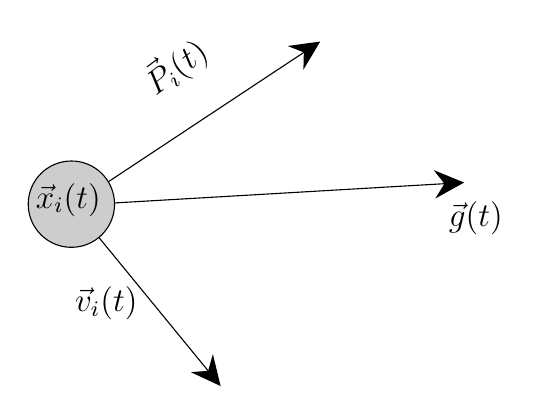
\begin{tikzpicture}[x=0.75pt,y=0.75pt,yscale=-1,xscale=1]
%uncomment if require: \path (0,300); %set diagram left start at 0, and has height of 300

%Straight Lines [id:da7251476173740483] 
\draw    (212,118) -- (397.61,107.17) ;
\draw [shift={(400.61,107)}, rotate = 176.66] [fill={rgb, 255:red, 0; green, 0; blue, 0 }  ][line width=0.08]  [draw opacity=0] (14.29,-6.86) -- (0,0) -- (14.29,6.86) -- (9.49,0) -- cycle    ;
%Straight Lines [id:da18169270686596173] 
\draw    (212,118) -- (328.81,40.71) ;
\draw [shift={(331.31,39.05)}, rotate = 146.51] [fill={rgb, 255:red, 0; green, 0; blue, 0 }  ][line width=0.08]  [draw opacity=0] (14.29,-6.86) -- (0,0) -- (14.29,6.86) -- (9.49,0) -- cycle    ;
%Straight Lines [id:da054979634098808905] 
\draw    (212,118) -- (281.41,202.73) ;
\draw [shift={(283.31,205.05)}, rotate = 230.68] [fill={rgb, 255:red, 0; green, 0; blue, 0 }  ][line width=0.08]  [draw opacity=0] (14.29,-6.86) -- (0,0) -- (14.29,6.86) -- (9.49,0) -- cycle    ;
%Shape: Circle [id:dp6795888605590055] 
\draw  [fill={rgb, 255:red, 205; green, 205; blue, 205 }  ,fill opacity=1 ] (190.61,117.4) .. controls (190.61,105.92) and (199.92,96.61) .. (211.4,96.61) .. controls (222.89,96.61) and (232.2,105.92) .. (232.2,117.4) .. controls (232.2,128.89) and (222.89,138.2) .. (211.4,138.2) .. controls (199.92,138.2) and (190.61,128.89) .. (190.61,117.4) -- cycle ;


% Text Node
\draw (392,115) node [anchor=north west][inner sep=0.75pt]  [font=\large]  {$\vec{g}( t)$};
% Text Node
\draw (193,106) node [anchor=north west][inner sep=0.75pt]  [font=\large]  {$\vec{x}_{i}( t)$};
% Text Node
\draw (241,52.96) node [anchor=north west][inner sep=0.75pt]  [font=\large,rotate=-323.22]  {$\vec{P_{i}}( t)$};
% Text Node
\draw (212,156) node [anchor=north west][inner sep=0.75pt]  [font=\large]  {$\vec{v}_{i}( t)$};


\end{tikzpicture}}
        \caption{Initial state of particle at point of time $t$ }
        \label{fig:label}
    \end{figure}
    


Each iteration, the position of the particle has to be updated, to do
so, the velocity vector must be updated first.\\
    \begin{figure}[htbp]
        \centering
        \scalebox{.7}{

\tikzset{every picture/.style={line width=0.75pt}} %set default line width to 0.75pt        

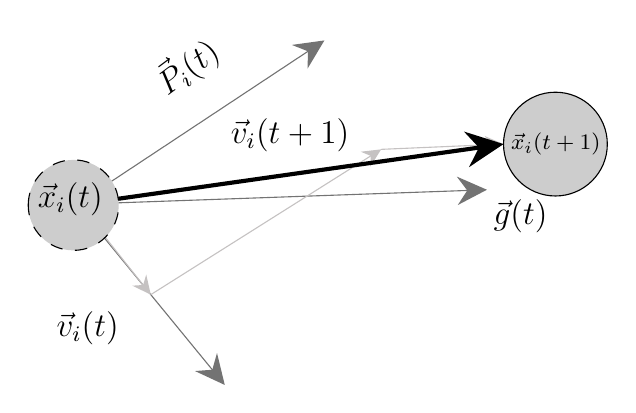
\begin{tikzpicture}[x=0.75pt,y=0.75pt,yscale=-1,xscale=1]
%uncomment if require: \path (0,300); %set diagram left start at 0, and has height of 300

%Straight Lines [id:da5958950638731724] 
\draw [color={rgb, 255:red, 115; green, 115; blue, 115 }  ,draw opacity=1 ]   (216,147) -- (410.61,140.11) ;
\draw [shift={(413.61,140)}, rotate = 177.97] [fill={rgb, 255:red, 115; green, 115; blue, 115 }  ,fill opacity=1 ][line width=0.08]  [draw opacity=0] (14.29,-6.86) -- (0,0) -- (14.29,6.86) -- (9.49,0) -- cycle    ;
%Straight Lines [id:da5519078451997654] 
\draw [color={rgb, 255:red, 115; green, 115; blue, 115 }  ,draw opacity=1 ]   (216,147) -- (332.81,69.71) ;
\draw [shift={(335.31,68.05)}, rotate = 146.51] [fill={rgb, 255:red, 115; green, 115; blue, 115 }  ,fill opacity=1 ][line width=0.08]  [draw opacity=0] (14.29,-6.86) -- (0,0) -- (14.29,6.86) -- (9.49,0) -- cycle    ;
%Straight Lines [id:da8436821411574322] 
\draw [color={rgb, 255:red, 115; green, 115; blue, 115 }  ,draw opacity=1 ]   (216,147) -- (285.41,231.73) ;
\draw [shift={(287.31,234.05)}, rotate = 230.68] [fill={rgb, 255:red, 115; green, 115; blue, 115 }  ,fill opacity=1 ][line width=0.08]  [draw opacity=0] (14.29,-6.86) -- (0,0) -- (14.29,6.86) -- (9.49,0) -- cycle    ;
%Straight Lines [id:da49229480545453086] 
\draw [color={rgb, 255:red, 197; green, 194; blue, 194 }  ,draw opacity=1 ]   (229,162) -- (249.79,188.18) ;
\draw [shift={(251.66,190.53)}, rotate = 231.54] [fill={rgb, 255:red, 197; green, 194; blue, 194 }  ,fill opacity=1 ][line width=0.08]  [draw opacity=0] (8.93,-4.29) -- (0,0) -- (8.93,4.29) -- (5.93,0) -- cycle    ;
%Straight Lines [id:da8102226735028486] 
\draw [color={rgb, 255:red, 197; green, 194; blue, 194 }  ,draw opacity=1 ]   (251.66,190.53) -- (360.12,122.13) ;
\draw [shift={(362.66,120.53)}, rotate = 147.76] [fill={rgb, 255:red, 197; green, 194; blue, 194 }  ,fill opacity=1 ][line width=0.08]  [draw opacity=0] (8.93,-4.29) -- (0,0) -- (8.93,4.29) -- (5.93,0) -- cycle    ;
%Straight Lines [id:da6537497146959208] 
\draw [color={rgb, 255:red, 197; green, 194; blue, 194 }  ,draw opacity=1 ]   (362.66,120.53) -- (418.61,118.13) ;
\draw [shift={(421.61,118)}, rotate = 177.55] [fill={rgb, 255:red, 197; green, 194; blue, 194 }  ,fill opacity=1 ][line width=0.08]  [draw opacity=0] (8.93,-4.29) -- (0,0) -- (8.93,4.29) -- (5.93,0) -- cycle    ;
%Shape: Circle [id:dp8574069381171916] 
\draw  [fill={rgb, 255:red, 205; green, 205; blue, 205 }  ,fill opacity=1 ] (421.61,118) .. controls (421.61,104.19) and (432.8,93) .. (446.61,93) .. controls (460.42,93) and (471.61,104.19) .. (471.61,118) .. controls (471.61,131.81) and (460.42,143) .. (446.61,143) .. controls (432.8,143) and (421.61,131.81) .. (421.61,118) -- cycle ;
%Straight Lines [id:da8931658978210233] 
\draw [line width=1.5]    (214.4,147.4) -- (417.65,118.56) ;
\draw [shift={(421.61,118)}, rotate = 171.92] [fill={rgb, 255:red, 0; green, 0; blue, 0 }  ][line width=0.08]  [draw opacity=0] (18.04,-8.67) -- (0,0) -- (18.04,8.67) -- (11.98,0) -- cycle    ;
%Shape: Circle [id:dp08907510762992255] 
\draw  [fill={rgb, 255:red, 205; green, 205; blue, 205 }  ,fill opacity=1 ][dash pattern={on 4.5pt off 4.5pt}] (192.61,147.4) .. controls (192.61,135.37) and (202.37,125.61) .. (214.4,125.61) .. controls (226.44,125.61) and (236.2,135.37) .. (236.2,147.4) .. controls (236.2,159.44) and (226.44,169.2) .. (214.4,169.2) .. controls (202.37,169.2) and (192.61,159.44) .. (192.61,147.4) -- cycle ;


% Text Node
\draw (289,104.4) node [anchor=north west][inner sep=0.75pt]  [font=\large]  {$\vec{v}_{i}( t+1)$};
% Text Node
\draw (424,111.4) node [anchor=north west][inner sep=0.75pt]  [font=\footnotesize]  {$\vec{x}_{i}( t+1)$};
% Text Node
\draw (415.61,143.4) node [anchor=north west][inner sep=0.75pt]  [font=\large]  {$\vec{g}( t)$};
% Text Node
\draw (196,135.4) node [anchor=north west][inner sep=0.75pt]  [font=\large]  {$\vec{x}_{i}( t)$};
% Text Node
\draw (248.64,82.49) node [anchor=north west][inner sep=0.75pt]  [font=\large,rotate=-323.22]  {$\vec{P_{i}}( t)$};
% Text Node
\draw (205,197.4) node [anchor=north west][inner sep=0.75pt]  [font=\large]  {$\vec{v}_{i}( t)$};


\end{tikzpicture}
}
        \caption{Initial state of particle at point of time $t$ }
        \label{fig:label}
    \end{figure}
    
As the figure shows, the velocity of each particle with a population can
be updated as follows:

\[\overset{\rightarrow}{v_{i}}(t + 1) = w.\overset{\rightarrow}{v_{i}}(t) + r_{1}.c_{1}.\lbrack\overset{\rightarrow}{P_{i}}(t) - \overset{\rightarrow}{x_{i}}(t)\rbrack + r_{2}.c_{2}.\lbrack\overset{\rightarrow}{g}(t) - \overset{\rightarrow}{x_{i}}(t)\rbrack\]

Where:

\begin{itemize}
\item
  {\(w\)} is the inertia weight (a scalar multiple of the velocity
  vector)
\item
  {\(r_{1}\)} and {\(r_{2}\)} are uniformly random numbers between 0 and
  1 {\(\rightarrow U\lbrack 0,1\rbrack\)}
\item
  {\(c_{1}\)} is cognitive weight (how the particle tends to be
  positioned towards the its best location)
\item
  {\(c_{2}\)} is social weight (how the particle tends to be positioned
  towards the global best location)
\end{itemize}

As we have a finite search space, the velocity vector has to fall within
a range:\\
{\[{\overset{\rightarrow}{v}}_{i}(t + 1) \in \lbrack{\overset{\rightarrow}{v}}_{min}\;,\;{\overset{\rightarrow}{v}}_{max}\rbrack\]}If
the condition does not prevail, the velocity is set to the extreme value
it has surpassed weather minimum or maximum.\\
After updating the velocity, the position vector can be update as
follows :\\
{\[{\overset{\rightarrow}{x}}_{i}(t + 1) = {\overset{\rightarrow}{x}}_{i}(t) + {\overset{\rightarrow}{v}}_{i}(t + 1)\]}Following
the last step, the best known position for the {\(i^{th}\)} particle can
be improved if the the following condition holds :\\
{\[f({\overset{\rightarrow}{x}}_{i}(t + 1)) < f({\overset{\rightarrow}{P}}_{i}(t))\ \;\Longrightarrow\;\ {\overset{\rightarrow}{P}}_{i}(t + 1) = {\overset{\rightarrow}{x}}_{i}(t + 1)\]}The
same way applies for the global best known position:\\
{\[f({\overset{\rightarrow}{P}}_{i}(t + 1)) < f(\overset{\rightarrow}{g}(t))\ \;\Longrightarrow\;\ \overset{\rightarrow}{g}(t + 1) = {\overset{\rightarrow}{P}}_{i}(t + 1)\]}Surely,
this is a simplified yet descriptive explanation of PSO; however, some
additional features can be added that can assist in fast convergence to
solution like simulating the death of a particle , which can be
described by :\\
{\[{\overset{\rightarrow}{x}}_{i}(t + 1) \notin \lbrack x_{max}\ ,\ x_{min}\rbrack\ \;\Longrightarrow\;\ {\overset{\rightarrow}{x}}_{i}(t + 1) = rand(\lbrack x_{max}\ ,\ x_{min}\rbrack)\]}Fairly
simple but still powerful to consider.

\section{PSO PseudoCode}

The pseudo-code of this algorithm is quite easy, we just have to compile
the equations stated above, all together yield :
\begin{algorithmic}
\State \textbf{Randomly} initialize Swarm population of $N$ particles $\vec{x}_i , 1 \le i \le N$
\State \textbf{Select} hyperparameter values $w$, $c_1$ and $c_2$
\For{$k \gets 1$ to $generations$}
    \For{$ i \gets 1$ to $N$}
        \State \textbf{a. Compute} new velocity of $i^{th}$ particle
            \State $\vec{v_i}(t+1) = w.\vec{v_i}(t)+
                    r_1.c_1.[\vec{P_i}(t)-\vec{x_i}(t)]+
                    r_2.c_2.[\vec{g}(t)-\vec{x_i}(t)]$
        \State \textbf{b. Check} new velocity bound 
            \If{$\vec{v}_i(t+1) < \vec{v}_{min}$}
                \State $\vec{v}_i(t+1) = \vec{v}_{min}$
            \ElsIf{$\vec{v}_i(t+1) > \vec{v}_{max}$}
                \State $\vec{v}_i(t+1) = \vec{v}_{max}$
            \EndIf
        \State \textbf{c. Update} the position of $i^{th}$ particle
        \State $\vec{x}_i(t+1)=\vec{x}_i(t) + \vec{v}_i(t+1)$
        \State \textbf{d. Update} new best of this particle and new best of Swarm
        \If{$f(\vec{x}_i(t+1)) < f(\vec{P}_i(t))$}
            \State $\vec{P}_i(t+1) = \vec{x}_i(t+1)$
        \EndIf
        \If{$f(\vec{P}_i(t+1)) < f(\vec{g}(t))$}
            \State $\vec{g}(t+1) = \vec{P}_i(t+1)$
        \EndIf
    \EndFor
\EndFor

\end{algorithmic}

\section{PSO Implementation}
PSO can be easily implemented in python  relying on OOP paradigm. It is very suitable for the purpose and and the algorithm can be further extended to adopt more techniques. I have implemented a particle class which contains the particle’s position, velocity, fitness, best position , and best fitness. That is besides a solver class to properly transfer the data between different  routines and export the necessary data for visualization. The following two figures are snapshots from the animation. In the first sub figure, the particle positions had been assigned randomly; after some iterations (generations), the particles tended to collaborate until they reached the minima of the objective function as clearly shown in the second sub-figure.
\begin{figure}[htp]
\begin{subfigure}{0.5\textwidth}
    \centering
   \scalebox{.6}{%% Creator: Matplotlib, PGF backend
%%
%% To include the figure in your LaTeX document, write
%%   \input{<filename>.pgf}
%%
%% Make sure the required packages are loaded in your preamble
%%   \usepackage{pgf}
%%
%% Also ensure that all the required font packages are loaded; for instance,
%% the lmodern package is sometimes necessary when using math font.
%%   \usepackage{lmodern}
%%
%% Figures using additional raster images can only be included by \input if
%% they are in the same directory as the main LaTeX file. For loading figures
%% from other directories you can use the `import` package
%%   \usepackage{import}
%%
%% and then include the figures with
%%   \import{<path to file>}{<filename>.pgf}
%%
%% Matplotlib used the following preamble
%%
\begingroup%
\makeatletter%
\begin{pgfpicture}%
\pgfpathrectangle{\pgfpointorigin}{\pgfqpoint{4.400164in}{4.041704in}}%
\pgfusepath{use as bounding box, clip}%
\begin{pgfscope}%
\pgfsetbuttcap%
\pgfsetmiterjoin%
\definecolor{currentfill}{rgb}{1.000000,1.000000,1.000000}%
\pgfsetfillcolor{currentfill}%
\pgfsetlinewidth{0.000000pt}%
\definecolor{currentstroke}{rgb}{1.000000,1.000000,1.000000}%
\pgfsetstrokecolor{currentstroke}%
\pgfsetdash{}{0pt}%
\pgfpathmoveto{\pgfqpoint{0.000000in}{0.000000in}}%
\pgfpathlineto{\pgfqpoint{4.400164in}{0.000000in}}%
\pgfpathlineto{\pgfqpoint{4.400164in}{4.041704in}}%
\pgfpathlineto{\pgfqpoint{0.000000in}{4.041704in}}%
\pgfpathlineto{\pgfqpoint{0.000000in}{0.000000in}}%
\pgfpathclose%
\pgfusepath{fill}%
\end{pgfscope}%
\begin{pgfscope}%
\pgfsetbuttcap%
\pgfsetmiterjoin%
\definecolor{currentfill}{rgb}{1.000000,1.000000,1.000000}%
\pgfsetfillcolor{currentfill}%
\pgfsetlinewidth{0.000000pt}%
\definecolor{currentstroke}{rgb}{0.000000,0.000000,0.000000}%
\pgfsetstrokecolor{currentstroke}%
\pgfsetstrokeopacity{0.000000}%
\pgfsetdash{}{0pt}%
\pgfpathmoveto{\pgfqpoint{0.100000in}{0.241704in}}%
\pgfpathlineto{\pgfqpoint{3.800000in}{0.241704in}}%
\pgfpathlineto{\pgfqpoint{3.800000in}{3.941704in}}%
\pgfpathlineto{\pgfqpoint{0.100000in}{3.941704in}}%
\pgfpathlineto{\pgfqpoint{0.100000in}{0.241704in}}%
\pgfpathclose%
\pgfusepath{fill}%
\end{pgfscope}%
\begin{pgfscope}%
\pgfsetbuttcap%
\pgfsetmiterjoin%
\pgfsetlinewidth{0.000000pt}%
\definecolor{currentstroke}{rgb}{1.000000,1.000000,1.000000}%
\pgfsetstrokecolor{currentstroke}%
\pgfsetstrokeopacity{0.000000}%
\pgfsetdash{}{0pt}%
\pgfpathmoveto{\pgfqpoint{0.552954in}{1.817046in}}%
\pgfpathlineto{\pgfqpoint{2.653838in}{2.245573in}}%
\pgfpathlineto{\pgfqpoint{2.685279in}{3.676404in}}%
\pgfpathlineto{\pgfqpoint{0.481032in}{3.274659in}}%
\pgfusepath{}%
\end{pgfscope}%
\begin{pgfscope}%
\pgfsetbuttcap%
\pgfsetmiterjoin%
\pgfsetlinewidth{0.000000pt}%
\definecolor{currentstroke}{rgb}{1.000000,1.000000,1.000000}%
\pgfsetstrokecolor{currentstroke}%
\pgfsetstrokeopacity{0.000000}%
\pgfsetdash{}{0pt}%
\pgfpathmoveto{\pgfqpoint{2.653838in}{2.245573in}}%
\pgfpathlineto{\pgfqpoint{3.532792in}{0.998439in}}%
\pgfpathlineto{\pgfqpoint{3.613728in}{2.503759in}}%
\pgfpathlineto{\pgfqpoint{2.685279in}{3.676404in}}%
\pgfusepath{}%
\end{pgfscope}%
\begin{pgfscope}%
\pgfsetbuttcap%
\pgfsetmiterjoin%
\pgfsetlinewidth{0.000000pt}%
\definecolor{currentstroke}{rgb}{1.000000,1.000000,1.000000}%
\pgfsetstrokecolor{currentstroke}%
\pgfsetstrokeopacity{0.000000}%
\pgfsetdash{}{0pt}%
\pgfpathmoveto{\pgfqpoint{0.552954in}{1.817046in}}%
\pgfpathlineto{\pgfqpoint{1.260160in}{0.484814in}}%
\pgfpathlineto{\pgfqpoint{3.532792in}{0.998439in}}%
\pgfpathlineto{\pgfqpoint{2.653838in}{2.245573in}}%
\pgfusepath{}%
\end{pgfscope}%
\begin{pgfscope}%
\pgfsetrectcap%
\pgfsetroundjoin%
\pgfsetlinewidth{0.803000pt}%
\definecolor{currentstroke}{rgb}{0.000000,0.000000,0.000000}%
\pgfsetstrokecolor{currentstroke}%
\pgfsetdash{}{0pt}%
\pgfpathmoveto{\pgfqpoint{0.552954in}{1.817046in}}%
\pgfpathlineto{\pgfqpoint{1.260160in}{0.484814in}}%
\pgfusepath{stroke}%
\end{pgfscope}%
\begin{pgfscope}%
\definecolor{textcolor}{rgb}{0.000000,0.000000,0.000000}%
\pgfsetstrokecolor{textcolor}%
\pgfsetfillcolor{textcolor}%
\pgftext[x=0.494748in,y=0.839342in,,]{\color{textcolor}\rmfamily\fontsize{20.000000}{24.000000}\selectfont \(\displaystyle x\)}%
\end{pgfscope}%
\begin{pgfscope}%
\pgfsetbuttcap%
\pgfsetroundjoin%
\pgfsetlinewidth{0.000000pt}%
\definecolor{currentstroke}{rgb}{0.000000,0.000000,0.000000}%
\pgfsetstrokecolor{currentstroke}%
\pgfsetdash{}{0pt}%
\pgfpathmoveto{\pgfqpoint{0.565877in}{1.792702in}}%
\pgfpathlineto{\pgfqpoint{2.669946in}{2.222717in}}%
\pgfpathlineto{\pgfqpoint{2.702219in}{3.655007in}}%
\pgfusepath{}%
\end{pgfscope}%
\begin{pgfscope}%
\pgfsetbuttcap%
\pgfsetroundjoin%
\pgfsetlinewidth{0.000000pt}%
\definecolor{currentstroke}{rgb}{0.000000,0.000000,0.000000}%
\pgfsetstrokecolor{currentstroke}%
\pgfsetdash{}{0pt}%
\pgfpathmoveto{\pgfqpoint{0.674599in}{1.587893in}}%
\pgfpathlineto{\pgfqpoint{2.805398in}{2.030526in}}%
\pgfpathlineto{\pgfqpoint{2.844780in}{3.474951in}}%
\pgfusepath{}%
\end{pgfscope}%
\begin{pgfscope}%
\pgfsetbuttcap%
\pgfsetroundjoin%
\pgfsetlinewidth{0.000000pt}%
\definecolor{currentstroke}{rgb}{0.000000,0.000000,0.000000}%
\pgfsetstrokecolor{currentstroke}%
\pgfsetdash{}{0pt}%
\pgfpathmoveto{\pgfqpoint{0.786586in}{1.376931in}}%
\pgfpathlineto{\pgfqpoint{2.944790in}{1.832746in}}%
\pgfpathlineto{\pgfqpoint{2.991692in}{3.289399in}}%
\pgfusepath{}%
\end{pgfscope}%
\begin{pgfscope}%
\pgfsetbuttcap%
\pgfsetroundjoin%
\pgfsetlinewidth{0.000000pt}%
\definecolor{currentstroke}{rgb}{0.000000,0.000000,0.000000}%
\pgfsetstrokecolor{currentstroke}%
\pgfsetdash{}{0pt}%
\pgfpathmoveto{\pgfqpoint{0.901990in}{1.159533in}}%
\pgfpathlineto{\pgfqpoint{3.088295in}{1.629129in}}%
\pgfpathlineto{\pgfqpoint{3.143159in}{3.098095in}}%
\pgfusepath{}%
\end{pgfscope}%
\begin{pgfscope}%
\pgfsetbuttcap%
\pgfsetroundjoin%
\pgfsetlinewidth{0.000000pt}%
\definecolor{currentstroke}{rgb}{0.000000,0.000000,0.000000}%
\pgfsetstrokecolor{currentstroke}%
\pgfsetdash{}{0pt}%
\pgfpathmoveto{\pgfqpoint{1.020968in}{0.935403in}}%
\pgfpathlineto{\pgfqpoint{3.236098in}{1.419413in}}%
\pgfpathlineto{\pgfqpoint{3.299395in}{2.900767in}}%
\pgfusepath{}%
\end{pgfscope}%
\begin{pgfscope}%
\pgfsetbuttcap%
\pgfsetroundjoin%
\pgfsetlinewidth{0.000000pt}%
\definecolor{currentstroke}{rgb}{0.000000,0.000000,0.000000}%
\pgfsetstrokecolor{currentstroke}%
\pgfsetdash{}{0pt}%
\pgfpathmoveto{\pgfqpoint{1.143690in}{0.704221in}}%
\pgfpathlineto{\pgfqpoint{3.388396in}{1.203319in}}%
\pgfpathlineto{\pgfqpoint{3.460629in}{2.697126in}}%
\pgfusepath{}%
\end{pgfscope}%
\begin{pgfscope}%
\pgfsetrectcap%
\pgfsetroundjoin%
\pgfsetlinewidth{1.304875pt}%
\definecolor{currentstroke}{rgb}{0.000000,0.000000,0.000000}%
\pgfsetstrokecolor{currentstroke}%
\pgfsetdash{}{0pt}%
\pgfpathmoveto{\pgfqpoint{0.583245in}{1.796252in}}%
\pgfpathlineto{\pgfqpoint{0.531114in}{1.785598in}}%
\pgfusepath{stroke}%
\end{pgfscope}%
\begin{pgfscope}%
\definecolor{textcolor}{rgb}{0.000000,0.000000,0.000000}%
\pgfsetstrokecolor{textcolor}%
\pgfsetfillcolor{textcolor}%
\pgftext[x=0.414440in,y=1.660690in,,top]{\color{textcolor}\rmfamily\fontsize{13.000000}{15.600000}\selectfont \(\displaystyle {0.0}\)}%
\end{pgfscope}%
\begin{pgfscope}%
\pgfsetrectcap%
\pgfsetroundjoin%
\pgfsetlinewidth{1.304875pt}%
\definecolor{currentstroke}{rgb}{0.000000,0.000000,0.000000}%
\pgfsetstrokecolor{currentstroke}%
\pgfsetdash{}{0pt}%
\pgfpathmoveto{\pgfqpoint{0.692195in}{1.591548in}}%
\pgfpathlineto{\pgfqpoint{0.639378in}{1.580577in}}%
\pgfusepath{stroke}%
\end{pgfscope}%
\begin{pgfscope}%
\definecolor{textcolor}{rgb}{0.000000,0.000000,0.000000}%
\pgfsetstrokecolor{textcolor}%
\pgfsetfillcolor{textcolor}%
\pgftext[x=0.520801in,y=1.454160in,,top]{\color{textcolor}\rmfamily\fontsize{13.000000}{15.600000}\selectfont \(\displaystyle {2.5}\)}%
\end{pgfscope}%
\begin{pgfscope}%
\pgfsetrectcap%
\pgfsetroundjoin%
\pgfsetlinewidth{1.304875pt}%
\definecolor{currentstroke}{rgb}{0.000000,0.000000,0.000000}%
\pgfsetstrokecolor{currentstroke}%
\pgfsetdash{}{0pt}%
\pgfpathmoveto{\pgfqpoint{0.804418in}{1.380696in}}%
\pgfpathlineto{\pgfqpoint{0.750896in}{1.369393in}}%
\pgfusepath{stroke}%
\end{pgfscope}%
\begin{pgfscope}%
\definecolor{textcolor}{rgb}{0.000000,0.000000,0.000000}%
\pgfsetstrokecolor{textcolor}%
\pgfsetfillcolor{textcolor}%
\pgftext[x=0.630353in,y=1.241431in,,top]{\color{textcolor}\rmfamily\fontsize{13.000000}{15.600000}\selectfont \(\displaystyle {5.0}\)}%
\end{pgfscope}%
\begin{pgfscope}%
\pgfsetrectcap%
\pgfsetroundjoin%
\pgfsetlinewidth{1.304875pt}%
\definecolor{currentstroke}{rgb}{0.000000,0.000000,0.000000}%
\pgfsetstrokecolor{currentstroke}%
\pgfsetdash{}{0pt}%
\pgfpathmoveto{\pgfqpoint{0.920062in}{1.163415in}}%
\pgfpathlineto{\pgfqpoint{0.865817in}{1.151764in}}%
\pgfusepath{stroke}%
\end{pgfscope}%
\begin{pgfscope}%
\definecolor{textcolor}{rgb}{0.000000,0.000000,0.000000}%
\pgfsetstrokecolor{textcolor}%
\pgfsetfillcolor{textcolor}%
\pgftext[x=0.743243in,y=1.022221in,,top]{\color{textcolor}\rmfamily\fontsize{13.000000}{15.600000}\selectfont \(\displaystyle {7.5}\)}%
\end{pgfscope}%
\begin{pgfscope}%
\pgfsetrectcap%
\pgfsetroundjoin%
\pgfsetlinewidth{1.304875pt}%
\definecolor{currentstroke}{rgb}{0.000000,0.000000,0.000000}%
\pgfsetstrokecolor{currentstroke}%
\pgfsetdash{}{0pt}%
\pgfpathmoveto{\pgfqpoint{1.039288in}{0.939406in}}%
\pgfpathlineto{\pgfqpoint{0.984299in}{0.927391in}}%
\pgfusepath{stroke}%
\end{pgfscope}%
\begin{pgfscope}%
\definecolor{textcolor}{rgb}{0.000000,0.000000,0.000000}%
\pgfsetstrokecolor{textcolor}%
\pgfsetfillcolor{textcolor}%
\pgftext[x=0.859626in,y=0.796230in,,top]{\color{textcolor}\rmfamily\fontsize{13.000000}{15.600000}\selectfont \(\displaystyle {10.0}\)}%
\end{pgfscope}%
\begin{pgfscope}%
\pgfsetrectcap%
\pgfsetroundjoin%
\pgfsetlinewidth{1.304875pt}%
\definecolor{currentstroke}{rgb}{0.000000,0.000000,0.000000}%
\pgfsetstrokecolor{currentstroke}%
\pgfsetdash{}{0pt}%
\pgfpathmoveto{\pgfqpoint{1.162263in}{0.708351in}}%
\pgfpathlineto{\pgfqpoint{1.106511in}{0.695954in}}%
\pgfusepath{stroke}%
\end{pgfscope}%
\begin{pgfscope}%
\definecolor{textcolor}{rgb}{0.000000,0.000000,0.000000}%
\pgfsetstrokecolor{textcolor}%
\pgfsetfillcolor{textcolor}%
\pgftext[x=0.979666in,y=0.563137in,,top]{\color{textcolor}\rmfamily\fontsize{13.000000}{15.600000}\selectfont \(\displaystyle {12.5}\)}%
\end{pgfscope}%
\begin{pgfscope}%
\pgfsetrectcap%
\pgfsetroundjoin%
\pgfsetlinewidth{0.803000pt}%
\definecolor{currentstroke}{rgb}{0.000000,0.000000,0.000000}%
\pgfsetstrokecolor{currentstroke}%
\pgfsetdash{}{0pt}%
\pgfpathmoveto{\pgfqpoint{3.532792in}{0.998439in}}%
\pgfpathlineto{\pgfqpoint{1.260160in}{0.484814in}}%
\pgfusepath{stroke}%
\end{pgfscope}%
\begin{pgfscope}%
\definecolor{textcolor}{rgb}{0.000000,0.000000,0.000000}%
\pgfsetstrokecolor{textcolor}%
\pgfsetfillcolor{textcolor}%
\pgftext[x=2.570508in,y=0.228034in,,]{\color{textcolor}\rmfamily\fontsize{20.000000}{24.000000}\selectfont \(\displaystyle y\)}%
\end{pgfscope}%
\begin{pgfscope}%
\pgfsetbuttcap%
\pgfsetroundjoin%
\pgfsetlinewidth{0.000000pt}%
\definecolor{currentstroke}{rgb}{0.000000,0.000000,0.000000}%
\pgfsetstrokecolor{currentstroke}%
\pgfsetdash{}{0pt}%
\pgfpathmoveto{\pgfqpoint{0.526568in}{3.282958in}}%
\pgfpathlineto{\pgfqpoint{0.596289in}{1.825886in}}%
\pgfpathlineto{\pgfqpoint{1.307175in}{0.495439in}}%
\pgfusepath{}%
\end{pgfscope}%
\begin{pgfscope}%
\pgfsetbuttcap%
\pgfsetroundjoin%
\pgfsetlinewidth{0.000000pt}%
\definecolor{currentstroke}{rgb}{0.000000,0.000000,0.000000}%
\pgfsetstrokecolor{currentstroke}%
\pgfsetdash{}{0pt}%
\pgfpathmoveto{\pgfqpoint{0.901080in}{3.351216in}}%
\pgfpathlineto{\pgfqpoint{0.952806in}{1.898606in}}%
\pgfpathlineto{\pgfqpoint{1.693747in}{0.582807in}}%
\pgfusepath{}%
\end{pgfscope}%
\begin{pgfscope}%
\pgfsetbuttcap%
\pgfsetroundjoin%
\pgfsetlinewidth{0.000000pt}%
\definecolor{currentstroke}{rgb}{0.000000,0.000000,0.000000}%
\pgfsetstrokecolor{currentstroke}%
\pgfsetdash{}{0pt}%
\pgfpathmoveto{\pgfqpoint{1.271476in}{3.418724in}}%
\pgfpathlineto{\pgfqpoint{1.305588in}{1.970564in}}%
\pgfpathlineto{\pgfqpoint{2.075883in}{0.669171in}}%
\pgfusepath{}%
\end{pgfscope}%
\begin{pgfscope}%
\pgfsetbuttcap%
\pgfsetroundjoin%
\pgfsetlinewidth{0.000000pt}%
\definecolor{currentstroke}{rgb}{0.000000,0.000000,0.000000}%
\pgfsetstrokecolor{currentstroke}%
\pgfsetdash{}{0pt}%
\pgfpathmoveto{\pgfqpoint{1.637821in}{3.485494in}}%
\pgfpathlineto{\pgfqpoint{1.654691in}{2.041773in}}%
\pgfpathlineto{\pgfqpoint{2.453657in}{0.754550in}}%
\pgfusepath{}%
\end{pgfscope}%
\begin{pgfscope}%
\pgfsetbuttcap%
\pgfsetroundjoin%
\pgfsetlinewidth{0.000000pt}%
\definecolor{currentstroke}{rgb}{0.000000,0.000000,0.000000}%
\pgfsetstrokecolor{currentstroke}%
\pgfsetdash{}{0pt}%
\pgfpathmoveto{\pgfqpoint{2.000183in}{3.551538in}}%
\pgfpathlineto{\pgfqpoint{2.000174in}{2.112242in}}%
\pgfpathlineto{\pgfqpoint{2.827145in}{0.838960in}}%
\pgfusepath{}%
\end{pgfscope}%
\begin{pgfscope}%
\pgfsetbuttcap%
\pgfsetroundjoin%
\pgfsetlinewidth{0.000000pt}%
\definecolor{currentstroke}{rgb}{0.000000,0.000000,0.000000}%
\pgfsetstrokecolor{currentstroke}%
\pgfsetdash{}{0pt}%
\pgfpathmoveto{\pgfqpoint{2.358625in}{3.616868in}}%
\pgfpathlineto{\pgfqpoint{2.342093in}{2.181985in}}%
\pgfpathlineto{\pgfqpoint{3.196418in}{0.922417in}}%
\pgfusepath{}%
\end{pgfscope}%
\begin{pgfscope}%
\pgfsetrectcap%
\pgfsetroundjoin%
\pgfsetlinewidth{1.304875pt}%
\definecolor{currentstroke}{rgb}{0.000000,0.000000,0.000000}%
\pgfsetstrokecolor{currentstroke}%
\pgfsetdash{}{0pt}%
\pgfpathmoveto{\pgfqpoint{1.300945in}{0.507100in}}%
\pgfpathlineto{\pgfqpoint{1.319665in}{0.472065in}}%
\pgfusepath{stroke}%
\end{pgfscope}%
\begin{pgfscope}%
\definecolor{textcolor}{rgb}{0.000000,0.000000,0.000000}%
\pgfsetstrokecolor{textcolor}%
\pgfsetfillcolor{textcolor}%
\pgftext[x=1.366127in,y=0.284925in,,top]{\color{textcolor}\rmfamily\fontsize{13.000000}{15.600000}\selectfont \(\displaystyle {0.0}\)}%
\end{pgfscope}%
\begin{pgfscope}%
\pgfsetrectcap%
\pgfsetroundjoin%
\pgfsetlinewidth{1.304875pt}%
\definecolor{currentstroke}{rgb}{0.000000,0.000000,0.000000}%
\pgfsetstrokecolor{currentstroke}%
\pgfsetdash{}{0pt}%
\pgfpathmoveto{\pgfqpoint{1.687257in}{0.594333in}}%
\pgfpathlineto{\pgfqpoint{1.706758in}{0.559701in}}%
\pgfusepath{stroke}%
\end{pgfscope}%
\begin{pgfscope}%
\definecolor{textcolor}{rgb}{0.000000,0.000000,0.000000}%
\pgfsetstrokecolor{textcolor}%
\pgfsetfillcolor{textcolor}%
\pgftext[x=1.753594in,y=0.373790in,,top]{\color{textcolor}\rmfamily\fontsize{13.000000}{15.600000}\selectfont \(\displaystyle {2.5}\)}%
\end{pgfscope}%
\begin{pgfscope}%
\pgfsetrectcap%
\pgfsetroundjoin%
\pgfsetlinewidth{1.304875pt}%
\definecolor{currentstroke}{rgb}{0.000000,0.000000,0.000000}%
\pgfsetstrokecolor{currentstroke}%
\pgfsetdash{}{0pt}%
\pgfpathmoveto{\pgfqpoint{2.069139in}{0.680565in}}%
\pgfpathlineto{\pgfqpoint{2.089402in}{0.646330in}}%
\pgfusepath{stroke}%
\end{pgfscope}%
\begin{pgfscope}%
\definecolor{textcolor}{rgb}{0.000000,0.000000,0.000000}%
\pgfsetstrokecolor{textcolor}%
\pgfsetfillcolor{textcolor}%
\pgftext[x=2.136600in,y=0.461632in,,top]{\color{textcolor}\rmfamily\fontsize{13.000000}{15.600000}\selectfont \(\displaystyle {5.0}\)}%
\end{pgfscope}%
\begin{pgfscope}%
\pgfsetrectcap%
\pgfsetroundjoin%
\pgfsetlinewidth{1.304875pt}%
\definecolor{currentstroke}{rgb}{0.000000,0.000000,0.000000}%
\pgfsetstrokecolor{currentstroke}%
\pgfsetdash{}{0pt}%
\pgfpathmoveto{\pgfqpoint{2.446665in}{0.765815in}}%
\pgfpathlineto{\pgfqpoint{2.467673in}{0.731969in}}%
\pgfusepath{stroke}%
\end{pgfscope}%
\begin{pgfscope}%
\definecolor{textcolor}{rgb}{0.000000,0.000000,0.000000}%
\pgfsetstrokecolor{textcolor}%
\pgfsetfillcolor{textcolor}%
\pgftext[x=2.515221in,y=0.548469in,,top]{\color{textcolor}\rmfamily\fontsize{13.000000}{15.600000}\selectfont \(\displaystyle {7.5}\)}%
\end{pgfscope}%
\begin{pgfscope}%
\pgfsetrectcap%
\pgfsetroundjoin%
\pgfsetlinewidth{1.304875pt}%
\definecolor{currentstroke}{rgb}{0.000000,0.000000,0.000000}%
\pgfsetstrokecolor{currentstroke}%
\pgfsetdash{}{0pt}%
\pgfpathmoveto{\pgfqpoint{2.819911in}{0.850097in}}%
\pgfpathlineto{\pgfqpoint{2.841644in}{0.816635in}}%
\pgfusepath{stroke}%
\end{pgfscope}%
\begin{pgfscope}%
\definecolor{textcolor}{rgb}{0.000000,0.000000,0.000000}%
\pgfsetstrokecolor{textcolor}%
\pgfsetfillcolor{textcolor}%
\pgftext[x=2.889533in,y=0.634317in,,top]{\color{textcolor}\rmfamily\fontsize{13.000000}{15.600000}\selectfont \(\displaystyle {10.0}\)}%
\end{pgfscope}%
\begin{pgfscope}%
\pgfsetrectcap%
\pgfsetroundjoin%
\pgfsetlinewidth{1.304875pt}%
\definecolor{currentstroke}{rgb}{0.000000,0.000000,0.000000}%
\pgfsetstrokecolor{currentstroke}%
\pgfsetdash{}{0pt}%
\pgfpathmoveto{\pgfqpoint{3.188949in}{0.933429in}}%
\pgfpathlineto{\pgfqpoint{3.211390in}{0.900344in}}%
\pgfusepath{stroke}%
\end{pgfscope}%
\begin{pgfscope}%
\definecolor{textcolor}{rgb}{0.000000,0.000000,0.000000}%
\pgfsetstrokecolor{textcolor}%
\pgfsetfillcolor{textcolor}%
\pgftext[x=3.259607in,y=0.719194in,,top]{\color{textcolor}\rmfamily\fontsize{13.000000}{15.600000}\selectfont \(\displaystyle {12.5}\)}%
\end{pgfscope}%
\begin{pgfscope}%
\pgfsetrectcap%
\pgfsetroundjoin%
\pgfsetlinewidth{0.803000pt}%
\definecolor{currentstroke}{rgb}{0.000000,0.000000,0.000000}%
\pgfsetstrokecolor{currentstroke}%
\pgfsetdash{}{0pt}%
\pgfpathmoveto{\pgfqpoint{3.532792in}{0.998439in}}%
\pgfpathlineto{\pgfqpoint{3.613728in}{2.503759in}}%
\pgfusepath{stroke}%
\end{pgfscope}%
\begin{pgfscope}%
\definecolor{textcolor}{rgb}{0.000000,0.000000,0.000000}%
\pgfsetstrokecolor{textcolor}%
\pgfsetfillcolor{textcolor}%
\pgftext[x=4.204293in, y=1.238368in, left, base,rotate=86.922333]{\color{textcolor}\rmfamily\fontsize{18.000000}{21.600000}\selectfont \(\displaystyle f(x,y)\)}%
\end{pgfscope}%
\begin{pgfscope}%
\pgfsetbuttcap%
\pgfsetroundjoin%
\pgfsetlinewidth{0.000000pt}%
\definecolor{currentstroke}{rgb}{0.000000,0.000000,0.000000}%
\pgfsetstrokecolor{currentstroke}%
\pgfsetdash{}{0pt}%
\pgfpathmoveto{\pgfqpoint{3.537656in}{1.088918in}}%
\pgfpathlineto{\pgfqpoint{2.655735in}{2.331938in}}%
\pgfpathlineto{\pgfqpoint{0.548619in}{1.904900in}}%
\pgfusepath{}%
\end{pgfscope}%
\begin{pgfscope}%
\pgfsetbuttcap%
\pgfsetroundjoin%
\pgfsetlinewidth{0.000000pt}%
\definecolor{currentstroke}{rgb}{0.000000,0.000000,0.000000}%
\pgfsetstrokecolor{currentstroke}%
\pgfsetdash{}{0pt}%
\pgfpathmoveto{\pgfqpoint{3.562675in}{1.554230in}}%
\pgfpathlineto{\pgfqpoint{2.665479in}{2.775358in}}%
\pgfpathlineto{\pgfqpoint{0.526350in}{2.356224in}}%
\pgfusepath{}%
\end{pgfscope}%
\begin{pgfscope}%
\pgfsetbuttcap%
\pgfsetroundjoin%
\pgfsetlinewidth{0.000000pt}%
\definecolor{currentstroke}{rgb}{0.000000,0.000000,0.000000}%
\pgfsetstrokecolor{currentstroke}%
\pgfsetdash{}{0pt}%
\pgfpathmoveto{\pgfqpoint{3.588521in}{2.034935in}}%
\pgfpathlineto{\pgfqpoint{2.675517in}{3.232155in}}%
\pgfpathlineto{\pgfqpoint{0.503386in}{2.821614in}}%
\pgfusepath{}%
\end{pgfscope}%
\begin{pgfscope}%
\pgfsetrectcap%
\pgfsetroundjoin%
\pgfsetlinewidth{1.304875pt}%
\definecolor{currentstroke}{rgb}{0.000000,0.000000,0.000000}%
\pgfsetstrokecolor{currentstroke}%
\pgfsetdash{}{0pt}%
\pgfpathmoveto{\pgfqpoint{3.529947in}{1.099783in}}%
\pgfpathlineto{\pgfqpoint{3.553109in}{1.067138in}}%
\pgfusepath{stroke}%
\end{pgfscope}%
\begin{pgfscope}%
\definecolor{textcolor}{rgb}{0.000000,0.000000,0.000000}%
\pgfsetstrokecolor{textcolor}%
\pgfsetfillcolor{textcolor}%
\pgftext[x=3.766870in,y=1.026344in,,top]{\color{textcolor}\rmfamily\fontsize{13.000000}{15.600000}\selectfont \(\displaystyle {0.0}\)}%
\end{pgfscope}%
\begin{pgfscope}%
\pgfsetrectcap%
\pgfsetroundjoin%
\pgfsetlinewidth{1.304875pt}%
\definecolor{currentstroke}{rgb}{0.000000,0.000000,0.000000}%
\pgfsetstrokecolor{currentstroke}%
\pgfsetdash{}{0pt}%
\pgfpathmoveto{\pgfqpoint{3.554822in}{1.564919in}}%
\pgfpathlineto{\pgfqpoint{3.578417in}{1.532804in}}%
\pgfusepath{stroke}%
\end{pgfscope}%
\begin{pgfscope}%
\definecolor{textcolor}{rgb}{0.000000,0.000000,0.000000}%
\pgfsetstrokecolor{textcolor}%
\pgfsetfillcolor{textcolor}%
\pgftext[x=3.795744in,y=1.492669in,,top]{\color{textcolor}\rmfamily\fontsize{13.000000}{15.600000}\selectfont \(\displaystyle {0.5}\)}%
\end{pgfscope}%
\begin{pgfscope}%
\pgfsetrectcap%
\pgfsetroundjoin%
\pgfsetlinewidth{1.304875pt}%
\definecolor{currentstroke}{rgb}{0.000000,0.000000,0.000000}%
\pgfsetstrokecolor{currentstroke}%
\pgfsetdash{}{0pt}%
\pgfpathmoveto{\pgfqpoint{3.580518in}{2.045429in}}%
\pgfpathlineto{\pgfqpoint{3.604564in}{2.013897in}}%
\pgfusepath{stroke}%
\end{pgfscope}%
\begin{pgfscope}%
\definecolor{textcolor}{rgb}{0.000000,0.000000,0.000000}%
\pgfsetstrokecolor{textcolor}%
\pgfsetfillcolor{textcolor}%
\pgftext[x=3.825577in,y=1.974488in,,top]{\color{textcolor}\rmfamily\fontsize{13.000000}{15.600000}\selectfont \(\displaystyle {1.0}\)}%
\end{pgfscope}%
\begin{pgfscope}%
\pgfpathrectangle{\pgfqpoint{0.100000in}{0.241704in}}{\pgfqpoint{3.700000in}{3.700000in}}%
\pgfusepath{clip}%
\pgfsetbuttcap%
\pgfsetroundjoin%
\definecolor{currentfill}{rgb}{1.000000,0.000000,0.000000}%
\pgfsetfillcolor{currentfill}%
\pgfsetfillopacity{0.300000}%
\pgfsetlinewidth{0.391462pt}%
\definecolor{currentstroke}{rgb}{1.000000,0.000000,0.000000}%
\pgfsetstrokecolor{currentstroke}%
\pgfsetstrokeopacity{0.300000}%
\pgfsetdash{}{0pt}%
\pgfpathmoveto{\pgfqpoint{2.646645in}{2.115053in}}%
\pgfpathcurveto{\pgfqpoint{2.654881in}{2.115053in}}{\pgfqpoint{2.662781in}{2.118326in}}{\pgfqpoint{2.668605in}{2.124150in}}%
\pgfpathcurveto{\pgfqpoint{2.674429in}{2.129973in}}{\pgfqpoint{2.677701in}{2.137874in}}{\pgfqpoint{2.677701in}{2.146110in}}%
\pgfpathcurveto{\pgfqpoint{2.677701in}{2.154346in}}{\pgfqpoint{2.674429in}{2.162246in}}{\pgfqpoint{2.668605in}{2.168070in}}%
\pgfpathcurveto{\pgfqpoint{2.662781in}{2.173894in}}{\pgfqpoint{2.654881in}{2.177166in}}{\pgfqpoint{2.646645in}{2.177166in}}%
\pgfpathcurveto{\pgfqpoint{2.638409in}{2.177166in}}{\pgfqpoint{2.630508in}{2.173894in}}{\pgfqpoint{2.624685in}{2.168070in}}%
\pgfpathcurveto{\pgfqpoint{2.618861in}{2.162246in}}{\pgfqpoint{2.615588in}{2.154346in}}{\pgfqpoint{2.615588in}{2.146110in}}%
\pgfpathcurveto{\pgfqpoint{2.615588in}{2.137874in}}{\pgfqpoint{2.618861in}{2.129973in}}{\pgfqpoint{2.624685in}{2.124150in}}%
\pgfpathcurveto{\pgfqpoint{2.630508in}{2.118326in}}{\pgfqpoint{2.638409in}{2.115053in}}{\pgfqpoint{2.646645in}{2.115053in}}%
\pgfpathlineto{\pgfqpoint{2.646645in}{2.115053in}}%
\pgfpathclose%
\pgfusepath{stroke,fill}%
\end{pgfscope}%
\begin{pgfscope}%
\pgfpathrectangle{\pgfqpoint{0.100000in}{0.241704in}}{\pgfqpoint{3.700000in}{3.700000in}}%
\pgfusepath{clip}%
\pgfsetbuttcap%
\pgfsetroundjoin%
\definecolor{currentfill}{rgb}{1.000000,0.000000,0.000000}%
\pgfsetfillcolor{currentfill}%
\pgfsetfillopacity{0.317623}%
\pgfsetlinewidth{0.391462pt}%
\definecolor{currentstroke}{rgb}{1.000000,0.000000,0.000000}%
\pgfsetstrokecolor{currentstroke}%
\pgfsetstrokeopacity{0.317623}%
\pgfsetdash{}{0pt}%
\pgfpathmoveto{\pgfqpoint{1.945269in}{2.203609in}}%
\pgfpathcurveto{\pgfqpoint{1.953505in}{2.203609in}}{\pgfqpoint{1.961405in}{2.206881in}}{\pgfqpoint{1.967229in}{2.212705in}}%
\pgfpathcurveto{\pgfqpoint{1.973053in}{2.218529in}}{\pgfqpoint{1.976325in}{2.226429in}}{\pgfqpoint{1.976325in}{2.234665in}}%
\pgfpathcurveto{\pgfqpoint{1.976325in}{2.242902in}}{\pgfqpoint{1.973053in}{2.250802in}}{\pgfqpoint{1.967229in}{2.256626in}}%
\pgfpathcurveto{\pgfqpoint{1.961405in}{2.262450in}}{\pgfqpoint{1.953505in}{2.265722in}}{\pgfqpoint{1.945269in}{2.265722in}}%
\pgfpathcurveto{\pgfqpoint{1.937032in}{2.265722in}}{\pgfqpoint{1.929132in}{2.262450in}}{\pgfqpoint{1.923308in}{2.256626in}}%
\pgfpathcurveto{\pgfqpoint{1.917484in}{2.250802in}}{\pgfqpoint{1.914212in}{2.242902in}}{\pgfqpoint{1.914212in}{2.234665in}}%
\pgfpathcurveto{\pgfqpoint{1.914212in}{2.226429in}}{\pgfqpoint{1.917484in}{2.218529in}}{\pgfqpoint{1.923308in}{2.212705in}}%
\pgfpathcurveto{\pgfqpoint{1.929132in}{2.206881in}}{\pgfqpoint{1.937032in}{2.203609in}}{\pgfqpoint{1.945269in}{2.203609in}}%
\pgfpathlineto{\pgfqpoint{1.945269in}{2.203609in}}%
\pgfpathclose%
\pgfusepath{stroke,fill}%
\end{pgfscope}%
\begin{pgfscope}%
\pgfpathrectangle{\pgfqpoint{0.100000in}{0.241704in}}{\pgfqpoint{3.700000in}{3.700000in}}%
\pgfusepath{clip}%
\pgfsetbuttcap%
\pgfsetroundjoin%
\definecolor{currentfill}{rgb}{1.000000,0.000000,0.000000}%
\pgfsetfillcolor{currentfill}%
\pgfsetfillopacity{0.329343}%
\pgfsetlinewidth{0.391462pt}%
\definecolor{currentstroke}{rgb}{1.000000,0.000000,0.000000}%
\pgfsetstrokecolor{currentstroke}%
\pgfsetstrokeopacity{0.329343}%
\pgfsetdash{}{0pt}%
\pgfpathmoveto{\pgfqpoint{1.797878in}{2.266512in}}%
\pgfpathcurveto{\pgfqpoint{1.806114in}{2.266512in}}{\pgfqpoint{1.814014in}{2.269784in}}{\pgfqpoint{1.819838in}{2.275608in}}%
\pgfpathcurveto{\pgfqpoint{1.825662in}{2.281432in}}{\pgfqpoint{1.828935in}{2.289332in}}{\pgfqpoint{1.828935in}{2.297568in}}%
\pgfpathcurveto{\pgfqpoint{1.828935in}{2.305805in}}{\pgfqpoint{1.825662in}{2.313705in}}{\pgfqpoint{1.819838in}{2.319529in}}%
\pgfpathcurveto{\pgfqpoint{1.814014in}{2.325353in}}{\pgfqpoint{1.806114in}{2.328625in}}{\pgfqpoint{1.797878in}{2.328625in}}%
\pgfpathcurveto{\pgfqpoint{1.789642in}{2.328625in}}{\pgfqpoint{1.781742in}{2.325353in}}{\pgfqpoint{1.775918in}{2.319529in}}%
\pgfpathcurveto{\pgfqpoint{1.770094in}{2.313705in}}{\pgfqpoint{1.766822in}{2.305805in}}{\pgfqpoint{1.766822in}{2.297568in}}%
\pgfpathcurveto{\pgfqpoint{1.766822in}{2.289332in}}{\pgfqpoint{1.770094in}{2.281432in}}{\pgfqpoint{1.775918in}{2.275608in}}%
\pgfpathcurveto{\pgfqpoint{1.781742in}{2.269784in}}{\pgfqpoint{1.789642in}{2.266512in}}{\pgfqpoint{1.797878in}{2.266512in}}%
\pgfpathlineto{\pgfqpoint{1.797878in}{2.266512in}}%
\pgfpathclose%
\pgfusepath{stroke,fill}%
\end{pgfscope}%
\begin{pgfscope}%
\pgfpathrectangle{\pgfqpoint{0.100000in}{0.241704in}}{\pgfqpoint{3.700000in}{3.700000in}}%
\pgfusepath{clip}%
\pgfsetbuttcap%
\pgfsetroundjoin%
\definecolor{currentfill}{rgb}{1.000000,0.000000,0.000000}%
\pgfsetfillcolor{currentfill}%
\pgfsetfillopacity{0.330934}%
\pgfsetlinewidth{0.391462pt}%
\definecolor{currentstroke}{rgb}{1.000000,0.000000,0.000000}%
\pgfsetstrokecolor{currentstroke}%
\pgfsetstrokeopacity{0.330934}%
\pgfsetdash{}{0pt}%
\pgfpathmoveto{\pgfqpoint{1.990768in}{2.178284in}}%
\pgfpathcurveto{\pgfqpoint{1.999004in}{2.178284in}}{\pgfqpoint{2.006904in}{2.181556in}}{\pgfqpoint{2.012728in}{2.187380in}}%
\pgfpathcurveto{\pgfqpoint{2.018552in}{2.193204in}}{\pgfqpoint{2.021825in}{2.201104in}}{\pgfqpoint{2.021825in}{2.209340in}}%
\pgfpathcurveto{\pgfqpoint{2.021825in}{2.217577in}}{\pgfqpoint{2.018552in}{2.225477in}}{\pgfqpoint{2.012728in}{2.231301in}}%
\pgfpathcurveto{\pgfqpoint{2.006904in}{2.237124in}}{\pgfqpoint{1.999004in}{2.240397in}}{\pgfqpoint{1.990768in}{2.240397in}}%
\pgfpathcurveto{\pgfqpoint{1.982532in}{2.240397in}}{\pgfqpoint{1.974632in}{2.237124in}}{\pgfqpoint{1.968808in}{2.231301in}}%
\pgfpathcurveto{\pgfqpoint{1.962984in}{2.225477in}}{\pgfqpoint{1.959712in}{2.217577in}}{\pgfqpoint{1.959712in}{2.209340in}}%
\pgfpathcurveto{\pgfqpoint{1.959712in}{2.201104in}}{\pgfqpoint{1.962984in}{2.193204in}}{\pgfqpoint{1.968808in}{2.187380in}}%
\pgfpathcurveto{\pgfqpoint{1.974632in}{2.181556in}}{\pgfqpoint{1.982532in}{2.178284in}}{\pgfqpoint{1.990768in}{2.178284in}}%
\pgfpathlineto{\pgfqpoint{1.990768in}{2.178284in}}%
\pgfpathclose%
\pgfusepath{stroke,fill}%
\end{pgfscope}%
\begin{pgfscope}%
\pgfpathrectangle{\pgfqpoint{0.100000in}{0.241704in}}{\pgfqpoint{3.700000in}{3.700000in}}%
\pgfusepath{clip}%
\pgfsetbuttcap%
\pgfsetroundjoin%
\definecolor{currentfill}{rgb}{1.000000,0.000000,0.000000}%
\pgfsetfillcolor{currentfill}%
\pgfsetfillopacity{0.338375}%
\pgfsetlinewidth{0.391462pt}%
\definecolor{currentstroke}{rgb}{1.000000,0.000000,0.000000}%
\pgfsetstrokecolor{currentstroke}%
\pgfsetstrokeopacity{0.338375}%
\pgfsetdash{}{0pt}%
\pgfpathmoveto{\pgfqpoint{2.456139in}{1.994329in}}%
\pgfpathcurveto{\pgfqpoint{2.464375in}{1.994329in}}{\pgfqpoint{2.472275in}{1.997602in}}{\pgfqpoint{2.478099in}{2.003426in}}%
\pgfpathcurveto{\pgfqpoint{2.483923in}{2.009249in}}{\pgfqpoint{2.487195in}{2.017149in}}{\pgfqpoint{2.487195in}{2.025386in}}%
\pgfpathcurveto{\pgfqpoint{2.487195in}{2.033622in}}{\pgfqpoint{2.483923in}{2.041522in}}{\pgfqpoint{2.478099in}{2.047346in}}%
\pgfpathcurveto{\pgfqpoint{2.472275in}{2.053170in}}{\pgfqpoint{2.464375in}{2.056442in}}{\pgfqpoint{2.456139in}{2.056442in}}%
\pgfpathcurveto{\pgfqpoint{2.447903in}{2.056442in}}{\pgfqpoint{2.440003in}{2.053170in}}{\pgfqpoint{2.434179in}{2.047346in}}%
\pgfpathcurveto{\pgfqpoint{2.428355in}{2.041522in}}{\pgfqpoint{2.425082in}{2.033622in}}{\pgfqpoint{2.425082in}{2.025386in}}%
\pgfpathcurveto{\pgfqpoint{2.425082in}{2.017149in}}{\pgfqpoint{2.428355in}{2.009249in}}{\pgfqpoint{2.434179in}{2.003426in}}%
\pgfpathcurveto{\pgfqpoint{2.440003in}{1.997602in}}{\pgfqpoint{2.447903in}{1.994329in}}{\pgfqpoint{2.456139in}{1.994329in}}%
\pgfpathlineto{\pgfqpoint{2.456139in}{1.994329in}}%
\pgfpathclose%
\pgfusepath{stroke,fill}%
\end{pgfscope}%
\begin{pgfscope}%
\pgfpathrectangle{\pgfqpoint{0.100000in}{0.241704in}}{\pgfqpoint{3.700000in}{3.700000in}}%
\pgfusepath{clip}%
\pgfsetbuttcap%
\pgfsetroundjoin%
\definecolor{currentfill}{rgb}{1.000000,0.000000,0.000000}%
\pgfsetfillcolor{currentfill}%
\pgfsetfillopacity{0.357945}%
\pgfsetlinewidth{0.391462pt}%
\definecolor{currentstroke}{rgb}{1.000000,0.000000,0.000000}%
\pgfsetstrokecolor{currentstroke}%
\pgfsetstrokeopacity{0.357945}%
\pgfsetdash{}{0pt}%
\pgfpathmoveto{\pgfqpoint{1.925851in}{2.117125in}}%
\pgfpathcurveto{\pgfqpoint{1.934087in}{2.117125in}}{\pgfqpoint{1.941987in}{2.120398in}}{\pgfqpoint{1.947811in}{2.126222in}}%
\pgfpathcurveto{\pgfqpoint{1.953635in}{2.132046in}}{\pgfqpoint{1.956908in}{2.139946in}}{\pgfqpoint{1.956908in}{2.148182in}}%
\pgfpathcurveto{\pgfqpoint{1.956908in}{2.156418in}}{\pgfqpoint{1.953635in}{2.164318in}}{\pgfqpoint{1.947811in}{2.170142in}}%
\pgfpathcurveto{\pgfqpoint{1.941987in}{2.175966in}}{\pgfqpoint{1.934087in}{2.179238in}}{\pgfqpoint{1.925851in}{2.179238in}}%
\pgfpathcurveto{\pgfqpoint{1.917615in}{2.179238in}}{\pgfqpoint{1.909715in}{2.175966in}}{\pgfqpoint{1.903891in}{2.170142in}}%
\pgfpathcurveto{\pgfqpoint{1.898067in}{2.164318in}}{\pgfqpoint{1.894795in}{2.156418in}}{\pgfqpoint{1.894795in}{2.148182in}}%
\pgfpathcurveto{\pgfqpoint{1.894795in}{2.139946in}}{\pgfqpoint{1.898067in}{2.132046in}}{\pgfqpoint{1.903891in}{2.126222in}}%
\pgfpathcurveto{\pgfqpoint{1.909715in}{2.120398in}}{\pgfqpoint{1.917615in}{2.117125in}}{\pgfqpoint{1.925851in}{2.117125in}}%
\pgfpathlineto{\pgfqpoint{1.925851in}{2.117125in}}%
\pgfpathclose%
\pgfusepath{stroke,fill}%
\end{pgfscope}%
\begin{pgfscope}%
\pgfpathrectangle{\pgfqpoint{0.100000in}{0.241704in}}{\pgfqpoint{3.700000in}{3.700000in}}%
\pgfusepath{clip}%
\pgfsetbuttcap%
\pgfsetroundjoin%
\definecolor{currentfill}{rgb}{1.000000,0.000000,0.000000}%
\pgfsetfillcolor{currentfill}%
\pgfsetfillopacity{0.363721}%
\pgfsetlinewidth{0.391462pt}%
\definecolor{currentstroke}{rgb}{1.000000,0.000000,0.000000}%
\pgfsetstrokecolor{currentstroke}%
\pgfsetstrokeopacity{0.363721}%
\pgfsetdash{}{0pt}%
\pgfpathmoveto{\pgfqpoint{2.363566in}{1.942600in}}%
\pgfpathcurveto{\pgfqpoint{2.371802in}{1.942600in}}{\pgfqpoint{2.379702in}{1.945872in}}{\pgfqpoint{2.385526in}{1.951696in}}%
\pgfpathcurveto{\pgfqpoint{2.391350in}{1.957520in}}{\pgfqpoint{2.394623in}{1.965420in}}{\pgfqpoint{2.394623in}{1.973656in}}%
\pgfpathcurveto{\pgfqpoint{2.394623in}{1.981893in}}{\pgfqpoint{2.391350in}{1.989793in}}{\pgfqpoint{2.385526in}{1.995617in}}%
\pgfpathcurveto{\pgfqpoint{2.379702in}{2.001440in}}{\pgfqpoint{2.371802in}{2.004713in}}{\pgfqpoint{2.363566in}{2.004713in}}%
\pgfpathcurveto{\pgfqpoint{2.355330in}{2.004713in}}{\pgfqpoint{2.347430in}{2.001440in}}{\pgfqpoint{2.341606in}{1.995617in}}%
\pgfpathcurveto{\pgfqpoint{2.335782in}{1.989793in}}{\pgfqpoint{2.332510in}{1.981893in}}{\pgfqpoint{2.332510in}{1.973656in}}%
\pgfpathcurveto{\pgfqpoint{2.332510in}{1.965420in}}{\pgfqpoint{2.335782in}{1.957520in}}{\pgfqpoint{2.341606in}{1.951696in}}%
\pgfpathcurveto{\pgfqpoint{2.347430in}{1.945872in}}{\pgfqpoint{2.355330in}{1.942600in}}{\pgfqpoint{2.363566in}{1.942600in}}%
\pgfpathlineto{\pgfqpoint{2.363566in}{1.942600in}}%
\pgfpathclose%
\pgfusepath{stroke,fill}%
\end{pgfscope}%
\begin{pgfscope}%
\pgfpathrectangle{\pgfqpoint{0.100000in}{0.241704in}}{\pgfqpoint{3.700000in}{3.700000in}}%
\pgfusepath{clip}%
\pgfsetbuttcap%
\pgfsetroundjoin%
\definecolor{currentfill}{rgb}{1.000000,0.000000,0.000000}%
\pgfsetfillcolor{currentfill}%
\pgfsetfillopacity{0.365876}%
\pgfsetlinewidth{0.391462pt}%
\definecolor{currentstroke}{rgb}{1.000000,0.000000,0.000000}%
\pgfsetstrokecolor{currentstroke}%
\pgfsetstrokeopacity{0.365876}%
\pgfsetdash{}{0pt}%
\pgfpathmoveto{\pgfqpoint{2.232229in}{1.971196in}}%
\pgfpathcurveto{\pgfqpoint{2.240465in}{1.971196in}}{\pgfqpoint{2.248366in}{1.974469in}}{\pgfqpoint{2.254189in}{1.980293in}}%
\pgfpathcurveto{\pgfqpoint{2.260013in}{1.986117in}}{\pgfqpoint{2.263286in}{1.994017in}}{\pgfqpoint{2.263286in}{2.002253in}}%
\pgfpathcurveto{\pgfqpoint{2.263286in}{2.010489in}}{\pgfqpoint{2.260013in}{2.018389in}}{\pgfqpoint{2.254189in}{2.024213in}}%
\pgfpathcurveto{\pgfqpoint{2.248366in}{2.030037in}}{\pgfqpoint{2.240465in}{2.033309in}}{\pgfqpoint{2.232229in}{2.033309in}}%
\pgfpathcurveto{\pgfqpoint{2.223993in}{2.033309in}}{\pgfqpoint{2.216093in}{2.030037in}}{\pgfqpoint{2.210269in}{2.024213in}}%
\pgfpathcurveto{\pgfqpoint{2.204445in}{2.018389in}}{\pgfqpoint{2.201173in}{2.010489in}}{\pgfqpoint{2.201173in}{2.002253in}}%
\pgfpathcurveto{\pgfqpoint{2.201173in}{1.994017in}}{\pgfqpoint{2.204445in}{1.986117in}}{\pgfqpoint{2.210269in}{1.980293in}}%
\pgfpathcurveto{\pgfqpoint{2.216093in}{1.974469in}}{\pgfqpoint{2.223993in}{1.971196in}}{\pgfqpoint{2.232229in}{1.971196in}}%
\pgfpathlineto{\pgfqpoint{2.232229in}{1.971196in}}%
\pgfpathclose%
\pgfusepath{stroke,fill}%
\end{pgfscope}%
\begin{pgfscope}%
\pgfpathrectangle{\pgfqpoint{0.100000in}{0.241704in}}{\pgfqpoint{3.700000in}{3.700000in}}%
\pgfusepath{clip}%
\pgfsetbuttcap%
\pgfsetroundjoin%
\definecolor{currentfill}{rgb}{1.000000,0.000000,0.000000}%
\pgfsetfillcolor{currentfill}%
\pgfsetfillopacity{0.370638}%
\pgfsetlinewidth{0.391462pt}%
\definecolor{currentstroke}{rgb}{1.000000,0.000000,0.000000}%
\pgfsetstrokecolor{currentstroke}%
\pgfsetstrokeopacity{0.370638}%
\pgfsetdash{}{0pt}%
\pgfpathmoveto{\pgfqpoint{2.014071in}{2.042681in}}%
\pgfpathcurveto{\pgfqpoint{2.022308in}{2.042681in}}{\pgfqpoint{2.030208in}{2.045954in}}{\pgfqpoint{2.036032in}{2.051778in}}%
\pgfpathcurveto{\pgfqpoint{2.041856in}{2.057602in}}{\pgfqpoint{2.045128in}{2.065502in}}{\pgfqpoint{2.045128in}{2.073738in}}%
\pgfpathcurveto{\pgfqpoint{2.045128in}{2.081974in}}{\pgfqpoint{2.041856in}{2.089874in}}{\pgfqpoint{2.036032in}{2.095698in}}%
\pgfpathcurveto{\pgfqpoint{2.030208in}{2.101522in}}{\pgfqpoint{2.022308in}{2.104794in}}{\pgfqpoint{2.014071in}{2.104794in}}%
\pgfpathcurveto{\pgfqpoint{2.005835in}{2.104794in}}{\pgfqpoint{1.997935in}{2.101522in}}{\pgfqpoint{1.992111in}{2.095698in}}%
\pgfpathcurveto{\pgfqpoint{1.986287in}{2.089874in}}{\pgfqpoint{1.983015in}{2.081974in}}{\pgfqpoint{1.983015in}{2.073738in}}%
\pgfpathcurveto{\pgfqpoint{1.983015in}{2.065502in}}{\pgfqpoint{1.986287in}{2.057602in}}{\pgfqpoint{1.992111in}{2.051778in}}%
\pgfpathcurveto{\pgfqpoint{1.997935in}{2.045954in}}{\pgfqpoint{2.005835in}{2.042681in}}{\pgfqpoint{2.014071in}{2.042681in}}%
\pgfpathlineto{\pgfqpoint{2.014071in}{2.042681in}}%
\pgfpathclose%
\pgfusepath{stroke,fill}%
\end{pgfscope}%
\begin{pgfscope}%
\pgfpathrectangle{\pgfqpoint{0.100000in}{0.241704in}}{\pgfqpoint{3.700000in}{3.700000in}}%
\pgfusepath{clip}%
\pgfsetbuttcap%
\pgfsetroundjoin%
\definecolor{currentfill}{rgb}{1.000000,0.000000,0.000000}%
\pgfsetfillcolor{currentfill}%
\pgfsetfillopacity{0.378277}%
\pgfsetlinewidth{0.391462pt}%
\definecolor{currentstroke}{rgb}{1.000000,0.000000,0.000000}%
\pgfsetstrokecolor{currentstroke}%
\pgfsetstrokeopacity{0.378277}%
\pgfsetdash{}{0pt}%
\pgfpathmoveto{\pgfqpoint{1.864285in}{2.105482in}}%
\pgfpathcurveto{\pgfqpoint{1.872521in}{2.105482in}}{\pgfqpoint{1.880421in}{2.108754in}}{\pgfqpoint{1.886245in}{2.114578in}}%
\pgfpathcurveto{\pgfqpoint{1.892069in}{2.120402in}}{\pgfqpoint{1.895341in}{2.128302in}}{\pgfqpoint{1.895341in}{2.136538in}}%
\pgfpathcurveto{\pgfqpoint{1.895341in}{2.144775in}}{\pgfqpoint{1.892069in}{2.152675in}}{\pgfqpoint{1.886245in}{2.158499in}}%
\pgfpathcurveto{\pgfqpoint{1.880421in}{2.164323in}}{\pgfqpoint{1.872521in}{2.167595in}}{\pgfqpoint{1.864285in}{2.167595in}}%
\pgfpathcurveto{\pgfqpoint{1.856048in}{2.167595in}}{\pgfqpoint{1.848148in}{2.164323in}}{\pgfqpoint{1.842324in}{2.158499in}}%
\pgfpathcurveto{\pgfqpoint{1.836500in}{2.152675in}}{\pgfqpoint{1.833228in}{2.144775in}}{\pgfqpoint{1.833228in}{2.136538in}}%
\pgfpathcurveto{\pgfqpoint{1.833228in}{2.128302in}}{\pgfqpoint{1.836500in}{2.120402in}}{\pgfqpoint{1.842324in}{2.114578in}}%
\pgfpathcurveto{\pgfqpoint{1.848148in}{2.108754in}}{\pgfqpoint{1.856048in}{2.105482in}}{\pgfqpoint{1.864285in}{2.105482in}}%
\pgfpathlineto{\pgfqpoint{1.864285in}{2.105482in}}%
\pgfpathclose%
\pgfusepath{stroke,fill}%
\end{pgfscope}%
\begin{pgfscope}%
\pgfpathrectangle{\pgfqpoint{0.100000in}{0.241704in}}{\pgfqpoint{3.700000in}{3.700000in}}%
\pgfusepath{clip}%
\pgfsetbuttcap%
\pgfsetroundjoin%
\definecolor{currentfill}{rgb}{1.000000,0.000000,0.000000}%
\pgfsetfillcolor{currentfill}%
\pgfsetfillopacity{0.391238}%
\pgfsetlinewidth{0.391462pt}%
\definecolor{currentstroke}{rgb}{1.000000,0.000000,0.000000}%
\pgfsetstrokecolor{currentstroke}%
\pgfsetstrokeopacity{0.391238}%
\pgfsetdash{}{0pt}%
\pgfpathmoveto{\pgfqpoint{2.142716in}{1.922367in}}%
\pgfpathcurveto{\pgfqpoint{2.150952in}{1.922367in}}{\pgfqpoint{2.158852in}{1.925639in}}{\pgfqpoint{2.164676in}{1.931463in}}%
\pgfpathcurveto{\pgfqpoint{2.170500in}{1.937287in}}{\pgfqpoint{2.173772in}{1.945187in}}{\pgfqpoint{2.173772in}{1.953423in}}%
\pgfpathcurveto{\pgfqpoint{2.173772in}{1.961660in}}{\pgfqpoint{2.170500in}{1.969560in}}{\pgfqpoint{2.164676in}{1.975384in}}%
\pgfpathcurveto{\pgfqpoint{2.158852in}{1.981208in}}{\pgfqpoint{2.150952in}{1.984480in}}{\pgfqpoint{2.142716in}{1.984480in}}%
\pgfpathcurveto{\pgfqpoint{2.134480in}{1.984480in}}{\pgfqpoint{2.126580in}{1.981208in}}{\pgfqpoint{2.120756in}{1.975384in}}%
\pgfpathcurveto{\pgfqpoint{2.114932in}{1.969560in}}{\pgfqpoint{2.111659in}{1.961660in}}{\pgfqpoint{2.111659in}{1.953423in}}%
\pgfpathcurveto{\pgfqpoint{2.111659in}{1.945187in}}{\pgfqpoint{2.114932in}{1.937287in}}{\pgfqpoint{2.120756in}{1.931463in}}%
\pgfpathcurveto{\pgfqpoint{2.126580in}{1.925639in}}{\pgfqpoint{2.134480in}{1.922367in}}{\pgfqpoint{2.142716in}{1.922367in}}%
\pgfpathlineto{\pgfqpoint{2.142716in}{1.922367in}}%
\pgfpathclose%
\pgfusepath{stroke,fill}%
\end{pgfscope}%
\begin{pgfscope}%
\pgfpathrectangle{\pgfqpoint{0.100000in}{0.241704in}}{\pgfqpoint{3.700000in}{3.700000in}}%
\pgfusepath{clip}%
\pgfsetbuttcap%
\pgfsetroundjoin%
\definecolor{currentfill}{rgb}{1.000000,0.000000,0.000000}%
\pgfsetfillcolor{currentfill}%
\pgfsetfillopacity{0.400746}%
\pgfsetlinewidth{0.391462pt}%
\definecolor{currentstroke}{rgb}{1.000000,0.000000,0.000000}%
\pgfsetstrokecolor{currentstroke}%
\pgfsetstrokeopacity{0.400746}%
\pgfsetdash{}{0pt}%
\pgfpathmoveto{\pgfqpoint{1.904195in}{2.035984in}}%
\pgfpathcurveto{\pgfqpoint{1.912431in}{2.035984in}}{\pgfqpoint{1.920331in}{2.039256in}}{\pgfqpoint{1.926155in}{2.045080in}}%
\pgfpathcurveto{\pgfqpoint{1.931979in}{2.050904in}}{\pgfqpoint{1.935251in}{2.058804in}}{\pgfqpoint{1.935251in}{2.067041in}}%
\pgfpathcurveto{\pgfqpoint{1.935251in}{2.075277in}}{\pgfqpoint{1.931979in}{2.083177in}}{\pgfqpoint{1.926155in}{2.089001in}}%
\pgfpathcurveto{\pgfqpoint{1.920331in}{2.094825in}}{\pgfqpoint{1.912431in}{2.098097in}}{\pgfqpoint{1.904195in}{2.098097in}}%
\pgfpathcurveto{\pgfqpoint{1.895958in}{2.098097in}}{\pgfqpoint{1.888058in}{2.094825in}}{\pgfqpoint{1.882234in}{2.089001in}}%
\pgfpathcurveto{\pgfqpoint{1.876411in}{2.083177in}}{\pgfqpoint{1.873138in}{2.075277in}}{\pgfqpoint{1.873138in}{2.067041in}}%
\pgfpathcurveto{\pgfqpoint{1.873138in}{2.058804in}}{\pgfqpoint{1.876411in}{2.050904in}}{\pgfqpoint{1.882234in}{2.045080in}}%
\pgfpathcurveto{\pgfqpoint{1.888058in}{2.039256in}}{\pgfqpoint{1.895958in}{2.035984in}}{\pgfqpoint{1.904195in}{2.035984in}}%
\pgfpathlineto{\pgfqpoint{1.904195in}{2.035984in}}%
\pgfpathclose%
\pgfusepath{stroke,fill}%
\end{pgfscope}%
\begin{pgfscope}%
\pgfpathrectangle{\pgfqpoint{0.100000in}{0.241704in}}{\pgfqpoint{3.700000in}{3.700000in}}%
\pgfusepath{clip}%
\pgfsetbuttcap%
\pgfsetroundjoin%
\definecolor{currentfill}{rgb}{1.000000,0.000000,0.000000}%
\pgfsetfillcolor{currentfill}%
\pgfsetfillopacity{0.405044}%
\pgfsetlinewidth{0.391462pt}%
\definecolor{currentstroke}{rgb}{1.000000,0.000000,0.000000}%
\pgfsetstrokecolor{currentstroke}%
\pgfsetstrokeopacity{0.405044}%
\pgfsetdash{}{0pt}%
\pgfpathmoveto{\pgfqpoint{2.166727in}{1.876271in}}%
\pgfpathcurveto{\pgfqpoint{2.174963in}{1.876271in}}{\pgfqpoint{2.182863in}{1.879543in}}{\pgfqpoint{2.188687in}{1.885367in}}%
\pgfpathcurveto{\pgfqpoint{2.194511in}{1.891191in}}{\pgfqpoint{2.197784in}{1.899091in}}{\pgfqpoint{2.197784in}{1.907327in}}%
\pgfpathcurveto{\pgfqpoint{2.197784in}{1.915563in}}{\pgfqpoint{2.194511in}{1.923463in}}{\pgfqpoint{2.188687in}{1.929287in}}%
\pgfpathcurveto{\pgfqpoint{2.182863in}{1.935111in}}{\pgfqpoint{2.174963in}{1.938384in}}{\pgfqpoint{2.166727in}{1.938384in}}%
\pgfpathcurveto{\pgfqpoint{2.158491in}{1.938384in}}{\pgfqpoint{2.150591in}{1.935111in}}{\pgfqpoint{2.144767in}{1.929287in}}%
\pgfpathcurveto{\pgfqpoint{2.138943in}{1.923463in}}{\pgfqpoint{2.135671in}{1.915563in}}{\pgfqpoint{2.135671in}{1.907327in}}%
\pgfpathcurveto{\pgfqpoint{2.135671in}{1.899091in}}{\pgfqpoint{2.138943in}{1.891191in}}{\pgfqpoint{2.144767in}{1.885367in}}%
\pgfpathcurveto{\pgfqpoint{2.150591in}{1.879543in}}{\pgfqpoint{2.158491in}{1.876271in}}{\pgfqpoint{2.166727in}{1.876271in}}%
\pgfpathlineto{\pgfqpoint{2.166727in}{1.876271in}}%
\pgfpathclose%
\pgfusepath{stroke,fill}%
\end{pgfscope}%
\begin{pgfscope}%
\pgfpathrectangle{\pgfqpoint{0.100000in}{0.241704in}}{\pgfqpoint{3.700000in}{3.700000in}}%
\pgfusepath{clip}%
\pgfsetbuttcap%
\pgfsetroundjoin%
\definecolor{currentfill}{rgb}{1.000000,0.000000,0.000000}%
\pgfsetfillcolor{currentfill}%
\pgfsetfillopacity{0.418318}%
\pgfsetlinewidth{0.391462pt}%
\definecolor{currentstroke}{rgb}{1.000000,0.000000,0.000000}%
\pgfsetstrokecolor{currentstroke}%
\pgfsetstrokeopacity{0.418318}%
\pgfsetdash{}{0pt}%
\pgfpathmoveto{\pgfqpoint{2.567472in}{1.782388in}}%
\pgfpathcurveto{\pgfqpoint{2.575708in}{1.782388in}}{\pgfqpoint{2.583608in}{1.785661in}}{\pgfqpoint{2.589432in}{1.791485in}}%
\pgfpathcurveto{\pgfqpoint{2.595256in}{1.797309in}}{\pgfqpoint{2.598528in}{1.805209in}}{\pgfqpoint{2.598528in}{1.813445in}}%
\pgfpathcurveto{\pgfqpoint{2.598528in}{1.821681in}}{\pgfqpoint{2.595256in}{1.829581in}}{\pgfqpoint{2.589432in}{1.835405in}}%
\pgfpathcurveto{\pgfqpoint{2.583608in}{1.841229in}}{\pgfqpoint{2.575708in}{1.844501in}}{\pgfqpoint{2.567472in}{1.844501in}}%
\pgfpathcurveto{\pgfqpoint{2.559235in}{1.844501in}}{\pgfqpoint{2.551335in}{1.841229in}}{\pgfqpoint{2.545511in}{1.835405in}}%
\pgfpathcurveto{\pgfqpoint{2.539687in}{1.829581in}}{\pgfqpoint{2.536415in}{1.821681in}}{\pgfqpoint{2.536415in}{1.813445in}}%
\pgfpathcurveto{\pgfqpoint{2.536415in}{1.805209in}}{\pgfqpoint{2.539687in}{1.797309in}}{\pgfqpoint{2.545511in}{1.791485in}}%
\pgfpathcurveto{\pgfqpoint{2.551335in}{1.785661in}}{\pgfqpoint{2.559235in}{1.782388in}}{\pgfqpoint{2.567472in}{1.782388in}}%
\pgfpathlineto{\pgfqpoint{2.567472in}{1.782388in}}%
\pgfpathclose%
\pgfusepath{stroke,fill}%
\end{pgfscope}%
\begin{pgfscope}%
\pgfpathrectangle{\pgfqpoint{0.100000in}{0.241704in}}{\pgfqpoint{3.700000in}{3.700000in}}%
\pgfusepath{clip}%
\pgfsetbuttcap%
\pgfsetroundjoin%
\definecolor{currentfill}{rgb}{1.000000,0.000000,0.000000}%
\pgfsetfillcolor{currentfill}%
\pgfsetfillopacity{0.420181}%
\pgfsetlinewidth{0.391462pt}%
\definecolor{currentstroke}{rgb}{1.000000,0.000000,0.000000}%
\pgfsetstrokecolor{currentstroke}%
\pgfsetstrokeopacity{0.420181}%
\pgfsetdash{}{0pt}%
\pgfpathmoveto{\pgfqpoint{2.714597in}{1.781196in}}%
\pgfpathcurveto{\pgfqpoint{2.722833in}{1.781196in}}{\pgfqpoint{2.730733in}{1.784468in}}{\pgfqpoint{2.736557in}{1.790292in}}%
\pgfpathcurveto{\pgfqpoint{2.742381in}{1.796116in}}{\pgfqpoint{2.745654in}{1.804016in}}{\pgfqpoint{2.745654in}{1.812253in}}%
\pgfpathcurveto{\pgfqpoint{2.745654in}{1.820489in}}{\pgfqpoint{2.742381in}{1.828389in}}{\pgfqpoint{2.736557in}{1.834213in}}%
\pgfpathcurveto{\pgfqpoint{2.730733in}{1.840037in}}{\pgfqpoint{2.722833in}{1.843309in}}{\pgfqpoint{2.714597in}{1.843309in}}%
\pgfpathcurveto{\pgfqpoint{2.706361in}{1.843309in}}{\pgfqpoint{2.698461in}{1.840037in}}{\pgfqpoint{2.692637in}{1.834213in}}%
\pgfpathcurveto{\pgfqpoint{2.686813in}{1.828389in}}{\pgfqpoint{2.683541in}{1.820489in}}{\pgfqpoint{2.683541in}{1.812253in}}%
\pgfpathcurveto{\pgfqpoint{2.683541in}{1.804016in}}{\pgfqpoint{2.686813in}{1.796116in}}{\pgfqpoint{2.692637in}{1.790292in}}%
\pgfpathcurveto{\pgfqpoint{2.698461in}{1.784468in}}{\pgfqpoint{2.706361in}{1.781196in}}{\pgfqpoint{2.714597in}{1.781196in}}%
\pgfpathlineto{\pgfqpoint{2.714597in}{1.781196in}}%
\pgfpathclose%
\pgfusepath{stroke,fill}%
\end{pgfscope}%
\begin{pgfscope}%
\pgfpathrectangle{\pgfqpoint{0.100000in}{0.241704in}}{\pgfqpoint{3.700000in}{3.700000in}}%
\pgfusepath{clip}%
\pgfsetbuttcap%
\pgfsetroundjoin%
\definecolor{currentfill}{rgb}{1.000000,0.000000,0.000000}%
\pgfsetfillcolor{currentfill}%
\pgfsetfillopacity{0.424320}%
\pgfsetlinewidth{0.391462pt}%
\definecolor{currentstroke}{rgb}{1.000000,0.000000,0.000000}%
\pgfsetstrokecolor{currentstroke}%
\pgfsetstrokeopacity{0.424320}%
\pgfsetdash{}{0pt}%
\pgfpathmoveto{\pgfqpoint{2.461664in}{1.772061in}}%
\pgfpathcurveto{\pgfqpoint{2.469901in}{1.772061in}}{\pgfqpoint{2.477801in}{1.775333in}}{\pgfqpoint{2.483624in}{1.781157in}}%
\pgfpathcurveto{\pgfqpoint{2.489448in}{1.786981in}}{\pgfqpoint{2.492721in}{1.794881in}}{\pgfqpoint{2.492721in}{1.803117in}}%
\pgfpathcurveto{\pgfqpoint{2.492721in}{1.811354in}}{\pgfqpoint{2.489448in}{1.819254in}}{\pgfqpoint{2.483624in}{1.825078in}}%
\pgfpathcurveto{\pgfqpoint{2.477801in}{1.830902in}}{\pgfqpoint{2.469901in}{1.834174in}}{\pgfqpoint{2.461664in}{1.834174in}}%
\pgfpathcurveto{\pgfqpoint{2.453428in}{1.834174in}}{\pgfqpoint{2.445528in}{1.830902in}}{\pgfqpoint{2.439704in}{1.825078in}}%
\pgfpathcurveto{\pgfqpoint{2.433880in}{1.819254in}}{\pgfqpoint{2.430608in}{1.811354in}}{\pgfqpoint{2.430608in}{1.803117in}}%
\pgfpathcurveto{\pgfqpoint{2.430608in}{1.794881in}}{\pgfqpoint{2.433880in}{1.786981in}}{\pgfqpoint{2.439704in}{1.781157in}}%
\pgfpathcurveto{\pgfqpoint{2.445528in}{1.775333in}}{\pgfqpoint{2.453428in}{1.772061in}}{\pgfqpoint{2.461664in}{1.772061in}}%
\pgfpathlineto{\pgfqpoint{2.461664in}{1.772061in}}%
\pgfpathclose%
\pgfusepath{stroke,fill}%
\end{pgfscope}%
\begin{pgfscope}%
\pgfpathrectangle{\pgfqpoint{0.100000in}{0.241704in}}{\pgfqpoint{3.700000in}{3.700000in}}%
\pgfusepath{clip}%
\pgfsetbuttcap%
\pgfsetroundjoin%
\definecolor{currentfill}{rgb}{1.000000,0.000000,0.000000}%
\pgfsetfillcolor{currentfill}%
\pgfsetfillopacity{0.425564}%
\pgfsetlinewidth{0.391462pt}%
\definecolor{currentstroke}{rgb}{1.000000,0.000000,0.000000}%
\pgfsetstrokecolor{currentstroke}%
\pgfsetstrokeopacity{0.425564}%
\pgfsetdash{}{0pt}%
\pgfpathmoveto{\pgfqpoint{1.629473in}{2.175721in}}%
\pgfpathcurveto{\pgfqpoint{1.637709in}{2.175721in}}{\pgfqpoint{1.645609in}{2.178994in}}{\pgfqpoint{1.651433in}{2.184818in}}%
\pgfpathcurveto{\pgfqpoint{1.657257in}{2.190642in}}{\pgfqpoint{1.660530in}{2.198542in}}{\pgfqpoint{1.660530in}{2.206778in}}%
\pgfpathcurveto{\pgfqpoint{1.660530in}{2.215014in}}{\pgfqpoint{1.657257in}{2.222914in}}{\pgfqpoint{1.651433in}{2.228738in}}%
\pgfpathcurveto{\pgfqpoint{1.645609in}{2.234562in}}{\pgfqpoint{1.637709in}{2.237834in}}{\pgfqpoint{1.629473in}{2.237834in}}%
\pgfpathcurveto{\pgfqpoint{1.621237in}{2.237834in}}{\pgfqpoint{1.613337in}{2.234562in}}{\pgfqpoint{1.607513in}{2.228738in}}%
\pgfpathcurveto{\pgfqpoint{1.601689in}{2.222914in}}{\pgfqpoint{1.598417in}{2.215014in}}{\pgfqpoint{1.598417in}{2.206778in}}%
\pgfpathcurveto{\pgfqpoint{1.598417in}{2.198542in}}{\pgfqpoint{1.601689in}{2.190642in}}{\pgfqpoint{1.607513in}{2.184818in}}%
\pgfpathcurveto{\pgfqpoint{1.613337in}{2.178994in}}{\pgfqpoint{1.621237in}{2.175721in}}{\pgfqpoint{1.629473in}{2.175721in}}%
\pgfpathlineto{\pgfqpoint{1.629473in}{2.175721in}}%
\pgfpathclose%
\pgfusepath{stroke,fill}%
\end{pgfscope}%
\begin{pgfscope}%
\pgfpathrectangle{\pgfqpoint{0.100000in}{0.241704in}}{\pgfqpoint{3.700000in}{3.700000in}}%
\pgfusepath{clip}%
\pgfsetbuttcap%
\pgfsetroundjoin%
\definecolor{currentfill}{rgb}{1.000000,0.000000,0.000000}%
\pgfsetfillcolor{currentfill}%
\pgfsetfillopacity{0.490397}%
\pgfsetlinewidth{0.391462pt}%
\definecolor{currentstroke}{rgb}{1.000000,0.000000,0.000000}%
\pgfsetstrokecolor{currentstroke}%
\pgfsetstrokeopacity{0.490397}%
\pgfsetdash{}{0pt}%
\pgfpathmoveto{\pgfqpoint{2.552827in}{1.623063in}}%
\pgfpathcurveto{\pgfqpoint{2.561064in}{1.623063in}}{\pgfqpoint{2.568964in}{1.626335in}}{\pgfqpoint{2.574788in}{1.632159in}}%
\pgfpathcurveto{\pgfqpoint{2.580612in}{1.637983in}}{\pgfqpoint{2.583884in}{1.645883in}}{\pgfqpoint{2.583884in}{1.654119in}}%
\pgfpathcurveto{\pgfqpoint{2.583884in}{1.662356in}}{\pgfqpoint{2.580612in}{1.670256in}}{\pgfqpoint{2.574788in}{1.676080in}}%
\pgfpathcurveto{\pgfqpoint{2.568964in}{1.681904in}}{\pgfqpoint{2.561064in}{1.685176in}}{\pgfqpoint{2.552827in}{1.685176in}}%
\pgfpathcurveto{\pgfqpoint{2.544591in}{1.685176in}}{\pgfqpoint{2.536691in}{1.681904in}}{\pgfqpoint{2.530867in}{1.676080in}}%
\pgfpathcurveto{\pgfqpoint{2.525043in}{1.670256in}}{\pgfqpoint{2.521771in}{1.662356in}}{\pgfqpoint{2.521771in}{1.654119in}}%
\pgfpathcurveto{\pgfqpoint{2.521771in}{1.645883in}}{\pgfqpoint{2.525043in}{1.637983in}}{\pgfqpoint{2.530867in}{1.632159in}}%
\pgfpathcurveto{\pgfqpoint{2.536691in}{1.626335in}}{\pgfqpoint{2.544591in}{1.623063in}}{\pgfqpoint{2.552827in}{1.623063in}}%
\pgfpathlineto{\pgfqpoint{2.552827in}{1.623063in}}%
\pgfpathclose%
\pgfusepath{stroke,fill}%
\end{pgfscope}%
\begin{pgfscope}%
\pgfpathrectangle{\pgfqpoint{0.100000in}{0.241704in}}{\pgfqpoint{3.700000in}{3.700000in}}%
\pgfusepath{clip}%
\pgfsetbuttcap%
\pgfsetroundjoin%
\definecolor{currentfill}{rgb}{1.000000,0.000000,0.000000}%
\pgfsetfillcolor{currentfill}%
\pgfsetfillopacity{0.503775}%
\pgfsetlinewidth{0.391462pt}%
\definecolor{currentstroke}{rgb}{1.000000,0.000000,0.000000}%
\pgfsetstrokecolor{currentstroke}%
\pgfsetstrokeopacity{0.503775}%
\pgfsetdash{}{0pt}%
\pgfpathmoveto{\pgfqpoint{1.865688in}{1.754478in}}%
\pgfpathcurveto{\pgfqpoint{1.873924in}{1.754478in}}{\pgfqpoint{1.881824in}{1.757750in}}{\pgfqpoint{1.887648in}{1.763574in}}%
\pgfpathcurveto{\pgfqpoint{1.893472in}{1.769398in}}{\pgfqpoint{1.896744in}{1.777298in}}{\pgfqpoint{1.896744in}{1.785534in}}%
\pgfpathcurveto{\pgfqpoint{1.896744in}{1.793771in}}{\pgfqpoint{1.893472in}{1.801671in}}{\pgfqpoint{1.887648in}{1.807494in}}%
\pgfpathcurveto{\pgfqpoint{1.881824in}{1.813318in}}{\pgfqpoint{1.873924in}{1.816591in}}{\pgfqpoint{1.865688in}{1.816591in}}%
\pgfpathcurveto{\pgfqpoint{1.857452in}{1.816591in}}{\pgfqpoint{1.849552in}{1.813318in}}{\pgfqpoint{1.843728in}{1.807494in}}%
\pgfpathcurveto{\pgfqpoint{1.837904in}{1.801671in}}{\pgfqpoint{1.834631in}{1.793771in}}{\pgfqpoint{1.834631in}{1.785534in}}%
\pgfpathcurveto{\pgfqpoint{1.834631in}{1.777298in}}{\pgfqpoint{1.837904in}{1.769398in}}{\pgfqpoint{1.843728in}{1.763574in}}%
\pgfpathcurveto{\pgfqpoint{1.849552in}{1.757750in}}{\pgfqpoint{1.857452in}{1.754478in}}{\pgfqpoint{1.865688in}{1.754478in}}%
\pgfpathlineto{\pgfqpoint{1.865688in}{1.754478in}}%
\pgfpathclose%
\pgfusepath{stroke,fill}%
\end{pgfscope}%
\begin{pgfscope}%
\pgfpathrectangle{\pgfqpoint{0.100000in}{0.241704in}}{\pgfqpoint{3.700000in}{3.700000in}}%
\pgfusepath{clip}%
\pgfsetbuttcap%
\pgfsetroundjoin%
\definecolor{currentfill}{rgb}{1.000000,0.000000,0.000000}%
\pgfsetfillcolor{currentfill}%
\pgfsetfillopacity{0.515503}%
\pgfsetlinewidth{0.391462pt}%
\definecolor{currentstroke}{rgb}{1.000000,0.000000,0.000000}%
\pgfsetstrokecolor{currentstroke}%
\pgfsetstrokeopacity{0.515503}%
\pgfsetdash{}{0pt}%
\pgfpathmoveto{\pgfqpoint{2.446627in}{1.574469in}}%
\pgfpathcurveto{\pgfqpoint{2.454863in}{1.574469in}}{\pgfqpoint{2.462763in}{1.577742in}}{\pgfqpoint{2.468587in}{1.583566in}}%
\pgfpathcurveto{\pgfqpoint{2.474411in}{1.589390in}}{\pgfqpoint{2.477684in}{1.597290in}}{\pgfqpoint{2.477684in}{1.605526in}}%
\pgfpathcurveto{\pgfqpoint{2.477684in}{1.613762in}}{\pgfqpoint{2.474411in}{1.621662in}}{\pgfqpoint{2.468587in}{1.627486in}}%
\pgfpathcurveto{\pgfqpoint{2.462763in}{1.633310in}}{\pgfqpoint{2.454863in}{1.636582in}}{\pgfqpoint{2.446627in}{1.636582in}}%
\pgfpathcurveto{\pgfqpoint{2.438391in}{1.636582in}}{\pgfqpoint{2.430491in}{1.633310in}}{\pgfqpoint{2.424667in}{1.627486in}}%
\pgfpathcurveto{\pgfqpoint{2.418843in}{1.621662in}}{\pgfqpoint{2.415571in}{1.613762in}}{\pgfqpoint{2.415571in}{1.605526in}}%
\pgfpathcurveto{\pgfqpoint{2.415571in}{1.597290in}}{\pgfqpoint{2.418843in}{1.589390in}}{\pgfqpoint{2.424667in}{1.583566in}}%
\pgfpathcurveto{\pgfqpoint{2.430491in}{1.577742in}}{\pgfqpoint{2.438391in}{1.574469in}}{\pgfqpoint{2.446627in}{1.574469in}}%
\pgfpathlineto{\pgfqpoint{2.446627in}{1.574469in}}%
\pgfpathclose%
\pgfusepath{stroke,fill}%
\end{pgfscope}%
\begin{pgfscope}%
\pgfpathrectangle{\pgfqpoint{0.100000in}{0.241704in}}{\pgfqpoint{3.700000in}{3.700000in}}%
\pgfusepath{clip}%
\pgfsetbuttcap%
\pgfsetroundjoin%
\definecolor{currentfill}{rgb}{1.000000,0.000000,0.000000}%
\pgfsetfillcolor{currentfill}%
\pgfsetfillopacity{0.524721}%
\pgfsetlinewidth{0.391462pt}%
\definecolor{currentstroke}{rgb}{1.000000,0.000000,0.000000}%
\pgfsetstrokecolor{currentstroke}%
\pgfsetstrokeopacity{0.524721}%
\pgfsetdash{}{0pt}%
\pgfpathmoveto{\pgfqpoint{1.598379in}{1.890232in}}%
\pgfpathcurveto{\pgfqpoint{1.606615in}{1.890232in}}{\pgfqpoint{1.614515in}{1.893504in}}{\pgfqpoint{1.620339in}{1.899328in}}%
\pgfpathcurveto{\pgfqpoint{1.626163in}{1.905152in}}{\pgfqpoint{1.629435in}{1.913052in}}{\pgfqpoint{1.629435in}{1.921289in}}%
\pgfpathcurveto{\pgfqpoint{1.629435in}{1.929525in}}{\pgfqpoint{1.626163in}{1.937425in}}{\pgfqpoint{1.620339in}{1.943249in}}%
\pgfpathcurveto{\pgfqpoint{1.614515in}{1.949073in}}{\pgfqpoint{1.606615in}{1.952345in}}{\pgfqpoint{1.598379in}{1.952345in}}%
\pgfpathcurveto{\pgfqpoint{1.590142in}{1.952345in}}{\pgfqpoint{1.582242in}{1.949073in}}{\pgfqpoint{1.576418in}{1.943249in}}%
\pgfpathcurveto{\pgfqpoint{1.570594in}{1.937425in}}{\pgfqpoint{1.567322in}{1.929525in}}{\pgfqpoint{1.567322in}{1.921289in}}%
\pgfpathcurveto{\pgfqpoint{1.567322in}{1.913052in}}{\pgfqpoint{1.570594in}{1.905152in}}{\pgfqpoint{1.576418in}{1.899328in}}%
\pgfpathcurveto{\pgfqpoint{1.582242in}{1.893504in}}{\pgfqpoint{1.590142in}{1.890232in}}{\pgfqpoint{1.598379in}{1.890232in}}%
\pgfpathlineto{\pgfqpoint{1.598379in}{1.890232in}}%
\pgfpathclose%
\pgfusepath{stroke,fill}%
\end{pgfscope}%
\begin{pgfscope}%
\pgfpathrectangle{\pgfqpoint{0.100000in}{0.241704in}}{\pgfqpoint{3.700000in}{3.700000in}}%
\pgfusepath{clip}%
\pgfsetbuttcap%
\pgfsetroundjoin%
\definecolor{currentfill}{rgb}{1.000000,0.000000,0.000000}%
\pgfsetfillcolor{currentfill}%
\pgfsetfillopacity{0.531339}%
\pgfsetlinewidth{0.391462pt}%
\definecolor{currentstroke}{rgb}{1.000000,0.000000,0.000000}%
\pgfsetstrokecolor{currentstroke}%
\pgfsetstrokeopacity{0.531339}%
\pgfsetdash{}{0pt}%
\pgfpathmoveto{\pgfqpoint{1.779927in}{1.768235in}}%
\pgfpathcurveto{\pgfqpoint{1.788163in}{1.768235in}}{\pgfqpoint{1.796063in}{1.771508in}}{\pgfqpoint{1.801887in}{1.777331in}}%
\pgfpathcurveto{\pgfqpoint{1.807711in}{1.783155in}}{\pgfqpoint{1.810984in}{1.791055in}}{\pgfqpoint{1.810984in}{1.799292in}}%
\pgfpathcurveto{\pgfqpoint{1.810984in}{1.807528in}}{\pgfqpoint{1.807711in}{1.815428in}}{\pgfqpoint{1.801887in}{1.821252in}}%
\pgfpathcurveto{\pgfqpoint{1.796063in}{1.827076in}}{\pgfqpoint{1.788163in}{1.830348in}}{\pgfqpoint{1.779927in}{1.830348in}}%
\pgfpathcurveto{\pgfqpoint{1.771691in}{1.830348in}}{\pgfqpoint{1.763791in}{1.827076in}}{\pgfqpoint{1.757967in}{1.821252in}}%
\pgfpathcurveto{\pgfqpoint{1.752143in}{1.815428in}}{\pgfqpoint{1.748871in}{1.807528in}}{\pgfqpoint{1.748871in}{1.799292in}}%
\pgfpathcurveto{\pgfqpoint{1.748871in}{1.791055in}}{\pgfqpoint{1.752143in}{1.783155in}}{\pgfqpoint{1.757967in}{1.777331in}}%
\pgfpathcurveto{\pgfqpoint{1.763791in}{1.771508in}}{\pgfqpoint{1.771691in}{1.768235in}}{\pgfqpoint{1.779927in}{1.768235in}}%
\pgfpathlineto{\pgfqpoint{1.779927in}{1.768235in}}%
\pgfpathclose%
\pgfusepath{stroke,fill}%
\end{pgfscope}%
\begin{pgfscope}%
\pgfpathrectangle{\pgfqpoint{0.100000in}{0.241704in}}{\pgfqpoint{3.700000in}{3.700000in}}%
\pgfusepath{clip}%
\pgfsetbuttcap%
\pgfsetroundjoin%
\definecolor{currentfill}{rgb}{1.000000,0.000000,0.000000}%
\pgfsetfillcolor{currentfill}%
\pgfsetfillopacity{0.534448}%
\pgfsetlinewidth{0.391462pt}%
\definecolor{currentstroke}{rgb}{1.000000,0.000000,0.000000}%
\pgfsetstrokecolor{currentstroke}%
\pgfsetstrokeopacity{0.534448}%
\pgfsetdash{}{0pt}%
\pgfpathmoveto{\pgfqpoint{3.134187in}{1.620407in}}%
\pgfpathcurveto{\pgfqpoint{3.142424in}{1.620407in}}{\pgfqpoint{3.150324in}{1.623680in}}{\pgfqpoint{3.156148in}{1.629504in}}%
\pgfpathcurveto{\pgfqpoint{3.161971in}{1.635327in}}{\pgfqpoint{3.165244in}{1.643228in}}{\pgfqpoint{3.165244in}{1.651464in}}%
\pgfpathcurveto{\pgfqpoint{3.165244in}{1.659700in}}{\pgfqpoint{3.161971in}{1.667600in}}{\pgfqpoint{3.156148in}{1.673424in}}%
\pgfpathcurveto{\pgfqpoint{3.150324in}{1.679248in}}{\pgfqpoint{3.142424in}{1.682520in}}{\pgfqpoint{3.134187in}{1.682520in}}%
\pgfpathcurveto{\pgfqpoint{3.125951in}{1.682520in}}{\pgfqpoint{3.118051in}{1.679248in}}{\pgfqpoint{3.112227in}{1.673424in}}%
\pgfpathcurveto{\pgfqpoint{3.106403in}{1.667600in}}{\pgfqpoint{3.103131in}{1.659700in}}{\pgfqpoint{3.103131in}{1.651464in}}%
\pgfpathcurveto{\pgfqpoint{3.103131in}{1.643228in}}{\pgfqpoint{3.106403in}{1.635327in}}{\pgfqpoint{3.112227in}{1.629504in}}%
\pgfpathcurveto{\pgfqpoint{3.118051in}{1.623680in}}{\pgfqpoint{3.125951in}{1.620407in}}{\pgfqpoint{3.134187in}{1.620407in}}%
\pgfpathlineto{\pgfqpoint{3.134187in}{1.620407in}}%
\pgfpathclose%
\pgfusepath{stroke,fill}%
\end{pgfscope}%
\begin{pgfscope}%
\pgfpathrectangle{\pgfqpoint{0.100000in}{0.241704in}}{\pgfqpoint{3.700000in}{3.700000in}}%
\pgfusepath{clip}%
\pgfsetbuttcap%
\pgfsetroundjoin%
\definecolor{currentfill}{rgb}{1.000000,0.000000,0.000000}%
\pgfsetfillcolor{currentfill}%
\pgfsetfillopacity{0.534597}%
\pgfsetlinewidth{0.391462pt}%
\definecolor{currentstroke}{rgb}{1.000000,0.000000,0.000000}%
\pgfsetstrokecolor{currentstroke}%
\pgfsetstrokeopacity{0.534597}%
\pgfsetdash{}{0pt}%
\pgfpathmoveto{\pgfqpoint{1.338932in}{2.106148in}}%
\pgfpathcurveto{\pgfqpoint{1.347169in}{2.106148in}}{\pgfqpoint{1.355069in}{2.109420in}}{\pgfqpoint{1.360893in}{2.115244in}}%
\pgfpathcurveto{\pgfqpoint{1.366717in}{2.121068in}}{\pgfqpoint{1.369989in}{2.128968in}}{\pgfqpoint{1.369989in}{2.137205in}}%
\pgfpathcurveto{\pgfqpoint{1.369989in}{2.145441in}}{\pgfqpoint{1.366717in}{2.153341in}}{\pgfqpoint{1.360893in}{2.159165in}}%
\pgfpathcurveto{\pgfqpoint{1.355069in}{2.164989in}}{\pgfqpoint{1.347169in}{2.168261in}}{\pgfqpoint{1.338932in}{2.168261in}}%
\pgfpathcurveto{\pgfqpoint{1.330696in}{2.168261in}}{\pgfqpoint{1.322796in}{2.164989in}}{\pgfqpoint{1.316972in}{2.159165in}}%
\pgfpathcurveto{\pgfqpoint{1.311148in}{2.153341in}}{\pgfqpoint{1.307876in}{2.145441in}}{\pgfqpoint{1.307876in}{2.137205in}}%
\pgfpathcurveto{\pgfqpoint{1.307876in}{2.128968in}}{\pgfqpoint{1.311148in}{2.121068in}}{\pgfqpoint{1.316972in}{2.115244in}}%
\pgfpathcurveto{\pgfqpoint{1.322796in}{2.109420in}}{\pgfqpoint{1.330696in}{2.106148in}}{\pgfqpoint{1.338932in}{2.106148in}}%
\pgfpathlineto{\pgfqpoint{1.338932in}{2.106148in}}%
\pgfpathclose%
\pgfusepath{stroke,fill}%
\end{pgfscope}%
\begin{pgfscope}%
\pgfpathrectangle{\pgfqpoint{0.100000in}{0.241704in}}{\pgfqpoint{3.700000in}{3.700000in}}%
\pgfusepath{clip}%
\pgfsetbuttcap%
\pgfsetroundjoin%
\definecolor{currentfill}{rgb}{1.000000,0.000000,0.000000}%
\pgfsetfillcolor{currentfill}%
\pgfsetfillopacity{0.536856}%
\pgfsetlinewidth{0.391462pt}%
\definecolor{currentstroke}{rgb}{1.000000,0.000000,0.000000}%
\pgfsetstrokecolor{currentstroke}%
\pgfsetstrokeopacity{0.536856}%
\pgfsetdash{}{0pt}%
\pgfpathmoveto{\pgfqpoint{1.846210in}{1.680521in}}%
\pgfpathcurveto{\pgfqpoint{1.854447in}{1.680521in}}{\pgfqpoint{1.862347in}{1.683794in}}{\pgfqpoint{1.868171in}{1.689618in}}%
\pgfpathcurveto{\pgfqpoint{1.873995in}{1.695442in}}{\pgfqpoint{1.877267in}{1.703342in}}{\pgfqpoint{1.877267in}{1.711578in}}%
\pgfpathcurveto{\pgfqpoint{1.877267in}{1.719814in}}{\pgfqpoint{1.873995in}{1.727714in}}{\pgfqpoint{1.868171in}{1.733538in}}%
\pgfpathcurveto{\pgfqpoint{1.862347in}{1.739362in}}{\pgfqpoint{1.854447in}{1.742634in}}{\pgfqpoint{1.846210in}{1.742634in}}%
\pgfpathcurveto{\pgfqpoint{1.837974in}{1.742634in}}{\pgfqpoint{1.830074in}{1.739362in}}{\pgfqpoint{1.824250in}{1.733538in}}%
\pgfpathcurveto{\pgfqpoint{1.818426in}{1.727714in}}{\pgfqpoint{1.815154in}{1.719814in}}{\pgfqpoint{1.815154in}{1.711578in}}%
\pgfpathcurveto{\pgfqpoint{1.815154in}{1.703342in}}{\pgfqpoint{1.818426in}{1.695442in}}{\pgfqpoint{1.824250in}{1.689618in}}%
\pgfpathcurveto{\pgfqpoint{1.830074in}{1.683794in}}{\pgfqpoint{1.837974in}{1.680521in}}{\pgfqpoint{1.846210in}{1.680521in}}%
\pgfpathlineto{\pgfqpoint{1.846210in}{1.680521in}}%
\pgfpathclose%
\pgfusepath{stroke,fill}%
\end{pgfscope}%
\begin{pgfscope}%
\pgfpathrectangle{\pgfqpoint{0.100000in}{0.241704in}}{\pgfqpoint{3.700000in}{3.700000in}}%
\pgfusepath{clip}%
\pgfsetbuttcap%
\pgfsetroundjoin%
\definecolor{currentfill}{rgb}{1.000000,0.000000,0.000000}%
\pgfsetfillcolor{currentfill}%
\pgfsetfillopacity{0.538599}%
\pgfsetlinewidth{0.391462pt}%
\definecolor{currentstroke}{rgb}{1.000000,0.000000,0.000000}%
\pgfsetstrokecolor{currentstroke}%
\pgfsetstrokeopacity{0.538599}%
\pgfsetdash{}{0pt}%
\pgfpathmoveto{\pgfqpoint{2.436495in}{1.530870in}}%
\pgfpathcurveto{\pgfqpoint{2.444732in}{1.530870in}}{\pgfqpoint{2.452632in}{1.534143in}}{\pgfqpoint{2.458456in}{1.539967in}}%
\pgfpathcurveto{\pgfqpoint{2.464279in}{1.545791in}}{\pgfqpoint{2.467552in}{1.553691in}}{\pgfqpoint{2.467552in}{1.561927in}}%
\pgfpathcurveto{\pgfqpoint{2.467552in}{1.570163in}}{\pgfqpoint{2.464279in}{1.578063in}}{\pgfqpoint{2.458456in}{1.583887in}}%
\pgfpathcurveto{\pgfqpoint{2.452632in}{1.589711in}}{\pgfqpoint{2.444732in}{1.592983in}}{\pgfqpoint{2.436495in}{1.592983in}}%
\pgfpathcurveto{\pgfqpoint{2.428259in}{1.592983in}}{\pgfqpoint{2.420359in}{1.589711in}}{\pgfqpoint{2.414535in}{1.583887in}}%
\pgfpathcurveto{\pgfqpoint{2.408711in}{1.578063in}}{\pgfqpoint{2.405439in}{1.570163in}}{\pgfqpoint{2.405439in}{1.561927in}}%
\pgfpathcurveto{\pgfqpoint{2.405439in}{1.553691in}}{\pgfqpoint{2.408711in}{1.545791in}}{\pgfqpoint{2.414535in}{1.539967in}}%
\pgfpathcurveto{\pgfqpoint{2.420359in}{1.534143in}}{\pgfqpoint{2.428259in}{1.530870in}}{\pgfqpoint{2.436495in}{1.530870in}}%
\pgfpathlineto{\pgfqpoint{2.436495in}{1.530870in}}%
\pgfpathclose%
\pgfusepath{stroke,fill}%
\end{pgfscope}%
\begin{pgfscope}%
\pgfpathrectangle{\pgfqpoint{0.100000in}{0.241704in}}{\pgfqpoint{3.700000in}{3.700000in}}%
\pgfusepath{clip}%
\pgfsetbuttcap%
\pgfsetroundjoin%
\definecolor{currentfill}{rgb}{1.000000,0.000000,0.000000}%
\pgfsetfillcolor{currentfill}%
\pgfsetfillopacity{0.544294}%
\pgfsetlinewidth{0.391462pt}%
\definecolor{currentstroke}{rgb}{1.000000,0.000000,0.000000}%
\pgfsetstrokecolor{currentstroke}%
\pgfsetstrokeopacity{0.544294}%
\pgfsetdash{}{0pt}%
\pgfpathmoveto{\pgfqpoint{1.405754in}{2.068157in}}%
\pgfpathcurveto{\pgfqpoint{1.413990in}{2.068157in}}{\pgfqpoint{1.421890in}{2.071429in}}{\pgfqpoint{1.427714in}{2.077253in}}%
\pgfpathcurveto{\pgfqpoint{1.433538in}{2.083077in}}{\pgfqpoint{1.436810in}{2.090977in}}{\pgfqpoint{1.436810in}{2.099213in}}%
\pgfpathcurveto{\pgfqpoint{1.436810in}{2.107450in}}{\pgfqpoint{1.433538in}{2.115350in}}{\pgfqpoint{1.427714in}{2.121174in}}%
\pgfpathcurveto{\pgfqpoint{1.421890in}{2.126997in}}{\pgfqpoint{1.413990in}{2.130270in}}{\pgfqpoint{1.405754in}{2.130270in}}%
\pgfpathcurveto{\pgfqpoint{1.397517in}{2.130270in}}{\pgfqpoint{1.389617in}{2.126997in}}{\pgfqpoint{1.383793in}{2.121174in}}%
\pgfpathcurveto{\pgfqpoint{1.377970in}{2.115350in}}{\pgfqpoint{1.374697in}{2.107450in}}{\pgfqpoint{1.374697in}{2.099213in}}%
\pgfpathcurveto{\pgfqpoint{1.374697in}{2.090977in}}{\pgfqpoint{1.377970in}{2.083077in}}{\pgfqpoint{1.383793in}{2.077253in}}%
\pgfpathcurveto{\pgfqpoint{1.389617in}{2.071429in}}{\pgfqpoint{1.397517in}{2.068157in}}{\pgfqpoint{1.405754in}{2.068157in}}%
\pgfpathlineto{\pgfqpoint{1.405754in}{2.068157in}}%
\pgfpathclose%
\pgfusepath{stroke,fill}%
\end{pgfscope}%
\begin{pgfscope}%
\pgfpathrectangle{\pgfqpoint{0.100000in}{0.241704in}}{\pgfqpoint{3.700000in}{3.700000in}}%
\pgfusepath{clip}%
\pgfsetbuttcap%
\pgfsetroundjoin%
\definecolor{currentfill}{rgb}{1.000000,0.000000,0.000000}%
\pgfsetfillcolor{currentfill}%
\pgfsetfillopacity{0.547980}%
\pgfsetlinewidth{0.391462pt}%
\definecolor{currentstroke}{rgb}{1.000000,0.000000,0.000000}%
\pgfsetstrokecolor{currentstroke}%
\pgfsetstrokeopacity{0.547980}%
\pgfsetdash{}{0pt}%
\pgfpathmoveto{\pgfqpoint{2.535207in}{1.513396in}}%
\pgfpathcurveto{\pgfqpoint{2.543443in}{1.513396in}}{\pgfqpoint{2.551343in}{1.516669in}}{\pgfqpoint{2.557167in}{1.522493in}}%
\pgfpathcurveto{\pgfqpoint{2.562991in}{1.528317in}}{\pgfqpoint{2.566263in}{1.536217in}}{\pgfqpoint{2.566263in}{1.544453in}}%
\pgfpathcurveto{\pgfqpoint{2.566263in}{1.552689in}}{\pgfqpoint{2.562991in}{1.560589in}}{\pgfqpoint{2.557167in}{1.566413in}}%
\pgfpathcurveto{\pgfqpoint{2.551343in}{1.572237in}}{\pgfqpoint{2.543443in}{1.575509in}}{\pgfqpoint{2.535207in}{1.575509in}}%
\pgfpathcurveto{\pgfqpoint{2.526971in}{1.575509in}}{\pgfqpoint{2.519070in}{1.572237in}}{\pgfqpoint{2.513247in}{1.566413in}}%
\pgfpathcurveto{\pgfqpoint{2.507423in}{1.560589in}}{\pgfqpoint{2.504150in}{1.552689in}}{\pgfqpoint{2.504150in}{1.544453in}}%
\pgfpathcurveto{\pgfqpoint{2.504150in}{1.536217in}}{\pgfqpoint{2.507423in}{1.528317in}}{\pgfqpoint{2.513247in}{1.522493in}}%
\pgfpathcurveto{\pgfqpoint{2.519070in}{1.516669in}}{\pgfqpoint{2.526971in}{1.513396in}}{\pgfqpoint{2.535207in}{1.513396in}}%
\pgfpathlineto{\pgfqpoint{2.535207in}{1.513396in}}%
\pgfpathclose%
\pgfusepath{stroke,fill}%
\end{pgfscope}%
\begin{pgfscope}%
\pgfpathrectangle{\pgfqpoint{0.100000in}{0.241704in}}{\pgfqpoint{3.700000in}{3.700000in}}%
\pgfusepath{clip}%
\pgfsetbuttcap%
\pgfsetroundjoin%
\definecolor{currentfill}{rgb}{1.000000,0.000000,0.000000}%
\pgfsetfillcolor{currentfill}%
\pgfsetfillopacity{0.558817}%
\pgfsetlinewidth{0.391462pt}%
\definecolor{currentstroke}{rgb}{1.000000,0.000000,0.000000}%
\pgfsetstrokecolor{currentstroke}%
\pgfsetstrokeopacity{0.558817}%
\pgfsetdash{}{0pt}%
\pgfpathmoveto{\pgfqpoint{1.464746in}{1.980124in}}%
\pgfpathcurveto{\pgfqpoint{1.472982in}{1.980124in}}{\pgfqpoint{1.480882in}{1.983396in}}{\pgfqpoint{1.486706in}{1.989220in}}%
\pgfpathcurveto{\pgfqpoint{1.492530in}{1.995044in}}{\pgfqpoint{1.495803in}{2.002944in}}{\pgfqpoint{1.495803in}{2.011180in}}%
\pgfpathcurveto{\pgfqpoint{1.495803in}{2.019417in}}{\pgfqpoint{1.492530in}{2.027317in}}{\pgfqpoint{1.486706in}{2.033141in}}%
\pgfpathcurveto{\pgfqpoint{1.480882in}{2.038965in}}{\pgfqpoint{1.472982in}{2.042237in}}{\pgfqpoint{1.464746in}{2.042237in}}%
\pgfpathcurveto{\pgfqpoint{1.456510in}{2.042237in}}{\pgfqpoint{1.448610in}{2.038965in}}{\pgfqpoint{1.442786in}{2.033141in}}%
\pgfpathcurveto{\pgfqpoint{1.436962in}{2.027317in}}{\pgfqpoint{1.433690in}{2.019417in}}{\pgfqpoint{1.433690in}{2.011180in}}%
\pgfpathcurveto{\pgfqpoint{1.433690in}{2.002944in}}{\pgfqpoint{1.436962in}{1.995044in}}{\pgfqpoint{1.442786in}{1.989220in}}%
\pgfpathcurveto{\pgfqpoint{1.448610in}{1.983396in}}{\pgfqpoint{1.456510in}{1.980124in}}{\pgfqpoint{1.464746in}{1.980124in}}%
\pgfpathlineto{\pgfqpoint{1.464746in}{1.980124in}}%
\pgfpathclose%
\pgfusepath{stroke,fill}%
\end{pgfscope}%
\begin{pgfscope}%
\pgfpathrectangle{\pgfqpoint{0.100000in}{0.241704in}}{\pgfqpoint{3.700000in}{3.700000in}}%
\pgfusepath{clip}%
\pgfsetbuttcap%
\pgfsetroundjoin%
\definecolor{currentfill}{rgb}{1.000000,0.000000,0.000000}%
\pgfsetfillcolor{currentfill}%
\pgfsetfillopacity{0.567724}%
\pgfsetlinewidth{0.391462pt}%
\definecolor{currentstroke}{rgb}{1.000000,0.000000,0.000000}%
\pgfsetstrokecolor{currentstroke}%
\pgfsetstrokeopacity{0.567724}%
\pgfsetdash{}{0pt}%
\pgfpathmoveto{\pgfqpoint{1.336952in}{2.079253in}}%
\pgfpathcurveto{\pgfqpoint{1.345189in}{2.079253in}}{\pgfqpoint{1.353089in}{2.082525in}}{\pgfqpoint{1.358913in}{2.088349in}}%
\pgfpathcurveto{\pgfqpoint{1.364737in}{2.094173in}}{\pgfqpoint{1.368009in}{2.102073in}}{\pgfqpoint{1.368009in}{2.110309in}}%
\pgfpathcurveto{\pgfqpoint{1.368009in}{2.118546in}}{\pgfqpoint{1.364737in}{2.126446in}}{\pgfqpoint{1.358913in}{2.132270in}}%
\pgfpathcurveto{\pgfqpoint{1.353089in}{2.138094in}}{\pgfqpoint{1.345189in}{2.141366in}}{\pgfqpoint{1.336952in}{2.141366in}}%
\pgfpathcurveto{\pgfqpoint{1.328716in}{2.141366in}}{\pgfqpoint{1.320816in}{2.138094in}}{\pgfqpoint{1.314992in}{2.132270in}}%
\pgfpathcurveto{\pgfqpoint{1.309168in}{2.126446in}}{\pgfqpoint{1.305896in}{2.118546in}}{\pgfqpoint{1.305896in}{2.110309in}}%
\pgfpathcurveto{\pgfqpoint{1.305896in}{2.102073in}}{\pgfqpoint{1.309168in}{2.094173in}}{\pgfqpoint{1.314992in}{2.088349in}}%
\pgfpathcurveto{\pgfqpoint{1.320816in}{2.082525in}}{\pgfqpoint{1.328716in}{2.079253in}}{\pgfqpoint{1.336952in}{2.079253in}}%
\pgfpathlineto{\pgfqpoint{1.336952in}{2.079253in}}%
\pgfpathclose%
\pgfusepath{stroke,fill}%
\end{pgfscope}%
\begin{pgfscope}%
\pgfpathrectangle{\pgfqpoint{0.100000in}{0.241704in}}{\pgfqpoint{3.700000in}{3.700000in}}%
\pgfusepath{clip}%
\pgfsetbuttcap%
\pgfsetroundjoin%
\definecolor{currentfill}{rgb}{1.000000,0.000000,0.000000}%
\pgfsetfillcolor{currentfill}%
\pgfsetfillopacity{0.575716}%
\pgfsetlinewidth{0.391462pt}%
\definecolor{currentstroke}{rgb}{1.000000,0.000000,0.000000}%
\pgfsetstrokecolor{currentstroke}%
\pgfsetstrokeopacity{0.575716}%
\pgfsetdash{}{0pt}%
\pgfpathmoveto{\pgfqpoint{0.901740in}{2.847010in}}%
\pgfpathcurveto{\pgfqpoint{0.909976in}{2.847010in}}{\pgfqpoint{0.917876in}{2.850282in}}{\pgfqpoint{0.923700in}{2.856106in}}%
\pgfpathcurveto{\pgfqpoint{0.929524in}{2.861930in}}{\pgfqpoint{0.932796in}{2.869830in}}{\pgfqpoint{0.932796in}{2.878066in}}%
\pgfpathcurveto{\pgfqpoint{0.932796in}{2.886303in}}{\pgfqpoint{0.929524in}{2.894203in}}{\pgfqpoint{0.923700in}{2.900026in}}%
\pgfpathcurveto{\pgfqpoint{0.917876in}{2.905850in}}{\pgfqpoint{0.909976in}{2.909123in}}{\pgfqpoint{0.901740in}{2.909123in}}%
\pgfpathcurveto{\pgfqpoint{0.893503in}{2.909123in}}{\pgfqpoint{0.885603in}{2.905850in}}{\pgfqpoint{0.879779in}{2.900026in}}%
\pgfpathcurveto{\pgfqpoint{0.873956in}{2.894203in}}{\pgfqpoint{0.870683in}{2.886303in}}{\pgfqpoint{0.870683in}{2.878066in}}%
\pgfpathcurveto{\pgfqpoint{0.870683in}{2.869830in}}{\pgfqpoint{0.873956in}{2.861930in}}{\pgfqpoint{0.879779in}{2.856106in}}%
\pgfpathcurveto{\pgfqpoint{0.885603in}{2.850282in}}{\pgfqpoint{0.893503in}{2.847010in}}{\pgfqpoint{0.901740in}{2.847010in}}%
\pgfpathlineto{\pgfqpoint{0.901740in}{2.847010in}}%
\pgfpathclose%
\pgfusepath{stroke,fill}%
\end{pgfscope}%
\begin{pgfscope}%
\pgfpathrectangle{\pgfqpoint{0.100000in}{0.241704in}}{\pgfqpoint{3.700000in}{3.700000in}}%
\pgfusepath{clip}%
\pgfsetbuttcap%
\pgfsetroundjoin%
\definecolor{currentfill}{rgb}{1.000000,0.000000,0.000000}%
\pgfsetfillcolor{currentfill}%
\pgfsetfillopacity{0.585851}%
\pgfsetlinewidth{0.391462pt}%
\definecolor{currentstroke}{rgb}{1.000000,0.000000,0.000000}%
\pgfsetstrokecolor{currentstroke}%
\pgfsetstrokeopacity{0.585851}%
\pgfsetdash{}{0pt}%
\pgfpathmoveto{\pgfqpoint{2.009258in}{1.512727in}}%
\pgfpathcurveto{\pgfqpoint{2.017495in}{1.512727in}}{\pgfqpoint{2.025395in}{1.515999in}}{\pgfqpoint{2.031219in}{1.521823in}}%
\pgfpathcurveto{\pgfqpoint{2.037043in}{1.527647in}}{\pgfqpoint{2.040315in}{1.535547in}}{\pgfqpoint{2.040315in}{1.543783in}}%
\pgfpathcurveto{\pgfqpoint{2.040315in}{1.552020in}}{\pgfqpoint{2.037043in}{1.559920in}}{\pgfqpoint{2.031219in}{1.565744in}}%
\pgfpathcurveto{\pgfqpoint{2.025395in}{1.571567in}}{\pgfqpoint{2.017495in}{1.574840in}}{\pgfqpoint{2.009258in}{1.574840in}}%
\pgfpathcurveto{\pgfqpoint{2.001022in}{1.574840in}}{\pgfqpoint{1.993122in}{1.571567in}}{\pgfqpoint{1.987298in}{1.565744in}}%
\pgfpathcurveto{\pgfqpoint{1.981474in}{1.559920in}}{\pgfqpoint{1.978202in}{1.552020in}}{\pgfqpoint{1.978202in}{1.543783in}}%
\pgfpathcurveto{\pgfqpoint{1.978202in}{1.535547in}}{\pgfqpoint{1.981474in}{1.527647in}}{\pgfqpoint{1.987298in}{1.521823in}}%
\pgfpathcurveto{\pgfqpoint{1.993122in}{1.515999in}}{\pgfqpoint{2.001022in}{1.512727in}}{\pgfqpoint{2.009258in}{1.512727in}}%
\pgfpathlineto{\pgfqpoint{2.009258in}{1.512727in}}%
\pgfpathclose%
\pgfusepath{stroke,fill}%
\end{pgfscope}%
\begin{pgfscope}%
\pgfpathrectangle{\pgfqpoint{0.100000in}{0.241704in}}{\pgfqpoint{3.700000in}{3.700000in}}%
\pgfusepath{clip}%
\pgfsetbuttcap%
\pgfsetroundjoin%
\definecolor{currentfill}{rgb}{1.000000,0.000000,0.000000}%
\pgfsetfillcolor{currentfill}%
\pgfsetfillopacity{0.587296}%
\pgfsetlinewidth{0.391462pt}%
\definecolor{currentstroke}{rgb}{1.000000,0.000000,0.000000}%
\pgfsetstrokecolor{currentstroke}%
\pgfsetstrokeopacity{0.587296}%
\pgfsetdash{}{0pt}%
\pgfpathmoveto{\pgfqpoint{0.995815in}{2.662486in}}%
\pgfpathcurveto{\pgfqpoint{1.004051in}{2.662486in}}{\pgfqpoint{1.011951in}{2.665759in}}{\pgfqpoint{1.017775in}{2.671583in}}%
\pgfpathcurveto{\pgfqpoint{1.023599in}{2.677407in}}{\pgfqpoint{1.026871in}{2.685307in}}{\pgfqpoint{1.026871in}{2.693543in}}%
\pgfpathcurveto{\pgfqpoint{1.026871in}{2.701779in}}{\pgfqpoint{1.023599in}{2.709679in}}{\pgfqpoint{1.017775in}{2.715503in}}%
\pgfpathcurveto{\pgfqpoint{1.011951in}{2.721327in}}{\pgfqpoint{1.004051in}{2.724599in}}{\pgfqpoint{0.995815in}{2.724599in}}%
\pgfpathcurveto{\pgfqpoint{0.987579in}{2.724599in}}{\pgfqpoint{0.979679in}{2.721327in}}{\pgfqpoint{0.973855in}{2.715503in}}%
\pgfpathcurveto{\pgfqpoint{0.968031in}{2.709679in}}{\pgfqpoint{0.964758in}{2.701779in}}{\pgfqpoint{0.964758in}{2.693543in}}%
\pgfpathcurveto{\pgfqpoint{0.964758in}{2.685307in}}{\pgfqpoint{0.968031in}{2.677407in}}{\pgfqpoint{0.973855in}{2.671583in}}%
\pgfpathcurveto{\pgfqpoint{0.979679in}{2.665759in}}{\pgfqpoint{0.987579in}{2.662486in}}{\pgfqpoint{0.995815in}{2.662486in}}%
\pgfpathlineto{\pgfqpoint{0.995815in}{2.662486in}}%
\pgfpathclose%
\pgfusepath{stroke,fill}%
\end{pgfscope}%
\begin{pgfscope}%
\pgfpathrectangle{\pgfqpoint{0.100000in}{0.241704in}}{\pgfqpoint{3.700000in}{3.700000in}}%
\pgfusepath{clip}%
\pgfsetbuttcap%
\pgfsetroundjoin%
\definecolor{currentfill}{rgb}{1.000000,0.000000,0.000000}%
\pgfsetfillcolor{currentfill}%
\pgfsetfillopacity{0.589220}%
\pgfsetlinewidth{0.391462pt}%
\definecolor{currentstroke}{rgb}{1.000000,0.000000,0.000000}%
\pgfsetstrokecolor{currentstroke}%
\pgfsetstrokeopacity{0.589220}%
\pgfsetdash{}{0pt}%
\pgfpathmoveto{\pgfqpoint{1.902559in}{1.557185in}}%
\pgfpathcurveto{\pgfqpoint{1.910795in}{1.557185in}}{\pgfqpoint{1.918695in}{1.560458in}}{\pgfqpoint{1.924519in}{1.566281in}}%
\pgfpathcurveto{\pgfqpoint{1.930343in}{1.572105in}}{\pgfqpoint{1.933615in}{1.580005in}}{\pgfqpoint{1.933615in}{1.588242in}}%
\pgfpathcurveto{\pgfqpoint{1.933615in}{1.596478in}}{\pgfqpoint{1.930343in}{1.604378in}}{\pgfqpoint{1.924519in}{1.610202in}}%
\pgfpathcurveto{\pgfqpoint{1.918695in}{1.616026in}}{\pgfqpoint{1.910795in}{1.619298in}}{\pgfqpoint{1.902559in}{1.619298in}}%
\pgfpathcurveto{\pgfqpoint{1.894322in}{1.619298in}}{\pgfqpoint{1.886422in}{1.616026in}}{\pgfqpoint{1.880599in}{1.610202in}}%
\pgfpathcurveto{\pgfqpoint{1.874775in}{1.604378in}}{\pgfqpoint{1.871502in}{1.596478in}}{\pgfqpoint{1.871502in}{1.588242in}}%
\pgfpathcurveto{\pgfqpoint{1.871502in}{1.580005in}}{\pgfqpoint{1.874775in}{1.572105in}}{\pgfqpoint{1.880599in}{1.566281in}}%
\pgfpathcurveto{\pgfqpoint{1.886422in}{1.560458in}}{\pgfqpoint{1.894322in}{1.557185in}}{\pgfqpoint{1.902559in}{1.557185in}}%
\pgfpathlineto{\pgfqpoint{1.902559in}{1.557185in}}%
\pgfpathclose%
\pgfusepath{stroke,fill}%
\end{pgfscope}%
\begin{pgfscope}%
\pgfpathrectangle{\pgfqpoint{0.100000in}{0.241704in}}{\pgfqpoint{3.700000in}{3.700000in}}%
\pgfusepath{clip}%
\pgfsetbuttcap%
\pgfsetroundjoin%
\definecolor{currentfill}{rgb}{1.000000,0.000000,0.000000}%
\pgfsetfillcolor{currentfill}%
\pgfsetfillopacity{0.589891}%
\pgfsetlinewidth{0.391462pt}%
\definecolor{currentstroke}{rgb}{1.000000,0.000000,0.000000}%
\pgfsetstrokecolor{currentstroke}%
\pgfsetstrokeopacity{0.589891}%
\pgfsetdash{}{0pt}%
\pgfpathmoveto{\pgfqpoint{2.106857in}{1.477429in}}%
\pgfpathcurveto{\pgfqpoint{2.115093in}{1.477429in}}{\pgfqpoint{2.122993in}{1.480701in}}{\pgfqpoint{2.128817in}{1.486525in}}%
\pgfpathcurveto{\pgfqpoint{2.134641in}{1.492349in}}{\pgfqpoint{2.137913in}{1.500249in}}{\pgfqpoint{2.137913in}{1.508485in}}%
\pgfpathcurveto{\pgfqpoint{2.137913in}{1.516721in}}{\pgfqpoint{2.134641in}{1.524621in}}{\pgfqpoint{2.128817in}{1.530445in}}%
\pgfpathcurveto{\pgfqpoint{2.122993in}{1.536269in}}{\pgfqpoint{2.115093in}{1.539542in}}{\pgfqpoint{2.106857in}{1.539542in}}%
\pgfpathcurveto{\pgfqpoint{2.098620in}{1.539542in}}{\pgfqpoint{2.090720in}{1.536269in}}{\pgfqpoint{2.084896in}{1.530445in}}%
\pgfpathcurveto{\pgfqpoint{2.079073in}{1.524621in}}{\pgfqpoint{2.075800in}{1.516721in}}{\pgfqpoint{2.075800in}{1.508485in}}%
\pgfpathcurveto{\pgfqpoint{2.075800in}{1.500249in}}{\pgfqpoint{2.079073in}{1.492349in}}{\pgfqpoint{2.084896in}{1.486525in}}%
\pgfpathcurveto{\pgfqpoint{2.090720in}{1.480701in}}{\pgfqpoint{2.098620in}{1.477429in}}{\pgfqpoint{2.106857in}{1.477429in}}%
\pgfpathlineto{\pgfqpoint{2.106857in}{1.477429in}}%
\pgfpathclose%
\pgfusepath{stroke,fill}%
\end{pgfscope}%
\begin{pgfscope}%
\pgfpathrectangle{\pgfqpoint{0.100000in}{0.241704in}}{\pgfqpoint{3.700000in}{3.700000in}}%
\pgfusepath{clip}%
\pgfsetbuttcap%
\pgfsetroundjoin%
\definecolor{currentfill}{rgb}{1.000000,0.000000,0.000000}%
\pgfsetfillcolor{currentfill}%
\pgfsetfillopacity{0.594340}%
\pgfsetlinewidth{0.391462pt}%
\definecolor{currentstroke}{rgb}{1.000000,0.000000,0.000000}%
\pgfsetstrokecolor{currentstroke}%
\pgfsetstrokeopacity{0.594340}%
\pgfsetdash{}{0pt}%
\pgfpathmoveto{\pgfqpoint{1.042723in}{2.414216in}}%
\pgfpathcurveto{\pgfqpoint{1.050959in}{2.414216in}}{\pgfqpoint{1.058859in}{2.417488in}}{\pgfqpoint{1.064683in}{2.423312in}}%
\pgfpathcurveto{\pgfqpoint{1.070507in}{2.429136in}}{\pgfqpoint{1.073779in}{2.437036in}}{\pgfqpoint{1.073779in}{2.445272in}}%
\pgfpathcurveto{\pgfqpoint{1.073779in}{2.453508in}}{\pgfqpoint{1.070507in}{2.461408in}}{\pgfqpoint{1.064683in}{2.467232in}}%
\pgfpathcurveto{\pgfqpoint{1.058859in}{2.473056in}}{\pgfqpoint{1.050959in}{2.476329in}}{\pgfqpoint{1.042723in}{2.476329in}}%
\pgfpathcurveto{\pgfqpoint{1.034487in}{2.476329in}}{\pgfqpoint{1.026587in}{2.473056in}}{\pgfqpoint{1.020763in}{2.467232in}}%
\pgfpathcurveto{\pgfqpoint{1.014939in}{2.461408in}}{\pgfqpoint{1.011666in}{2.453508in}}{\pgfqpoint{1.011666in}{2.445272in}}%
\pgfpathcurveto{\pgfqpoint{1.011666in}{2.437036in}}{\pgfqpoint{1.014939in}{2.429136in}}{\pgfqpoint{1.020763in}{2.423312in}}%
\pgfpathcurveto{\pgfqpoint{1.026587in}{2.417488in}}{\pgfqpoint{1.034487in}{2.414216in}}{\pgfqpoint{1.042723in}{2.414216in}}%
\pgfpathlineto{\pgfqpoint{1.042723in}{2.414216in}}%
\pgfpathclose%
\pgfusepath{stroke,fill}%
\end{pgfscope}%
\begin{pgfscope}%
\pgfpathrectangle{\pgfqpoint{0.100000in}{0.241704in}}{\pgfqpoint{3.700000in}{3.700000in}}%
\pgfusepath{clip}%
\pgfsetbuttcap%
\pgfsetroundjoin%
\definecolor{currentfill}{rgb}{1.000000,0.000000,0.000000}%
\pgfsetfillcolor{currentfill}%
\pgfsetfillopacity{0.654298}%
\pgfsetlinewidth{0.391462pt}%
\definecolor{currentstroke}{rgb}{1.000000,0.000000,0.000000}%
\pgfsetstrokecolor{currentstroke}%
\pgfsetstrokeopacity{0.654298}%
\pgfsetdash{}{0pt}%
\pgfpathmoveto{\pgfqpoint{2.963138in}{1.406246in}}%
\pgfpathcurveto{\pgfqpoint{2.971375in}{1.406246in}}{\pgfqpoint{2.979275in}{1.409518in}}{\pgfqpoint{2.985099in}{1.415342in}}%
\pgfpathcurveto{\pgfqpoint{2.990922in}{1.421166in}}{\pgfqpoint{2.994195in}{1.429066in}}{\pgfqpoint{2.994195in}{1.437303in}}%
\pgfpathcurveto{\pgfqpoint{2.994195in}{1.445539in}}{\pgfqpoint{2.990922in}{1.453439in}}{\pgfqpoint{2.985099in}{1.459263in}}%
\pgfpathcurveto{\pgfqpoint{2.979275in}{1.465087in}}{\pgfqpoint{2.971375in}{1.468359in}}{\pgfqpoint{2.963138in}{1.468359in}}%
\pgfpathcurveto{\pgfqpoint{2.954902in}{1.468359in}}{\pgfqpoint{2.947002in}{1.465087in}}{\pgfqpoint{2.941178in}{1.459263in}}%
\pgfpathcurveto{\pgfqpoint{2.935354in}{1.453439in}}{\pgfqpoint{2.932082in}{1.445539in}}{\pgfqpoint{2.932082in}{1.437303in}}%
\pgfpathcurveto{\pgfqpoint{2.932082in}{1.429066in}}{\pgfqpoint{2.935354in}{1.421166in}}{\pgfqpoint{2.941178in}{1.415342in}}%
\pgfpathcurveto{\pgfqpoint{2.947002in}{1.409518in}}{\pgfqpoint{2.954902in}{1.406246in}}{\pgfqpoint{2.963138in}{1.406246in}}%
\pgfpathlineto{\pgfqpoint{2.963138in}{1.406246in}}%
\pgfpathclose%
\pgfusepath{stroke,fill}%
\end{pgfscope}%
\begin{pgfscope}%
\pgfpathrectangle{\pgfqpoint{0.100000in}{0.241704in}}{\pgfqpoint{3.700000in}{3.700000in}}%
\pgfusepath{clip}%
\pgfsetbuttcap%
\pgfsetroundjoin%
\definecolor{currentfill}{rgb}{1.000000,0.000000,0.000000}%
\pgfsetfillcolor{currentfill}%
\pgfsetfillopacity{0.657163}%
\pgfsetlinewidth{0.391462pt}%
\definecolor{currentstroke}{rgb}{1.000000,0.000000,0.000000}%
\pgfsetstrokecolor{currentstroke}%
\pgfsetstrokeopacity{0.657163}%
\pgfsetdash{}{0pt}%
\pgfpathmoveto{\pgfqpoint{1.134330in}{1.897358in}}%
\pgfpathcurveto{\pgfqpoint{1.142566in}{1.897358in}}{\pgfqpoint{1.150466in}{1.900630in}}{\pgfqpoint{1.156290in}{1.906454in}}%
\pgfpathcurveto{\pgfqpoint{1.162114in}{1.912278in}}{\pgfqpoint{1.165386in}{1.920178in}}{\pgfqpoint{1.165386in}{1.928414in}}%
\pgfpathcurveto{\pgfqpoint{1.165386in}{1.936651in}}{\pgfqpoint{1.162114in}{1.944551in}}{\pgfqpoint{1.156290in}{1.950375in}}%
\pgfpathcurveto{\pgfqpoint{1.150466in}{1.956198in}}{\pgfqpoint{1.142566in}{1.959471in}}{\pgfqpoint{1.134330in}{1.959471in}}%
\pgfpathcurveto{\pgfqpoint{1.126094in}{1.959471in}}{\pgfqpoint{1.118193in}{1.956198in}}{\pgfqpoint{1.112370in}{1.950375in}}%
\pgfpathcurveto{\pgfqpoint{1.106546in}{1.944551in}}{\pgfqpoint{1.103273in}{1.936651in}}{\pgfqpoint{1.103273in}{1.928414in}}%
\pgfpathcurveto{\pgfqpoint{1.103273in}{1.920178in}}{\pgfqpoint{1.106546in}{1.912278in}}{\pgfqpoint{1.112370in}{1.906454in}}%
\pgfpathcurveto{\pgfqpoint{1.118193in}{1.900630in}}{\pgfqpoint{1.126094in}{1.897358in}}{\pgfqpoint{1.134330in}{1.897358in}}%
\pgfpathlineto{\pgfqpoint{1.134330in}{1.897358in}}%
\pgfpathclose%
\pgfusepath{stroke,fill}%
\end{pgfscope}%
\begin{pgfscope}%
\pgfpathrectangle{\pgfqpoint{0.100000in}{0.241704in}}{\pgfqpoint{3.700000in}{3.700000in}}%
\pgfusepath{clip}%
\pgfsetbuttcap%
\pgfsetroundjoin%
\definecolor{currentfill}{rgb}{1.000000,0.000000,0.000000}%
\pgfsetfillcolor{currentfill}%
\pgfsetfillopacity{0.660018}%
\pgfsetlinewidth{0.391462pt}%
\definecolor{currentstroke}{rgb}{1.000000,0.000000,0.000000}%
\pgfsetstrokecolor{currentstroke}%
\pgfsetstrokeopacity{0.660018}%
\pgfsetdash{}{0pt}%
\pgfpathmoveto{\pgfqpoint{1.012944in}{2.068381in}}%
\pgfpathcurveto{\pgfqpoint{1.021180in}{2.068381in}}{\pgfqpoint{1.029080in}{2.071654in}}{\pgfqpoint{1.034904in}{2.077478in}}%
\pgfpathcurveto{\pgfqpoint{1.040728in}{2.083301in}}{\pgfqpoint{1.044000in}{2.091201in}}{\pgfqpoint{1.044000in}{2.099438in}}%
\pgfpathcurveto{\pgfqpoint{1.044000in}{2.107674in}}{\pgfqpoint{1.040728in}{2.115574in}}{\pgfqpoint{1.034904in}{2.121398in}}%
\pgfpathcurveto{\pgfqpoint{1.029080in}{2.127222in}}{\pgfqpoint{1.021180in}{2.130494in}}{\pgfqpoint{1.012944in}{2.130494in}}%
\pgfpathcurveto{\pgfqpoint{1.004707in}{2.130494in}}{\pgfqpoint{0.996807in}{2.127222in}}{\pgfqpoint{0.990983in}{2.121398in}}%
\pgfpathcurveto{\pgfqpoint{0.985160in}{2.115574in}}{\pgfqpoint{0.981887in}{2.107674in}}{\pgfqpoint{0.981887in}{2.099438in}}%
\pgfpathcurveto{\pgfqpoint{0.981887in}{2.091201in}}{\pgfqpoint{0.985160in}{2.083301in}}{\pgfqpoint{0.990983in}{2.077478in}}%
\pgfpathcurveto{\pgfqpoint{0.996807in}{2.071654in}}{\pgfqpoint{1.004707in}{2.068381in}}{\pgfqpoint{1.012944in}{2.068381in}}%
\pgfpathlineto{\pgfqpoint{1.012944in}{2.068381in}}%
\pgfpathclose%
\pgfusepath{stroke,fill}%
\end{pgfscope}%
\begin{pgfscope}%
\pgfpathrectangle{\pgfqpoint{0.100000in}{0.241704in}}{\pgfqpoint{3.700000in}{3.700000in}}%
\pgfusepath{clip}%
\pgfsetbuttcap%
\pgfsetroundjoin%
\definecolor{currentfill}{rgb}{1.000000,0.000000,0.000000}%
\pgfsetfillcolor{currentfill}%
\pgfsetfillopacity{0.660336}%
\pgfsetlinewidth{0.391462pt}%
\definecolor{currentstroke}{rgb}{1.000000,0.000000,0.000000}%
\pgfsetstrokecolor{currentstroke}%
\pgfsetstrokeopacity{0.660336}%
\pgfsetdash{}{0pt}%
\pgfpathmoveto{\pgfqpoint{0.690358in}{2.611155in}}%
\pgfpathcurveto{\pgfqpoint{0.698595in}{2.611155in}}{\pgfqpoint{0.706495in}{2.614427in}}{\pgfqpoint{0.712319in}{2.620251in}}%
\pgfpathcurveto{\pgfqpoint{0.718142in}{2.626075in}}{\pgfqpoint{0.721415in}{2.633975in}}{\pgfqpoint{0.721415in}{2.642211in}}%
\pgfpathcurveto{\pgfqpoint{0.721415in}{2.650448in}}{\pgfqpoint{0.718142in}{2.658348in}}{\pgfqpoint{0.712319in}{2.664172in}}%
\pgfpathcurveto{\pgfqpoint{0.706495in}{2.669996in}}{\pgfqpoint{0.698595in}{2.673268in}}{\pgfqpoint{0.690358in}{2.673268in}}%
\pgfpathcurveto{\pgfqpoint{0.682122in}{2.673268in}}{\pgfqpoint{0.674222in}{2.669996in}}{\pgfqpoint{0.668398in}{2.664172in}}%
\pgfpathcurveto{\pgfqpoint{0.662574in}{2.658348in}}{\pgfqpoint{0.659302in}{2.650448in}}{\pgfqpoint{0.659302in}{2.642211in}}%
\pgfpathcurveto{\pgfqpoint{0.659302in}{2.633975in}}{\pgfqpoint{0.662574in}{2.626075in}}{\pgfqpoint{0.668398in}{2.620251in}}%
\pgfpathcurveto{\pgfqpoint{0.674222in}{2.614427in}}{\pgfqpoint{0.682122in}{2.611155in}}{\pgfqpoint{0.690358in}{2.611155in}}%
\pgfpathlineto{\pgfqpoint{0.690358in}{2.611155in}}%
\pgfpathclose%
\pgfusepath{stroke,fill}%
\end{pgfscope}%
\begin{pgfscope}%
\pgfpathrectangle{\pgfqpoint{0.100000in}{0.241704in}}{\pgfqpoint{3.700000in}{3.700000in}}%
\pgfusepath{clip}%
\pgfsetbuttcap%
\pgfsetroundjoin%
\definecolor{currentfill}{rgb}{1.000000,0.000000,0.000000}%
\pgfsetfillcolor{currentfill}%
\pgfsetfillopacity{0.678826}%
\pgfsetlinewidth{0.391462pt}%
\definecolor{currentstroke}{rgb}{1.000000,0.000000,0.000000}%
\pgfsetstrokecolor{currentstroke}%
\pgfsetstrokeopacity{0.678826}%
\pgfsetdash{}{0pt}%
\pgfpathmoveto{\pgfqpoint{0.946324in}{2.080537in}}%
\pgfpathcurveto{\pgfqpoint{0.954560in}{2.080537in}}{\pgfqpoint{0.962460in}{2.083809in}}{\pgfqpoint{0.968284in}{2.089633in}}%
\pgfpathcurveto{\pgfqpoint{0.974108in}{2.095457in}}{\pgfqpoint{0.977380in}{2.103357in}}{\pgfqpoint{0.977380in}{2.111593in}}%
\pgfpathcurveto{\pgfqpoint{0.977380in}{2.119830in}}{\pgfqpoint{0.974108in}{2.127730in}}{\pgfqpoint{0.968284in}{2.133553in}}%
\pgfpathcurveto{\pgfqpoint{0.962460in}{2.139377in}}{\pgfqpoint{0.954560in}{2.142650in}}{\pgfqpoint{0.946324in}{2.142650in}}%
\pgfpathcurveto{\pgfqpoint{0.938088in}{2.142650in}}{\pgfqpoint{0.930188in}{2.139377in}}{\pgfqpoint{0.924364in}{2.133553in}}%
\pgfpathcurveto{\pgfqpoint{0.918540in}{2.127730in}}{\pgfqpoint{0.915267in}{2.119830in}}{\pgfqpoint{0.915267in}{2.111593in}}%
\pgfpathcurveto{\pgfqpoint{0.915267in}{2.103357in}}{\pgfqpoint{0.918540in}{2.095457in}}{\pgfqpoint{0.924364in}{2.089633in}}%
\pgfpathcurveto{\pgfqpoint{0.930188in}{2.083809in}}{\pgfqpoint{0.938088in}{2.080537in}}{\pgfqpoint{0.946324in}{2.080537in}}%
\pgfpathlineto{\pgfqpoint{0.946324in}{2.080537in}}%
\pgfpathclose%
\pgfusepath{stroke,fill}%
\end{pgfscope}%
\begin{pgfscope}%
\pgfpathrectangle{\pgfqpoint{0.100000in}{0.241704in}}{\pgfqpoint{3.700000in}{3.700000in}}%
\pgfusepath{clip}%
\pgfsetbuttcap%
\pgfsetroundjoin%
\definecolor{currentfill}{rgb}{1.000000,0.000000,0.000000}%
\pgfsetfillcolor{currentfill}%
\pgfsetfillopacity{0.683322}%
\pgfsetlinewidth{0.391462pt}%
\definecolor{currentstroke}{rgb}{1.000000,0.000000,0.000000}%
\pgfsetstrokecolor{currentstroke}%
\pgfsetstrokeopacity{0.683322}%
\pgfsetdash{}{0pt}%
\pgfpathmoveto{\pgfqpoint{1.279144in}{1.696850in}}%
\pgfpathcurveto{\pgfqpoint{1.287380in}{1.696850in}}{\pgfqpoint{1.295280in}{1.700122in}}{\pgfqpoint{1.301104in}{1.705946in}}%
\pgfpathcurveto{\pgfqpoint{1.306928in}{1.711770in}}{\pgfqpoint{1.310201in}{1.719670in}}{\pgfqpoint{1.310201in}{1.727907in}}%
\pgfpathcurveto{\pgfqpoint{1.310201in}{1.736143in}}{\pgfqpoint{1.306928in}{1.744043in}}{\pgfqpoint{1.301104in}{1.749867in}}%
\pgfpathcurveto{\pgfqpoint{1.295280in}{1.755691in}}{\pgfqpoint{1.287380in}{1.758963in}}{\pgfqpoint{1.279144in}{1.758963in}}%
\pgfpathcurveto{\pgfqpoint{1.270908in}{1.758963in}}{\pgfqpoint{1.263008in}{1.755691in}}{\pgfqpoint{1.257184in}{1.749867in}}%
\pgfpathcurveto{\pgfqpoint{1.251360in}{1.744043in}}{\pgfqpoint{1.248088in}{1.736143in}}{\pgfqpoint{1.248088in}{1.727907in}}%
\pgfpathcurveto{\pgfqpoint{1.248088in}{1.719670in}}{\pgfqpoint{1.251360in}{1.711770in}}{\pgfqpoint{1.257184in}{1.705946in}}%
\pgfpathcurveto{\pgfqpoint{1.263008in}{1.700122in}}{\pgfqpoint{1.270908in}{1.696850in}}{\pgfqpoint{1.279144in}{1.696850in}}%
\pgfpathlineto{\pgfqpoint{1.279144in}{1.696850in}}%
\pgfpathclose%
\pgfusepath{stroke,fill}%
\end{pgfscope}%
\begin{pgfscope}%
\pgfpathrectangle{\pgfqpoint{0.100000in}{0.241704in}}{\pgfqpoint{3.700000in}{3.700000in}}%
\pgfusepath{clip}%
\pgfsetbuttcap%
\pgfsetroundjoin%
\definecolor{currentfill}{rgb}{1.000000,0.000000,0.000000}%
\pgfsetfillcolor{currentfill}%
\pgfsetfillopacity{0.690671}%
\pgfsetlinewidth{0.391462pt}%
\definecolor{currentstroke}{rgb}{1.000000,0.000000,0.000000}%
\pgfsetstrokecolor{currentstroke}%
\pgfsetstrokeopacity{0.690671}%
\pgfsetdash{}{0pt}%
\pgfpathmoveto{\pgfqpoint{1.142600in}{1.747670in}}%
\pgfpathcurveto{\pgfqpoint{1.150837in}{1.747670in}}{\pgfqpoint{1.158737in}{1.750942in}}{\pgfqpoint{1.164561in}{1.756766in}}%
\pgfpathcurveto{\pgfqpoint{1.170385in}{1.762590in}}{\pgfqpoint{1.173657in}{1.770490in}}{\pgfqpoint{1.173657in}{1.778726in}}%
\pgfpathcurveto{\pgfqpoint{1.173657in}{1.786963in}}{\pgfqpoint{1.170385in}{1.794863in}}{\pgfqpoint{1.164561in}{1.800687in}}%
\pgfpathcurveto{\pgfqpoint{1.158737in}{1.806511in}}{\pgfqpoint{1.150837in}{1.809783in}}{\pgfqpoint{1.142600in}{1.809783in}}%
\pgfpathcurveto{\pgfqpoint{1.134364in}{1.809783in}}{\pgfqpoint{1.126464in}{1.806511in}}{\pgfqpoint{1.120640in}{1.800687in}}%
\pgfpathcurveto{\pgfqpoint{1.114816in}{1.794863in}}{\pgfqpoint{1.111544in}{1.786963in}}{\pgfqpoint{1.111544in}{1.778726in}}%
\pgfpathcurveto{\pgfqpoint{1.111544in}{1.770490in}}{\pgfqpoint{1.114816in}{1.762590in}}{\pgfqpoint{1.120640in}{1.756766in}}%
\pgfpathcurveto{\pgfqpoint{1.126464in}{1.750942in}}{\pgfqpoint{1.134364in}{1.747670in}}{\pgfqpoint{1.142600in}{1.747670in}}%
\pgfpathlineto{\pgfqpoint{1.142600in}{1.747670in}}%
\pgfpathclose%
\pgfusepath{stroke,fill}%
\end{pgfscope}%
\begin{pgfscope}%
\pgfpathrectangle{\pgfqpoint{0.100000in}{0.241704in}}{\pgfqpoint{3.700000in}{3.700000in}}%
\pgfusepath{clip}%
\pgfsetbuttcap%
\pgfsetroundjoin%
\definecolor{currentfill}{rgb}{1.000000,0.000000,0.000000}%
\pgfsetfillcolor{currentfill}%
\pgfsetfillopacity{0.695179}%
\pgfsetlinewidth{0.391462pt}%
\definecolor{currentstroke}{rgb}{1.000000,0.000000,0.000000}%
\pgfsetstrokecolor{currentstroke}%
\pgfsetstrokeopacity{0.695179}%
\pgfsetdash{}{0pt}%
\pgfpathmoveto{\pgfqpoint{1.031321in}{1.924003in}}%
\pgfpathcurveto{\pgfqpoint{1.039557in}{1.924003in}}{\pgfqpoint{1.047457in}{1.927275in}}{\pgfqpoint{1.053281in}{1.933099in}}%
\pgfpathcurveto{\pgfqpoint{1.059105in}{1.938923in}}{\pgfqpoint{1.062377in}{1.946823in}}{\pgfqpoint{1.062377in}{1.955060in}}%
\pgfpathcurveto{\pgfqpoint{1.062377in}{1.963296in}}{\pgfqpoint{1.059105in}{1.971196in}}{\pgfqpoint{1.053281in}{1.977020in}}%
\pgfpathcurveto{\pgfqpoint{1.047457in}{1.982844in}}{\pgfqpoint{1.039557in}{1.986116in}}{\pgfqpoint{1.031321in}{1.986116in}}%
\pgfpathcurveto{\pgfqpoint{1.023085in}{1.986116in}}{\pgfqpoint{1.015185in}{1.982844in}}{\pgfqpoint{1.009361in}{1.977020in}}%
\pgfpathcurveto{\pgfqpoint{1.003537in}{1.971196in}}{\pgfqpoint{1.000264in}{1.963296in}}{\pgfqpoint{1.000264in}{1.955060in}}%
\pgfpathcurveto{\pgfqpoint{1.000264in}{1.946823in}}{\pgfqpoint{1.003537in}{1.938923in}}{\pgfqpoint{1.009361in}{1.933099in}}%
\pgfpathcurveto{\pgfqpoint{1.015185in}{1.927275in}}{\pgfqpoint{1.023085in}{1.924003in}}{\pgfqpoint{1.031321in}{1.924003in}}%
\pgfpathlineto{\pgfqpoint{1.031321in}{1.924003in}}%
\pgfpathclose%
\pgfusepath{stroke,fill}%
\end{pgfscope}%
\begin{pgfscope}%
\pgfpathrectangle{\pgfqpoint{0.100000in}{0.241704in}}{\pgfqpoint{3.700000in}{3.700000in}}%
\pgfusepath{clip}%
\pgfsetbuttcap%
\pgfsetroundjoin%
\definecolor{currentfill}{rgb}{1.000000,0.000000,0.000000}%
\pgfsetfillcolor{currentfill}%
\pgfsetfillopacity{0.696436}%
\pgfsetlinewidth{0.391462pt}%
\definecolor{currentstroke}{rgb}{1.000000,0.000000,0.000000}%
\pgfsetstrokecolor{currentstroke}%
\pgfsetstrokeopacity{0.696436}%
\pgfsetdash{}{0pt}%
\pgfpathmoveto{\pgfqpoint{1.381446in}{1.573240in}}%
\pgfpathcurveto{\pgfqpoint{1.389683in}{1.573240in}}{\pgfqpoint{1.397583in}{1.576512in}}{\pgfqpoint{1.403407in}{1.582336in}}%
\pgfpathcurveto{\pgfqpoint{1.409231in}{1.588160in}}{\pgfqpoint{1.412503in}{1.596060in}}{\pgfqpoint{1.412503in}{1.604296in}}%
\pgfpathcurveto{\pgfqpoint{1.412503in}{1.612533in}}{\pgfqpoint{1.409231in}{1.620433in}}{\pgfqpoint{1.403407in}{1.626257in}}%
\pgfpathcurveto{\pgfqpoint{1.397583in}{1.632081in}}{\pgfqpoint{1.389683in}{1.635353in}}{\pgfqpoint{1.381446in}{1.635353in}}%
\pgfpathcurveto{\pgfqpoint{1.373210in}{1.635353in}}{\pgfqpoint{1.365310in}{1.632081in}}{\pgfqpoint{1.359486in}{1.626257in}}%
\pgfpathcurveto{\pgfqpoint{1.353662in}{1.620433in}}{\pgfqpoint{1.350390in}{1.612533in}}{\pgfqpoint{1.350390in}{1.604296in}}%
\pgfpathcurveto{\pgfqpoint{1.350390in}{1.596060in}}{\pgfqpoint{1.353662in}{1.588160in}}{\pgfqpoint{1.359486in}{1.582336in}}%
\pgfpathcurveto{\pgfqpoint{1.365310in}{1.576512in}}{\pgfqpoint{1.373210in}{1.573240in}}{\pgfqpoint{1.381446in}{1.573240in}}%
\pgfpathlineto{\pgfqpoint{1.381446in}{1.573240in}}%
\pgfpathclose%
\pgfusepath{stroke,fill}%
\end{pgfscope}%
\begin{pgfscope}%
\pgfpathrectangle{\pgfqpoint{0.100000in}{0.241704in}}{\pgfqpoint{3.700000in}{3.700000in}}%
\pgfusepath{clip}%
\pgfsetbuttcap%
\pgfsetroundjoin%
\definecolor{currentfill}{rgb}{1.000000,0.000000,0.000000}%
\pgfsetfillcolor{currentfill}%
\pgfsetfillopacity{0.716098}%
\pgfsetlinewidth{0.391462pt}%
\definecolor{currentstroke}{rgb}{1.000000,0.000000,0.000000}%
\pgfsetstrokecolor{currentstroke}%
\pgfsetstrokeopacity{0.716098}%
\pgfsetdash{}{0pt}%
\pgfpathmoveto{\pgfqpoint{2.869279in}{1.316093in}}%
\pgfpathcurveto{\pgfqpoint{2.877515in}{1.316093in}}{\pgfqpoint{2.885415in}{1.319365in}}{\pgfqpoint{2.891239in}{1.325189in}}%
\pgfpathcurveto{\pgfqpoint{2.897063in}{1.331013in}}{\pgfqpoint{2.900335in}{1.338913in}}{\pgfqpoint{2.900335in}{1.347150in}}%
\pgfpathcurveto{\pgfqpoint{2.900335in}{1.355386in}}{\pgfqpoint{2.897063in}{1.363286in}}{\pgfqpoint{2.891239in}{1.369110in}}%
\pgfpathcurveto{\pgfqpoint{2.885415in}{1.374934in}}{\pgfqpoint{2.877515in}{1.378206in}}{\pgfqpoint{2.869279in}{1.378206in}}%
\pgfpathcurveto{\pgfqpoint{2.861042in}{1.378206in}}{\pgfqpoint{2.853142in}{1.374934in}}{\pgfqpoint{2.847318in}{1.369110in}}%
\pgfpathcurveto{\pgfqpoint{2.841494in}{1.363286in}}{\pgfqpoint{2.838222in}{1.355386in}}{\pgfqpoint{2.838222in}{1.347150in}}%
\pgfpathcurveto{\pgfqpoint{2.838222in}{1.338913in}}{\pgfqpoint{2.841494in}{1.331013in}}{\pgfqpoint{2.847318in}{1.325189in}}%
\pgfpathcurveto{\pgfqpoint{2.853142in}{1.319365in}}{\pgfqpoint{2.861042in}{1.316093in}}{\pgfqpoint{2.869279in}{1.316093in}}%
\pgfpathlineto{\pgfqpoint{2.869279in}{1.316093in}}%
\pgfpathclose%
\pgfusepath{stroke,fill}%
\end{pgfscope}%
\begin{pgfscope}%
\pgfpathrectangle{\pgfqpoint{0.100000in}{0.241704in}}{\pgfqpoint{3.700000in}{3.700000in}}%
\pgfusepath{clip}%
\pgfsetbuttcap%
\pgfsetroundjoin%
\definecolor{currentfill}{rgb}{1.000000,0.000000,0.000000}%
\pgfsetfillcolor{currentfill}%
\pgfsetfillopacity{0.728661}%
\pgfsetlinewidth{0.391462pt}%
\definecolor{currentstroke}{rgb}{1.000000,0.000000,0.000000}%
\pgfsetstrokecolor{currentstroke}%
\pgfsetstrokeopacity{0.728661}%
\pgfsetdash{}{0pt}%
\pgfpathmoveto{\pgfqpoint{1.592793in}{1.404745in}}%
\pgfpathcurveto{\pgfqpoint{1.601029in}{1.404745in}}{\pgfqpoint{1.608929in}{1.408017in}}{\pgfqpoint{1.614753in}{1.413841in}}%
\pgfpathcurveto{\pgfqpoint{1.620577in}{1.419665in}}{\pgfqpoint{1.623849in}{1.427565in}}{\pgfqpoint{1.623849in}{1.435802in}}%
\pgfpathcurveto{\pgfqpoint{1.623849in}{1.444038in}}{\pgfqpoint{1.620577in}{1.451938in}}{\pgfqpoint{1.614753in}{1.457762in}}%
\pgfpathcurveto{\pgfqpoint{1.608929in}{1.463586in}}{\pgfqpoint{1.601029in}{1.466858in}}{\pgfqpoint{1.592793in}{1.466858in}}%
\pgfpathcurveto{\pgfqpoint{1.584557in}{1.466858in}}{\pgfqpoint{1.576657in}{1.463586in}}{\pgfqpoint{1.570833in}{1.457762in}}%
\pgfpathcurveto{\pgfqpoint{1.565009in}{1.451938in}}{\pgfqpoint{1.561736in}{1.444038in}}{\pgfqpoint{1.561736in}{1.435802in}}%
\pgfpathcurveto{\pgfqpoint{1.561736in}{1.427565in}}{\pgfqpoint{1.565009in}{1.419665in}}{\pgfqpoint{1.570833in}{1.413841in}}%
\pgfpathcurveto{\pgfqpoint{1.576657in}{1.408017in}}{\pgfqpoint{1.584557in}{1.404745in}}{\pgfqpoint{1.592793in}{1.404745in}}%
\pgfpathlineto{\pgfqpoint{1.592793in}{1.404745in}}%
\pgfpathclose%
\pgfusepath{stroke,fill}%
\end{pgfscope}%
\begin{pgfscope}%
\pgfpathrectangle{\pgfqpoint{0.100000in}{0.241704in}}{\pgfqpoint{3.700000in}{3.700000in}}%
\pgfusepath{clip}%
\pgfsetbuttcap%
\pgfsetroundjoin%
\definecolor{currentfill}{rgb}{1.000000,0.000000,0.000000}%
\pgfsetfillcolor{currentfill}%
\pgfsetfillopacity{0.731773}%
\pgfsetlinewidth{0.391462pt}%
\definecolor{currentstroke}{rgb}{1.000000,0.000000,0.000000}%
\pgfsetstrokecolor{currentstroke}%
\pgfsetstrokeopacity{0.731773}%
\pgfsetdash{}{0pt}%
\pgfpathmoveto{\pgfqpoint{1.976267in}{1.268070in}}%
\pgfpathcurveto{\pgfqpoint{1.984503in}{1.268070in}}{\pgfqpoint{1.992403in}{1.271343in}}{\pgfqpoint{1.998227in}{1.277167in}}%
\pgfpathcurveto{\pgfqpoint{2.004051in}{1.282991in}}{\pgfqpoint{2.007323in}{1.290891in}}{\pgfqpoint{2.007323in}{1.299127in}}%
\pgfpathcurveto{\pgfqpoint{2.007323in}{1.307363in}}{\pgfqpoint{2.004051in}{1.315263in}}{\pgfqpoint{1.998227in}{1.321087in}}%
\pgfpathcurveto{\pgfqpoint{1.992403in}{1.326911in}}{\pgfqpoint{1.984503in}{1.330183in}}{\pgfqpoint{1.976267in}{1.330183in}}%
\pgfpathcurveto{\pgfqpoint{1.968031in}{1.330183in}}{\pgfqpoint{1.960130in}{1.326911in}}{\pgfqpoint{1.954307in}{1.321087in}}%
\pgfpathcurveto{\pgfqpoint{1.948483in}{1.315263in}}{\pgfqpoint{1.945210in}{1.307363in}}{\pgfqpoint{1.945210in}{1.299127in}}%
\pgfpathcurveto{\pgfqpoint{1.945210in}{1.290891in}}{\pgfqpoint{1.948483in}{1.282991in}}{\pgfqpoint{1.954307in}{1.277167in}}%
\pgfpathcurveto{\pgfqpoint{1.960130in}{1.271343in}}{\pgfqpoint{1.968031in}{1.268070in}}{\pgfqpoint{1.976267in}{1.268070in}}%
\pgfpathlineto{\pgfqpoint{1.976267in}{1.268070in}}%
\pgfpathclose%
\pgfusepath{stroke,fill}%
\end{pgfscope}%
\begin{pgfscope}%
\pgfpathrectangle{\pgfqpoint{0.100000in}{0.241704in}}{\pgfqpoint{3.700000in}{3.700000in}}%
\pgfusepath{clip}%
\pgfsetbuttcap%
\pgfsetroundjoin%
\definecolor{currentfill}{rgb}{1.000000,0.000000,0.000000}%
\pgfsetfillcolor{currentfill}%
\pgfsetfillopacity{0.755882}%
\pgfsetlinewidth{0.391462pt}%
\definecolor{currentstroke}{rgb}{1.000000,0.000000,0.000000}%
\pgfsetstrokecolor{currentstroke}%
\pgfsetstrokeopacity{0.755882}%
\pgfsetdash{}{0pt}%
\pgfpathmoveto{\pgfqpoint{1.664583in}{1.336958in}}%
\pgfpathcurveto{\pgfqpoint{1.672820in}{1.336958in}}{\pgfqpoint{1.680720in}{1.340230in}}{\pgfqpoint{1.686544in}{1.346054in}}%
\pgfpathcurveto{\pgfqpoint{1.692368in}{1.351878in}}{\pgfqpoint{1.695640in}{1.359778in}}{\pgfqpoint{1.695640in}{1.368014in}}%
\pgfpathcurveto{\pgfqpoint{1.695640in}{1.376251in}}{\pgfqpoint{1.692368in}{1.384151in}}{\pgfqpoint{1.686544in}{1.389975in}}%
\pgfpathcurveto{\pgfqpoint{1.680720in}{1.395799in}}{\pgfqpoint{1.672820in}{1.399071in}}{\pgfqpoint{1.664583in}{1.399071in}}%
\pgfpathcurveto{\pgfqpoint{1.656347in}{1.399071in}}{\pgfqpoint{1.648447in}{1.395799in}}{\pgfqpoint{1.642623in}{1.389975in}}%
\pgfpathcurveto{\pgfqpoint{1.636799in}{1.384151in}}{\pgfqpoint{1.633527in}{1.376251in}}{\pgfqpoint{1.633527in}{1.368014in}}%
\pgfpathcurveto{\pgfqpoint{1.633527in}{1.359778in}}{\pgfqpoint{1.636799in}{1.351878in}}{\pgfqpoint{1.642623in}{1.346054in}}%
\pgfpathcurveto{\pgfqpoint{1.648447in}{1.340230in}}{\pgfqpoint{1.656347in}{1.336958in}}{\pgfqpoint{1.664583in}{1.336958in}}%
\pgfpathlineto{\pgfqpoint{1.664583in}{1.336958in}}%
\pgfpathclose%
\pgfusepath{stroke,fill}%
\end{pgfscope}%
\begin{pgfscope}%
\pgfpathrectangle{\pgfqpoint{0.100000in}{0.241704in}}{\pgfqpoint{3.700000in}{3.700000in}}%
\pgfusepath{clip}%
\pgfsetbuttcap%
\pgfsetroundjoin%
\definecolor{currentfill}{rgb}{1.000000,0.000000,0.000000}%
\pgfsetfillcolor{currentfill}%
\pgfsetfillopacity{0.784814}%
\pgfsetlinewidth{0.391462pt}%
\definecolor{currentstroke}{rgb}{1.000000,0.000000,0.000000}%
\pgfsetstrokecolor{currentstroke}%
\pgfsetstrokeopacity{0.784814}%
\pgfsetdash{}{0pt}%
\pgfpathmoveto{\pgfqpoint{1.897157in}{1.221804in}}%
\pgfpathcurveto{\pgfqpoint{1.905393in}{1.221804in}}{\pgfqpoint{1.913293in}{1.225076in}}{\pgfqpoint{1.919117in}{1.230900in}}%
\pgfpathcurveto{\pgfqpoint{1.924941in}{1.236724in}}{\pgfqpoint{1.928213in}{1.244624in}}{\pgfqpoint{1.928213in}{1.252860in}}%
\pgfpathcurveto{\pgfqpoint{1.928213in}{1.261096in}}{\pgfqpoint{1.924941in}{1.268996in}}{\pgfqpoint{1.919117in}{1.274820in}}%
\pgfpathcurveto{\pgfqpoint{1.913293in}{1.280644in}}{\pgfqpoint{1.905393in}{1.283917in}}{\pgfqpoint{1.897157in}{1.283917in}}%
\pgfpathcurveto{\pgfqpoint{1.888920in}{1.283917in}}{\pgfqpoint{1.881020in}{1.280644in}}{\pgfqpoint{1.875196in}{1.274820in}}%
\pgfpathcurveto{\pgfqpoint{1.869372in}{1.268996in}}{\pgfqpoint{1.866100in}{1.261096in}}{\pgfqpoint{1.866100in}{1.252860in}}%
\pgfpathcurveto{\pgfqpoint{1.866100in}{1.244624in}}{\pgfqpoint{1.869372in}{1.236724in}}{\pgfqpoint{1.875196in}{1.230900in}}%
\pgfpathcurveto{\pgfqpoint{1.881020in}{1.225076in}}{\pgfqpoint{1.888920in}{1.221804in}}{\pgfqpoint{1.897157in}{1.221804in}}%
\pgfpathlineto{\pgfqpoint{1.897157in}{1.221804in}}%
\pgfpathclose%
\pgfusepath{stroke,fill}%
\end{pgfscope}%
\begin{pgfscope}%
\pgfpathrectangle{\pgfqpoint{0.100000in}{0.241704in}}{\pgfqpoint{3.700000in}{3.700000in}}%
\pgfusepath{clip}%
\pgfsetbuttcap%
\pgfsetroundjoin%
\definecolor{currentfill}{rgb}{1.000000,0.000000,0.000000}%
\pgfsetfillcolor{currentfill}%
\pgfsetfillopacity{0.797676}%
\pgfsetlinewidth{0.391462pt}%
\definecolor{currentstroke}{rgb}{1.000000,0.000000,0.000000}%
\pgfsetstrokecolor{currentstroke}%
\pgfsetstrokeopacity{0.797676}%
\pgfsetdash{}{0pt}%
\pgfpathmoveto{\pgfqpoint{2.990871in}{1.242548in}}%
\pgfpathcurveto{\pgfqpoint{2.999108in}{1.242548in}}{\pgfqpoint{3.007008in}{1.245820in}}{\pgfqpoint{3.012832in}{1.251644in}}%
\pgfpathcurveto{\pgfqpoint{3.018656in}{1.257468in}}{\pgfqpoint{3.021928in}{1.265368in}}{\pgfqpoint{3.021928in}{1.273604in}}%
\pgfpathcurveto{\pgfqpoint{3.021928in}{1.281840in}}{\pgfqpoint{3.018656in}{1.289740in}}{\pgfqpoint{3.012832in}{1.295564in}}%
\pgfpathcurveto{\pgfqpoint{3.007008in}{1.301388in}}{\pgfqpoint{2.999108in}{1.304661in}}{\pgfqpoint{2.990871in}{1.304661in}}%
\pgfpathcurveto{\pgfqpoint{2.982635in}{1.304661in}}{\pgfqpoint{2.974735in}{1.301388in}}{\pgfqpoint{2.968911in}{1.295564in}}%
\pgfpathcurveto{\pgfqpoint{2.963087in}{1.289740in}}{\pgfqpoint{2.959815in}{1.281840in}}{\pgfqpoint{2.959815in}{1.273604in}}%
\pgfpathcurveto{\pgfqpoint{2.959815in}{1.265368in}}{\pgfqpoint{2.963087in}{1.257468in}}{\pgfqpoint{2.968911in}{1.251644in}}%
\pgfpathcurveto{\pgfqpoint{2.974735in}{1.245820in}}{\pgfqpoint{2.982635in}{1.242548in}}{\pgfqpoint{2.990871in}{1.242548in}}%
\pgfpathlineto{\pgfqpoint{2.990871in}{1.242548in}}%
\pgfpathclose%
\pgfusepath{stroke,fill}%
\end{pgfscope}%
\begin{pgfscope}%
\pgfpathrectangle{\pgfqpoint{0.100000in}{0.241704in}}{\pgfqpoint{3.700000in}{3.700000in}}%
\pgfusepath{clip}%
\pgfsetbuttcap%
\pgfsetroundjoin%
\definecolor{currentfill}{rgb}{1.000000,0.000000,0.000000}%
\pgfsetfillcolor{currentfill}%
\pgfsetfillopacity{0.817496}%
\pgfsetlinewidth{0.391462pt}%
\definecolor{currentstroke}{rgb}{1.000000,0.000000,0.000000}%
\pgfsetstrokecolor{currentstroke}%
\pgfsetstrokeopacity{0.817496}%
\pgfsetdash{}{0pt}%
\pgfpathmoveto{\pgfqpoint{2.242679in}{1.131648in}}%
\pgfpathcurveto{\pgfqpoint{2.250915in}{1.131648in}}{\pgfqpoint{2.258815in}{1.134920in}}{\pgfqpoint{2.264639in}{1.140744in}}%
\pgfpathcurveto{\pgfqpoint{2.270463in}{1.146568in}}{\pgfqpoint{2.273735in}{1.154468in}}{\pgfqpoint{2.273735in}{1.162704in}}%
\pgfpathcurveto{\pgfqpoint{2.273735in}{1.170940in}}{\pgfqpoint{2.270463in}{1.178840in}}{\pgfqpoint{2.264639in}{1.184664in}}%
\pgfpathcurveto{\pgfqpoint{2.258815in}{1.190488in}}{\pgfqpoint{2.250915in}{1.193761in}}{\pgfqpoint{2.242679in}{1.193761in}}%
\pgfpathcurveto{\pgfqpoint{2.234442in}{1.193761in}}{\pgfqpoint{2.226542in}{1.190488in}}{\pgfqpoint{2.220718in}{1.184664in}}%
\pgfpathcurveto{\pgfqpoint{2.214894in}{1.178840in}}{\pgfqpoint{2.211622in}{1.170940in}}{\pgfqpoint{2.211622in}{1.162704in}}%
\pgfpathcurveto{\pgfqpoint{2.211622in}{1.154468in}}{\pgfqpoint{2.214894in}{1.146568in}}{\pgfqpoint{2.220718in}{1.140744in}}%
\pgfpathcurveto{\pgfqpoint{2.226542in}{1.134920in}}{\pgfqpoint{2.234442in}{1.131648in}}{\pgfqpoint{2.242679in}{1.131648in}}%
\pgfpathlineto{\pgfqpoint{2.242679in}{1.131648in}}%
\pgfpathclose%
\pgfusepath{stroke,fill}%
\end{pgfscope}%
\begin{pgfscope}%
\pgfpathrectangle{\pgfqpoint{0.100000in}{0.241704in}}{\pgfqpoint{3.700000in}{3.700000in}}%
\pgfusepath{clip}%
\pgfsetbuttcap%
\pgfsetroundjoin%
\definecolor{currentfill}{rgb}{1.000000,0.000000,0.000000}%
\pgfsetfillcolor{currentfill}%
\pgfsetfillopacity{0.825346}%
\pgfsetlinewidth{0.391462pt}%
\definecolor{currentstroke}{rgb}{1.000000,0.000000,0.000000}%
\pgfsetstrokecolor{currentstroke}%
\pgfsetstrokeopacity{0.825346}%
\pgfsetdash{}{0pt}%
\pgfpathmoveto{\pgfqpoint{2.760091in}{1.163642in}}%
\pgfpathcurveto{\pgfqpoint{2.768327in}{1.163642in}}{\pgfqpoint{2.776227in}{1.166914in}}{\pgfqpoint{2.782051in}{1.172738in}}%
\pgfpathcurveto{\pgfqpoint{2.787875in}{1.178562in}}{\pgfqpoint{2.791147in}{1.186462in}}{\pgfqpoint{2.791147in}{1.194699in}}%
\pgfpathcurveto{\pgfqpoint{2.791147in}{1.202935in}}{\pgfqpoint{2.787875in}{1.210835in}}{\pgfqpoint{2.782051in}{1.216659in}}%
\pgfpathcurveto{\pgfqpoint{2.776227in}{1.222483in}}{\pgfqpoint{2.768327in}{1.225755in}}{\pgfqpoint{2.760091in}{1.225755in}}%
\pgfpathcurveto{\pgfqpoint{2.751854in}{1.225755in}}{\pgfqpoint{2.743954in}{1.222483in}}{\pgfqpoint{2.738130in}{1.216659in}}%
\pgfpathcurveto{\pgfqpoint{2.732306in}{1.210835in}}{\pgfqpoint{2.729034in}{1.202935in}}{\pgfqpoint{2.729034in}{1.194699in}}%
\pgfpathcurveto{\pgfqpoint{2.729034in}{1.186462in}}{\pgfqpoint{2.732306in}{1.178562in}}{\pgfqpoint{2.738130in}{1.172738in}}%
\pgfpathcurveto{\pgfqpoint{2.743954in}{1.166914in}}{\pgfqpoint{2.751854in}{1.163642in}}{\pgfqpoint{2.760091in}{1.163642in}}%
\pgfpathlineto{\pgfqpoint{2.760091in}{1.163642in}}%
\pgfpathclose%
\pgfusepath{stroke,fill}%
\end{pgfscope}%
\begin{pgfscope}%
\pgfpathrectangle{\pgfqpoint{0.100000in}{0.241704in}}{\pgfqpoint{3.700000in}{3.700000in}}%
\pgfusepath{clip}%
\pgfsetbuttcap%
\pgfsetroundjoin%
\definecolor{currentfill}{rgb}{1.000000,0.000000,0.000000}%
\pgfsetfillcolor{currentfill}%
\pgfsetfillopacity{0.837861}%
\pgfsetlinewidth{0.391462pt}%
\definecolor{currentstroke}{rgb}{1.000000,0.000000,0.000000}%
\pgfsetstrokecolor{currentstroke}%
\pgfsetstrokeopacity{0.837861}%
\pgfsetdash{}{0pt}%
\pgfpathmoveto{\pgfqpoint{3.389363in}{1.326505in}}%
\pgfpathcurveto{\pgfqpoint{3.397600in}{1.326505in}}{\pgfqpoint{3.405500in}{1.329777in}}{\pgfqpoint{3.411324in}{1.335601in}}%
\pgfpathcurveto{\pgfqpoint{3.417147in}{1.341425in}}{\pgfqpoint{3.420420in}{1.349325in}}{\pgfqpoint{3.420420in}{1.357561in}}%
\pgfpathcurveto{\pgfqpoint{3.420420in}{1.365797in}}{\pgfqpoint{3.417147in}{1.373698in}}{\pgfqpoint{3.411324in}{1.379521in}}%
\pgfpathcurveto{\pgfqpoint{3.405500in}{1.385345in}}{\pgfqpoint{3.397600in}{1.388618in}}{\pgfqpoint{3.389363in}{1.388618in}}%
\pgfpathcurveto{\pgfqpoint{3.381127in}{1.388618in}}{\pgfqpoint{3.373227in}{1.385345in}}{\pgfqpoint{3.367403in}{1.379521in}}%
\pgfpathcurveto{\pgfqpoint{3.361579in}{1.373698in}}{\pgfqpoint{3.358307in}{1.365797in}}{\pgfqpoint{3.358307in}{1.357561in}}%
\pgfpathcurveto{\pgfqpoint{3.358307in}{1.349325in}}{\pgfqpoint{3.361579in}{1.341425in}}{\pgfqpoint{3.367403in}{1.335601in}}%
\pgfpathcurveto{\pgfqpoint{3.373227in}{1.329777in}}{\pgfqpoint{3.381127in}{1.326505in}}{\pgfqpoint{3.389363in}{1.326505in}}%
\pgfpathlineto{\pgfqpoint{3.389363in}{1.326505in}}%
\pgfpathclose%
\pgfusepath{stroke,fill}%
\end{pgfscope}%
\begin{pgfscope}%
\pgfpathrectangle{\pgfqpoint{0.100000in}{0.241704in}}{\pgfqpoint{3.700000in}{3.700000in}}%
\pgfusepath{clip}%
\pgfsetbuttcap%
\pgfsetroundjoin%
\definecolor{currentfill}{rgb}{1.000000,0.000000,0.000000}%
\pgfsetfillcolor{currentfill}%
\pgfsetfillopacity{0.842536}%
\pgfsetlinewidth{0.391462pt}%
\definecolor{currentstroke}{rgb}{1.000000,0.000000,0.000000}%
\pgfsetstrokecolor{currentstroke}%
\pgfsetstrokeopacity{0.842536}%
\pgfsetdash{}{0pt}%
\pgfpathmoveto{\pgfqpoint{1.947072in}{1.115745in}}%
\pgfpathcurveto{\pgfqpoint{1.955308in}{1.115745in}}{\pgfqpoint{1.963208in}{1.119017in}}{\pgfqpoint{1.969032in}{1.124841in}}%
\pgfpathcurveto{\pgfqpoint{1.974856in}{1.130665in}}{\pgfqpoint{1.978128in}{1.138565in}}{\pgfqpoint{1.978128in}{1.146801in}}%
\pgfpathcurveto{\pgfqpoint{1.978128in}{1.155038in}}{\pgfqpoint{1.974856in}{1.162938in}}{\pgfqpoint{1.969032in}{1.168762in}}%
\pgfpathcurveto{\pgfqpoint{1.963208in}{1.174586in}}{\pgfqpoint{1.955308in}{1.177858in}}{\pgfqpoint{1.947072in}{1.177858in}}%
\pgfpathcurveto{\pgfqpoint{1.938836in}{1.177858in}}{\pgfqpoint{1.930936in}{1.174586in}}{\pgfqpoint{1.925112in}{1.168762in}}%
\pgfpathcurveto{\pgfqpoint{1.919288in}{1.162938in}}{\pgfqpoint{1.916015in}{1.155038in}}{\pgfqpoint{1.916015in}{1.146801in}}%
\pgfpathcurveto{\pgfqpoint{1.916015in}{1.138565in}}{\pgfqpoint{1.919288in}{1.130665in}}{\pgfqpoint{1.925112in}{1.124841in}}%
\pgfpathcurveto{\pgfqpoint{1.930936in}{1.119017in}}{\pgfqpoint{1.938836in}{1.115745in}}{\pgfqpoint{1.947072in}{1.115745in}}%
\pgfpathlineto{\pgfqpoint{1.947072in}{1.115745in}}%
\pgfpathclose%
\pgfusepath{stroke,fill}%
\end{pgfscope}%
\begin{pgfscope}%
\pgfpathrectangle{\pgfqpoint{0.100000in}{0.241704in}}{\pgfqpoint{3.700000in}{3.700000in}}%
\pgfusepath{clip}%
\pgfsetbuttcap%
\pgfsetroundjoin%
\definecolor{currentfill}{rgb}{1.000000,0.000000,0.000000}%
\pgfsetfillcolor{currentfill}%
\pgfsetfillopacity{0.865759}%
\pgfsetlinewidth{0.391462pt}%
\definecolor{currentstroke}{rgb}{1.000000,0.000000,0.000000}%
\pgfsetstrokecolor{currentstroke}%
\pgfsetstrokeopacity{0.865759}%
\pgfsetdash{}{0pt}%
\pgfpathmoveto{\pgfqpoint{2.691452in}{1.072215in}}%
\pgfpathcurveto{\pgfqpoint{2.699689in}{1.072215in}}{\pgfqpoint{2.707589in}{1.075488in}}{\pgfqpoint{2.713413in}{1.081311in}}%
\pgfpathcurveto{\pgfqpoint{2.719237in}{1.087135in}}{\pgfqpoint{2.722509in}{1.095035in}}{\pgfqpoint{2.722509in}{1.103272in}}%
\pgfpathcurveto{\pgfqpoint{2.722509in}{1.111508in}}{\pgfqpoint{2.719237in}{1.119408in}}{\pgfqpoint{2.713413in}{1.125232in}}%
\pgfpathcurveto{\pgfqpoint{2.707589in}{1.131056in}}{\pgfqpoint{2.699689in}{1.134328in}}{\pgfqpoint{2.691452in}{1.134328in}}%
\pgfpathcurveto{\pgfqpoint{2.683216in}{1.134328in}}{\pgfqpoint{2.675316in}{1.131056in}}{\pgfqpoint{2.669492in}{1.125232in}}%
\pgfpathcurveto{\pgfqpoint{2.663668in}{1.119408in}}{\pgfqpoint{2.660396in}{1.111508in}}{\pgfqpoint{2.660396in}{1.103272in}}%
\pgfpathcurveto{\pgfqpoint{2.660396in}{1.095035in}}{\pgfqpoint{2.663668in}{1.087135in}}{\pgfqpoint{2.669492in}{1.081311in}}%
\pgfpathcurveto{\pgfqpoint{2.675316in}{1.075488in}}{\pgfqpoint{2.683216in}{1.072215in}}{\pgfqpoint{2.691452in}{1.072215in}}%
\pgfpathlineto{\pgfqpoint{2.691452in}{1.072215in}}%
\pgfpathclose%
\pgfusepath{stroke,fill}%
\end{pgfscope}%
\begin{pgfscope}%
\pgfpathrectangle{\pgfqpoint{0.100000in}{0.241704in}}{\pgfqpoint{3.700000in}{3.700000in}}%
\pgfusepath{clip}%
\pgfsetbuttcap%
\pgfsetroundjoin%
\definecolor{currentfill}{rgb}{1.000000,0.000000,0.000000}%
\pgfsetfillcolor{currentfill}%
\pgfsetfillopacity{0.869754}%
\pgfsetlinewidth{0.391462pt}%
\definecolor{currentstroke}{rgb}{1.000000,0.000000,0.000000}%
\pgfsetstrokecolor{currentstroke}%
\pgfsetstrokeopacity{0.869754}%
\pgfsetdash{}{0pt}%
\pgfpathmoveto{\pgfqpoint{2.247704in}{1.053642in}}%
\pgfpathcurveto{\pgfqpoint{2.255940in}{1.053642in}}{\pgfqpoint{2.263840in}{1.056914in}}{\pgfqpoint{2.269664in}{1.062738in}}%
\pgfpathcurveto{\pgfqpoint{2.275488in}{1.068562in}}{\pgfqpoint{2.278760in}{1.076462in}}{\pgfqpoint{2.278760in}{1.084698in}}%
\pgfpathcurveto{\pgfqpoint{2.278760in}{1.092935in}}{\pgfqpoint{2.275488in}{1.100835in}}{\pgfqpoint{2.269664in}{1.106659in}}%
\pgfpathcurveto{\pgfqpoint{2.263840in}{1.112483in}}{\pgfqpoint{2.255940in}{1.115755in}}{\pgfqpoint{2.247704in}{1.115755in}}%
\pgfpathcurveto{\pgfqpoint{2.239468in}{1.115755in}}{\pgfqpoint{2.231568in}{1.112483in}}{\pgfqpoint{2.225744in}{1.106659in}}%
\pgfpathcurveto{\pgfqpoint{2.219920in}{1.100835in}}{\pgfqpoint{2.216647in}{1.092935in}}{\pgfqpoint{2.216647in}{1.084698in}}%
\pgfpathcurveto{\pgfqpoint{2.216647in}{1.076462in}}{\pgfqpoint{2.219920in}{1.068562in}}{\pgfqpoint{2.225744in}{1.062738in}}%
\pgfpathcurveto{\pgfqpoint{2.231568in}{1.056914in}}{\pgfqpoint{2.239468in}{1.053642in}}{\pgfqpoint{2.247704in}{1.053642in}}%
\pgfpathlineto{\pgfqpoint{2.247704in}{1.053642in}}%
\pgfpathclose%
\pgfusepath{stroke,fill}%
\end{pgfscope}%
\begin{pgfscope}%
\pgfpathrectangle{\pgfqpoint{0.100000in}{0.241704in}}{\pgfqpoint{3.700000in}{3.700000in}}%
\pgfusepath{clip}%
\pgfsetbuttcap%
\pgfsetroundjoin%
\definecolor{currentfill}{rgb}{1.000000,0.000000,0.000000}%
\pgfsetfillcolor{currentfill}%
\pgfsetfillopacity{0.939974}%
\pgfsetlinewidth{0.391462pt}%
\definecolor{currentstroke}{rgb}{1.000000,0.000000,0.000000}%
\pgfsetstrokecolor{currentstroke}%
\pgfsetstrokeopacity{0.939974}%
\pgfsetdash{}{0pt}%
\pgfpathmoveto{\pgfqpoint{1.641567in}{1.108056in}}%
\pgfpathcurveto{\pgfqpoint{1.649803in}{1.108056in}}{\pgfqpoint{1.657703in}{1.111328in}}{\pgfqpoint{1.663527in}{1.117152in}}%
\pgfpathcurveto{\pgfqpoint{1.669351in}{1.122976in}}{\pgfqpoint{1.672624in}{1.130876in}}{\pgfqpoint{1.672624in}{1.139113in}}%
\pgfpathcurveto{\pgfqpoint{1.672624in}{1.147349in}}{\pgfqpoint{1.669351in}{1.155249in}}{\pgfqpoint{1.663527in}{1.161073in}}%
\pgfpathcurveto{\pgfqpoint{1.657703in}{1.166897in}}{\pgfqpoint{1.649803in}{1.170169in}}{\pgfqpoint{1.641567in}{1.170169in}}%
\pgfpathcurveto{\pgfqpoint{1.633331in}{1.170169in}}{\pgfqpoint{1.625431in}{1.166897in}}{\pgfqpoint{1.619607in}{1.161073in}}%
\pgfpathcurveto{\pgfqpoint{1.613783in}{1.155249in}}{\pgfqpoint{1.610511in}{1.147349in}}{\pgfqpoint{1.610511in}{1.139113in}}%
\pgfpathcurveto{\pgfqpoint{1.610511in}{1.130876in}}{\pgfqpoint{1.613783in}{1.122976in}}{\pgfqpoint{1.619607in}{1.117152in}}%
\pgfpathcurveto{\pgfqpoint{1.625431in}{1.111328in}}{\pgfqpoint{1.633331in}{1.108056in}}{\pgfqpoint{1.641567in}{1.108056in}}%
\pgfpathlineto{\pgfqpoint{1.641567in}{1.108056in}}%
\pgfpathclose%
\pgfusepath{stroke,fill}%
\end{pgfscope}%
\begin{pgfscope}%
\pgfpathrectangle{\pgfqpoint{0.100000in}{0.241704in}}{\pgfqpoint{3.700000in}{3.700000in}}%
\pgfusepath{clip}%
\pgfsetbuttcap%
\pgfsetroundjoin%
\definecolor{currentfill}{rgb}{1.000000,0.000000,0.000000}%
\pgfsetfillcolor{currentfill}%
\pgfsetfillopacity{0.942572}%
\pgfsetlinewidth{0.391462pt}%
\definecolor{currentstroke}{rgb}{1.000000,0.000000,0.000000}%
\pgfsetstrokecolor{currentstroke}%
\pgfsetstrokeopacity{0.942572}%
\pgfsetdash{}{0pt}%
\pgfpathmoveto{\pgfqpoint{1.796843in}{1.030251in}}%
\pgfpathcurveto{\pgfqpoint{1.805080in}{1.030251in}}{\pgfqpoint{1.812980in}{1.033524in}}{\pgfqpoint{1.818804in}{1.039347in}}%
\pgfpathcurveto{\pgfqpoint{1.824627in}{1.045171in}}{\pgfqpoint{1.827900in}{1.053071in}}{\pgfqpoint{1.827900in}{1.061308in}}%
\pgfpathcurveto{\pgfqpoint{1.827900in}{1.069544in}}{\pgfqpoint{1.824627in}{1.077444in}}{\pgfqpoint{1.818804in}{1.083268in}}%
\pgfpathcurveto{\pgfqpoint{1.812980in}{1.089092in}}{\pgfqpoint{1.805080in}{1.092364in}}{\pgfqpoint{1.796843in}{1.092364in}}%
\pgfpathcurveto{\pgfqpoint{1.788607in}{1.092364in}}{\pgfqpoint{1.780707in}{1.089092in}}{\pgfqpoint{1.774883in}{1.083268in}}%
\pgfpathcurveto{\pgfqpoint{1.769059in}{1.077444in}}{\pgfqpoint{1.765787in}{1.069544in}}{\pgfqpoint{1.765787in}{1.061308in}}%
\pgfpathcurveto{\pgfqpoint{1.765787in}{1.053071in}}{\pgfqpoint{1.769059in}{1.045171in}}{\pgfqpoint{1.774883in}{1.039347in}}%
\pgfpathcurveto{\pgfqpoint{1.780707in}{1.033524in}}{\pgfqpoint{1.788607in}{1.030251in}}{\pgfqpoint{1.796843in}{1.030251in}}%
\pgfpathlineto{\pgfqpoint{1.796843in}{1.030251in}}%
\pgfpathclose%
\pgfusepath{stroke,fill}%
\end{pgfscope}%
\begin{pgfscope}%
\pgfpathrectangle{\pgfqpoint{0.100000in}{0.241704in}}{\pgfqpoint{3.700000in}{3.700000in}}%
\pgfusepath{clip}%
\pgfsetbuttcap%
\pgfsetroundjoin%
\definecolor{currentfill}{rgb}{1.000000,0.000000,0.000000}%
\pgfsetfillcolor{currentfill}%
\pgfsetlinewidth{0.391462pt}%
\definecolor{currentstroke}{rgb}{1.000000,0.000000,0.000000}%
\pgfsetstrokecolor{currentstroke}%
\pgfsetdash{}{0pt}%
\pgfpathmoveto{\pgfqpoint{1.755479in}{0.973526in}}%
\pgfpathcurveto{\pgfqpoint{1.763715in}{0.973526in}}{\pgfqpoint{1.771615in}{0.976799in}}{\pgfqpoint{1.777439in}{0.982623in}}%
\pgfpathcurveto{\pgfqpoint{1.783263in}{0.988447in}}{\pgfqpoint{1.786535in}{0.996347in}}{\pgfqpoint{1.786535in}{1.004583in}}%
\pgfpathcurveto{\pgfqpoint{1.786535in}{1.012819in}}{\pgfqpoint{1.783263in}{1.020719in}}{\pgfqpoint{1.777439in}{1.026543in}}%
\pgfpathcurveto{\pgfqpoint{1.771615in}{1.032367in}}{\pgfqpoint{1.763715in}{1.035639in}}{\pgfqpoint{1.755479in}{1.035639in}}%
\pgfpathcurveto{\pgfqpoint{1.747242in}{1.035639in}}{\pgfqpoint{1.739342in}{1.032367in}}{\pgfqpoint{1.733518in}{1.026543in}}%
\pgfpathcurveto{\pgfqpoint{1.727694in}{1.020719in}}{\pgfqpoint{1.724422in}{1.012819in}}{\pgfqpoint{1.724422in}{1.004583in}}%
\pgfpathcurveto{\pgfqpoint{1.724422in}{0.996347in}}{\pgfqpoint{1.727694in}{0.988447in}}{\pgfqpoint{1.733518in}{0.982623in}}%
\pgfpathcurveto{\pgfqpoint{1.739342in}{0.976799in}}{\pgfqpoint{1.747242in}{0.973526in}}{\pgfqpoint{1.755479in}{0.973526in}}%
\pgfpathlineto{\pgfqpoint{1.755479in}{0.973526in}}%
\pgfpathclose%
\pgfusepath{stroke,fill}%
\end{pgfscope}%
\begin{pgfscope}%
\pgfpathrectangle{\pgfqpoint{0.100000in}{0.241704in}}{\pgfqpoint{3.700000in}{3.700000in}}%
\pgfusepath{clip}%
\pgfsetbuttcap%
\pgfsetroundjoin%
\pgfsetlinewidth{1.003750pt}%
\definecolor{currentstroke}{rgb}{0.000000,0.000000,1.000000}%
\pgfsetstrokecolor{currentstroke}%
\pgfsetdash{}{0pt}%
\pgfpathmoveto{\pgfqpoint{0.544684in}{3.163000in}}%
\pgfpathlineto{\pgfqpoint{0.571488in}{3.030965in}}%
\pgfpathlineto{\pgfqpoint{0.598050in}{2.904137in}}%
\pgfpathlineto{\pgfqpoint{0.624389in}{2.782381in}}%
\pgfpathlineto{\pgfqpoint{0.650521in}{2.665569in}}%
\pgfpathlineto{\pgfqpoint{0.676460in}{2.553574in}}%
\pgfpathlineto{\pgfqpoint{0.702224in}{2.446277in}}%
\pgfpathlineto{\pgfqpoint{0.727828in}{2.343562in}}%
\pgfpathlineto{\pgfqpoint{0.753286in}{2.245318in}}%
\pgfpathlineto{\pgfqpoint{0.778613in}{2.151439in}}%
\pgfpathlineto{\pgfqpoint{0.803823in}{2.061821in}}%
\pgfpathlineto{\pgfqpoint{0.828931in}{1.976366in}}%
\pgfpathlineto{\pgfqpoint{0.853950in}{1.894979in}}%
\pgfpathlineto{\pgfqpoint{0.878894in}{1.817571in}}%
\pgfpathlineto{\pgfqpoint{0.903776in}{1.744052in}}%
\pgfpathlineto{\pgfqpoint{0.928609in}{1.674341in}}%
\pgfpathlineto{\pgfqpoint{0.953406in}{1.608356in}}%
\pgfpathlineto{\pgfqpoint{0.978180in}{1.546020in}}%
\pgfpathlineto{\pgfqpoint{1.002944in}{1.487258in}}%
\pgfpathlineto{\pgfqpoint{1.027709in}{1.431998in}}%
\pgfpathlineto{\pgfqpoint{1.052489in}{1.380172in}}%
\pgfpathlineto{\pgfqpoint{1.077295in}{1.331714in}}%
\pgfpathlineto{\pgfqpoint{1.102140in}{1.286558in}}%
\pgfpathlineto{\pgfqpoint{1.127036in}{1.244645in}}%
\pgfpathlineto{\pgfqpoint{1.151994in}{1.205914in}}%
\pgfpathlineto{\pgfqpoint{1.177026in}{1.170311in}}%
\pgfpathlineto{\pgfqpoint{1.202145in}{1.137781in}}%
\pgfpathlineto{\pgfqpoint{1.227361in}{1.108273in}}%
\pgfpathlineto{\pgfqpoint{1.252687in}{1.081741in}}%
\pgfpathlineto{\pgfqpoint{1.278134in}{1.058138in}}%
\pgfusepath{stroke}%
\end{pgfscope}%
\begin{pgfscope}%
\pgfpathrectangle{\pgfqpoint{0.100000in}{0.241704in}}{\pgfqpoint{3.700000in}{3.700000in}}%
\pgfusepath{clip}%
\pgfsetbuttcap%
\pgfsetroundjoin%
\pgfsetlinewidth{1.003750pt}%
\definecolor{currentstroke}{rgb}{0.000000,0.000000,1.000000}%
\pgfsetstrokecolor{currentstroke}%
\pgfsetdash{}{0pt}%
\pgfpathmoveto{\pgfqpoint{0.624387in}{3.074863in}}%
\pgfpathlineto{\pgfqpoint{0.649411in}{2.980885in}}%
\pgfpathlineto{\pgfqpoint{0.675381in}{2.866365in}}%
\pgfpathlineto{\pgfqpoint{0.701438in}{2.750367in}}%
\pgfpathlineto{\pgfqpoint{0.727399in}{2.637137in}}%
\pgfpathlineto{\pgfqpoint{0.753226in}{2.527775in}}%
\pgfpathlineto{\pgfqpoint{0.778912in}{2.422613in}}%
\pgfpathlineto{\pgfqpoint{0.804464in}{2.321739in}}%
\pgfpathlineto{\pgfqpoint{0.829893in}{2.225146in}}%
\pgfpathlineto{\pgfqpoint{0.855209in}{2.132785in}}%
\pgfpathlineto{\pgfqpoint{0.880426in}{2.044591in}}%
\pgfpathlineto{\pgfqpoint{0.905556in}{1.960486in}}%
\pgfpathlineto{\pgfqpoint{0.930613in}{1.880391in}}%
\pgfpathlineto{\pgfqpoint{0.955609in}{1.804226in}}%
\pgfpathlineto{\pgfqpoint{0.980558in}{1.731910in}}%
\pgfpathlineto{\pgfqpoint{1.005472in}{1.663364in}}%
\pgfpathlineto{\pgfqpoint{1.030363in}{1.598511in}}%
\pgfpathlineto{\pgfqpoint{1.055245in}{1.537275in}}%
\pgfpathlineto{\pgfqpoint{1.080130in}{1.479582in}}%
\pgfpathlineto{\pgfqpoint{1.105030in}{1.425360in}}%
\pgfpathlineto{\pgfqpoint{1.129957in}{1.374538in}}%
\pgfpathlineto{\pgfqpoint{1.154924in}{1.327046in}}%
\pgfpathlineto{\pgfqpoint{1.179943in}{1.282813in}}%
\pgfpathlineto{\pgfqpoint{1.205026in}{1.241769in}}%
\pgfpathlineto{\pgfqpoint{1.230186in}{1.203836in}}%
\pgfpathlineto{\pgfqpoint{1.255434in}{1.168928in}}%
\pgfpathlineto{\pgfqpoint{1.280784in}{1.136930in}}%
\pgfpathlineto{\pgfqpoint{1.306250in}{1.107659in}}%
\pgfpathlineto{\pgfqpoint{1.331853in}{1.080708in}}%
\pgfpathlineto{\pgfqpoint{1.357629in}{1.054747in}}%
\pgfusepath{stroke}%
\end{pgfscope}%
\begin{pgfscope}%
\pgfpathrectangle{\pgfqpoint{0.100000in}{0.241704in}}{\pgfqpoint{3.700000in}{3.700000in}}%
\pgfusepath{clip}%
\pgfsetbuttcap%
\pgfsetroundjoin%
\pgfsetlinewidth{1.003750pt}%
\definecolor{currentstroke}{rgb}{0.000000,0.000000,1.000000}%
\pgfsetstrokecolor{currentstroke}%
\pgfsetdash{}{0pt}%
\pgfpathmoveto{\pgfqpoint{0.703178in}{2.992406in}}%
\pgfpathlineto{\pgfqpoint{0.727695in}{2.910593in}}%
\pgfpathlineto{\pgfqpoint{0.752995in}{2.811361in}}%
\pgfpathlineto{\pgfqpoint{0.778603in}{2.705623in}}%
\pgfpathlineto{\pgfqpoint{0.804272in}{2.599250in}}%
\pgfpathlineto{\pgfqpoint{0.829900in}{2.494801in}}%
\pgfpathlineto{\pgfqpoint{0.855451in}{2.393403in}}%
\pgfpathlineto{\pgfqpoint{0.880910in}{2.295570in}}%
\pgfpathlineto{\pgfqpoint{0.906279in}{2.201536in}}%
\pgfpathlineto{\pgfqpoint{0.931563in}{2.111399in}}%
\pgfpathlineto{\pgfqpoint{0.956770in}{2.025182in}}%
\pgfpathlineto{\pgfqpoint{0.981912in}{1.942869in}}%
\pgfpathlineto{\pgfqpoint{1.006998in}{1.864419in}}%
\pgfpathlineto{\pgfqpoint{1.032041in}{1.789780in}}%
\pgfpathlineto{\pgfqpoint{1.057052in}{1.718891in}}%
\pgfpathlineto{\pgfqpoint{1.082045in}{1.651686in}}%
\pgfpathlineto{\pgfqpoint{1.107030in}{1.588097in}}%
\pgfpathlineto{\pgfqpoint{1.132020in}{1.528055in}}%
\pgfpathlineto{\pgfqpoint{1.157028in}{1.471486in}}%
\pgfpathlineto{\pgfqpoint{1.182065in}{1.418318in}}%
\pgfpathlineto{\pgfqpoint{1.207144in}{1.368475in}}%
\pgfpathlineto{\pgfqpoint{1.232277in}{1.321877in}}%
\pgfpathlineto{\pgfqpoint{1.257476in}{1.278439in}}%
\pgfpathlineto{\pgfqpoint{1.282753in}{1.238063in}}%
\pgfpathlineto{\pgfqpoint{1.308123in}{1.200629in}}%
\pgfpathlineto{\pgfqpoint{1.333598in}{1.165978in}}%
\pgfpathlineto{\pgfqpoint{1.359193in}{1.133866in}}%
\pgfpathlineto{\pgfqpoint{1.384927in}{1.103868in}}%
\pgfpathlineto{\pgfqpoint{1.410826in}{1.075121in}}%
\pgfpathlineto{\pgfqpoint{1.436933in}{1.045752in}}%
\pgfusepath{stroke}%
\end{pgfscope}%
\begin{pgfscope}%
\pgfpathrectangle{\pgfqpoint{0.100000in}{0.241704in}}{\pgfqpoint{3.700000in}{3.700000in}}%
\pgfusepath{clip}%
\pgfsetbuttcap%
\pgfsetroundjoin%
\pgfsetlinewidth{1.003750pt}%
\definecolor{currentstroke}{rgb}{0.000000,0.000000,1.000000}%
\pgfsetstrokecolor{currentstroke}%
\pgfsetdash{}{0pt}%
\pgfpathmoveto{\pgfqpoint{0.781111in}{2.915446in}}%
\pgfpathlineto{\pgfqpoint{0.805440in}{2.839222in}}%
\pgfpathlineto{\pgfqpoint{0.830341in}{2.750162in}}%
\pgfpathlineto{\pgfqpoint{0.855571in}{2.653967in}}%
\pgfpathlineto{\pgfqpoint{0.880946in}{2.555214in}}%
\pgfpathlineto{\pgfqpoint{0.906357in}{2.456711in}}%
\pgfpathlineto{\pgfqpoint{0.931751in}{2.360032in}}%
\pgfpathlineto{\pgfqpoint{0.957100in}{2.266049in}}%
\pgfpathlineto{\pgfqpoint{0.982395in}{2.175240in}}%
\pgfpathlineto{\pgfqpoint{1.007636in}{2.087870in}}%
\pgfpathlineto{\pgfqpoint{1.032826in}{2.004073in}}%
\pgfpathlineto{\pgfqpoint{1.057972in}{1.923912in}}%
\pgfpathlineto{\pgfqpoint{1.083085in}{1.847402in}}%
\pgfpathlineto{\pgfqpoint{1.108172in}{1.774527in}}%
\pgfpathlineto{\pgfqpoint{1.133246in}{1.705257in}}%
\pgfpathlineto{\pgfqpoint{1.158317in}{1.639543in}}%
\pgfpathlineto{\pgfqpoint{1.183397in}{1.577332in}}%
\pgfpathlineto{\pgfqpoint{1.208498in}{1.518560in}}%
\pgfpathlineto{\pgfqpoint{1.233631in}{1.463160in}}%
\pgfpathlineto{\pgfqpoint{1.258809in}{1.411058in}}%
\pgfpathlineto{\pgfqpoint{1.284043in}{1.362170in}}%
\pgfpathlineto{\pgfqpoint{1.309345in}{1.316405in}}%
\pgfpathlineto{\pgfqpoint{1.334728in}{1.273656in}}%
\pgfpathlineto{\pgfqpoint{1.360205in}{1.233792in}}%
\pgfpathlineto{\pgfqpoint{1.385789in}{1.196642in}}%
\pgfpathlineto{\pgfqpoint{1.411495in}{1.161970in}}%
\pgfpathlineto{\pgfqpoint{1.437338in}{1.129415in}}%
\pgfpathlineto{\pgfqpoint{1.463338in}{1.098399in}}%
\pgfpathlineto{\pgfqpoint{1.489519in}{1.067952in}}%
\pgfpathlineto{\pgfqpoint{1.515911in}{1.036525in}}%
\pgfusepath{stroke}%
\end{pgfscope}%
\begin{pgfscope}%
\pgfpathrectangle{\pgfqpoint{0.100000in}{0.241704in}}{\pgfqpoint{3.700000in}{3.700000in}}%
\pgfusepath{clip}%
\pgfsetbuttcap%
\pgfsetroundjoin%
\pgfsetlinewidth{1.003750pt}%
\definecolor{currentstroke}{rgb}{0.000000,0.000000,1.000000}%
\pgfsetstrokecolor{currentstroke}%
\pgfsetdash{}{0pt}%
\pgfpathmoveto{\pgfqpoint{0.858234in}{2.843811in}}%
\pgfpathlineto{\pgfqpoint{0.882485in}{2.770995in}}%
\pgfpathlineto{\pgfqpoint{0.907160in}{2.688665in}}%
\pgfpathlineto{\pgfqpoint{0.932128in}{2.600029in}}%
\pgfpathlineto{\pgfqpoint{0.957266in}{2.508248in}}%
\pgfpathlineto{\pgfqpoint{0.982485in}{2.415725in}}%
\pgfpathlineto{\pgfqpoint{1.007730in}{2.324075in}}%
\pgfpathlineto{\pgfqpoint{1.032972in}{2.234330in}}%
\pgfpathlineto{\pgfqpoint{1.058194in}{2.147133in}}%
\pgfpathlineto{\pgfqpoint{1.083392in}{2.062882in}}%
\pgfpathlineto{\pgfqpoint{1.108564in}{1.981815in}}%
\pgfpathlineto{\pgfqpoint{1.133717in}{1.904071in}}%
\pgfpathlineto{\pgfqpoint{1.158856in}{1.829723in}}%
\pgfpathlineto{\pgfqpoint{1.183990in}{1.758798in}}%
\pgfpathlineto{\pgfqpoint{1.209128in}{1.691296in}}%
\pgfpathlineto{\pgfqpoint{1.234281in}{1.627192in}}%
\pgfpathlineto{\pgfqpoint{1.259459in}{1.566447in}}%
\pgfpathlineto{\pgfqpoint{1.284673in}{1.509008in}}%
\pgfpathlineto{\pgfqpoint{1.309935in}{1.454813in}}%
\pgfpathlineto{\pgfqpoint{1.335256in}{1.403784in}}%
\pgfpathlineto{\pgfqpoint{1.360648in}{1.355834in}}%
\pgfpathlineto{\pgfqpoint{1.386123in}{1.310857in}}%
\pgfpathlineto{\pgfqpoint{1.411694in}{1.268725in}}%
\pgfpathlineto{\pgfqpoint{1.437373in}{1.229275in}}%
\pgfpathlineto{\pgfqpoint{1.463173in}{1.192293in}}%
\pgfpathlineto{\pgfqpoint{1.489109in}{1.157485in}}%
\pgfpathlineto{\pgfqpoint{1.515196in}{1.124430in}}%
\pgfpathlineto{\pgfqpoint{1.541452in}{1.092515in}}%
\pgfpathlineto{\pgfqpoint{1.567895in}{1.060863in}}%
\pgfpathlineto{\pgfqpoint{1.594545in}{1.028323in}}%
\pgfusepath{stroke}%
\end{pgfscope}%
\begin{pgfscope}%
\pgfpathrectangle{\pgfqpoint{0.100000in}{0.241704in}}{\pgfqpoint{3.700000in}{3.700000in}}%
\pgfusepath{clip}%
\pgfsetbuttcap%
\pgfsetroundjoin%
\pgfsetlinewidth{1.003750pt}%
\definecolor{currentstroke}{rgb}{0.000000,0.000000,1.000000}%
\pgfsetstrokecolor{currentstroke}%
\pgfsetdash{}{0pt}%
\pgfpathmoveto{\pgfqpoint{0.934596in}{2.777337in}}%
\pgfpathlineto{\pgfqpoint{0.958818in}{2.706976in}}%
\pgfpathlineto{\pgfqpoint{0.983369in}{2.629414in}}%
\pgfpathlineto{\pgfqpoint{1.008168in}{2.546628in}}%
\pgfpathlineto{\pgfqpoint{1.033134in}{2.460782in}}%
\pgfpathlineto{\pgfqpoint{1.058202in}{2.373761in}}%
\pgfpathlineto{\pgfqpoint{1.083327in}{2.287008in}}%
\pgfpathlineto{\pgfqpoint{1.108478in}{2.201554in}}%
\pgfpathlineto{\pgfqpoint{1.133638in}{2.118109in}}%
\pgfpathlineto{\pgfqpoint{1.158801in}{2.037148in}}%
\pgfpathlineto{\pgfqpoint{1.183963in}{1.958987in}}%
\pgfpathlineto{\pgfqpoint{1.209127in}{1.883825in}}%
\pgfpathlineto{\pgfqpoint{1.234298in}{1.811786in}}%
\pgfpathlineto{\pgfqpoint{1.259483in}{1.742938in}}%
\pgfpathlineto{\pgfqpoint{1.284690in}{1.677310in}}%
\pgfpathlineto{\pgfqpoint{1.309928in}{1.614901in}}%
\pgfpathlineto{\pgfqpoint{1.335208in}{1.555687in}}%
\pgfpathlineto{\pgfqpoint{1.360540in}{1.499627in}}%
\pgfpathlineto{\pgfqpoint{1.385935in}{1.446661in}}%
\pgfpathlineto{\pgfqpoint{1.411403in}{1.396714in}}%
\pgfpathlineto{\pgfqpoint{1.436957in}{1.349691in}}%
\pgfpathlineto{\pgfqpoint{1.462608in}{1.305476in}}%
\pgfpathlineto{\pgfqpoint{1.488369in}{1.263921in}}%
\pgfpathlineto{\pgfqpoint{1.514250in}{1.224842in}}%
\pgfpathlineto{\pgfqpoint{1.540266in}{1.187994in}}%
\pgfpathlineto{\pgfqpoint{1.566429in}{1.153056in}}%
\pgfpathlineto{\pgfqpoint{1.592754in}{1.119593in}}%
\pgfpathlineto{\pgfqpoint{1.619255in}{1.087028in}}%
\pgfpathlineto{\pgfqpoint{1.645945in}{1.054623in}}%
\pgfpathlineto{\pgfqpoint{1.672839in}{1.021524in}}%
\pgfusepath{stroke}%
\end{pgfscope}%
\begin{pgfscope}%
\pgfpathrectangle{\pgfqpoint{0.100000in}{0.241704in}}{\pgfqpoint{3.700000in}{3.700000in}}%
\pgfusepath{clip}%
\pgfsetbuttcap%
\pgfsetroundjoin%
\pgfsetlinewidth{1.003750pt}%
\definecolor{currentstroke}{rgb}{0.000000,0.000000,1.000000}%
\pgfsetstrokecolor{currentstroke}%
\pgfsetdash{}{0pt}%
\pgfpathmoveto{\pgfqpoint{1.010241in}{2.715865in}}%
\pgfpathlineto{\pgfqpoint{1.034465in}{2.647462in}}%
\pgfpathlineto{\pgfqpoint{1.058951in}{2.573509in}}%
\pgfpathlineto{\pgfqpoint{1.083647in}{2.495327in}}%
\pgfpathlineto{\pgfqpoint{1.108500in}{2.414436in}}%
\pgfpathlineto{\pgfqpoint{1.133463in}{2.332278in}}%
\pgfpathlineto{\pgfqpoint{1.158499in}{2.250064in}}%
\pgfpathlineto{\pgfqpoint{1.183583in}{2.168737in}}%
\pgfpathlineto{\pgfqpoint{1.208701in}{2.088997in}}%
\pgfpathlineto{\pgfqpoint{1.233842in}{2.011351in}}%
\pgfpathlineto{\pgfqpoint{1.259004in}{1.936153in}}%
\pgfpathlineto{\pgfqpoint{1.284189in}{1.863646in}}%
\pgfpathlineto{\pgfqpoint{1.309400in}{1.793993in}}%
\pgfpathlineto{\pgfqpoint{1.334643in}{1.727294in}}%
\pgfpathlineto{\pgfqpoint{1.359926in}{1.663604in}}%
\pgfpathlineto{\pgfqpoint{1.385256in}{1.602942in}}%
\pgfpathlineto{\pgfqpoint{1.410644in}{1.545300in}}%
\pgfpathlineto{\pgfqpoint{1.436099in}{1.490646in}}%
\pgfpathlineto{\pgfqpoint{1.461631in}{1.438927in}}%
\pgfpathlineto{\pgfqpoint{1.487251in}{1.390066in}}%
\pgfpathlineto{\pgfqpoint{1.512970in}{1.343967in}}%
\pgfpathlineto{\pgfqpoint{1.538799in}{1.300503in}}%
\pgfpathlineto{\pgfqpoint{1.564750in}{1.259517in}}%
\pgfpathlineto{\pgfqpoint{1.590835in}{1.220807in}}%
\pgfpathlineto{\pgfqpoint{1.617065in}{1.184118in}}%
\pgfpathlineto{\pgfqpoint{1.643452in}{1.149120in}}%
\pgfpathlineto{\pgfqpoint{1.670009in}{1.115397in}}%
\pgfpathlineto{\pgfqpoint{1.696747in}{1.082433in}}%
\pgfpathlineto{\pgfqpoint{1.723677in}{1.049616in}}%
\pgfpathlineto{\pgfqpoint{1.750807in}{1.016290in}}%
\pgfusepath{stroke}%
\end{pgfscope}%
\begin{pgfscope}%
\pgfpathrectangle{\pgfqpoint{0.100000in}{0.241704in}}{\pgfqpoint{3.700000in}{3.700000in}}%
\pgfusepath{clip}%
\pgfsetbuttcap%
\pgfsetroundjoin%
\pgfsetlinewidth{1.003750pt}%
\definecolor{currentstroke}{rgb}{0.000000,0.000000,1.000000}%
\pgfsetstrokecolor{currentstroke}%
\pgfsetdash{}{0pt}%
\pgfpathmoveto{\pgfqpoint{1.085214in}{2.659246in}}%
\pgfpathlineto{\pgfqpoint{1.109459in}{2.592506in}}%
\pgfpathlineto{\pgfqpoint{1.133920in}{2.521437in}}%
\pgfpathlineto{\pgfqpoint{1.158562in}{2.446977in}}%
\pgfpathlineto{\pgfqpoint{1.183348in}{2.370233in}}%
\pgfpathlineto{\pgfqpoint{1.208245in}{2.292308in}}%
\pgfpathlineto{\pgfqpoint{1.233225in}{2.214195in}}%
\pgfpathlineto{\pgfqpoint{1.258270in}{2.136715in}}%
\pgfpathlineto{\pgfqpoint{1.283364in}{2.060519in}}%
\pgfpathlineto{\pgfqpoint{1.308502in}{1.986103in}}%
\pgfpathlineto{\pgfqpoint{1.333679in}{1.913836in}}%
\pgfpathlineto{\pgfqpoint{1.358897in}{1.843984in}}%
\pgfpathlineto{\pgfqpoint{1.384158in}{1.776731in}}%
\pgfpathlineto{\pgfqpoint{1.409469in}{1.712202in}}%
\pgfpathlineto{\pgfqpoint{1.434835in}{1.650473in}}%
\pgfpathlineto{\pgfqpoint{1.460264in}{1.591581in}}%
\pgfpathlineto{\pgfqpoint{1.485766in}{1.535528in}}%
\pgfpathlineto{\pgfqpoint{1.511349in}{1.482294in}}%
\pgfpathlineto{\pgfqpoint{1.537023in}{1.431828in}}%
\pgfpathlineto{\pgfqpoint{1.562799in}{1.384058in}}%
\pgfpathlineto{\pgfqpoint{1.588687in}{1.338883in}}%
\pgfpathlineto{\pgfqpoint{1.614697in}{1.296174in}}%
\pgfpathlineto{\pgfqpoint{1.640840in}{1.255767in}}%
\pgfpathlineto{\pgfqpoint{1.667128in}{1.217453in}}%
\pgfpathlineto{\pgfqpoint{1.693571in}{1.180976in}}%
\pgfpathlineto{\pgfqpoint{1.720180in}{1.146017in}}%
\pgfpathlineto{\pgfqpoint{1.746965in}{1.112189in}}%
\pgfpathlineto{\pgfqpoint{1.773935in}{1.079037in}}%
\pgfpathlineto{\pgfqpoint{1.801098in}{1.046054in}}%
\pgfpathlineto{\pgfqpoint{1.828462in}{1.012717in}}%
\pgfusepath{stroke}%
\end{pgfscope}%
\begin{pgfscope}%
\pgfpathrectangle{\pgfqpoint{0.100000in}{0.241704in}}{\pgfqpoint{3.700000in}{3.700000in}}%
\pgfusepath{clip}%
\pgfsetbuttcap%
\pgfsetroundjoin%
\pgfsetlinewidth{1.003750pt}%
\definecolor{currentstroke}{rgb}{0.000000,0.000000,1.000000}%
\pgfsetstrokecolor{currentstroke}%
\pgfsetdash{}{0pt}%
\pgfpathmoveto{\pgfqpoint{1.159557in}{2.607336in}}%
\pgfpathlineto{\pgfqpoint{1.183836in}{2.542072in}}%
\pgfpathlineto{\pgfqpoint{1.208299in}{2.473404in}}%
\pgfpathlineto{\pgfqpoint{1.232922in}{2.402036in}}%
\pgfpathlineto{\pgfqpoint{1.257678in}{2.328800in}}%
\pgfpathlineto{\pgfqpoint{1.282544in}{2.254554in}}%
\pgfpathlineto{\pgfqpoint{1.307499in}{2.180102in}}%
\pgfpathlineto{\pgfqpoint{1.332529in}{2.106146in}}%
\pgfpathlineto{\pgfqpoint{1.357623in}{2.033268in}}%
\pgfpathlineto{\pgfqpoint{1.382775in}{1.961932in}}%
\pgfpathlineto{\pgfqpoint{1.407983in}{1.892499in}}%
\pgfpathlineto{\pgfqpoint{1.433247in}{1.825240in}}%
\pgfpathlineto{\pgfqpoint{1.458571in}{1.760353in}}%
\pgfpathlineto{\pgfqpoint{1.483959in}{1.697976in}}%
\pgfpathlineto{\pgfqpoint{1.509418in}{1.638199in}}%
\pgfpathlineto{\pgfqpoint{1.534954in}{1.581070in}}%
\pgfpathlineto{\pgfqpoint{1.560577in}{1.526605in}}%
\pgfpathlineto{\pgfqpoint{1.586295in}{1.474788in}}%
\pgfpathlineto{\pgfqpoint{1.612117in}{1.425575in}}%
\pgfpathlineto{\pgfqpoint{1.638052in}{1.378896in}}%
\pgfpathlineto{\pgfqpoint{1.664112in}{1.334649in}}%
\pgfpathlineto{\pgfqpoint{1.690306in}{1.292706in}}%
\pgfpathlineto{\pgfqpoint{1.716643in}{1.252899in}}%
\pgfpathlineto{\pgfqpoint{1.743135in}{1.215023in}}%
\pgfpathlineto{\pgfqpoint{1.769790in}{1.178826in}}%
\pgfpathlineto{\pgfqpoint{1.796619in}{1.144007in}}%
\pgfpathlineto{\pgfqpoint{1.823629in}{1.110214in}}%
\pgfpathlineto{\pgfqpoint{1.850828in}{1.077047in}}%
\pgfpathlineto{\pgfqpoint{1.878223in}{1.044077in}}%
\pgfpathlineto{\pgfqpoint{1.905819in}{1.010872in}}%
\pgfusepath{stroke}%
\end{pgfscope}%
\begin{pgfscope}%
\pgfpathrectangle{\pgfqpoint{0.100000in}{0.241704in}}{\pgfqpoint{3.700000in}{3.700000in}}%
\pgfusepath{clip}%
\pgfsetbuttcap%
\pgfsetroundjoin%
\pgfsetlinewidth{1.003750pt}%
\definecolor{currentstroke}{rgb}{0.000000,0.000000,1.000000}%
\pgfsetstrokecolor{currentstroke}%
\pgfsetdash{}{0pt}%
\pgfpathmoveto{\pgfqpoint{1.233307in}{2.560000in}}%
\pgfpathlineto{\pgfqpoint{1.257633in}{2.496081in}}%
\pgfpathlineto{\pgfqpoint{1.282120in}{2.429479in}}%
\pgfpathlineto{\pgfqpoint{1.306751in}{2.360742in}}%
\pgfpathlineto{\pgfqpoint{1.331506in}{2.290516in}}%
\pgfpathlineto{\pgfqpoint{1.356369in}{2.219479in}}%
\pgfpathlineto{\pgfqpoint{1.381326in}{2.148286in}}%
\pgfpathlineto{\pgfqpoint{1.406365in}{2.077528in}}%
\pgfpathlineto{\pgfqpoint{1.431479in}{2.007716in}}%
\pgfpathlineto{\pgfqpoint{1.456664in}{1.939271in}}%
\pgfpathlineto{\pgfqpoint{1.481918in}{1.872535in}}%
\pgfpathlineto{\pgfqpoint{1.507243in}{1.807770in}}%
\pgfpathlineto{\pgfqpoint{1.532641in}{1.745177in}}%
\pgfpathlineto{\pgfqpoint{1.558118in}{1.684900in}}%
\pgfpathlineto{\pgfqpoint{1.583679in}{1.627037in}}%
\pgfpathlineto{\pgfqpoint{1.609331in}{1.571645in}}%
\pgfpathlineto{\pgfqpoint{1.635082in}{1.518747in}}%
\pgfpathlineto{\pgfqpoint{1.660941in}{1.468333in}}%
\pgfpathlineto{\pgfqpoint{1.686916in}{1.420364in}}%
\pgfpathlineto{\pgfqpoint{1.713017in}{1.374772in}}%
\pgfpathlineto{\pgfqpoint{1.739253in}{1.331458in}}%
\pgfpathlineto{\pgfqpoint{1.765633in}{1.290294in}}%
\pgfpathlineto{\pgfqpoint{1.792166in}{1.251116in}}%
\pgfpathlineto{\pgfqpoint{1.818863in}{1.213724in}}%
\pgfpathlineto{\pgfqpoint{1.845730in}{1.177877in}}%
\pgfpathlineto{\pgfqpoint{1.872778in}{1.143294in}}%
\pgfpathlineto{\pgfqpoint{1.900012in}{1.109655in}}%
\pgfpathlineto{\pgfqpoint{1.927439in}{1.076608in}}%
\pgfpathlineto{\pgfqpoint{1.955065in}{1.043782in}}%
\pgfpathlineto{\pgfqpoint{1.982893in}{1.010810in}}%
\pgfusepath{stroke}%
\end{pgfscope}%
\begin{pgfscope}%
\pgfpathrectangle{\pgfqpoint{0.100000in}{0.241704in}}{\pgfqpoint{3.700000in}{3.700000in}}%
\pgfusepath{clip}%
\pgfsetbuttcap%
\pgfsetroundjoin%
\pgfsetlinewidth{1.003750pt}%
\definecolor{currentstroke}{rgb}{0.000000,0.000000,1.000000}%
\pgfsetstrokecolor{currentstroke}%
\pgfsetdash{}{0pt}%
\pgfpathmoveto{\pgfqpoint{1.306505in}{2.517106in}}%
\pgfpathlineto{\pgfqpoint{1.330888in}{2.454440in}}%
\pgfpathlineto{\pgfqpoint{1.355415in}{2.389660in}}%
\pgfpathlineto{\pgfqpoint{1.380073in}{2.323209in}}%
\pgfpathlineto{\pgfqpoint{1.404851in}{2.255602in}}%
\pgfpathlineto{\pgfqpoint{1.429735in}{2.187385in}}%
\pgfpathlineto{\pgfqpoint{1.454716in}{2.119094in}}%
\pgfpathlineto{\pgfqpoint{1.479787in}{2.051227in}}%
\pgfpathlineto{\pgfqpoint{1.504941in}{1.984227in}}%
\pgfpathlineto{\pgfqpoint{1.530176in}{1.918469in}}%
\pgfpathlineto{\pgfqpoint{1.555492in}{1.854268in}}%
\pgfpathlineto{\pgfqpoint{1.580891in}{1.791872in}}%
\pgfpathlineto{\pgfqpoint{1.606376in}{1.731476in}}%
\pgfpathlineto{\pgfqpoint{1.631952in}{1.673224in}}%
\pgfpathlineto{\pgfqpoint{1.657625in}{1.617218in}}%
\pgfpathlineto{\pgfqpoint{1.683401in}{1.563518in}}%
\pgfpathlineto{\pgfqpoint{1.709289in}{1.512152in}}%
\pgfpathlineto{\pgfqpoint{1.735296in}{1.463116in}}%
\pgfpathlineto{\pgfqpoint{1.761430in}{1.416375in}}%
\pgfpathlineto{\pgfqpoint{1.787701in}{1.371862in}}%
\pgfpathlineto{\pgfqpoint{1.814116in}{1.329484in}}%
\pgfpathlineto{\pgfqpoint{1.840686in}{1.289114in}}%
\pgfpathlineto{\pgfqpoint{1.867418in}{1.250595in}}%
\pgfpathlineto{\pgfqpoint{1.894321in}{1.213732in}}%
\pgfpathlineto{\pgfqpoint{1.921402in}{1.178300in}}%
\pgfpathlineto{\pgfqpoint{1.948668in}{1.144037in}}%
\pgfpathlineto{\pgfqpoint{1.976127in}{1.110652in}}%
\pgfpathlineto{\pgfqpoint{2.003783in}{1.077830in}}%
\pgfpathlineto{\pgfqpoint{2.031640in}{1.045246in}}%
\pgfpathlineto{\pgfqpoint{2.059701in}{1.012580in}}%
\pgfusepath{stroke}%
\end{pgfscope}%
\begin{pgfscope}%
\pgfpathrectangle{\pgfqpoint{0.100000in}{0.241704in}}{\pgfqpoint{3.700000in}{3.700000in}}%
\pgfusepath{clip}%
\pgfsetbuttcap%
\pgfsetroundjoin%
\pgfsetlinewidth{1.003750pt}%
\definecolor{currentstroke}{rgb}{0.000000,0.000000,1.000000}%
\pgfsetstrokecolor{currentstroke}%
\pgfsetdash{}{0pt}%
\pgfpathmoveto{\pgfqpoint{1.379187in}{2.478531in}}%
\pgfpathlineto{\pgfqpoint{1.403634in}{2.417046in}}%
\pgfpathlineto{\pgfqpoint{1.428215in}{2.353906in}}%
\pgfpathlineto{\pgfqpoint{1.452919in}{2.289477in}}%
\pgfpathlineto{\pgfqpoint{1.477738in}{2.224179in}}%
\pgfpathlineto{\pgfqpoint{1.502664in}{2.158459in}}%
\pgfpathlineto{\pgfqpoint{1.527689in}{2.092761in}}%
\pgfpathlineto{\pgfqpoint{1.552809in}{2.027505in}}%
\pgfpathlineto{\pgfqpoint{1.578020in}{1.963073in}}%
\pgfpathlineto{\pgfqpoint{1.603322in}{1.899797in}}%
\pgfpathlineto{\pgfqpoint{1.628715in}{1.837960in}}%
\pgfpathlineto{\pgfqpoint{1.654202in}{1.777794in}}%
\pgfpathlineto{\pgfqpoint{1.679786in}{1.719481in}}%
\pgfpathlineto{\pgfqpoint{1.705472in}{1.663163in}}%
\pgfpathlineto{\pgfqpoint{1.731267in}{1.608939in}}%
\pgfpathlineto{\pgfqpoint{1.757176in}{1.556874in}}%
\pgfpathlineto{\pgfqpoint{1.783207in}{1.506996in}}%
\pgfpathlineto{\pgfqpoint{1.809369in}{1.459305in}}%
\pgfpathlineto{\pgfqpoint{1.835668in}{1.413768in}}%
\pgfpathlineto{\pgfqpoint{1.862114in}{1.370324in}}%
\pgfpathlineto{\pgfqpoint{1.888714in}{1.328881in}}%
\pgfpathlineto{\pgfqpoint{1.915476in}{1.289319in}}%
\pgfpathlineto{\pgfqpoint{1.942409in}{1.251485in}}%
\pgfpathlineto{\pgfqpoint{1.969521in}{1.215195in}}%
\pgfpathlineto{\pgfqpoint{1.996817in}{1.180236in}}%
\pgfpathlineto{\pgfqpoint{2.024304in}{1.146365in}}%
\pgfpathlineto{\pgfqpoint{2.051988in}{1.113314in}}%
\pgfpathlineto{\pgfqpoint{2.079873in}{1.080800in}}%
\pgfpathlineto{\pgfqpoint{2.107962in}{1.048532in}}%
\pgfpathlineto{\pgfqpoint{2.136258in}{1.016224in}}%
\pgfusepath{stroke}%
\end{pgfscope}%
\begin{pgfscope}%
\pgfpathrectangle{\pgfqpoint{0.100000in}{0.241704in}}{\pgfqpoint{3.700000in}{3.700000in}}%
\pgfusepath{clip}%
\pgfsetbuttcap%
\pgfsetroundjoin%
\pgfsetlinewidth{1.003750pt}%
\definecolor{currentstroke}{rgb}{0.000000,0.000000,1.000000}%
\pgfsetstrokecolor{currentstroke}%
\pgfsetdash{}{0pt}%
\pgfpathmoveto{\pgfqpoint{1.451387in}{2.444156in}}%
\pgfpathlineto{\pgfqpoint{1.475907in}{2.383797in}}%
\pgfpathlineto{\pgfqpoint{1.500553in}{2.322155in}}%
\pgfpathlineto{\pgfqpoint{1.525317in}{2.259540in}}%
\pgfpathlineto{\pgfqpoint{1.550194in}{2.196301in}}%
\pgfpathlineto{\pgfqpoint{1.575178in}{2.132810in}}%
\pgfpathlineto{\pgfqpoint{1.600265in}{2.069439in}}%
\pgfpathlineto{\pgfqpoint{1.625451in}{2.006544in}}%
\pgfpathlineto{\pgfqpoint{1.650735in}{1.944453in}}%
\pgfpathlineto{\pgfqpoint{1.676119in}{1.883459in}}%
\pgfpathlineto{\pgfqpoint{1.701602in}{1.823815in}}%
\pgfpathlineto{\pgfqpoint{1.727189in}{1.765732in}}%
\pgfpathlineto{\pgfqpoint{1.752883in}{1.709381in}}%
\pgfpathlineto{\pgfqpoint{1.778690in}{1.654895in}}%
\pgfpathlineto{\pgfqpoint{1.804616in}{1.602372in}}%
\pgfpathlineto{\pgfqpoint{1.830666in}{1.551873in}}%
\pgfpathlineto{\pgfqpoint{1.856849in}{1.503429in}}%
\pgfpathlineto{\pgfqpoint{1.883172in}{1.457042in}}%
\pgfpathlineto{\pgfqpoint{1.909642in}{1.412682in}}%
\pgfpathlineto{\pgfqpoint{1.936268in}{1.370291in}}%
\pgfpathlineto{\pgfqpoint{1.963056in}{1.329782in}}%
\pgfpathlineto{\pgfqpoint{1.990016in}{1.291038in}}%
\pgfpathlineto{\pgfqpoint{2.017153in}{1.253913in}}%
\pgfpathlineto{\pgfqpoint{2.044475in}{1.218234in}}%
\pgfpathlineto{\pgfqpoint{2.071989in}{1.183798in}}%
\pgfpathlineto{\pgfqpoint{2.099699in}{1.150379in}}%
\pgfpathlineto{\pgfqpoint{2.127610in}{1.117730in}}%
\pgfpathlineto{\pgfqpoint{2.155726in}{1.085591in}}%
\pgfpathlineto{\pgfqpoint{2.184049in}{1.053695in}}%
\pgfpathlineto{\pgfqpoint{2.212582in}{1.021784in}}%
\pgfusepath{stroke}%
\end{pgfscope}%
\begin{pgfscope}%
\pgfpathrectangle{\pgfqpoint{0.100000in}{0.241704in}}{\pgfqpoint{3.700000in}{3.700000in}}%
\pgfusepath{clip}%
\pgfsetbuttcap%
\pgfsetroundjoin%
\pgfsetlinewidth{1.003750pt}%
\definecolor{currentstroke}{rgb}{0.000000,0.000000,1.000000}%
\pgfsetstrokecolor{currentstroke}%
\pgfsetdash{}{0pt}%
\pgfpathmoveto{\pgfqpoint{1.523139in}{2.413868in}}%
\pgfpathlineto{\pgfqpoint{1.547740in}{2.354590in}}%
\pgfpathlineto{\pgfqpoint{1.572461in}{2.294333in}}%
\pgfpathlineto{\pgfqpoint{1.597298in}{2.233365in}}%
\pgfpathlineto{\pgfqpoint{1.622246in}{2.171981in}}%
\pgfpathlineto{\pgfqpoint{1.647303in}{2.110494in}}%
\pgfpathlineto{\pgfqpoint{1.672465in}{2.049220in}}%
\pgfpathlineto{\pgfqpoint{1.697732in}{1.988463in}}%
\pgfpathlineto{\pgfqpoint{1.723104in}{1.928505in}}%
\pgfpathlineto{\pgfqpoint{1.748582in}{1.869605in}}%
\pgfpathlineto{\pgfqpoint{1.774169in}{1.811986in}}%
\pgfpathlineto{\pgfqpoint{1.799867in}{1.755840in}}%
\pgfpathlineto{\pgfqpoint{1.825683in}{1.701326in}}%
\pgfpathlineto{\pgfqpoint{1.851620in}{1.648566in}}%
\pgfpathlineto{\pgfqpoint{1.877685in}{1.597652in}}%
\pgfpathlineto{\pgfqpoint{1.903885in}{1.548646in}}%
\pgfpathlineto{\pgfqpoint{1.930227in}{1.501579in}}%
\pgfpathlineto{\pgfqpoint{1.956718in}{1.456451in}}%
\pgfpathlineto{\pgfqpoint{1.983364in}{1.413237in}}%
\pgfpathlineto{\pgfqpoint{2.010175in}{1.371880in}}%
\pgfpathlineto{\pgfqpoint{2.037157in}{1.332298in}}%
\pgfpathlineto{\pgfqpoint{2.064317in}{1.294380in}}%
\pgfpathlineto{\pgfqpoint{2.091663in}{1.257985in}}%
\pgfpathlineto{\pgfqpoint{2.119199in}{1.222949in}}%
\pgfpathlineto{\pgfqpoint{2.146932in}{1.189080in}}%
\pgfpathlineto{\pgfqpoint{2.174867in}{1.156165in}}%
\pgfpathlineto{\pgfqpoint{2.203008in}{1.123972in}}%
\pgfpathlineto{\pgfqpoint{2.231357in}{1.092260in}}%
\pgfpathlineto{\pgfqpoint{2.259917in}{1.060782in}}%
\pgfpathlineto{\pgfqpoint{2.288689in}{1.029295in}}%
\pgfusepath{stroke}%
\end{pgfscope}%
\begin{pgfscope}%
\pgfpathrectangle{\pgfqpoint{0.100000in}{0.241704in}}{\pgfqpoint{3.700000in}{3.700000in}}%
\pgfusepath{clip}%
\pgfsetbuttcap%
\pgfsetroundjoin%
\pgfsetlinewidth{1.003750pt}%
\definecolor{currentstroke}{rgb}{0.000000,0.000000,1.000000}%
\pgfsetstrokecolor{currentstroke}%
\pgfsetdash{}{0pt}%
\pgfpathmoveto{\pgfqpoint{1.594476in}{2.387556in}}%
\pgfpathlineto{\pgfqpoint{1.619164in}{2.329322in}}%
\pgfpathlineto{\pgfqpoint{1.643969in}{2.270359in}}%
\pgfpathlineto{\pgfqpoint{1.668889in}{2.210901in}}%
\pgfpathlineto{\pgfqpoint{1.693921in}{2.151201in}}%
\pgfpathlineto{\pgfqpoint{1.719063in}{2.091528in}}%
\pgfpathlineto{\pgfqpoint{1.744315in}{2.032152in}}%
\pgfpathlineto{\pgfqpoint{1.769676in}{1.973334in}}%
\pgfpathlineto{\pgfqpoint{1.795148in}{1.915320in}}%
\pgfpathlineto{\pgfqpoint{1.820732in}{1.858336in}}%
\pgfpathlineto{\pgfqpoint{1.846433in}{1.802583in}}%
\pgfpathlineto{\pgfqpoint{1.872254in}{1.748231in}}%
\pgfpathlineto{\pgfqpoint{1.898200in}{1.695427in}}%
\pgfpathlineto{\pgfqpoint{1.924277in}{1.644284in}}%
\pgfpathlineto{\pgfqpoint{1.950491in}{1.594889in}}%
\pgfpathlineto{\pgfqpoint{1.976848in}{1.547299in}}%
\pgfpathlineto{\pgfqpoint{2.003355in}{1.501545in}}%
\pgfpathlineto{\pgfqpoint{2.030020in}{1.457628in}}%
\pgfpathlineto{\pgfqpoint{2.056849in}{1.415525in}}%
\pgfpathlineto{\pgfqpoint{2.083850in}{1.375182in}}%
\pgfpathlineto{\pgfqpoint{2.111030in}{1.336520in}}%
\pgfpathlineto{\pgfqpoint{2.138395in}{1.299432in}}%
\pgfpathlineto{\pgfqpoint{2.165952in}{1.263785in}}%
\pgfpathlineto{\pgfqpoint{2.193706in}{1.229421in}}%
\pgfpathlineto{\pgfqpoint{2.221663in}{1.196156in}}%
\pgfpathlineto{\pgfqpoint{2.249826in}{1.163789in}}%
\pgfpathlineto{\pgfqpoint{2.278199in}{1.132099in}}%
\pgfpathlineto{\pgfqpoint{2.306784in}{1.100858in}}%
\pgfpathlineto{\pgfqpoint{2.335583in}{1.069832in}}%
\pgfpathlineto{\pgfqpoint{2.364597in}{1.038792in}}%
\pgfusepath{stroke}%
\end{pgfscope}%
\begin{pgfscope}%
\pgfpathrectangle{\pgfqpoint{0.100000in}{0.241704in}}{\pgfqpoint{3.700000in}{3.700000in}}%
\pgfusepath{clip}%
\pgfsetbuttcap%
\pgfsetroundjoin%
\pgfsetlinewidth{1.003750pt}%
\definecolor{currentstroke}{rgb}{0.000000,0.000000,1.000000}%
\pgfsetstrokecolor{currentstroke}%
\pgfsetdash{}{0pt}%
\pgfpathmoveto{\pgfqpoint{1.665428in}{2.365118in}}%
\pgfpathlineto{\pgfqpoint{1.690210in}{2.307896in}}%
\pgfpathlineto{\pgfqpoint{1.715108in}{2.250150in}}%
\pgfpathlineto{\pgfqpoint{1.740121in}{2.192085in}}%
\pgfpathlineto{\pgfqpoint{1.765247in}{2.133925in}}%
\pgfpathlineto{\pgfqpoint{1.790486in}{2.075901in}}%
\pgfpathlineto{\pgfqpoint{1.815838in}{2.018248in}}%
\pgfpathlineto{\pgfqpoint{1.841304in}{1.961192in}}%
\pgfpathlineto{\pgfqpoint{1.866887in}{1.904949in}}%
\pgfpathlineto{\pgfqpoint{1.892589in}{1.849717in}}%
\pgfpathlineto{\pgfqpoint{1.918414in}{1.795676in}}%
\pgfpathlineto{\pgfqpoint{1.944368in}{1.742981in}}%
\pgfpathlineto{\pgfqpoint{1.970454in}{1.691764in}}%
\pgfpathlineto{\pgfqpoint{1.996679in}{1.642130in}}%
\pgfpathlineto{\pgfqpoint{2.023048in}{1.594159in}}%
\pgfpathlineto{\pgfqpoint{2.049570in}{1.547908in}}%
\pgfpathlineto{\pgfqpoint{2.076249in}{1.503403in}}%
\pgfpathlineto{\pgfqpoint{2.103094in}{1.460648in}}%
\pgfpathlineto{\pgfqpoint{2.130112in}{1.419619in}}%
\pgfpathlineto{\pgfqpoint{2.157308in}{1.380267in}}%
\pgfpathlineto{\pgfqpoint{2.184690in}{1.342515in}}%
\pgfpathlineto{\pgfqpoint{2.212264in}{1.306261in}}%
\pgfpathlineto{\pgfqpoint{2.240037in}{1.271377in}}%
\pgfpathlineto{\pgfqpoint{2.268012in}{1.237710in}}%
\pgfpathlineto{\pgfqpoint{2.296195in}{1.205084in}}%
\pgfpathlineto{\pgfqpoint{2.324590in}{1.173304in}}%
\pgfpathlineto{\pgfqpoint{2.353198in}{1.142158in}}%
\pgfpathlineto{\pgfqpoint{2.382023in}{1.111426in}}%
\pgfpathlineto{\pgfqpoint{2.411065in}{1.080881in}}%
\pgfpathlineto{\pgfqpoint{2.440324in}{1.050304in}}%
\pgfusepath{stroke}%
\end{pgfscope}%
\begin{pgfscope}%
\pgfpathrectangle{\pgfqpoint{0.100000in}{0.241704in}}{\pgfqpoint{3.700000in}{3.700000in}}%
\pgfusepath{clip}%
\pgfsetbuttcap%
\pgfsetroundjoin%
\pgfsetlinewidth{1.003750pt}%
\definecolor{currentstroke}{rgb}{0.000000,0.000000,1.000000}%
\pgfsetstrokecolor{currentstroke}%
\pgfsetdash{}{0pt}%
\pgfpathmoveto{\pgfqpoint{1.736026in}{2.346452in}}%
\pgfpathlineto{\pgfqpoint{1.760908in}{2.290214in}}%
\pgfpathlineto{\pgfqpoint{1.785907in}{2.233618in}}%
\pgfpathlineto{\pgfqpoint{1.811021in}{2.176848in}}%
\pgfpathlineto{\pgfqpoint{1.836250in}{2.120101in}}%
\pgfpathlineto{\pgfqpoint{1.861596in}{2.063583in}}%
\pgfpathlineto{\pgfqpoint{1.887058in}{2.007496in}}%
\pgfpathlineto{\pgfqpoint{1.912640in}{1.952042in}}%
\pgfpathlineto{\pgfqpoint{1.938343in}{1.897410in}}%
\pgfpathlineto{\pgfqpoint{1.964173in}{1.843778in}}%
\pgfpathlineto{\pgfqpoint{1.990132in}{1.791306in}}%
\pgfpathlineto{\pgfqpoint{2.016226in}{1.740134in}}%
\pgfpathlineto{\pgfqpoint{2.042461in}{1.690384in}}%
\pgfpathlineto{\pgfqpoint{2.068841in}{1.642153in}}%
\pgfpathlineto{\pgfqpoint{2.095374in}{1.595515in}}%
\pgfpathlineto{\pgfqpoint{2.122066in}{1.550523in}}%
\pgfpathlineto{\pgfqpoint{2.148925in}{1.507203in}}%
\pgfpathlineto{\pgfqpoint{2.175955in}{1.465558in}}%
\pgfpathlineto{\pgfqpoint{2.203166in}{1.425567in}}%
\pgfpathlineto{\pgfqpoint{2.230563in}{1.387182in}}%
\pgfpathlineto{\pgfqpoint{2.258152in}{1.350330in}}%
\pgfpathlineto{\pgfqpoint{2.285940in}{1.314913in}}%
\pgfpathlineto{\pgfqpoint{2.313932in}{1.280805in}}%
\pgfpathlineto{\pgfqpoint{2.342133in}{1.247860in}}%
\pgfpathlineto{\pgfqpoint{2.370546in}{1.215904in}}%
\pgfpathlineto{\pgfqpoint{2.399176in}{1.184748in}}%
\pgfpathlineto{\pgfqpoint{2.428024in}{1.154184in}}%
\pgfpathlineto{\pgfqpoint{2.457091in}{1.123995in}}%
\pgfpathlineto{\pgfqpoint{2.486378in}{1.093959in}}%
\pgfpathlineto{\pgfqpoint{2.515885in}{1.063858in}}%
\pgfusepath{stroke}%
\end{pgfscope}%
\begin{pgfscope}%
\pgfpathrectangle{\pgfqpoint{0.100000in}{0.241704in}}{\pgfqpoint{3.700000in}{3.700000in}}%
\pgfusepath{clip}%
\pgfsetbuttcap%
\pgfsetroundjoin%
\pgfsetlinewidth{1.003750pt}%
\definecolor{currentstroke}{rgb}{0.000000,0.000000,1.000000}%
\pgfsetstrokecolor{currentstroke}%
\pgfsetdash{}{0pt}%
\pgfpathmoveto{\pgfqpoint{1.806298in}{2.331463in}}%
\pgfpathlineto{\pgfqpoint{1.831287in}{2.276184in}}%
\pgfpathlineto{\pgfqpoint{1.856393in}{2.220678in}}%
\pgfpathlineto{\pgfqpoint{1.881617in}{2.165114in}}%
\pgfpathlineto{\pgfqpoint{1.906958in}{2.109669in}}%
\pgfpathlineto{\pgfqpoint{1.932418in}{2.054525in}}%
\pgfpathlineto{\pgfqpoint{1.958000in}{1.999863in}}%
\pgfpathlineto{\pgfqpoint{1.983706in}{1.945864in}}%
\pgfpathlineto{\pgfqpoint{2.009540in}{1.892696in}}%
\pgfpathlineto{\pgfqpoint{2.035505in}{1.840520in}}%
\pgfpathlineto{\pgfqpoint{2.061606in}{1.789480in}}%
\pgfpathlineto{\pgfqpoint{2.087849in}{1.739705in}}%
\pgfpathlineto{\pgfqpoint{2.114239in}{1.691306in}}%
\pgfpathlineto{\pgfqpoint{2.140782in}{1.644374in}}%
\pgfpathlineto{\pgfqpoint{2.167485in}{1.598978in}}%
\pgfpathlineto{\pgfqpoint{2.194355in}{1.555168in}}%
\pgfpathlineto{\pgfqpoint{2.221397in}{1.512969in}}%
\pgfpathlineto{\pgfqpoint{2.248619in}{1.472385in}}%
\pgfpathlineto{\pgfqpoint{2.276028in}{1.433395in}}%
\pgfpathlineto{\pgfqpoint{2.303630in}{1.395953in}}%
\pgfpathlineto{\pgfqpoint{2.331431in}{1.359991in}}%
\pgfpathlineto{\pgfqpoint{2.359437in}{1.325412in}}%
\pgfpathlineto{\pgfqpoint{2.387653in}{1.292095in}}%
\pgfpathlineto{\pgfqpoint{2.416084in}{1.259894in}}%
\pgfpathlineto{\pgfqpoint{2.444732in}{1.228641in}}%
\pgfpathlineto{\pgfqpoint{2.473601in}{1.198146in}}%
\pgfpathlineto{\pgfqpoint{2.502692in}{1.168201in}}%
\pgfpathlineto{\pgfqpoint{2.532006in}{1.138590in}}%
\pgfpathlineto{\pgfqpoint{2.561542in}{1.109088in}}%
\pgfpathlineto{\pgfqpoint{2.591300in}{1.079477in}}%
\pgfusepath{stroke}%
\end{pgfscope}%
\begin{pgfscope}%
\pgfpathrectangle{\pgfqpoint{0.100000in}{0.241704in}}{\pgfqpoint{3.700000in}{3.700000in}}%
\pgfusepath{clip}%
\pgfsetbuttcap%
\pgfsetroundjoin%
\pgfsetlinewidth{1.003750pt}%
\definecolor{currentstroke}{rgb}{0.000000,0.000000,1.000000}%
\pgfsetstrokecolor{currentstroke}%
\pgfsetdash{}{0pt}%
\pgfpathmoveto{\pgfqpoint{1.876271in}{2.320057in}}%
\pgfpathlineto{\pgfqpoint{1.901373in}{2.265713in}}%
\pgfpathlineto{\pgfqpoint{1.926594in}{2.211244in}}%
\pgfpathlineto{\pgfqpoint{1.951934in}{2.156805in}}%
\pgfpathlineto{\pgfqpoint{1.977395in}{2.102557in}}%
\pgfpathlineto{\pgfqpoint{2.002978in}{2.048667in}}%
\pgfpathlineto{\pgfqpoint{2.028688in}{1.995299in}}%
\pgfpathlineto{\pgfqpoint{2.054526in}{1.942617in}}%
\pgfpathlineto{\pgfqpoint{2.080497in}{1.890775in}}%
\pgfpathlineto{\pgfqpoint{2.106606in}{1.839919in}}%
\pgfpathlineto{\pgfqpoint{2.132856in}{1.790181in}}%
\pgfpathlineto{\pgfqpoint{2.159255in}{1.741681in}}%
\pgfpathlineto{\pgfqpoint{2.185807in}{1.694522in}}%
\pgfpathlineto{\pgfqpoint{2.212519in}{1.648788in}}%
\pgfpathlineto{\pgfqpoint{2.239398in}{1.604546in}}%
\pgfpathlineto{\pgfqpoint{2.266450in}{1.561841in}}%
\pgfpathlineto{\pgfqpoint{2.293682in}{1.520701in}}%
\pgfpathlineto{\pgfqpoint{2.321101in}{1.481127in}}%
\pgfpathlineto{\pgfqpoint{2.348713in}{1.443101in}}%
\pgfpathlineto{\pgfqpoint{2.376525in}{1.406580in}}%
\pgfpathlineto{\pgfqpoint{2.404542in}{1.371497in}}%
\pgfpathlineto{\pgfqpoint{2.432771in}{1.337760in}}%
\pgfpathlineto{\pgfqpoint{2.461216in}{1.305248in}}%
\pgfpathlineto{\pgfqpoint{2.489880in}{1.273818in}}%
\pgfpathlineto{\pgfqpoint{2.518768in}{1.243302in}}%
\pgfpathlineto{\pgfqpoint{2.547881in}{1.213507in}}%
\pgfpathlineto{\pgfqpoint{2.577219in}{1.184223in}}%
\pgfpathlineto{\pgfqpoint{2.606784in}{1.155226in}}%
\pgfpathlineto{\pgfqpoint{2.636574in}{1.126287in}}%
\pgfpathlineto{\pgfqpoint{2.666586in}{1.097180in}}%
\pgfusepath{stroke}%
\end{pgfscope}%
\begin{pgfscope}%
\pgfpathrectangle{\pgfqpoint{0.100000in}{0.241704in}}{\pgfqpoint{3.700000in}{3.700000in}}%
\pgfusepath{clip}%
\pgfsetbuttcap%
\pgfsetroundjoin%
\pgfsetlinewidth{1.003750pt}%
\definecolor{currentstroke}{rgb}{0.000000,0.000000,1.000000}%
\pgfsetstrokecolor{currentstroke}%
\pgfsetdash{}{0pt}%
\pgfpathmoveto{\pgfqpoint{1.945973in}{2.312145in}}%
\pgfpathlineto{\pgfqpoint{1.971194in}{2.258712in}}%
\pgfpathlineto{\pgfqpoint{1.996535in}{2.205228in}}%
\pgfpathlineto{\pgfqpoint{2.021999in}{2.151836in}}%
\pgfpathlineto{\pgfqpoint{2.047586in}{2.098688in}}%
\pgfpathlineto{\pgfqpoint{2.073300in}{2.045937in}}%
\pgfpathlineto{\pgfqpoint{2.099144in}{1.993738in}}%
\pgfpathlineto{\pgfqpoint{2.125121in}{1.942242in}}%
\pgfpathlineto{\pgfqpoint{2.151237in}{1.891592in}}%
\pgfpathlineto{\pgfqpoint{2.177495in}{1.841926in}}%
\pgfpathlineto{\pgfqpoint{2.203902in}{1.793366in}}%
\pgfpathlineto{\pgfqpoint{2.230462in}{1.746024in}}%
\pgfpathlineto{\pgfqpoint{2.257182in}{1.699996in}}%
\pgfpathlineto{\pgfqpoint{2.284069in}{1.655364in}}%
\pgfpathlineto{\pgfqpoint{2.311129in}{1.612189in}}%
\pgfpathlineto{\pgfqpoint{2.338369in}{1.570517in}}%
\pgfpathlineto{\pgfqpoint{2.365795in}{1.530372in}}%
\pgfpathlineto{\pgfqpoint{2.393415in}{1.491760in}}%
\pgfpathlineto{\pgfqpoint{2.421235in}{1.454663in}}%
\pgfpathlineto{\pgfqpoint{2.449262in}{1.419040in}}%
\pgfpathlineto{\pgfqpoint{2.477500in}{1.384828in}}%
\pgfpathlineto{\pgfqpoint{2.505956in}{1.351936in}}%
\pgfpathlineto{\pgfqpoint{2.534634in}{1.320247in}}%
\pgfpathlineto{\pgfqpoint{2.563538in}{1.289617in}}%
\pgfpathlineto{\pgfqpoint{2.592670in}{1.259875in}}%
\pgfpathlineto{\pgfqpoint{2.622031in}{1.230825in}}%
\pgfpathlineto{\pgfqpoint{2.651622in}{1.202248in}}%
\pgfpathlineto{\pgfqpoint{2.681443in}{1.173910in}}%
\pgfpathlineto{\pgfqpoint{2.711490in}{1.145568in}}%
\pgfpathlineto{\pgfqpoint{2.741760in}{1.116983in}}%
\pgfusepath{stroke}%
\end{pgfscope}%
\begin{pgfscope}%
\pgfpathrectangle{\pgfqpoint{0.100000in}{0.241704in}}{\pgfqpoint{3.700000in}{3.700000in}}%
\pgfusepath{clip}%
\pgfsetbuttcap%
\pgfsetroundjoin%
\pgfsetlinewidth{1.003750pt}%
\definecolor{currentstroke}{rgb}{0.000000,0.000000,1.000000}%
\pgfsetstrokecolor{currentstroke}%
\pgfsetdash{}{0pt}%
\pgfpathmoveto{\pgfqpoint{2.015429in}{2.307640in}}%
\pgfpathlineto{\pgfqpoint{2.040774in}{2.255096in}}%
\pgfpathlineto{\pgfqpoint{2.066242in}{2.202544in}}%
\pgfpathlineto{\pgfqpoint{2.091835in}{2.150122in}}%
\pgfpathlineto{\pgfqpoint{2.117555in}{2.097974in}}%
\pgfpathlineto{\pgfqpoint{2.143406in}{2.046250in}}%
\pgfpathlineto{\pgfqpoint{2.169390in}{1.995096in}}%
\pgfpathlineto{\pgfqpoint{2.195513in}{1.944658in}}%
\pgfpathlineto{\pgfqpoint{2.221779in}{1.895072in}}%
\pgfpathlineto{\pgfqpoint{2.248193in}{1.846469in}}%
\pgfpathlineto{\pgfqpoint{2.274761in}{1.798966in}}%
\pgfpathlineto{\pgfqpoint{2.301488in}{1.752669in}}%
\pgfpathlineto{\pgfqpoint{2.328381in}{1.707669in}}%
\pgfpathlineto{\pgfqpoint{2.355448in}{1.664043in}}%
\pgfpathlineto{\pgfqpoint{2.382694in}{1.621853in}}%
\pgfpathlineto{\pgfqpoint{2.410126in}{1.581141in}}%
\pgfpathlineto{\pgfqpoint{2.437751in}{1.541933in}}%
\pgfpathlineto{\pgfqpoint{2.465577in}{1.504235in}}%
\pgfpathlineto{\pgfqpoint{2.493609in}{1.468032in}}%
\pgfpathlineto{\pgfqpoint{2.521855in}{1.433286in}}%
\pgfpathlineto{\pgfqpoint{2.550319in}{1.399936in}}%
\pgfpathlineto{\pgfqpoint{2.579007in}{1.367896in}}%
\pgfpathlineto{\pgfqpoint{2.607923in}{1.337049in}}%
\pgfpathlineto{\pgfqpoint{2.637071in}{1.307251in}}%
\pgfpathlineto{\pgfqpoint{2.666452in}{1.278328in}}%
\pgfpathlineto{\pgfqpoint{2.696068in}{1.250075in}}%
\pgfpathlineto{\pgfqpoint{2.725917in}{1.222261in}}%
\pgfpathlineto{\pgfqpoint{2.755998in}{1.194635in}}%
\pgfpathlineto{\pgfqpoint{2.786308in}{1.166934in}}%
\pgfpathlineto{\pgfqpoint{2.816841in}{1.138896in}}%
\pgfusepath{stroke}%
\end{pgfscope}%
\begin{pgfscope}%
\pgfpathrectangle{\pgfqpoint{0.100000in}{0.241704in}}{\pgfqpoint{3.700000in}{3.700000in}}%
\pgfusepath{clip}%
\pgfsetbuttcap%
\pgfsetroundjoin%
\pgfsetlinewidth{1.003750pt}%
\definecolor{currentstroke}{rgb}{0.000000,0.000000,1.000000}%
\pgfsetstrokecolor{currentstroke}%
\pgfsetdash{}{0pt}%
\pgfpathmoveto{\pgfqpoint{2.084663in}{2.306460in}}%
\pgfpathlineto{\pgfqpoint{2.110138in}{2.254780in}}%
\pgfpathlineto{\pgfqpoint{2.135739in}{2.203104in}}%
\pgfpathlineto{\pgfqpoint{2.161467in}{2.151570in}}%
\pgfpathlineto{\pgfqpoint{2.187325in}{2.100321in}}%
\pgfpathlineto{\pgfqpoint{2.213318in}{2.049506in}}%
\pgfpathlineto{\pgfqpoint{2.239448in}{1.999273in}}%
\pgfpathlineto{\pgfqpoint{2.265722in}{1.949765in}}%
\pgfpathlineto{\pgfqpoint{2.292143in}{1.901117in}}%
\pgfpathlineto{\pgfqpoint{2.318717in}{1.853454in}}%
\pgfpathlineto{\pgfqpoint{2.345450in}{1.806891in}}%
\pgfpathlineto{\pgfqpoint{2.372349in}{1.761528in}}%
\pgfpathlineto{\pgfqpoint{2.399420in}{1.717456in}}%
\pgfpathlineto{\pgfqpoint{2.426670in}{1.674746in}}%
\pgfpathlineto{\pgfqpoint{2.454106in}{1.633459in}}%
\pgfpathlineto{\pgfqpoint{2.481735in}{1.593638in}}%
\pgfpathlineto{\pgfqpoint{2.509564in}{1.555308in}}%
\pgfpathlineto{\pgfqpoint{2.537599in}{1.518477in}}%
\pgfpathlineto{\pgfqpoint{2.565848in}{1.483133in}}%
\pgfpathlineto{\pgfqpoint{2.594316in}{1.449243in}}%
\pgfpathlineto{\pgfqpoint{2.623011in}{1.416748in}}%
\pgfpathlineto{\pgfqpoint{2.651935in}{1.385566in}}%
\pgfpathlineto{\pgfqpoint{2.681095in}{1.355583in}}%
\pgfpathlineto{\pgfqpoint{2.710492in}{1.326654in}}%
\pgfpathlineto{\pgfqpoint{2.740129in}{1.298601in}}%
\pgfpathlineto{\pgfqpoint{2.770005in}{1.271209in}}%
\pgfpathlineto{\pgfqpoint{2.800119in}{1.244229in}}%
\pgfpathlineto{\pgfqpoint{2.830467in}{1.217384in}}%
\pgfpathlineto{\pgfqpoint{2.861044in}{1.190380in}}%
\pgfpathlineto{\pgfqpoint{2.891845in}{1.162924in}}%
\pgfusepath{stroke}%
\end{pgfscope}%
\begin{pgfscope}%
\pgfpathrectangle{\pgfqpoint{0.100000in}{0.241704in}}{\pgfqpoint{3.700000in}{3.700000in}}%
\pgfusepath{clip}%
\pgfsetbuttcap%
\pgfsetroundjoin%
\pgfsetlinewidth{1.003750pt}%
\definecolor{currentstroke}{rgb}{0.000000,0.000000,1.000000}%
\pgfsetstrokecolor{currentstroke}%
\pgfsetdash{}{0pt}%
\pgfpathmoveto{\pgfqpoint{2.153700in}{2.308523in}}%
\pgfpathlineto{\pgfqpoint{2.179310in}{2.257679in}}%
\pgfpathlineto{\pgfqpoint{2.205048in}{2.206818in}}%
\pgfpathlineto{\pgfqpoint{2.230916in}{2.156081in}}%
\pgfpathlineto{\pgfqpoint{2.256918in}{2.105619in}}%
\pgfpathlineto{\pgfqpoint{2.283057in}{2.055590in}}%
\pgfpathlineto{\pgfqpoint{2.309338in}{2.006148in}}%
\pgfpathlineto{\pgfqpoint{2.335765in}{1.957440in}}%
\pgfpathlineto{\pgfqpoint{2.362346in}{1.909602in}}%
\pgfpathlineto{\pgfqpoint{2.389084in}{1.862759in}}%
\pgfpathlineto{\pgfqpoint{2.415987in}{1.817022in}}%
\pgfpathlineto{\pgfqpoint{2.443062in}{1.772489in}}%
\pgfpathlineto{\pgfqpoint{2.470314in}{1.729247in}}%
\pgfpathlineto{\pgfqpoint{2.497751in}{1.687367in}}%
\pgfpathlineto{\pgfqpoint{2.525380in}{1.646906in}}%
\pgfpathlineto{\pgfqpoint{2.553209in}{1.607907in}}%
\pgfpathlineto{\pgfqpoint{2.581244in}{1.570398in}}%
\pgfpathlineto{\pgfqpoint{2.609493in}{1.534388in}}%
\pgfpathlineto{\pgfqpoint{2.637962in}{1.499869in}}%
\pgfpathlineto{\pgfqpoint{2.666658in}{1.466811in}}%
\pgfpathlineto{\pgfqpoint{2.695586in}{1.435163in}}%
\pgfpathlineto{\pgfqpoint{2.724752in}{1.404845in}}%
\pgfpathlineto{\pgfqpoint{2.754160in}{1.375749in}}%
\pgfpathlineto{\pgfqpoint{2.783813in}{1.347731in}}%
\pgfpathlineto{\pgfqpoint{2.813711in}{1.320607in}}%
\pgfpathlineto{\pgfqpoint{2.843855in}{1.294151in}}%
\pgfpathlineto{\pgfqpoint{2.874241in}{1.268092in}}%
\pgfpathlineto{\pgfqpoint{2.904864in}{1.242119in}}%
\pgfpathlineto{\pgfqpoint{2.935716in}{1.215892in}}%
\pgfpathlineto{\pgfqpoint{2.966789in}{1.189071in}}%
\pgfusepath{stroke}%
\end{pgfscope}%
\begin{pgfscope}%
\pgfpathrectangle{\pgfqpoint{0.100000in}{0.241704in}}{\pgfqpoint{3.700000in}{3.700000in}}%
\pgfusepath{clip}%
\pgfsetbuttcap%
\pgfsetroundjoin%
\pgfsetlinewidth{1.003750pt}%
\definecolor{currentstroke}{rgb}{0.000000,0.000000,1.000000}%
\pgfsetstrokecolor{currentstroke}%
\pgfsetdash{}{0pt}%
\pgfpathmoveto{\pgfqpoint{2.222561in}{2.313752in}}%
\pgfpathlineto{\pgfqpoint{2.248312in}{2.263711in}}%
\pgfpathlineto{\pgfqpoint{2.274192in}{2.213590in}}%
\pgfpathlineto{\pgfqpoint{2.300205in}{2.163543in}}%
\pgfpathlineto{\pgfqpoint{2.326353in}{2.113741in}}%
\pgfpathlineto{\pgfqpoint{2.352642in}{2.064363in}}%
\pgfpathlineto{\pgfqpoint{2.379076in}{2.015575in}}%
\pgfpathlineto{\pgfqpoint{2.405662in}{1.967534in}}%
\pgfpathlineto{\pgfqpoint{2.432404in}{1.920381in}}%
\pgfpathlineto{\pgfqpoint{2.459310in}{1.874238in}}%
\pgfpathlineto{\pgfqpoint{2.486385in}{1.829218in}}%
\pgfpathlineto{\pgfqpoint{2.513638in}{1.785414in}}%
\pgfpathlineto{\pgfqpoint{2.541074in}{1.742910in}}%
\pgfpathlineto{\pgfqpoint{2.568702in}{1.701776in}}%
\pgfpathlineto{\pgfqpoint{2.596528in}{1.662067in}}%
\pgfpathlineto{\pgfqpoint{2.624559in}{1.623826in}}%
\pgfpathlineto{\pgfqpoint{2.652804in}{1.587081in}}%
\pgfpathlineto{\pgfqpoint{2.681270in}{1.551846in}}%
\pgfpathlineto{\pgfqpoint{2.709962in}{1.518115in}}%
\pgfpathlineto{\pgfqpoint{2.738889in}{1.485865in}}%
\pgfpathlineto{\pgfqpoint{2.768056in}{1.455051in}}%
\pgfpathlineto{\pgfqpoint{2.797468in}{1.425601in}}%
\pgfpathlineto{\pgfqpoint{2.827129in}{1.397412in}}%
\pgfpathlineto{\pgfqpoint{2.857043in}{1.370346in}}%
\pgfpathlineto{\pgfqpoint{2.887210in}{1.344216in}}%
\pgfpathlineto{\pgfqpoint{2.917629in}{1.318786in}}%
\pgfpathlineto{\pgfqpoint{2.948296in}{1.293757in}}%
\pgfpathlineto{\pgfqpoint{2.979202in}{1.268775in}}%
\pgfpathlineto{\pgfqpoint{3.010338in}{1.243437in}}%
\pgfpathlineto{\pgfqpoint{3.041691in}{1.217328in}}%
\pgfusepath{stroke}%
\end{pgfscope}%
\begin{pgfscope}%
\pgfpathrectangle{\pgfqpoint{0.100000in}{0.241704in}}{\pgfqpoint{3.700000in}{3.700000in}}%
\pgfusepath{clip}%
\pgfsetbuttcap%
\pgfsetroundjoin%
\pgfsetlinewidth{1.003750pt}%
\definecolor{currentstroke}{rgb}{0.000000,0.000000,1.000000}%
\pgfsetstrokecolor{currentstroke}%
\pgfsetdash{}{0pt}%
\pgfpathmoveto{\pgfqpoint{2.291270in}{2.322070in}}%
\pgfpathlineto{\pgfqpoint{2.317166in}{2.272791in}}%
\pgfpathlineto{\pgfqpoint{2.343192in}{2.223314in}}%
\pgfpathlineto{\pgfqpoint{2.369352in}{2.173824in}}%
\pgfpathlineto{\pgfqpoint{2.395650in}{2.124534in}}%
\pgfpathlineto{\pgfqpoint{2.422091in}{2.075653in}}%
\pgfpathlineto{\pgfqpoint{2.448680in}{2.027375in}}%
\pgfpathlineto{\pgfqpoint{2.475425in}{1.979866in}}%
\pgfpathlineto{\pgfqpoint{2.502332in}{1.933272in}}%
\pgfpathlineto{\pgfqpoint{2.529407in}{1.887718in}}%
\pgfpathlineto{\pgfqpoint{2.556657in}{1.843310in}}%
\pgfpathlineto{\pgfqpoint{2.584090in}{1.800142in}}%
\pgfpathlineto{\pgfqpoint{2.611713in}{1.758291in}}%
\pgfpathlineto{\pgfqpoint{2.639533in}{1.717824in}}%
\pgfpathlineto{\pgfqpoint{2.667558in}{1.678797in}}%
\pgfpathlineto{\pgfqpoint{2.695795in}{1.641250in}}%
\pgfpathlineto{\pgfqpoint{2.724252in}{1.605214in}}%
\pgfpathlineto{\pgfqpoint{2.752937in}{1.570705in}}%
\pgfpathlineto{\pgfqpoint{2.781856in}{1.537722in}}%
\pgfpathlineto{\pgfqpoint{2.811017in}{1.506250in}}%
\pgfpathlineto{\pgfqpoint{2.840426in}{1.476251in}}%
\pgfpathlineto{\pgfqpoint{2.870088in}{1.447665in}}%
\pgfpathlineto{\pgfqpoint{2.900008in}{1.420398in}}%
\pgfpathlineto{\pgfqpoint{2.930189in}{1.394321in}}%
\pgfpathlineto{\pgfqpoint{2.960632in}{1.369252in}}%
\pgfpathlineto{\pgfqpoint{2.991335in}{1.344947in}}%
\pgfpathlineto{\pgfqpoint{3.022293in}{1.321083in}}%
\pgfpathlineto{\pgfqpoint{3.053494in}{1.297250in}}%
\pgfpathlineto{\pgfqpoint{3.084925in}{1.272960in}}%
\pgfpathlineto{\pgfqpoint{3.116566in}{1.247683in}}%
\pgfusepath{stroke}%
\end{pgfscope}%
\begin{pgfscope}%
\pgfpathrectangle{\pgfqpoint{0.100000in}{0.241704in}}{\pgfqpoint{3.700000in}{3.700000in}}%
\pgfusepath{clip}%
\pgfsetbuttcap%
\pgfsetroundjoin%
\pgfsetlinewidth{1.003750pt}%
\definecolor{currentstroke}{rgb}{0.000000,0.000000,1.000000}%
\pgfsetstrokecolor{currentstroke}%
\pgfsetdash{}{0pt}%
\pgfpathmoveto{\pgfqpoint{2.359847in}{2.333407in}}%
\pgfpathlineto{\pgfqpoint{2.385893in}{2.284832in}}%
\pgfpathlineto{\pgfqpoint{2.412068in}{2.235865in}}%
\pgfpathlineto{\pgfqpoint{2.438376in}{2.186759in}}%
\pgfpathlineto{\pgfqpoint{2.464824in}{2.137798in}}%
\pgfpathlineto{\pgfqpoint{2.491417in}{2.089246in}}%
\pgfpathlineto{\pgfqpoint{2.518163in}{2.041325in}}%
\pgfpathlineto{\pgfqpoint{2.545069in}{1.994215in}}%
\pgfpathlineto{\pgfqpoint{2.572141in}{1.948064in}}%
\pgfpathlineto{\pgfqpoint{2.599387in}{1.902994in}}%
\pgfpathlineto{\pgfqpoint{2.626813in}{1.859106in}}%
\pgfpathlineto{\pgfqpoint{2.654428in}{1.816488in}}%
\pgfpathlineto{\pgfqpoint{2.682239in}{1.775212in}}%
\pgfpathlineto{\pgfqpoint{2.710253in}{1.735342in}}%
\pgfpathlineto{\pgfqpoint{2.738479in}{1.696930in}}%
\pgfpathlineto{\pgfqpoint{2.766924in}{1.660017in}}%
\pgfpathlineto{\pgfqpoint{2.795595in}{1.624634in}}%
\pgfpathlineto{\pgfqpoint{2.824501in}{1.590800in}}%
\pgfpathlineto{\pgfqpoint{2.853649in}{1.558521in}}%
\pgfpathlineto{\pgfqpoint{2.883047in}{1.527789in}}%
\pgfpathlineto{\pgfqpoint{2.912700in}{1.498577in}}%
\pgfpathlineto{\pgfqpoint{2.942616in}{1.470837in}}%
\pgfpathlineto{\pgfqpoint{2.972800in}{1.444491in}}%
\pgfpathlineto{\pgfqpoint{3.003254in}{1.419426in}}%
\pgfpathlineto{\pgfqpoint{3.033980in}{1.395474in}}%
\pgfpathlineto{\pgfqpoint{3.064977in}{1.372395in}}%
\pgfpathlineto{\pgfqpoint{3.096237in}{1.349851in}}%
\pgfpathlineto{\pgfqpoint{3.127747in}{1.327375in}}%
\pgfpathlineto{\pgfqpoint{3.159488in}{1.304362in}}%
\pgfpathlineto{\pgfqpoint{3.191431in}{1.280104in}}%
\pgfusepath{stroke}%
\end{pgfscope}%
\begin{pgfscope}%
\pgfpathrectangle{\pgfqpoint{0.100000in}{0.241704in}}{\pgfqpoint{3.700000in}{3.700000in}}%
\pgfusepath{clip}%
\pgfsetbuttcap%
\pgfsetroundjoin%
\pgfsetlinewidth{1.003750pt}%
\definecolor{currentstroke}{rgb}{0.000000,0.000000,1.000000}%
\pgfsetstrokecolor{currentstroke}%
\pgfsetdash{}{0pt}%
\pgfpathmoveto{\pgfqpoint{2.428313in}{2.347691in}}%
\pgfpathlineto{\pgfqpoint{2.454512in}{2.299733in}}%
\pgfpathlineto{\pgfqpoint{2.480836in}{2.251076in}}%
\pgfpathlineto{\pgfqpoint{2.507292in}{2.202117in}}%
\pgfpathlineto{\pgfqpoint{2.533889in}{2.153267in}}%
\pgfpathlineto{\pgfqpoint{2.560634in}{2.104861in}}%
\pgfpathlineto{\pgfqpoint{2.587536in}{2.057150in}}%
\pgfpathlineto{\pgfqpoint{2.614602in}{2.010319in}}%
\pgfpathlineto{\pgfqpoint{2.641840in}{1.964510in}}%
\pgfpathlineto{\pgfqpoint{2.669257in}{1.919836in}}%
\pgfpathlineto{\pgfqpoint{2.696861in}{1.876389in}}%
\pgfpathlineto{\pgfqpoint{2.724659in}{1.834248in}}%
\pgfpathlineto{\pgfqpoint{2.752659in}{1.793481in}}%
\pgfpathlineto{\pgfqpoint{2.780869in}{1.754144in}}%
\pgfpathlineto{\pgfqpoint{2.809297in}{1.716286in}}%
\pgfpathlineto{\pgfqpoint{2.837950in}{1.679949in}}%
\pgfpathlineto{\pgfqpoint{2.866837in}{1.645162in}}%
\pgfpathlineto{\pgfqpoint{2.895966in}{1.611950in}}%
\pgfpathlineto{\pgfqpoint{2.925345in}{1.580323in}}%
\pgfpathlineto{\pgfqpoint{2.954981in}{1.550282in}}%
\pgfpathlineto{\pgfqpoint{2.984882in}{1.521812in}}%
\pgfpathlineto{\pgfqpoint{3.015054in}{1.494881in}}%
\pgfpathlineto{\pgfqpoint{3.045504in}{1.469431in}}%
\pgfpathlineto{\pgfqpoint{3.076235in}{1.445373in}}%
\pgfpathlineto{\pgfqpoint{3.107251in}{1.422567in}}%
\pgfpathlineto{\pgfqpoint{3.138550in}{1.400796in}}%
\pgfpathlineto{\pgfqpoint{3.170126in}{1.379731in}}%
\pgfpathlineto{\pgfqpoint{3.201963in}{1.358866in}}%
\pgfpathlineto{\pgfqpoint{3.234034in}{1.337460in}}%
\pgfpathlineto{\pgfqpoint{3.266298in}{1.314533in}}%
\pgfusepath{stroke}%
\end{pgfscope}%
\begin{pgfscope}%
\pgfpathrectangle{\pgfqpoint{0.100000in}{0.241704in}}{\pgfqpoint{3.700000in}{3.700000in}}%
\pgfusepath{clip}%
\pgfsetbuttcap%
\pgfsetroundjoin%
\pgfsetlinewidth{1.003750pt}%
\definecolor{currentstroke}{rgb}{0.000000,0.000000,1.000000}%
\pgfsetstrokecolor{currentstroke}%
\pgfsetdash{}{0pt}%
\pgfpathmoveto{\pgfqpoint{2.496687in}{2.364856in}}%
\pgfpathlineto{\pgfqpoint{2.523041in}{2.317358in}}%
\pgfpathlineto{\pgfqpoint{2.549511in}{2.268684in}}%
\pgfpathlineto{\pgfqpoint{2.576111in}{2.219551in}}%
\pgfpathlineto{\pgfqpoint{2.602853in}{2.170568in}}%
\pgfpathlineto{\pgfqpoint{2.629748in}{2.122136in}}%
\pgfpathlineto{\pgfqpoint{2.656804in}{2.074513in}}%
\pgfpathlineto{\pgfqpoint{2.684031in}{2.027869in}}%
\pgfpathlineto{\pgfqpoint{2.711434in}{1.982328in}}%
\pgfpathlineto{\pgfqpoint{2.739023in}{1.937986in}}%
\pgfpathlineto{\pgfqpoint{2.766805in}{1.894923in}}%
\pgfpathlineto{\pgfqpoint{2.794787in}{1.853204in}}%
\pgfpathlineto{\pgfqpoint{2.822978in}{1.812890in}}%
\pgfpathlineto{\pgfqpoint{2.851384in}{1.774032in}}%
\pgfpathlineto{\pgfqpoint{2.880015in}{1.736674in}}%
\pgfpathlineto{\pgfqpoint{2.908878in}{1.700857in}}%
\pgfpathlineto{\pgfqpoint{2.937982in}{1.666611in}}%
\pgfpathlineto{\pgfqpoint{2.967335in}{1.633962in}}%
\pgfpathlineto{\pgfqpoint{2.996945in}{1.602927in}}%
\pgfpathlineto{\pgfqpoint{3.026820in}{1.573515in}}%
\pgfpathlineto{\pgfqpoint{3.056969in}{1.545723in}}%
\pgfpathlineto{\pgfqpoint{3.087398in}{1.519536in}}%
\pgfpathlineto{\pgfqpoint{3.118116in}{1.494920in}}%
\pgfpathlineto{\pgfqpoint{3.149127in}{1.471818in}}%
\pgfpathlineto{\pgfqpoint{3.180436in}{1.450130in}}%
\pgfpathlineto{\pgfqpoint{3.212044in}{1.429690in}}%
\pgfpathlineto{\pgfqpoint{3.243947in}{1.410221in}}%
\pgfpathlineto{\pgfqpoint{3.276131in}{1.391239in}}%
\pgfpathlineto{\pgfqpoint{3.308561in}{1.371899in}}%
\pgfpathlineto{\pgfqpoint{3.341178in}{1.350836in}}%
\pgfusepath{stroke}%
\end{pgfscope}%
\begin{pgfscope}%
\pgfpathrectangle{\pgfqpoint{0.100000in}{0.241704in}}{\pgfqpoint{3.700000in}{3.700000in}}%
\pgfusepath{clip}%
\pgfsetbuttcap%
\pgfsetroundjoin%
\pgfsetlinewidth{1.003750pt}%
\definecolor{currentstroke}{rgb}{0.000000,0.000000,1.000000}%
\pgfsetstrokecolor{currentstroke}%
\pgfsetdash{}{0pt}%
\pgfpathmoveto{\pgfqpoint{2.564988in}{2.384836in}}%
\pgfpathlineto{\pgfqpoint{2.591494in}{2.337461in}}%
\pgfpathlineto{\pgfqpoint{2.618101in}{2.288204in}}%
\pgfpathlineto{\pgfqpoint{2.644836in}{2.238503in}}%
\pgfpathlineto{\pgfqpoint{2.671718in}{2.189174in}}%
\pgfpathlineto{\pgfqpoint{2.698760in}{2.140608in}}%
\pgfpathlineto{\pgfqpoint{2.725970in}{2.093014in}}%
\pgfpathlineto{\pgfqpoint{2.753356in}{2.046518in}}%
\pgfpathlineto{\pgfqpoint{2.780926in}{2.001213in}}%
\pgfpathlineto{\pgfqpoint{2.808688in}{1.957172in}}%
\pgfpathlineto{\pgfqpoint{2.836648in}{1.914458in}}%
\pgfpathlineto{\pgfqpoint{2.864815in}{1.873125in}}%
\pgfpathlineto{\pgfqpoint{2.893197in}{1.833225in}}%
\pgfpathlineto{\pgfqpoint{2.921801in}{1.794802in}}%
\pgfpathlineto{\pgfqpoint{2.950635in}{1.757897in}}%
\pgfpathlineto{\pgfqpoint{2.979709in}{1.722548in}}%
\pgfpathlineto{\pgfqpoint{3.009029in}{1.688785in}}%
\pgfpathlineto{\pgfqpoint{3.038606in}{1.656637in}}%
\pgfpathlineto{\pgfqpoint{3.068447in}{1.626125in}}%
\pgfpathlineto{\pgfqpoint{3.098562in}{1.597264in}}%
\pgfpathlineto{\pgfqpoint{3.128957in}{1.570063in}}%
\pgfpathlineto{\pgfqpoint{3.159643in}{1.544524in}}%
\pgfpathlineto{\pgfqpoint{3.190627in}{1.520636in}}%
\pgfpathlineto{\pgfqpoint{3.221917in}{1.498373in}}%
\pgfpathlineto{\pgfqpoint{3.253518in}{1.477686in}}%
\pgfpathlineto{\pgfqpoint{3.285437in}{1.458483in}}%
\pgfpathlineto{\pgfqpoint{3.317673in}{1.440589in}}%
\pgfpathlineto{\pgfqpoint{3.350218in}{1.423653in}}%
\pgfpathlineto{\pgfqpoint{3.383043in}{1.406916in}}%
\pgfpathlineto{\pgfqpoint{3.416068in}{1.388665in}}%
\pgfusepath{stroke}%
\end{pgfscope}%
\begin{pgfscope}%
\pgfpathrectangle{\pgfqpoint{0.100000in}{0.241704in}}{\pgfqpoint{3.700000in}{3.700000in}}%
\pgfusepath{clip}%
\pgfsetbuttcap%
\pgfsetroundjoin%
\pgfsetlinewidth{1.003750pt}%
\definecolor{currentstroke}{rgb}{0.000000,0.000000,1.000000}%
\pgfsetstrokecolor{currentstroke}%
\pgfsetdash{}{0pt}%
\pgfpathmoveto{\pgfqpoint{2.633236in}{2.407570in}}%
\pgfpathlineto{\pgfqpoint{2.659874in}{2.359323in}}%
\pgfpathlineto{\pgfqpoint{2.686594in}{2.308611in}}%
\pgfpathlineto{\pgfqpoint{2.713456in}{2.258089in}}%
\pgfpathlineto{\pgfqpoint{2.740476in}{2.208395in}}%
\pgfpathlineto{\pgfqpoint{2.767664in}{2.159735in}}%
\pgfpathlineto{\pgfqpoint{2.795029in}{2.112213in}}%
\pgfpathlineto{\pgfqpoint{2.822577in}{2.065899in}}%
\pgfpathlineto{\pgfqpoint{2.850315in}{2.020849in}}%
\pgfpathlineto{\pgfqpoint{2.878250in}{1.977115in}}%
\pgfpathlineto{\pgfqpoint{2.906391in}{1.934745in}}%
\pgfpathlineto{\pgfqpoint{2.934744in}{1.893782in}}%
\pgfpathlineto{\pgfqpoint{2.963317in}{1.854271in}}%
\pgfpathlineto{\pgfqpoint{2.992119in}{1.816250in}}%
\pgfpathlineto{\pgfqpoint{3.021157in}{1.779758in}}%
\pgfpathlineto{\pgfqpoint{3.050441in}{1.744828in}}%
\pgfpathlineto{\pgfqpoint{3.079978in}{1.711492in}}%
\pgfpathlineto{\pgfqpoint{3.109778in}{1.679778in}}%
\pgfpathlineto{\pgfqpoint{3.139849in}{1.649710in}}%
\pgfpathlineto{\pgfqpoint{3.170200in}{1.621308in}}%
\pgfpathlineto{\pgfqpoint{3.200841in}{1.594591in}}%
\pgfpathlineto{\pgfqpoint{3.231780in}{1.569569in}}%
\pgfpathlineto{\pgfqpoint{3.263026in}{1.546251in}}%
\pgfpathlineto{\pgfqpoint{3.294588in}{1.524639in}}%
\pgfpathlineto{\pgfqpoint{3.326475in}{1.504724in}}%
\pgfpathlineto{\pgfqpoint{3.358695in}{1.486485in}}%
\pgfpathlineto{\pgfqpoint{3.391255in}{1.469870in}}%
\pgfpathlineto{\pgfqpoint{3.424159in}{1.454757in}}%
\pgfpathlineto{\pgfqpoint{3.457397in}{1.440805in}}%
\pgfpathlineto{\pgfqpoint{3.490915in}{1.426779in}}%
\pgfusepath{stroke}%
\end{pgfscope}%
\begin{pgfscope}%
\pgfpathrectangle{\pgfqpoint{0.100000in}{0.241704in}}{\pgfqpoint{3.700000in}{3.700000in}}%
\pgfusepath{clip}%
\pgfsetbuttcap%
\pgfsetroundjoin%
\pgfsetlinewidth{1.003750pt}%
\definecolor{currentstroke}{rgb}{0.000000,0.000000,1.000000}%
\pgfsetstrokecolor{currentstroke}%
\pgfsetdash{}{0pt}%
\pgfpathmoveto{\pgfqpoint{0.544684in}{3.163000in}}%
\pgfpathlineto{\pgfqpoint{0.624387in}{3.074863in}}%
\pgfpathlineto{\pgfqpoint{0.703178in}{2.992406in}}%
\pgfpathlineto{\pgfqpoint{0.781111in}{2.915446in}}%
\pgfpathlineto{\pgfqpoint{0.858234in}{2.843811in}}%
\pgfpathlineto{\pgfqpoint{0.934596in}{2.777337in}}%
\pgfpathlineto{\pgfqpoint{1.010241in}{2.715865in}}%
\pgfpathlineto{\pgfqpoint{1.085214in}{2.659246in}}%
\pgfpathlineto{\pgfqpoint{1.159557in}{2.607336in}}%
\pgfpathlineto{\pgfqpoint{1.233307in}{2.560000in}}%
\pgfpathlineto{\pgfqpoint{1.306505in}{2.517106in}}%
\pgfpathlineto{\pgfqpoint{1.379187in}{2.478531in}}%
\pgfpathlineto{\pgfqpoint{1.451387in}{2.444156in}}%
\pgfpathlineto{\pgfqpoint{1.523139in}{2.413868in}}%
\pgfpathlineto{\pgfqpoint{1.594476in}{2.387556in}}%
\pgfpathlineto{\pgfqpoint{1.665428in}{2.365118in}}%
\pgfpathlineto{\pgfqpoint{1.736026in}{2.346452in}}%
\pgfpathlineto{\pgfqpoint{1.806298in}{2.331463in}}%
\pgfpathlineto{\pgfqpoint{1.876271in}{2.320057in}}%
\pgfpathlineto{\pgfqpoint{1.945973in}{2.312145in}}%
\pgfpathlineto{\pgfqpoint{2.015429in}{2.307640in}}%
\pgfpathlineto{\pgfqpoint{2.084663in}{2.306460in}}%
\pgfpathlineto{\pgfqpoint{2.153700in}{2.308523in}}%
\pgfpathlineto{\pgfqpoint{2.222561in}{2.313752in}}%
\pgfpathlineto{\pgfqpoint{2.291270in}{2.322070in}}%
\pgfpathlineto{\pgfqpoint{2.359847in}{2.333407in}}%
\pgfpathlineto{\pgfqpoint{2.428313in}{2.347691in}}%
\pgfpathlineto{\pgfqpoint{2.496687in}{2.364856in}}%
\pgfpathlineto{\pgfqpoint{2.564988in}{2.384836in}}%
\pgfpathlineto{\pgfqpoint{2.633236in}{2.407570in}}%
\pgfusepath{stroke}%
\end{pgfscope}%
\begin{pgfscope}%
\pgfpathrectangle{\pgfqpoint{0.100000in}{0.241704in}}{\pgfqpoint{3.700000in}{3.700000in}}%
\pgfusepath{clip}%
\pgfsetbuttcap%
\pgfsetroundjoin%
\pgfsetlinewidth{1.003750pt}%
\definecolor{currentstroke}{rgb}{0.000000,0.000000,1.000000}%
\pgfsetstrokecolor{currentstroke}%
\pgfsetdash{}{0pt}%
\pgfpathmoveto{\pgfqpoint{0.571488in}{3.030965in}}%
\pgfpathlineto{\pgfqpoint{0.649411in}{2.980885in}}%
\pgfpathlineto{\pgfqpoint{0.727695in}{2.910593in}}%
\pgfpathlineto{\pgfqpoint{0.805440in}{2.839222in}}%
\pgfpathlineto{\pgfqpoint{0.882485in}{2.770995in}}%
\pgfpathlineto{\pgfqpoint{0.958818in}{2.706976in}}%
\pgfpathlineto{\pgfqpoint{1.034465in}{2.647462in}}%
\pgfpathlineto{\pgfqpoint{1.109459in}{2.592506in}}%
\pgfpathlineto{\pgfqpoint{1.183836in}{2.542072in}}%
\pgfpathlineto{\pgfqpoint{1.257633in}{2.496081in}}%
\pgfpathlineto{\pgfqpoint{1.330888in}{2.454440in}}%
\pgfpathlineto{\pgfqpoint{1.403634in}{2.417046in}}%
\pgfpathlineto{\pgfqpoint{1.475907in}{2.383797in}}%
\pgfpathlineto{\pgfqpoint{1.547740in}{2.354590in}}%
\pgfpathlineto{\pgfqpoint{1.619164in}{2.329322in}}%
\pgfpathlineto{\pgfqpoint{1.690210in}{2.307896in}}%
\pgfpathlineto{\pgfqpoint{1.760908in}{2.290214in}}%
\pgfpathlineto{\pgfqpoint{1.831287in}{2.276184in}}%
\pgfpathlineto{\pgfqpoint{1.901373in}{2.265713in}}%
\pgfpathlineto{\pgfqpoint{1.971194in}{2.258712in}}%
\pgfpathlineto{\pgfqpoint{2.040774in}{2.255096in}}%
\pgfpathlineto{\pgfqpoint{2.110138in}{2.254780in}}%
\pgfpathlineto{\pgfqpoint{2.179310in}{2.257679in}}%
\pgfpathlineto{\pgfqpoint{2.248312in}{2.263711in}}%
\pgfpathlineto{\pgfqpoint{2.317166in}{2.272791in}}%
\pgfpathlineto{\pgfqpoint{2.385893in}{2.284832in}}%
\pgfpathlineto{\pgfqpoint{2.454512in}{2.299733in}}%
\pgfpathlineto{\pgfqpoint{2.523041in}{2.317358in}}%
\pgfpathlineto{\pgfqpoint{2.591494in}{2.337461in}}%
\pgfpathlineto{\pgfqpoint{2.659874in}{2.359323in}}%
\pgfusepath{stroke}%
\end{pgfscope}%
\begin{pgfscope}%
\pgfpathrectangle{\pgfqpoint{0.100000in}{0.241704in}}{\pgfqpoint{3.700000in}{3.700000in}}%
\pgfusepath{clip}%
\pgfsetbuttcap%
\pgfsetroundjoin%
\pgfsetlinewidth{1.003750pt}%
\definecolor{currentstroke}{rgb}{0.000000,0.000000,1.000000}%
\pgfsetstrokecolor{currentstroke}%
\pgfsetdash{}{0pt}%
\pgfpathmoveto{\pgfqpoint{0.598050in}{2.904137in}}%
\pgfpathlineto{\pgfqpoint{0.675381in}{2.866365in}}%
\pgfpathlineto{\pgfqpoint{0.752995in}{2.811361in}}%
\pgfpathlineto{\pgfqpoint{0.830341in}{2.750162in}}%
\pgfpathlineto{\pgfqpoint{0.907160in}{2.688665in}}%
\pgfpathlineto{\pgfqpoint{0.983369in}{2.629414in}}%
\pgfpathlineto{\pgfqpoint{1.058951in}{2.573509in}}%
\pgfpathlineto{\pgfqpoint{1.133920in}{2.521437in}}%
\pgfpathlineto{\pgfqpoint{1.208299in}{2.473404in}}%
\pgfpathlineto{\pgfqpoint{1.282120in}{2.429479in}}%
\pgfpathlineto{\pgfqpoint{1.355415in}{2.389660in}}%
\pgfpathlineto{\pgfqpoint{1.428215in}{2.353906in}}%
\pgfpathlineto{\pgfqpoint{1.500553in}{2.322155in}}%
\pgfpathlineto{\pgfqpoint{1.572461in}{2.294333in}}%
\pgfpathlineto{\pgfqpoint{1.643969in}{2.270359in}}%
\pgfpathlineto{\pgfqpoint{1.715108in}{2.250150in}}%
\pgfpathlineto{\pgfqpoint{1.785907in}{2.233618in}}%
\pgfpathlineto{\pgfqpoint{1.856393in}{2.220678in}}%
\pgfpathlineto{\pgfqpoint{1.926594in}{2.211244in}}%
\pgfpathlineto{\pgfqpoint{1.996535in}{2.205228in}}%
\pgfpathlineto{\pgfqpoint{2.066242in}{2.202544in}}%
\pgfpathlineto{\pgfqpoint{2.135739in}{2.203104in}}%
\pgfpathlineto{\pgfqpoint{2.205048in}{2.206818in}}%
\pgfpathlineto{\pgfqpoint{2.274192in}{2.213590in}}%
\pgfpathlineto{\pgfqpoint{2.343192in}{2.223314in}}%
\pgfpathlineto{\pgfqpoint{2.412068in}{2.235865in}}%
\pgfpathlineto{\pgfqpoint{2.480836in}{2.251076in}}%
\pgfpathlineto{\pgfqpoint{2.549511in}{2.268684in}}%
\pgfpathlineto{\pgfqpoint{2.618101in}{2.288204in}}%
\pgfpathlineto{\pgfqpoint{2.686594in}{2.308611in}}%
\pgfusepath{stroke}%
\end{pgfscope}%
\begin{pgfscope}%
\pgfpathrectangle{\pgfqpoint{0.100000in}{0.241704in}}{\pgfqpoint{3.700000in}{3.700000in}}%
\pgfusepath{clip}%
\pgfsetbuttcap%
\pgfsetroundjoin%
\pgfsetlinewidth{1.003750pt}%
\definecolor{currentstroke}{rgb}{0.000000,0.000000,1.000000}%
\pgfsetstrokecolor{currentstroke}%
\pgfsetdash{}{0pt}%
\pgfpathmoveto{\pgfqpoint{0.624389in}{2.782381in}}%
\pgfpathlineto{\pgfqpoint{0.701438in}{2.750367in}}%
\pgfpathlineto{\pgfqpoint{0.778603in}{2.705623in}}%
\pgfpathlineto{\pgfqpoint{0.855571in}{2.653967in}}%
\pgfpathlineto{\pgfqpoint{0.932128in}{2.600029in}}%
\pgfpathlineto{\pgfqpoint{1.008168in}{2.546628in}}%
\pgfpathlineto{\pgfqpoint{1.083647in}{2.495327in}}%
\pgfpathlineto{\pgfqpoint{1.158562in}{2.446977in}}%
\pgfpathlineto{\pgfqpoint{1.232922in}{2.402036in}}%
\pgfpathlineto{\pgfqpoint{1.306751in}{2.360742in}}%
\pgfpathlineto{\pgfqpoint{1.380073in}{2.323209in}}%
\pgfpathlineto{\pgfqpoint{1.452919in}{2.289477in}}%
\pgfpathlineto{\pgfqpoint{1.525317in}{2.259540in}}%
\pgfpathlineto{\pgfqpoint{1.597298in}{2.233365in}}%
\pgfpathlineto{\pgfqpoint{1.668889in}{2.210901in}}%
\pgfpathlineto{\pgfqpoint{1.740121in}{2.192085in}}%
\pgfpathlineto{\pgfqpoint{1.811021in}{2.176848in}}%
\pgfpathlineto{\pgfqpoint{1.881617in}{2.165114in}}%
\pgfpathlineto{\pgfqpoint{1.951934in}{2.156805in}}%
\pgfpathlineto{\pgfqpoint{2.021999in}{2.151836in}}%
\pgfpathlineto{\pgfqpoint{2.091835in}{2.150122in}}%
\pgfpathlineto{\pgfqpoint{2.161467in}{2.151570in}}%
\pgfpathlineto{\pgfqpoint{2.230916in}{2.156081in}}%
\pgfpathlineto{\pgfqpoint{2.300205in}{2.163543in}}%
\pgfpathlineto{\pgfqpoint{2.369352in}{2.173824in}}%
\pgfpathlineto{\pgfqpoint{2.438376in}{2.186759in}}%
\pgfpathlineto{\pgfqpoint{2.507292in}{2.202117in}}%
\pgfpathlineto{\pgfqpoint{2.576111in}{2.219551in}}%
\pgfpathlineto{\pgfqpoint{2.644836in}{2.238503in}}%
\pgfpathlineto{\pgfqpoint{2.713456in}{2.258089in}}%
\pgfusepath{stroke}%
\end{pgfscope}%
\begin{pgfscope}%
\pgfpathrectangle{\pgfqpoint{0.100000in}{0.241704in}}{\pgfqpoint{3.700000in}{3.700000in}}%
\pgfusepath{clip}%
\pgfsetbuttcap%
\pgfsetroundjoin%
\pgfsetlinewidth{1.003750pt}%
\definecolor{currentstroke}{rgb}{0.000000,0.000000,1.000000}%
\pgfsetstrokecolor{currentstroke}%
\pgfsetdash{}{0pt}%
\pgfpathmoveto{\pgfqpoint{0.650521in}{2.665569in}}%
\pgfpathlineto{\pgfqpoint{0.727399in}{2.637137in}}%
\pgfpathlineto{\pgfqpoint{0.804272in}{2.599250in}}%
\pgfpathlineto{\pgfqpoint{0.880946in}{2.555214in}}%
\pgfpathlineto{\pgfqpoint{0.957266in}{2.508248in}}%
\pgfpathlineto{\pgfqpoint{1.033134in}{2.460782in}}%
\pgfpathlineto{\pgfqpoint{1.108500in}{2.414436in}}%
\pgfpathlineto{\pgfqpoint{1.183348in}{2.370233in}}%
\pgfpathlineto{\pgfqpoint{1.257678in}{2.328800in}}%
\pgfpathlineto{\pgfqpoint{1.331506in}{2.290516in}}%
\pgfpathlineto{\pgfqpoint{1.404851in}{2.255602in}}%
\pgfpathlineto{\pgfqpoint{1.477738in}{2.224179in}}%
\pgfpathlineto{\pgfqpoint{1.550194in}{2.196301in}}%
\pgfpathlineto{\pgfqpoint{1.622246in}{2.171981in}}%
\pgfpathlineto{\pgfqpoint{1.693921in}{2.151201in}}%
\pgfpathlineto{\pgfqpoint{1.765247in}{2.133925in}}%
\pgfpathlineto{\pgfqpoint{1.836250in}{2.120101in}}%
\pgfpathlineto{\pgfqpoint{1.906958in}{2.109669in}}%
\pgfpathlineto{\pgfqpoint{1.977395in}{2.102557in}}%
\pgfpathlineto{\pgfqpoint{2.047586in}{2.098688in}}%
\pgfpathlineto{\pgfqpoint{2.117555in}{2.097974in}}%
\pgfpathlineto{\pgfqpoint{2.187325in}{2.100321in}}%
\pgfpathlineto{\pgfqpoint{2.256918in}{2.105619in}}%
\pgfpathlineto{\pgfqpoint{2.326353in}{2.113741in}}%
\pgfpathlineto{\pgfqpoint{2.395650in}{2.124534in}}%
\pgfpathlineto{\pgfqpoint{2.464824in}{2.137798in}}%
\pgfpathlineto{\pgfqpoint{2.533889in}{2.153267in}}%
\pgfpathlineto{\pgfqpoint{2.602853in}{2.170568in}}%
\pgfpathlineto{\pgfqpoint{2.671718in}{2.189174in}}%
\pgfpathlineto{\pgfqpoint{2.740476in}{2.208395in}}%
\pgfusepath{stroke}%
\end{pgfscope}%
\begin{pgfscope}%
\pgfpathrectangle{\pgfqpoint{0.100000in}{0.241704in}}{\pgfqpoint{3.700000in}{3.700000in}}%
\pgfusepath{clip}%
\pgfsetbuttcap%
\pgfsetroundjoin%
\pgfsetlinewidth{1.003750pt}%
\definecolor{currentstroke}{rgb}{0.000000,0.000000,1.000000}%
\pgfsetstrokecolor{currentstroke}%
\pgfsetdash{}{0pt}%
\pgfpathmoveto{\pgfqpoint{0.676460in}{2.553574in}}%
\pgfpathlineto{\pgfqpoint{0.753226in}{2.527775in}}%
\pgfpathlineto{\pgfqpoint{0.829900in}{2.494801in}}%
\pgfpathlineto{\pgfqpoint{0.906357in}{2.456711in}}%
\pgfpathlineto{\pgfqpoint{0.982485in}{2.415725in}}%
\pgfpathlineto{\pgfqpoint{1.058202in}{2.373761in}}%
\pgfpathlineto{\pgfqpoint{1.133463in}{2.332278in}}%
\pgfpathlineto{\pgfqpoint{1.208245in}{2.292308in}}%
\pgfpathlineto{\pgfqpoint{1.282544in}{2.254554in}}%
\pgfpathlineto{\pgfqpoint{1.356369in}{2.219479in}}%
\pgfpathlineto{\pgfqpoint{1.429735in}{2.187385in}}%
\pgfpathlineto{\pgfqpoint{1.502664in}{2.158459in}}%
\pgfpathlineto{\pgfqpoint{1.575178in}{2.132810in}}%
\pgfpathlineto{\pgfqpoint{1.647303in}{2.110494in}}%
\pgfpathlineto{\pgfqpoint{1.719063in}{2.091528in}}%
\pgfpathlineto{\pgfqpoint{1.790486in}{2.075901in}}%
\pgfpathlineto{\pgfqpoint{1.861596in}{2.063583in}}%
\pgfpathlineto{\pgfqpoint{1.932418in}{2.054525in}}%
\pgfpathlineto{\pgfqpoint{2.002978in}{2.048667in}}%
\pgfpathlineto{\pgfqpoint{2.073300in}{2.045937in}}%
\pgfpathlineto{\pgfqpoint{2.143406in}{2.046250in}}%
\pgfpathlineto{\pgfqpoint{2.213318in}{2.049506in}}%
\pgfpathlineto{\pgfqpoint{2.283057in}{2.055590in}}%
\pgfpathlineto{\pgfqpoint{2.352642in}{2.064363in}}%
\pgfpathlineto{\pgfqpoint{2.422091in}{2.075653in}}%
\pgfpathlineto{\pgfqpoint{2.491417in}{2.089246in}}%
\pgfpathlineto{\pgfqpoint{2.560634in}{2.104861in}}%
\pgfpathlineto{\pgfqpoint{2.629748in}{2.122136in}}%
\pgfpathlineto{\pgfqpoint{2.698760in}{2.140608in}}%
\pgfpathlineto{\pgfqpoint{2.767664in}{2.159735in}}%
\pgfusepath{stroke}%
\end{pgfscope}%
\begin{pgfscope}%
\pgfpathrectangle{\pgfqpoint{0.100000in}{0.241704in}}{\pgfqpoint{3.700000in}{3.700000in}}%
\pgfusepath{clip}%
\pgfsetbuttcap%
\pgfsetroundjoin%
\pgfsetlinewidth{1.003750pt}%
\definecolor{currentstroke}{rgb}{0.000000,0.000000,1.000000}%
\pgfsetstrokecolor{currentstroke}%
\pgfsetdash{}{0pt}%
\pgfpathmoveto{\pgfqpoint{0.702224in}{2.446277in}}%
\pgfpathlineto{\pgfqpoint{0.778912in}{2.422613in}}%
\pgfpathlineto{\pgfqpoint{0.855451in}{2.393403in}}%
\pgfpathlineto{\pgfqpoint{0.931751in}{2.360032in}}%
\pgfpathlineto{\pgfqpoint{1.007730in}{2.324075in}}%
\pgfpathlineto{\pgfqpoint{1.083327in}{2.287008in}}%
\pgfpathlineto{\pgfqpoint{1.158499in}{2.250064in}}%
\pgfpathlineto{\pgfqpoint{1.233225in}{2.214195in}}%
\pgfpathlineto{\pgfqpoint{1.307499in}{2.180102in}}%
\pgfpathlineto{\pgfqpoint{1.381326in}{2.148286in}}%
\pgfpathlineto{\pgfqpoint{1.454716in}{2.119094in}}%
\pgfpathlineto{\pgfqpoint{1.527689in}{2.092761in}}%
\pgfpathlineto{\pgfqpoint{1.600265in}{2.069439in}}%
\pgfpathlineto{\pgfqpoint{1.672465in}{2.049220in}}%
\pgfpathlineto{\pgfqpoint{1.744315in}{2.032152in}}%
\pgfpathlineto{\pgfqpoint{1.815838in}{2.018248in}}%
\pgfpathlineto{\pgfqpoint{1.887058in}{2.007496in}}%
\pgfpathlineto{\pgfqpoint{1.958000in}{1.999863in}}%
\pgfpathlineto{\pgfqpoint{2.028688in}{1.995299in}}%
\pgfpathlineto{\pgfqpoint{2.099144in}{1.993738in}}%
\pgfpathlineto{\pgfqpoint{2.169390in}{1.995096in}}%
\pgfpathlineto{\pgfqpoint{2.239448in}{1.999273in}}%
\pgfpathlineto{\pgfqpoint{2.309338in}{2.006148in}}%
\pgfpathlineto{\pgfqpoint{2.379076in}{2.015575in}}%
\pgfpathlineto{\pgfqpoint{2.448680in}{2.027375in}}%
\pgfpathlineto{\pgfqpoint{2.518163in}{2.041325in}}%
\pgfpathlineto{\pgfqpoint{2.587536in}{2.057150in}}%
\pgfpathlineto{\pgfqpoint{2.656804in}{2.074513in}}%
\pgfpathlineto{\pgfqpoint{2.725970in}{2.093014in}}%
\pgfpathlineto{\pgfqpoint{2.795029in}{2.112213in}}%
\pgfusepath{stroke}%
\end{pgfscope}%
\begin{pgfscope}%
\pgfpathrectangle{\pgfqpoint{0.100000in}{0.241704in}}{\pgfqpoint{3.700000in}{3.700000in}}%
\pgfusepath{clip}%
\pgfsetbuttcap%
\pgfsetroundjoin%
\pgfsetlinewidth{1.003750pt}%
\definecolor{currentstroke}{rgb}{0.000000,0.000000,1.000000}%
\pgfsetstrokecolor{currentstroke}%
\pgfsetdash{}{0pt}%
\pgfpathmoveto{\pgfqpoint{0.727828in}{2.343562in}}%
\pgfpathlineto{\pgfqpoint{0.804464in}{2.321739in}}%
\pgfpathlineto{\pgfqpoint{0.880910in}{2.295570in}}%
\pgfpathlineto{\pgfqpoint{0.957100in}{2.266049in}}%
\pgfpathlineto{\pgfqpoint{1.032972in}{2.234330in}}%
\pgfpathlineto{\pgfqpoint{1.108478in}{2.201554in}}%
\pgfpathlineto{\pgfqpoint{1.183583in}{2.168737in}}%
\pgfpathlineto{\pgfqpoint{1.258270in}{2.136715in}}%
\pgfpathlineto{\pgfqpoint{1.332529in}{2.106146in}}%
\pgfpathlineto{\pgfqpoint{1.406365in}{2.077528in}}%
\pgfpathlineto{\pgfqpoint{1.479787in}{2.051227in}}%
\pgfpathlineto{\pgfqpoint{1.552809in}{2.027505in}}%
\pgfpathlineto{\pgfqpoint{1.625451in}{2.006544in}}%
\pgfpathlineto{\pgfqpoint{1.697732in}{1.988463in}}%
\pgfpathlineto{\pgfqpoint{1.769676in}{1.973334in}}%
\pgfpathlineto{\pgfqpoint{1.841304in}{1.961192in}}%
\pgfpathlineto{\pgfqpoint{1.912640in}{1.952042in}}%
\pgfpathlineto{\pgfqpoint{1.983706in}{1.945864in}}%
\pgfpathlineto{\pgfqpoint{2.054526in}{1.942617in}}%
\pgfpathlineto{\pgfqpoint{2.125121in}{1.942242in}}%
\pgfpathlineto{\pgfqpoint{2.195513in}{1.944658in}}%
\pgfpathlineto{\pgfqpoint{2.265722in}{1.949765in}}%
\pgfpathlineto{\pgfqpoint{2.335765in}{1.957440in}}%
\pgfpathlineto{\pgfqpoint{2.405662in}{1.967534in}}%
\pgfpathlineto{\pgfqpoint{2.475425in}{1.979866in}}%
\pgfpathlineto{\pgfqpoint{2.545069in}{1.994215in}}%
\pgfpathlineto{\pgfqpoint{2.614602in}{2.010319in}}%
\pgfpathlineto{\pgfqpoint{2.684031in}{2.027869in}}%
\pgfpathlineto{\pgfqpoint{2.753356in}{2.046518in}}%
\pgfpathlineto{\pgfqpoint{2.822577in}{2.065899in}}%
\pgfusepath{stroke}%
\end{pgfscope}%
\begin{pgfscope}%
\pgfpathrectangle{\pgfqpoint{0.100000in}{0.241704in}}{\pgfqpoint{3.700000in}{3.700000in}}%
\pgfusepath{clip}%
\pgfsetbuttcap%
\pgfsetroundjoin%
\pgfsetlinewidth{1.003750pt}%
\definecolor{currentstroke}{rgb}{0.000000,0.000000,1.000000}%
\pgfsetstrokecolor{currentstroke}%
\pgfsetdash{}{0pt}%
\pgfpathmoveto{\pgfqpoint{0.753286in}{2.245318in}}%
\pgfpathlineto{\pgfqpoint{0.829893in}{2.225146in}}%
\pgfpathlineto{\pgfqpoint{0.906279in}{2.201536in}}%
\pgfpathlineto{\pgfqpoint{0.982395in}{2.175240in}}%
\pgfpathlineto{\pgfqpoint{1.058194in}{2.147133in}}%
\pgfpathlineto{\pgfqpoint{1.133638in}{2.118109in}}%
\pgfpathlineto{\pgfqpoint{1.208701in}{2.088997in}}%
\pgfpathlineto{\pgfqpoint{1.283364in}{2.060519in}}%
\pgfpathlineto{\pgfqpoint{1.357623in}{2.033268in}}%
\pgfpathlineto{\pgfqpoint{1.431479in}{2.007716in}}%
\pgfpathlineto{\pgfqpoint{1.504941in}{1.984227in}}%
\pgfpathlineto{\pgfqpoint{1.578020in}{1.963073in}}%
\pgfpathlineto{\pgfqpoint{1.650735in}{1.944453in}}%
\pgfpathlineto{\pgfqpoint{1.723104in}{1.928505in}}%
\pgfpathlineto{\pgfqpoint{1.795148in}{1.915320in}}%
\pgfpathlineto{\pgfqpoint{1.866887in}{1.904949in}}%
\pgfpathlineto{\pgfqpoint{1.938343in}{1.897410in}}%
\pgfpathlineto{\pgfqpoint{2.009540in}{1.892696in}}%
\pgfpathlineto{\pgfqpoint{2.080497in}{1.890775in}}%
\pgfpathlineto{\pgfqpoint{2.151237in}{1.891592in}}%
\pgfpathlineto{\pgfqpoint{2.221779in}{1.895072in}}%
\pgfpathlineto{\pgfqpoint{2.292143in}{1.901117in}}%
\pgfpathlineto{\pgfqpoint{2.362346in}{1.909602in}}%
\pgfpathlineto{\pgfqpoint{2.432404in}{1.920381in}}%
\pgfpathlineto{\pgfqpoint{2.502332in}{1.933272in}}%
\pgfpathlineto{\pgfqpoint{2.572141in}{1.948064in}}%
\pgfpathlineto{\pgfqpoint{2.641840in}{1.964510in}}%
\pgfpathlineto{\pgfqpoint{2.711434in}{1.982328in}}%
\pgfpathlineto{\pgfqpoint{2.780926in}{2.001213in}}%
\pgfpathlineto{\pgfqpoint{2.850315in}{2.020849in}}%
\pgfusepath{stroke}%
\end{pgfscope}%
\begin{pgfscope}%
\pgfpathrectangle{\pgfqpoint{0.100000in}{0.241704in}}{\pgfqpoint{3.700000in}{3.700000in}}%
\pgfusepath{clip}%
\pgfsetbuttcap%
\pgfsetroundjoin%
\pgfsetlinewidth{1.003750pt}%
\definecolor{currentstroke}{rgb}{0.000000,0.000000,1.000000}%
\pgfsetstrokecolor{currentstroke}%
\pgfsetdash{}{0pt}%
\pgfpathmoveto{\pgfqpoint{0.778613in}{2.151439in}}%
\pgfpathlineto{\pgfqpoint{0.855209in}{2.132785in}}%
\pgfpathlineto{\pgfqpoint{0.931563in}{2.111399in}}%
\pgfpathlineto{\pgfqpoint{1.007636in}{2.087870in}}%
\pgfpathlineto{\pgfqpoint{1.083392in}{2.062882in}}%
\pgfpathlineto{\pgfqpoint{1.158801in}{2.037148in}}%
\pgfpathlineto{\pgfqpoint{1.233842in}{2.011351in}}%
\pgfpathlineto{\pgfqpoint{1.308502in}{1.986103in}}%
\pgfpathlineto{\pgfqpoint{1.382775in}{1.961932in}}%
\pgfpathlineto{\pgfqpoint{1.456664in}{1.939271in}}%
\pgfpathlineto{\pgfqpoint{1.530176in}{1.918469in}}%
\pgfpathlineto{\pgfqpoint{1.603322in}{1.899797in}}%
\pgfpathlineto{\pgfqpoint{1.676119in}{1.883459in}}%
\pgfpathlineto{\pgfqpoint{1.748582in}{1.869605in}}%
\pgfpathlineto{\pgfqpoint{1.820732in}{1.858336in}}%
\pgfpathlineto{\pgfqpoint{1.892589in}{1.849717in}}%
\pgfpathlineto{\pgfqpoint{1.964173in}{1.843778in}}%
\pgfpathlineto{\pgfqpoint{2.035505in}{1.840520in}}%
\pgfpathlineto{\pgfqpoint{2.106606in}{1.839919in}}%
\pgfpathlineto{\pgfqpoint{2.177495in}{1.841926in}}%
\pgfpathlineto{\pgfqpoint{2.248193in}{1.846469in}}%
\pgfpathlineto{\pgfqpoint{2.318717in}{1.853454in}}%
\pgfpathlineto{\pgfqpoint{2.389084in}{1.862759in}}%
\pgfpathlineto{\pgfqpoint{2.459310in}{1.874238in}}%
\pgfpathlineto{\pgfqpoint{2.529407in}{1.887718in}}%
\pgfpathlineto{\pgfqpoint{2.599387in}{1.902994in}}%
\pgfpathlineto{\pgfqpoint{2.669257in}{1.919836in}}%
\pgfpathlineto{\pgfqpoint{2.739023in}{1.937986in}}%
\pgfpathlineto{\pgfqpoint{2.808688in}{1.957172in}}%
\pgfpathlineto{\pgfqpoint{2.878250in}{1.977115in}}%
\pgfusepath{stroke}%
\end{pgfscope}%
\begin{pgfscope}%
\pgfpathrectangle{\pgfqpoint{0.100000in}{0.241704in}}{\pgfqpoint{3.700000in}{3.700000in}}%
\pgfusepath{clip}%
\pgfsetbuttcap%
\pgfsetroundjoin%
\pgfsetlinewidth{1.003750pt}%
\definecolor{currentstroke}{rgb}{0.000000,0.000000,1.000000}%
\pgfsetstrokecolor{currentstroke}%
\pgfsetdash{}{0pt}%
\pgfpathmoveto{\pgfqpoint{0.803823in}{2.061821in}}%
\pgfpathlineto{\pgfqpoint{0.880426in}{2.044591in}}%
\pgfpathlineto{\pgfqpoint{0.956770in}{2.025182in}}%
\pgfpathlineto{\pgfqpoint{1.032826in}{2.004073in}}%
\pgfpathlineto{\pgfqpoint{1.108564in}{1.981815in}}%
\pgfpathlineto{\pgfqpoint{1.183963in}{1.958987in}}%
\pgfpathlineto{\pgfqpoint{1.259004in}{1.936153in}}%
\pgfpathlineto{\pgfqpoint{1.333679in}{1.913836in}}%
\pgfpathlineto{\pgfqpoint{1.407983in}{1.892499in}}%
\pgfpathlineto{\pgfqpoint{1.481918in}{1.872535in}}%
\pgfpathlineto{\pgfqpoint{1.555492in}{1.854268in}}%
\pgfpathlineto{\pgfqpoint{1.628715in}{1.837960in}}%
\pgfpathlineto{\pgfqpoint{1.701602in}{1.823815in}}%
\pgfpathlineto{\pgfqpoint{1.774169in}{1.811986in}}%
\pgfpathlineto{\pgfqpoint{1.846433in}{1.802583in}}%
\pgfpathlineto{\pgfqpoint{1.918414in}{1.795676in}}%
\pgfpathlineto{\pgfqpoint{1.990132in}{1.791306in}}%
\pgfpathlineto{\pgfqpoint{2.061606in}{1.789480in}}%
\pgfpathlineto{\pgfqpoint{2.132856in}{1.790181in}}%
\pgfpathlineto{\pgfqpoint{2.203902in}{1.793366in}}%
\pgfpathlineto{\pgfqpoint{2.274761in}{1.798966in}}%
\pgfpathlineto{\pgfqpoint{2.345450in}{1.806891in}}%
\pgfpathlineto{\pgfqpoint{2.415987in}{1.817022in}}%
\pgfpathlineto{\pgfqpoint{2.486385in}{1.829218in}}%
\pgfpathlineto{\pgfqpoint{2.556657in}{1.843310in}}%
\pgfpathlineto{\pgfqpoint{2.626813in}{1.859106in}}%
\pgfpathlineto{\pgfqpoint{2.696861in}{1.876389in}}%
\pgfpathlineto{\pgfqpoint{2.766805in}{1.894923in}}%
\pgfpathlineto{\pgfqpoint{2.836648in}{1.914458in}}%
\pgfpathlineto{\pgfqpoint{2.906391in}{1.934745in}}%
\pgfusepath{stroke}%
\end{pgfscope}%
\begin{pgfscope}%
\pgfpathrectangle{\pgfqpoint{0.100000in}{0.241704in}}{\pgfqpoint{3.700000in}{3.700000in}}%
\pgfusepath{clip}%
\pgfsetbuttcap%
\pgfsetroundjoin%
\pgfsetlinewidth{1.003750pt}%
\definecolor{currentstroke}{rgb}{0.000000,0.000000,1.000000}%
\pgfsetstrokecolor{currentstroke}%
\pgfsetdash{}{0pt}%
\pgfpathmoveto{\pgfqpoint{0.828931in}{1.976366in}}%
\pgfpathlineto{\pgfqpoint{0.905556in}{1.960486in}}%
\pgfpathlineto{\pgfqpoint{0.981912in}{1.942869in}}%
\pgfpathlineto{\pgfqpoint{1.057972in}{1.923912in}}%
\pgfpathlineto{\pgfqpoint{1.133717in}{1.904071in}}%
\pgfpathlineto{\pgfqpoint{1.209127in}{1.883825in}}%
\pgfpathlineto{\pgfqpoint{1.284189in}{1.863646in}}%
\pgfpathlineto{\pgfqpoint{1.358897in}{1.843984in}}%
\pgfpathlineto{\pgfqpoint{1.433247in}{1.825240in}}%
\pgfpathlineto{\pgfqpoint{1.507243in}{1.807770in}}%
\pgfpathlineto{\pgfqpoint{1.580891in}{1.791872in}}%
\pgfpathlineto{\pgfqpoint{1.654202in}{1.777794in}}%
\pgfpathlineto{\pgfqpoint{1.727189in}{1.765732in}}%
\pgfpathlineto{\pgfqpoint{1.799867in}{1.755840in}}%
\pgfpathlineto{\pgfqpoint{1.872254in}{1.748231in}}%
\pgfpathlineto{\pgfqpoint{1.944368in}{1.742981in}}%
\pgfpathlineto{\pgfqpoint{2.016226in}{1.740134in}}%
\pgfpathlineto{\pgfqpoint{2.087849in}{1.739705in}}%
\pgfpathlineto{\pgfqpoint{2.159255in}{1.741681in}}%
\pgfpathlineto{\pgfqpoint{2.230462in}{1.746024in}}%
\pgfpathlineto{\pgfqpoint{2.301488in}{1.752669in}}%
\pgfpathlineto{\pgfqpoint{2.372349in}{1.761528in}}%
\pgfpathlineto{\pgfqpoint{2.443062in}{1.772489in}}%
\pgfpathlineto{\pgfqpoint{2.513638in}{1.785414in}}%
\pgfpathlineto{\pgfqpoint{2.584090in}{1.800142in}}%
\pgfpathlineto{\pgfqpoint{2.654428in}{1.816488in}}%
\pgfpathlineto{\pgfqpoint{2.724659in}{1.834248in}}%
\pgfpathlineto{\pgfqpoint{2.794787in}{1.853204in}}%
\pgfpathlineto{\pgfqpoint{2.864815in}{1.873125in}}%
\pgfpathlineto{\pgfqpoint{2.934744in}{1.893782in}}%
\pgfusepath{stroke}%
\end{pgfscope}%
\begin{pgfscope}%
\pgfpathrectangle{\pgfqpoint{0.100000in}{0.241704in}}{\pgfqpoint{3.700000in}{3.700000in}}%
\pgfusepath{clip}%
\pgfsetbuttcap%
\pgfsetroundjoin%
\pgfsetlinewidth{1.003750pt}%
\definecolor{currentstroke}{rgb}{0.000000,0.000000,1.000000}%
\pgfsetstrokecolor{currentstroke}%
\pgfsetdash{}{0pt}%
\pgfpathmoveto{\pgfqpoint{0.853950in}{1.894979in}}%
\pgfpathlineto{\pgfqpoint{0.930613in}{1.880391in}}%
\pgfpathlineto{\pgfqpoint{1.006998in}{1.864419in}}%
\pgfpathlineto{\pgfqpoint{1.083085in}{1.847402in}}%
\pgfpathlineto{\pgfqpoint{1.158856in}{1.829723in}}%
\pgfpathlineto{\pgfqpoint{1.234298in}{1.811786in}}%
\pgfpathlineto{\pgfqpoint{1.309400in}{1.793993in}}%
\pgfpathlineto{\pgfqpoint{1.384158in}{1.776731in}}%
\pgfpathlineto{\pgfqpoint{1.458571in}{1.760353in}}%
\pgfpathlineto{\pgfqpoint{1.532641in}{1.745177in}}%
\pgfpathlineto{\pgfqpoint{1.606376in}{1.731476in}}%
\pgfpathlineto{\pgfqpoint{1.679786in}{1.719481in}}%
\pgfpathlineto{\pgfqpoint{1.752883in}{1.709381in}}%
\pgfpathlineto{\pgfqpoint{1.825683in}{1.701326in}}%
\pgfpathlineto{\pgfqpoint{1.898200in}{1.695427in}}%
\pgfpathlineto{\pgfqpoint{1.970454in}{1.691764in}}%
\pgfpathlineto{\pgfqpoint{2.042461in}{1.690384in}}%
\pgfpathlineto{\pgfqpoint{2.114239in}{1.691306in}}%
\pgfpathlineto{\pgfqpoint{2.185807in}{1.694522in}}%
\pgfpathlineto{\pgfqpoint{2.257182in}{1.699996in}}%
\pgfpathlineto{\pgfqpoint{2.328381in}{1.707669in}}%
\pgfpathlineto{\pgfqpoint{2.399420in}{1.717456in}}%
\pgfpathlineto{\pgfqpoint{2.470314in}{1.729247in}}%
\pgfpathlineto{\pgfqpoint{2.541074in}{1.742910in}}%
\pgfpathlineto{\pgfqpoint{2.611713in}{1.758291in}}%
\pgfpathlineto{\pgfqpoint{2.682239in}{1.775212in}}%
\pgfpathlineto{\pgfqpoint{2.752659in}{1.793481in}}%
\pgfpathlineto{\pgfqpoint{2.822978in}{1.812890in}}%
\pgfpathlineto{\pgfqpoint{2.893197in}{1.833225in}}%
\pgfpathlineto{\pgfqpoint{2.963317in}{1.854271in}}%
\pgfusepath{stroke}%
\end{pgfscope}%
\begin{pgfscope}%
\pgfpathrectangle{\pgfqpoint{0.100000in}{0.241704in}}{\pgfqpoint{3.700000in}{3.700000in}}%
\pgfusepath{clip}%
\pgfsetbuttcap%
\pgfsetroundjoin%
\pgfsetlinewidth{1.003750pt}%
\definecolor{currentstroke}{rgb}{0.000000,0.000000,1.000000}%
\pgfsetstrokecolor{currentstroke}%
\pgfsetdash{}{0pt}%
\pgfpathmoveto{\pgfqpoint{0.878894in}{1.817571in}}%
\pgfpathlineto{\pgfqpoint{0.955609in}{1.804226in}}%
\pgfpathlineto{\pgfqpoint{1.032041in}{1.789780in}}%
\pgfpathlineto{\pgfqpoint{1.108172in}{1.774527in}}%
\pgfpathlineto{\pgfqpoint{1.183990in}{1.758798in}}%
\pgfpathlineto{\pgfqpoint{1.259483in}{1.742938in}}%
\pgfpathlineto{\pgfqpoint{1.334643in}{1.727294in}}%
\pgfpathlineto{\pgfqpoint{1.409469in}{1.712202in}}%
\pgfpathlineto{\pgfqpoint{1.483959in}{1.697976in}}%
\pgfpathlineto{\pgfqpoint{1.558118in}{1.684900in}}%
\pgfpathlineto{\pgfqpoint{1.631952in}{1.673224in}}%
\pgfpathlineto{\pgfqpoint{1.705472in}{1.663163in}}%
\pgfpathlineto{\pgfqpoint{1.778690in}{1.654895in}}%
\pgfpathlineto{\pgfqpoint{1.851620in}{1.648566in}}%
\pgfpathlineto{\pgfqpoint{1.924277in}{1.644284in}}%
\pgfpathlineto{\pgfqpoint{1.996679in}{1.642130in}}%
\pgfpathlineto{\pgfqpoint{2.068841in}{1.642153in}}%
\pgfpathlineto{\pgfqpoint{2.140782in}{1.644374in}}%
\pgfpathlineto{\pgfqpoint{2.212519in}{1.648788in}}%
\pgfpathlineto{\pgfqpoint{2.284069in}{1.655364in}}%
\pgfpathlineto{\pgfqpoint{2.355448in}{1.664043in}}%
\pgfpathlineto{\pgfqpoint{2.426670in}{1.674746in}}%
\pgfpathlineto{\pgfqpoint{2.497751in}{1.687367in}}%
\pgfpathlineto{\pgfqpoint{2.568702in}{1.701776in}}%
\pgfpathlineto{\pgfqpoint{2.639533in}{1.717824in}}%
\pgfpathlineto{\pgfqpoint{2.710253in}{1.735342in}}%
\pgfpathlineto{\pgfqpoint{2.780869in}{1.754144in}}%
\pgfpathlineto{\pgfqpoint{2.851384in}{1.774032in}}%
\pgfpathlineto{\pgfqpoint{2.921801in}{1.794802in}}%
\pgfpathlineto{\pgfqpoint{2.992119in}{1.816250in}}%
\pgfusepath{stroke}%
\end{pgfscope}%
\begin{pgfscope}%
\pgfpathrectangle{\pgfqpoint{0.100000in}{0.241704in}}{\pgfqpoint{3.700000in}{3.700000in}}%
\pgfusepath{clip}%
\pgfsetbuttcap%
\pgfsetroundjoin%
\pgfsetlinewidth{1.003750pt}%
\definecolor{currentstroke}{rgb}{0.000000,0.000000,1.000000}%
\pgfsetstrokecolor{currentstroke}%
\pgfsetdash{}{0pt}%
\pgfpathmoveto{\pgfqpoint{0.903776in}{1.744052in}}%
\pgfpathlineto{\pgfqpoint{0.980558in}{1.731910in}}%
\pgfpathlineto{\pgfqpoint{1.057052in}{1.718891in}}%
\pgfpathlineto{\pgfqpoint{1.133246in}{1.705257in}}%
\pgfpathlineto{\pgfqpoint{1.209128in}{1.691296in}}%
\pgfpathlineto{\pgfqpoint{1.284690in}{1.677310in}}%
\pgfpathlineto{\pgfqpoint{1.359926in}{1.663604in}}%
\pgfpathlineto{\pgfqpoint{1.434835in}{1.650473in}}%
\pgfpathlineto{\pgfqpoint{1.509418in}{1.638199in}}%
\pgfpathlineto{\pgfqpoint{1.583679in}{1.627037in}}%
\pgfpathlineto{\pgfqpoint{1.657625in}{1.617218in}}%
\pgfpathlineto{\pgfqpoint{1.731267in}{1.608939in}}%
\pgfpathlineto{\pgfqpoint{1.804616in}{1.602372in}}%
\pgfpathlineto{\pgfqpoint{1.877685in}{1.597652in}}%
\pgfpathlineto{\pgfqpoint{1.950491in}{1.594889in}}%
\pgfpathlineto{\pgfqpoint{2.023048in}{1.594159in}}%
\pgfpathlineto{\pgfqpoint{2.095374in}{1.595515in}}%
\pgfpathlineto{\pgfqpoint{2.167485in}{1.598978in}}%
\pgfpathlineto{\pgfqpoint{2.239398in}{1.604546in}}%
\pgfpathlineto{\pgfqpoint{2.311129in}{1.612189in}}%
\pgfpathlineto{\pgfqpoint{2.382694in}{1.621853in}}%
\pgfpathlineto{\pgfqpoint{2.454106in}{1.633459in}}%
\pgfpathlineto{\pgfqpoint{2.525380in}{1.646906in}}%
\pgfpathlineto{\pgfqpoint{2.596528in}{1.662067in}}%
\pgfpathlineto{\pgfqpoint{2.667558in}{1.678797in}}%
\pgfpathlineto{\pgfqpoint{2.738479in}{1.696930in}}%
\pgfpathlineto{\pgfqpoint{2.809297in}{1.716286in}}%
\pgfpathlineto{\pgfqpoint{2.880015in}{1.736674in}}%
\pgfpathlineto{\pgfqpoint{2.950635in}{1.757897in}}%
\pgfpathlineto{\pgfqpoint{3.021157in}{1.779758in}}%
\pgfusepath{stroke}%
\end{pgfscope}%
\begin{pgfscope}%
\pgfpathrectangle{\pgfqpoint{0.100000in}{0.241704in}}{\pgfqpoint{3.700000in}{3.700000in}}%
\pgfusepath{clip}%
\pgfsetbuttcap%
\pgfsetroundjoin%
\pgfsetlinewidth{1.003750pt}%
\definecolor{currentstroke}{rgb}{0.000000,0.000000,1.000000}%
\pgfsetstrokecolor{currentstroke}%
\pgfsetdash{}{0pt}%
\pgfpathmoveto{\pgfqpoint{0.928609in}{1.674341in}}%
\pgfpathlineto{\pgfqpoint{1.005472in}{1.663364in}}%
\pgfpathlineto{\pgfqpoint{1.082045in}{1.651686in}}%
\pgfpathlineto{\pgfqpoint{1.158317in}{1.639543in}}%
\pgfpathlineto{\pgfqpoint{1.234281in}{1.627192in}}%
\pgfpathlineto{\pgfqpoint{1.309928in}{1.614901in}}%
\pgfpathlineto{\pgfqpoint{1.385256in}{1.602942in}}%
\pgfpathlineto{\pgfqpoint{1.460264in}{1.591581in}}%
\pgfpathlineto{\pgfqpoint{1.534954in}{1.581070in}}%
\pgfpathlineto{\pgfqpoint{1.609331in}{1.571645in}}%
\pgfpathlineto{\pgfqpoint{1.683401in}{1.563518in}}%
\pgfpathlineto{\pgfqpoint{1.757176in}{1.556874in}}%
\pgfpathlineto{\pgfqpoint{1.830666in}{1.551873in}}%
\pgfpathlineto{\pgfqpoint{1.903885in}{1.548646in}}%
\pgfpathlineto{\pgfqpoint{1.976848in}{1.547299in}}%
\pgfpathlineto{\pgfqpoint{2.049570in}{1.547908in}}%
\pgfpathlineto{\pgfqpoint{2.122066in}{1.550523in}}%
\pgfpathlineto{\pgfqpoint{2.194355in}{1.555168in}}%
\pgfpathlineto{\pgfqpoint{2.266450in}{1.561841in}}%
\pgfpathlineto{\pgfqpoint{2.338369in}{1.570517in}}%
\pgfpathlineto{\pgfqpoint{2.410126in}{1.581141in}}%
\pgfpathlineto{\pgfqpoint{2.481735in}{1.593638in}}%
\pgfpathlineto{\pgfqpoint{2.553209in}{1.607907in}}%
\pgfpathlineto{\pgfqpoint{2.624559in}{1.623826in}}%
\pgfpathlineto{\pgfqpoint{2.695795in}{1.641250in}}%
\pgfpathlineto{\pgfqpoint{2.766924in}{1.660017in}}%
\pgfpathlineto{\pgfqpoint{2.837950in}{1.679949in}}%
\pgfpathlineto{\pgfqpoint{2.908878in}{1.700857in}}%
\pgfpathlineto{\pgfqpoint{2.979709in}{1.722548in}}%
\pgfpathlineto{\pgfqpoint{3.050441in}{1.744828in}}%
\pgfusepath{stroke}%
\end{pgfscope}%
\begin{pgfscope}%
\pgfpathrectangle{\pgfqpoint{0.100000in}{0.241704in}}{\pgfqpoint{3.700000in}{3.700000in}}%
\pgfusepath{clip}%
\pgfsetbuttcap%
\pgfsetroundjoin%
\pgfsetlinewidth{1.003750pt}%
\definecolor{currentstroke}{rgb}{0.000000,0.000000,1.000000}%
\pgfsetstrokecolor{currentstroke}%
\pgfsetdash{}{0pt}%
\pgfpathmoveto{\pgfqpoint{0.953406in}{1.608356in}}%
\pgfpathlineto{\pgfqpoint{1.030363in}{1.598511in}}%
\pgfpathlineto{\pgfqpoint{1.107030in}{1.588097in}}%
\pgfpathlineto{\pgfqpoint{1.183397in}{1.577332in}}%
\pgfpathlineto{\pgfqpoint{1.259459in}{1.566447in}}%
\pgfpathlineto{\pgfqpoint{1.335208in}{1.555687in}}%
\pgfpathlineto{\pgfqpoint{1.410644in}{1.545300in}}%
\pgfpathlineto{\pgfqpoint{1.485766in}{1.535528in}}%
\pgfpathlineto{\pgfqpoint{1.560577in}{1.526605in}}%
\pgfpathlineto{\pgfqpoint{1.635082in}{1.518747in}}%
\pgfpathlineto{\pgfqpoint{1.709289in}{1.512152in}}%
\pgfpathlineto{\pgfqpoint{1.783207in}{1.506996in}}%
\pgfpathlineto{\pgfqpoint{1.856849in}{1.503429in}}%
\pgfpathlineto{\pgfqpoint{1.930227in}{1.501579in}}%
\pgfpathlineto{\pgfqpoint{2.003355in}{1.501545in}}%
\pgfpathlineto{\pgfqpoint{2.076249in}{1.503403in}}%
\pgfpathlineto{\pgfqpoint{2.148925in}{1.507203in}}%
\pgfpathlineto{\pgfqpoint{2.221397in}{1.512969in}}%
\pgfpathlineto{\pgfqpoint{2.293682in}{1.520701in}}%
\pgfpathlineto{\pgfqpoint{2.365795in}{1.530372in}}%
\pgfpathlineto{\pgfqpoint{2.437751in}{1.541933in}}%
\pgfpathlineto{\pgfqpoint{2.509564in}{1.555308in}}%
\pgfpathlineto{\pgfqpoint{2.581244in}{1.570398in}}%
\pgfpathlineto{\pgfqpoint{2.652804in}{1.587081in}}%
\pgfpathlineto{\pgfqpoint{2.724252in}{1.605214in}}%
\pgfpathlineto{\pgfqpoint{2.795595in}{1.624634in}}%
\pgfpathlineto{\pgfqpoint{2.866837in}{1.645162in}}%
\pgfpathlineto{\pgfqpoint{2.937982in}{1.666611in}}%
\pgfpathlineto{\pgfqpoint{3.009029in}{1.688785in}}%
\pgfpathlineto{\pgfqpoint{3.079978in}{1.711492in}}%
\pgfusepath{stroke}%
\end{pgfscope}%
\begin{pgfscope}%
\pgfpathrectangle{\pgfqpoint{0.100000in}{0.241704in}}{\pgfqpoint{3.700000in}{3.700000in}}%
\pgfusepath{clip}%
\pgfsetbuttcap%
\pgfsetroundjoin%
\pgfsetlinewidth{1.003750pt}%
\definecolor{currentstroke}{rgb}{0.000000,0.000000,1.000000}%
\pgfsetstrokecolor{currentstroke}%
\pgfsetdash{}{0pt}%
\pgfpathmoveto{\pgfqpoint{0.978180in}{1.546020in}}%
\pgfpathlineto{\pgfqpoint{1.055245in}{1.537275in}}%
\pgfpathlineto{\pgfqpoint{1.132020in}{1.528055in}}%
\pgfpathlineto{\pgfqpoint{1.208498in}{1.518560in}}%
\pgfpathlineto{\pgfqpoint{1.284673in}{1.509008in}}%
\pgfpathlineto{\pgfqpoint{1.360540in}{1.499627in}}%
\pgfpathlineto{\pgfqpoint{1.436099in}{1.490646in}}%
\pgfpathlineto{\pgfqpoint{1.511349in}{1.482294in}}%
\pgfpathlineto{\pgfqpoint{1.586295in}{1.474788in}}%
\pgfpathlineto{\pgfqpoint{1.660941in}{1.468333in}}%
\pgfpathlineto{\pgfqpoint{1.735296in}{1.463116in}}%
\pgfpathlineto{\pgfqpoint{1.809369in}{1.459305in}}%
\pgfpathlineto{\pgfqpoint{1.883172in}{1.457042in}}%
\pgfpathlineto{\pgfqpoint{1.956718in}{1.456451in}}%
\pgfpathlineto{\pgfqpoint{2.030020in}{1.457628in}}%
\pgfpathlineto{\pgfqpoint{2.103094in}{1.460648in}}%
\pgfpathlineto{\pgfqpoint{2.175955in}{1.465558in}}%
\pgfpathlineto{\pgfqpoint{2.248619in}{1.472385in}}%
\pgfpathlineto{\pgfqpoint{2.321101in}{1.481127in}}%
\pgfpathlineto{\pgfqpoint{2.393415in}{1.491760in}}%
\pgfpathlineto{\pgfqpoint{2.465577in}{1.504235in}}%
\pgfpathlineto{\pgfqpoint{2.537599in}{1.518477in}}%
\pgfpathlineto{\pgfqpoint{2.609493in}{1.534388in}}%
\pgfpathlineto{\pgfqpoint{2.681270in}{1.551846in}}%
\pgfpathlineto{\pgfqpoint{2.752937in}{1.570705in}}%
\pgfpathlineto{\pgfqpoint{2.824501in}{1.590800in}}%
\pgfpathlineto{\pgfqpoint{2.895966in}{1.611950in}}%
\pgfpathlineto{\pgfqpoint{2.967335in}{1.633962in}}%
\pgfpathlineto{\pgfqpoint{3.038606in}{1.656637in}}%
\pgfpathlineto{\pgfqpoint{3.109778in}{1.679778in}}%
\pgfusepath{stroke}%
\end{pgfscope}%
\begin{pgfscope}%
\pgfpathrectangle{\pgfqpoint{0.100000in}{0.241704in}}{\pgfqpoint{3.700000in}{3.700000in}}%
\pgfusepath{clip}%
\pgfsetbuttcap%
\pgfsetroundjoin%
\pgfsetlinewidth{1.003750pt}%
\definecolor{currentstroke}{rgb}{0.000000,0.000000,1.000000}%
\pgfsetstrokecolor{currentstroke}%
\pgfsetdash{}{0pt}%
\pgfpathmoveto{\pgfqpoint{1.002944in}{1.487258in}}%
\pgfpathlineto{\pgfqpoint{1.080130in}{1.479582in}}%
\pgfpathlineto{\pgfqpoint{1.157028in}{1.471486in}}%
\pgfpathlineto{\pgfqpoint{1.233631in}{1.463160in}}%
\pgfpathlineto{\pgfqpoint{1.309935in}{1.454813in}}%
\pgfpathlineto{\pgfqpoint{1.385935in}{1.446661in}}%
\pgfpathlineto{\pgfqpoint{1.461631in}{1.438927in}}%
\pgfpathlineto{\pgfqpoint{1.537023in}{1.431828in}}%
\pgfpathlineto{\pgfqpoint{1.612117in}{1.425575in}}%
\pgfpathlineto{\pgfqpoint{1.686916in}{1.420364in}}%
\pgfpathlineto{\pgfqpoint{1.761430in}{1.416375in}}%
\pgfpathlineto{\pgfqpoint{1.835668in}{1.413768in}}%
\pgfpathlineto{\pgfqpoint{1.909642in}{1.412682in}}%
\pgfpathlineto{\pgfqpoint{1.983364in}{1.413237in}}%
\pgfpathlineto{\pgfqpoint{2.056849in}{1.415525in}}%
\pgfpathlineto{\pgfqpoint{2.130112in}{1.419619in}}%
\pgfpathlineto{\pgfqpoint{2.203166in}{1.425567in}}%
\pgfpathlineto{\pgfqpoint{2.276028in}{1.433395in}}%
\pgfpathlineto{\pgfqpoint{2.348713in}{1.443101in}}%
\pgfpathlineto{\pgfqpoint{2.421235in}{1.454663in}}%
\pgfpathlineto{\pgfqpoint{2.493609in}{1.468032in}}%
\pgfpathlineto{\pgfqpoint{2.565848in}{1.483133in}}%
\pgfpathlineto{\pgfqpoint{2.637962in}{1.499869in}}%
\pgfpathlineto{\pgfqpoint{2.709962in}{1.518115in}}%
\pgfpathlineto{\pgfqpoint{2.781856in}{1.537722in}}%
\pgfpathlineto{\pgfqpoint{2.853649in}{1.558521in}}%
\pgfpathlineto{\pgfqpoint{2.925345in}{1.580323in}}%
\pgfpathlineto{\pgfqpoint{2.996945in}{1.602927in}}%
\pgfpathlineto{\pgfqpoint{3.068447in}{1.626125in}}%
\pgfpathlineto{\pgfqpoint{3.139849in}{1.649710in}}%
\pgfusepath{stroke}%
\end{pgfscope}%
\begin{pgfscope}%
\pgfpathrectangle{\pgfqpoint{0.100000in}{0.241704in}}{\pgfqpoint{3.700000in}{3.700000in}}%
\pgfusepath{clip}%
\pgfsetbuttcap%
\pgfsetroundjoin%
\pgfsetlinewidth{1.003750pt}%
\definecolor{currentstroke}{rgb}{0.000000,0.000000,1.000000}%
\pgfsetstrokecolor{currentstroke}%
\pgfsetdash{}{0pt}%
\pgfpathmoveto{\pgfqpoint{1.027709in}{1.431998in}}%
\pgfpathlineto{\pgfqpoint{1.105030in}{1.425360in}}%
\pgfpathlineto{\pgfqpoint{1.182065in}{1.418318in}}%
\pgfpathlineto{\pgfqpoint{1.258809in}{1.411058in}}%
\pgfpathlineto{\pgfqpoint{1.335256in}{1.403784in}}%
\pgfpathlineto{\pgfqpoint{1.411403in}{1.396714in}}%
\pgfpathlineto{\pgfqpoint{1.487251in}{1.390066in}}%
\pgfpathlineto{\pgfqpoint{1.562799in}{1.384058in}}%
\pgfpathlineto{\pgfqpoint{1.638052in}{1.378896in}}%
\pgfpathlineto{\pgfqpoint{1.713017in}{1.374772in}}%
\pgfpathlineto{\pgfqpoint{1.787701in}{1.371862in}}%
\pgfpathlineto{\pgfqpoint{1.862114in}{1.370324in}}%
\pgfpathlineto{\pgfqpoint{1.936268in}{1.370291in}}%
\pgfpathlineto{\pgfqpoint{2.010175in}{1.371880in}}%
\pgfpathlineto{\pgfqpoint{2.083850in}{1.375182in}}%
\pgfpathlineto{\pgfqpoint{2.157308in}{1.380267in}}%
\pgfpathlineto{\pgfqpoint{2.230563in}{1.387182in}}%
\pgfpathlineto{\pgfqpoint{2.303630in}{1.395953in}}%
\pgfpathlineto{\pgfqpoint{2.376525in}{1.406580in}}%
\pgfpathlineto{\pgfqpoint{2.449262in}{1.419040in}}%
\pgfpathlineto{\pgfqpoint{2.521855in}{1.433286in}}%
\pgfpathlineto{\pgfqpoint{2.594316in}{1.449243in}}%
\pgfpathlineto{\pgfqpoint{2.666658in}{1.466811in}}%
\pgfpathlineto{\pgfqpoint{2.738889in}{1.485865in}}%
\pgfpathlineto{\pgfqpoint{2.811017in}{1.506250in}}%
\pgfpathlineto{\pgfqpoint{2.883047in}{1.527789in}}%
\pgfpathlineto{\pgfqpoint{2.954981in}{1.550282in}}%
\pgfpathlineto{\pgfqpoint{3.026820in}{1.573515in}}%
\pgfpathlineto{\pgfqpoint{3.098562in}{1.597264in}}%
\pgfpathlineto{\pgfqpoint{3.170200in}{1.621308in}}%
\pgfusepath{stroke}%
\end{pgfscope}%
\begin{pgfscope}%
\pgfpathrectangle{\pgfqpoint{0.100000in}{0.241704in}}{\pgfqpoint{3.700000in}{3.700000in}}%
\pgfusepath{clip}%
\pgfsetbuttcap%
\pgfsetroundjoin%
\pgfsetlinewidth{1.003750pt}%
\definecolor{currentstroke}{rgb}{0.000000,0.000000,1.000000}%
\pgfsetstrokecolor{currentstroke}%
\pgfsetdash{}{0pt}%
\pgfpathmoveto{\pgfqpoint{1.052489in}{1.380172in}}%
\pgfpathlineto{\pgfqpoint{1.129957in}{1.374538in}}%
\pgfpathlineto{\pgfqpoint{1.207144in}{1.368475in}}%
\pgfpathlineto{\pgfqpoint{1.284043in}{1.362170in}}%
\pgfpathlineto{\pgfqpoint{1.360648in}{1.355834in}}%
\pgfpathlineto{\pgfqpoint{1.436957in}{1.349691in}}%
\pgfpathlineto{\pgfqpoint{1.512970in}{1.343967in}}%
\pgfpathlineto{\pgfqpoint{1.588687in}{1.338883in}}%
\pgfpathlineto{\pgfqpoint{1.664112in}{1.334649in}}%
\pgfpathlineto{\pgfqpoint{1.739253in}{1.331458in}}%
\pgfpathlineto{\pgfqpoint{1.814116in}{1.329484in}}%
\pgfpathlineto{\pgfqpoint{1.888714in}{1.328881in}}%
\pgfpathlineto{\pgfqpoint{1.963056in}{1.329782in}}%
\pgfpathlineto{\pgfqpoint{2.037157in}{1.332298in}}%
\pgfpathlineto{\pgfqpoint{2.111030in}{1.336520in}}%
\pgfpathlineto{\pgfqpoint{2.184690in}{1.342515in}}%
\pgfpathlineto{\pgfqpoint{2.258152in}{1.350330in}}%
\pgfpathlineto{\pgfqpoint{2.331431in}{1.359991in}}%
\pgfpathlineto{\pgfqpoint{2.404542in}{1.371497in}}%
\pgfpathlineto{\pgfqpoint{2.477500in}{1.384828in}}%
\pgfpathlineto{\pgfqpoint{2.550319in}{1.399936in}}%
\pgfpathlineto{\pgfqpoint{2.623011in}{1.416748in}}%
\pgfpathlineto{\pgfqpoint{2.695586in}{1.435163in}}%
\pgfpathlineto{\pgfqpoint{2.768056in}{1.455051in}}%
\pgfpathlineto{\pgfqpoint{2.840426in}{1.476251in}}%
\pgfpathlineto{\pgfqpoint{2.912700in}{1.498577in}}%
\pgfpathlineto{\pgfqpoint{2.984882in}{1.521812in}}%
\pgfpathlineto{\pgfqpoint{3.056969in}{1.545723in}}%
\pgfpathlineto{\pgfqpoint{3.128957in}{1.570063in}}%
\pgfpathlineto{\pgfqpoint{3.200841in}{1.594591in}}%
\pgfusepath{stroke}%
\end{pgfscope}%
\begin{pgfscope}%
\pgfpathrectangle{\pgfqpoint{0.100000in}{0.241704in}}{\pgfqpoint{3.700000in}{3.700000in}}%
\pgfusepath{clip}%
\pgfsetbuttcap%
\pgfsetroundjoin%
\pgfsetlinewidth{1.003750pt}%
\definecolor{currentstroke}{rgb}{0.000000,0.000000,1.000000}%
\pgfsetstrokecolor{currentstroke}%
\pgfsetdash{}{0pt}%
\pgfpathmoveto{\pgfqpoint{1.077295in}{1.331714in}}%
\pgfpathlineto{\pgfqpoint{1.154924in}{1.327046in}}%
\pgfpathlineto{\pgfqpoint{1.232277in}{1.321877in}}%
\pgfpathlineto{\pgfqpoint{1.309345in}{1.316405in}}%
\pgfpathlineto{\pgfqpoint{1.386123in}{1.310857in}}%
\pgfpathlineto{\pgfqpoint{1.462608in}{1.305476in}}%
\pgfpathlineto{\pgfqpoint{1.538799in}{1.300503in}}%
\pgfpathlineto{\pgfqpoint{1.614697in}{1.296174in}}%
\pgfpathlineto{\pgfqpoint{1.690306in}{1.292706in}}%
\pgfpathlineto{\pgfqpoint{1.765633in}{1.290294in}}%
\pgfpathlineto{\pgfqpoint{1.840686in}{1.289114in}}%
\pgfpathlineto{\pgfqpoint{1.915476in}{1.289319in}}%
\pgfpathlineto{\pgfqpoint{1.990016in}{1.291038in}}%
\pgfpathlineto{\pgfqpoint{2.064317in}{1.294380in}}%
\pgfpathlineto{\pgfqpoint{2.138395in}{1.299432in}}%
\pgfpathlineto{\pgfqpoint{2.212264in}{1.306261in}}%
\pgfpathlineto{\pgfqpoint{2.285940in}{1.314913in}}%
\pgfpathlineto{\pgfqpoint{2.359437in}{1.325412in}}%
\pgfpathlineto{\pgfqpoint{2.432771in}{1.337760in}}%
\pgfpathlineto{\pgfqpoint{2.505956in}{1.351936in}}%
\pgfpathlineto{\pgfqpoint{2.579007in}{1.367896in}}%
\pgfpathlineto{\pgfqpoint{2.651935in}{1.385566in}}%
\pgfpathlineto{\pgfqpoint{2.724752in}{1.404845in}}%
\pgfpathlineto{\pgfqpoint{2.797468in}{1.425601in}}%
\pgfpathlineto{\pgfqpoint{2.870088in}{1.447665in}}%
\pgfpathlineto{\pgfqpoint{2.942616in}{1.470837in}}%
\pgfpathlineto{\pgfqpoint{3.015054in}{1.494881in}}%
\pgfpathlineto{\pgfqpoint{3.087398in}{1.519536in}}%
\pgfpathlineto{\pgfqpoint{3.159643in}{1.544524in}}%
\pgfpathlineto{\pgfqpoint{3.231780in}{1.569569in}}%
\pgfusepath{stroke}%
\end{pgfscope}%
\begin{pgfscope}%
\pgfpathrectangle{\pgfqpoint{0.100000in}{0.241704in}}{\pgfqpoint{3.700000in}{3.700000in}}%
\pgfusepath{clip}%
\pgfsetbuttcap%
\pgfsetroundjoin%
\pgfsetlinewidth{1.003750pt}%
\definecolor{currentstroke}{rgb}{0.000000,0.000000,1.000000}%
\pgfsetstrokecolor{currentstroke}%
\pgfsetdash{}{0pt}%
\pgfpathmoveto{\pgfqpoint{1.102140in}{1.286558in}}%
\pgfpathlineto{\pgfqpoint{1.179943in}{1.282813in}}%
\pgfpathlineto{\pgfqpoint{1.257476in}{1.278439in}}%
\pgfpathlineto{\pgfqpoint{1.334728in}{1.273656in}}%
\pgfpathlineto{\pgfqpoint{1.411694in}{1.268725in}}%
\pgfpathlineto{\pgfqpoint{1.488369in}{1.263921in}}%
\pgfpathlineto{\pgfqpoint{1.564750in}{1.259517in}}%
\pgfpathlineto{\pgfqpoint{1.640840in}{1.255767in}}%
\pgfpathlineto{\pgfqpoint{1.716643in}{1.252899in}}%
\pgfpathlineto{\pgfqpoint{1.792166in}{1.251116in}}%
\pgfpathlineto{\pgfqpoint{1.867418in}{1.250595in}}%
\pgfpathlineto{\pgfqpoint{1.942409in}{1.251485in}}%
\pgfpathlineto{\pgfqpoint{2.017153in}{1.253913in}}%
\pgfpathlineto{\pgfqpoint{2.091663in}{1.257985in}}%
\pgfpathlineto{\pgfqpoint{2.165952in}{1.263785in}}%
\pgfpathlineto{\pgfqpoint{2.240037in}{1.271377in}}%
\pgfpathlineto{\pgfqpoint{2.313932in}{1.280805in}}%
\pgfpathlineto{\pgfqpoint{2.387653in}{1.292095in}}%
\pgfpathlineto{\pgfqpoint{2.461216in}{1.305248in}}%
\pgfpathlineto{\pgfqpoint{2.534634in}{1.320247in}}%
\pgfpathlineto{\pgfqpoint{2.607923in}{1.337049in}}%
\pgfpathlineto{\pgfqpoint{2.681095in}{1.355583in}}%
\pgfpathlineto{\pgfqpoint{2.754160in}{1.375749in}}%
\pgfpathlineto{\pgfqpoint{2.827129in}{1.397412in}}%
\pgfpathlineto{\pgfqpoint{2.900008in}{1.420398in}}%
\pgfpathlineto{\pgfqpoint{2.972800in}{1.444491in}}%
\pgfpathlineto{\pgfqpoint{3.045504in}{1.469431in}}%
\pgfpathlineto{\pgfqpoint{3.118116in}{1.494920in}}%
\pgfpathlineto{\pgfqpoint{3.190627in}{1.520636in}}%
\pgfpathlineto{\pgfqpoint{3.263026in}{1.546251in}}%
\pgfusepath{stroke}%
\end{pgfscope}%
\begin{pgfscope}%
\pgfpathrectangle{\pgfqpoint{0.100000in}{0.241704in}}{\pgfqpoint{3.700000in}{3.700000in}}%
\pgfusepath{clip}%
\pgfsetbuttcap%
\pgfsetroundjoin%
\pgfsetlinewidth{1.003750pt}%
\definecolor{currentstroke}{rgb}{0.000000,0.000000,1.000000}%
\pgfsetstrokecolor{currentstroke}%
\pgfsetdash{}{0pt}%
\pgfpathmoveto{\pgfqpoint{1.127036in}{1.244645in}}%
\pgfpathlineto{\pgfqpoint{1.205026in}{1.241769in}}%
\pgfpathlineto{\pgfqpoint{1.282753in}{1.238063in}}%
\pgfpathlineto{\pgfqpoint{1.360205in}{1.233792in}}%
\pgfpathlineto{\pgfqpoint{1.437373in}{1.229275in}}%
\pgfpathlineto{\pgfqpoint{1.514250in}{1.224842in}}%
\pgfpathlineto{\pgfqpoint{1.590835in}{1.220807in}}%
\pgfpathlineto{\pgfqpoint{1.667128in}{1.217453in}}%
\pgfpathlineto{\pgfqpoint{1.743135in}{1.215023in}}%
\pgfpathlineto{\pgfqpoint{1.818863in}{1.213724in}}%
\pgfpathlineto{\pgfqpoint{1.894321in}{1.213732in}}%
\pgfpathlineto{\pgfqpoint{1.969521in}{1.215195in}}%
\pgfpathlineto{\pgfqpoint{2.044475in}{1.218234in}}%
\pgfpathlineto{\pgfqpoint{2.119199in}{1.222949in}}%
\pgfpathlineto{\pgfqpoint{2.193706in}{1.229421in}}%
\pgfpathlineto{\pgfqpoint{2.268012in}{1.237710in}}%
\pgfpathlineto{\pgfqpoint{2.342133in}{1.247860in}}%
\pgfpathlineto{\pgfqpoint{2.416084in}{1.259894in}}%
\pgfpathlineto{\pgfqpoint{2.489880in}{1.273818in}}%
\pgfpathlineto{\pgfqpoint{2.563538in}{1.289617in}}%
\pgfpathlineto{\pgfqpoint{2.637071in}{1.307251in}}%
\pgfpathlineto{\pgfqpoint{2.710492in}{1.326654in}}%
\pgfpathlineto{\pgfqpoint{2.783813in}{1.347731in}}%
\pgfpathlineto{\pgfqpoint{2.857043in}{1.370346in}}%
\pgfpathlineto{\pgfqpoint{2.930189in}{1.394321in}}%
\pgfpathlineto{\pgfqpoint{3.003254in}{1.419426in}}%
\pgfpathlineto{\pgfqpoint{3.076235in}{1.445373in}}%
\pgfpathlineto{\pgfqpoint{3.149127in}{1.471818in}}%
\pgfpathlineto{\pgfqpoint{3.221917in}{1.498373in}}%
\pgfpathlineto{\pgfqpoint{3.294588in}{1.524639in}}%
\pgfusepath{stroke}%
\end{pgfscope}%
\begin{pgfscope}%
\pgfpathrectangle{\pgfqpoint{0.100000in}{0.241704in}}{\pgfqpoint{3.700000in}{3.700000in}}%
\pgfusepath{clip}%
\pgfsetbuttcap%
\pgfsetroundjoin%
\pgfsetlinewidth{1.003750pt}%
\definecolor{currentstroke}{rgb}{0.000000,0.000000,1.000000}%
\pgfsetstrokecolor{currentstroke}%
\pgfsetdash{}{0pt}%
\pgfpathmoveto{\pgfqpoint{1.151994in}{1.205914in}}%
\pgfpathlineto{\pgfqpoint{1.230186in}{1.203836in}}%
\pgfpathlineto{\pgfqpoint{1.308123in}{1.200629in}}%
\pgfpathlineto{\pgfqpoint{1.385789in}{1.196642in}}%
\pgfpathlineto{\pgfqpoint{1.463173in}{1.192293in}}%
\pgfpathlineto{\pgfqpoint{1.540266in}{1.187994in}}%
\pgfpathlineto{\pgfqpoint{1.617065in}{1.184118in}}%
\pgfpathlineto{\pgfqpoint{1.693571in}{1.180976in}}%
\pgfpathlineto{\pgfqpoint{1.769790in}{1.178826in}}%
\pgfpathlineto{\pgfqpoint{1.845730in}{1.177877in}}%
\pgfpathlineto{\pgfqpoint{1.921402in}{1.178300in}}%
\pgfpathlineto{\pgfqpoint{1.996817in}{1.180236in}}%
\pgfpathlineto{\pgfqpoint{2.071989in}{1.183798in}}%
\pgfpathlineto{\pgfqpoint{2.146932in}{1.189080in}}%
\pgfpathlineto{\pgfqpoint{2.221663in}{1.196156in}}%
\pgfpathlineto{\pgfqpoint{2.296195in}{1.205084in}}%
\pgfpathlineto{\pgfqpoint{2.370546in}{1.215904in}}%
\pgfpathlineto{\pgfqpoint{2.444732in}{1.228641in}}%
\pgfpathlineto{\pgfqpoint{2.518768in}{1.243302in}}%
\pgfpathlineto{\pgfqpoint{2.592670in}{1.259875in}}%
\pgfpathlineto{\pgfqpoint{2.666452in}{1.278328in}}%
\pgfpathlineto{\pgfqpoint{2.740129in}{1.298601in}}%
\pgfpathlineto{\pgfqpoint{2.813711in}{1.320607in}}%
\pgfpathlineto{\pgfqpoint{2.887210in}{1.344216in}}%
\pgfpathlineto{\pgfqpoint{2.960632in}{1.369252in}}%
\pgfpathlineto{\pgfqpoint{3.033980in}{1.395474in}}%
\pgfpathlineto{\pgfqpoint{3.107251in}{1.422567in}}%
\pgfpathlineto{\pgfqpoint{3.180436in}{1.450130in}}%
\pgfpathlineto{\pgfqpoint{3.253518in}{1.477686in}}%
\pgfpathlineto{\pgfqpoint{3.326475in}{1.504724in}}%
\pgfusepath{stroke}%
\end{pgfscope}%
\begin{pgfscope}%
\pgfpathrectangle{\pgfqpoint{0.100000in}{0.241704in}}{\pgfqpoint{3.700000in}{3.700000in}}%
\pgfusepath{clip}%
\pgfsetbuttcap%
\pgfsetroundjoin%
\pgfsetlinewidth{1.003750pt}%
\definecolor{currentstroke}{rgb}{0.000000,0.000000,1.000000}%
\pgfsetstrokecolor{currentstroke}%
\pgfsetdash{}{0pt}%
\pgfpathmoveto{\pgfqpoint{1.177026in}{1.170311in}}%
\pgfpathlineto{\pgfqpoint{1.255434in}{1.168928in}}%
\pgfpathlineto{\pgfqpoint{1.333598in}{1.165978in}}%
\pgfpathlineto{\pgfqpoint{1.411495in}{1.161970in}}%
\pgfpathlineto{\pgfqpoint{1.489109in}{1.157485in}}%
\pgfpathlineto{\pgfqpoint{1.566429in}{1.153056in}}%
\pgfpathlineto{\pgfqpoint{1.643452in}{1.149120in}}%
\pgfpathlineto{\pgfqpoint{1.720180in}{1.146017in}}%
\pgfpathlineto{\pgfqpoint{1.796619in}{1.144007in}}%
\pgfpathlineto{\pgfqpoint{1.872778in}{1.143294in}}%
\pgfpathlineto{\pgfqpoint{1.948668in}{1.144037in}}%
\pgfpathlineto{\pgfqpoint{2.024304in}{1.146365in}}%
\pgfpathlineto{\pgfqpoint{2.099699in}{1.150379in}}%
\pgfpathlineto{\pgfqpoint{2.174867in}{1.156165in}}%
\pgfpathlineto{\pgfqpoint{2.249826in}{1.163789in}}%
\pgfpathlineto{\pgfqpoint{2.324590in}{1.173304in}}%
\pgfpathlineto{\pgfqpoint{2.399176in}{1.184748in}}%
\pgfpathlineto{\pgfqpoint{2.473601in}{1.198146in}}%
\pgfpathlineto{\pgfqpoint{2.547881in}{1.213507in}}%
\pgfpathlineto{\pgfqpoint{2.622031in}{1.230825in}}%
\pgfpathlineto{\pgfqpoint{2.696068in}{1.250075in}}%
\pgfpathlineto{\pgfqpoint{2.770005in}{1.271209in}}%
\pgfpathlineto{\pgfqpoint{2.843855in}{1.294151in}}%
\pgfpathlineto{\pgfqpoint{2.917629in}{1.318786in}}%
\pgfpathlineto{\pgfqpoint{2.991335in}{1.344947in}}%
\pgfpathlineto{\pgfqpoint{3.064977in}{1.372395in}}%
\pgfpathlineto{\pgfqpoint{3.138550in}{1.400796in}}%
\pgfpathlineto{\pgfqpoint{3.212044in}{1.429690in}}%
\pgfpathlineto{\pgfqpoint{3.285437in}{1.458483in}}%
\pgfpathlineto{\pgfqpoint{3.358695in}{1.486485in}}%
\pgfusepath{stroke}%
\end{pgfscope}%
\begin{pgfscope}%
\pgfpathrectangle{\pgfqpoint{0.100000in}{0.241704in}}{\pgfqpoint{3.700000in}{3.700000in}}%
\pgfusepath{clip}%
\pgfsetbuttcap%
\pgfsetroundjoin%
\pgfsetlinewidth{1.003750pt}%
\definecolor{currentstroke}{rgb}{0.000000,0.000000,1.000000}%
\pgfsetstrokecolor{currentstroke}%
\pgfsetdash{}{0pt}%
\pgfpathmoveto{\pgfqpoint{1.202145in}{1.137781in}}%
\pgfpathlineto{\pgfqpoint{1.280784in}{1.136930in}}%
\pgfpathlineto{\pgfqpoint{1.359193in}{1.133866in}}%
\pgfpathlineto{\pgfqpoint{1.437338in}{1.129415in}}%
\pgfpathlineto{\pgfqpoint{1.515196in}{1.124430in}}%
\pgfpathlineto{\pgfqpoint{1.592754in}{1.119593in}}%
\pgfpathlineto{\pgfqpoint{1.670009in}{1.115397in}}%
\pgfpathlineto{\pgfqpoint{1.746965in}{1.112189in}}%
\pgfpathlineto{\pgfqpoint{1.823629in}{1.110214in}}%
\pgfpathlineto{\pgfqpoint{1.900012in}{1.109655in}}%
\pgfpathlineto{\pgfqpoint{1.976127in}{1.110652in}}%
\pgfpathlineto{\pgfqpoint{2.051988in}{1.113314in}}%
\pgfpathlineto{\pgfqpoint{2.127610in}{1.117730in}}%
\pgfpathlineto{\pgfqpoint{2.203008in}{1.123972in}}%
\pgfpathlineto{\pgfqpoint{2.278199in}{1.132099in}}%
\pgfpathlineto{\pgfqpoint{2.353198in}{1.142158in}}%
\pgfpathlineto{\pgfqpoint{2.428024in}{1.154184in}}%
\pgfpathlineto{\pgfqpoint{2.502692in}{1.168201in}}%
\pgfpathlineto{\pgfqpoint{2.577219in}{1.184223in}}%
\pgfpathlineto{\pgfqpoint{2.651622in}{1.202248in}}%
\pgfpathlineto{\pgfqpoint{2.725917in}{1.222261in}}%
\pgfpathlineto{\pgfqpoint{2.800119in}{1.244229in}}%
\pgfpathlineto{\pgfqpoint{2.874241in}{1.268092in}}%
\pgfpathlineto{\pgfqpoint{2.948296in}{1.293757in}}%
\pgfpathlineto{\pgfqpoint{3.022293in}{1.321083in}}%
\pgfpathlineto{\pgfqpoint{3.096237in}{1.349851in}}%
\pgfpathlineto{\pgfqpoint{3.170126in}{1.379731in}}%
\pgfpathlineto{\pgfqpoint{3.243947in}{1.410221in}}%
\pgfpathlineto{\pgfqpoint{3.317673in}{1.440589in}}%
\pgfpathlineto{\pgfqpoint{3.391255in}{1.469870in}}%
\pgfusepath{stroke}%
\end{pgfscope}%
\begin{pgfscope}%
\pgfpathrectangle{\pgfqpoint{0.100000in}{0.241704in}}{\pgfqpoint{3.700000in}{3.700000in}}%
\pgfusepath{clip}%
\pgfsetbuttcap%
\pgfsetroundjoin%
\pgfsetlinewidth{1.003750pt}%
\definecolor{currentstroke}{rgb}{0.000000,0.000000,1.000000}%
\pgfsetstrokecolor{currentstroke}%
\pgfsetdash{}{0pt}%
\pgfpathmoveto{\pgfqpoint{1.227361in}{1.108273in}}%
\pgfpathlineto{\pgfqpoint{1.306250in}{1.107659in}}%
\pgfpathlineto{\pgfqpoint{1.384927in}{1.103868in}}%
\pgfpathlineto{\pgfqpoint{1.463338in}{1.098399in}}%
\pgfpathlineto{\pgfqpoint{1.541452in}{1.092515in}}%
\pgfpathlineto{\pgfqpoint{1.619255in}{1.087028in}}%
\pgfpathlineto{\pgfqpoint{1.696747in}{1.082433in}}%
\pgfpathlineto{\pgfqpoint{1.773935in}{1.079037in}}%
\pgfpathlineto{\pgfqpoint{1.850828in}{1.077047in}}%
\pgfpathlineto{\pgfqpoint{1.927439in}{1.076608in}}%
\pgfpathlineto{\pgfqpoint{2.003783in}{1.077830in}}%
\pgfpathlineto{\pgfqpoint{2.079873in}{1.080800in}}%
\pgfpathlineto{\pgfqpoint{2.155726in}{1.085591in}}%
\pgfpathlineto{\pgfqpoint{2.231357in}{1.092260in}}%
\pgfpathlineto{\pgfqpoint{2.306784in}{1.100858in}}%
\pgfpathlineto{\pgfqpoint{2.382023in}{1.111426in}}%
\pgfpathlineto{\pgfqpoint{2.457091in}{1.123995in}}%
\pgfpathlineto{\pgfqpoint{2.532006in}{1.138590in}}%
\pgfpathlineto{\pgfqpoint{2.606784in}{1.155226in}}%
\pgfpathlineto{\pgfqpoint{2.681443in}{1.173910in}}%
\pgfpathlineto{\pgfqpoint{2.755998in}{1.194635in}}%
\pgfpathlineto{\pgfqpoint{2.830467in}{1.217384in}}%
\pgfpathlineto{\pgfqpoint{2.904864in}{1.242119in}}%
\pgfpathlineto{\pgfqpoint{2.979202in}{1.268775in}}%
\pgfpathlineto{\pgfqpoint{3.053494in}{1.297250in}}%
\pgfpathlineto{\pgfqpoint{3.127747in}{1.327375in}}%
\pgfpathlineto{\pgfqpoint{3.201963in}{1.358866in}}%
\pgfpathlineto{\pgfqpoint{3.276131in}{1.391239in}}%
\pgfpathlineto{\pgfqpoint{3.350218in}{1.423653in}}%
\pgfpathlineto{\pgfqpoint{3.424159in}{1.454757in}}%
\pgfusepath{stroke}%
\end{pgfscope}%
\begin{pgfscope}%
\pgfpathrectangle{\pgfqpoint{0.100000in}{0.241704in}}{\pgfqpoint{3.700000in}{3.700000in}}%
\pgfusepath{clip}%
\pgfsetbuttcap%
\pgfsetroundjoin%
\pgfsetlinewidth{1.003750pt}%
\definecolor{currentstroke}{rgb}{0.000000,0.000000,1.000000}%
\pgfsetstrokecolor{currentstroke}%
\pgfsetdash{}{0pt}%
\pgfpathmoveto{\pgfqpoint{1.252687in}{1.081741in}}%
\pgfpathlineto{\pgfqpoint{1.331853in}{1.080708in}}%
\pgfpathlineto{\pgfqpoint{1.410826in}{1.075121in}}%
\pgfpathlineto{\pgfqpoint{1.489519in}{1.067952in}}%
\pgfpathlineto{\pgfqpoint{1.567895in}{1.060863in}}%
\pgfpathlineto{\pgfqpoint{1.645945in}{1.054623in}}%
\pgfpathlineto{\pgfqpoint{1.723677in}{1.049616in}}%
\pgfpathlineto{\pgfqpoint{1.801098in}{1.046054in}}%
\pgfpathlineto{\pgfqpoint{1.878223in}{1.044077in}}%
\pgfpathlineto{\pgfqpoint{1.955065in}{1.043782in}}%
\pgfpathlineto{\pgfqpoint{2.031640in}{1.045246in}}%
\pgfpathlineto{\pgfqpoint{2.107962in}{1.048532in}}%
\pgfpathlineto{\pgfqpoint{2.184049in}{1.053695in}}%
\pgfpathlineto{\pgfqpoint{2.259917in}{1.060782in}}%
\pgfpathlineto{\pgfqpoint{2.335583in}{1.069832in}}%
\pgfpathlineto{\pgfqpoint{2.411065in}{1.080881in}}%
\pgfpathlineto{\pgfqpoint{2.486378in}{1.093959in}}%
\pgfpathlineto{\pgfqpoint{2.561542in}{1.109088in}}%
\pgfpathlineto{\pgfqpoint{2.636574in}{1.126287in}}%
\pgfpathlineto{\pgfqpoint{2.711490in}{1.145568in}}%
\pgfpathlineto{\pgfqpoint{2.786308in}{1.166934in}}%
\pgfpathlineto{\pgfqpoint{2.861044in}{1.190380in}}%
\pgfpathlineto{\pgfqpoint{2.935716in}{1.215892in}}%
\pgfpathlineto{\pgfqpoint{3.010338in}{1.243437in}}%
\pgfpathlineto{\pgfqpoint{3.084925in}{1.272960in}}%
\pgfpathlineto{\pgfqpoint{3.159488in}{1.304362in}}%
\pgfpathlineto{\pgfqpoint{3.234034in}{1.337460in}}%
\pgfpathlineto{\pgfqpoint{3.308561in}{1.371899in}}%
\pgfpathlineto{\pgfqpoint{3.383043in}{1.406916in}}%
\pgfpathlineto{\pgfqpoint{3.457397in}{1.440805in}}%
\pgfusepath{stroke}%
\end{pgfscope}%
\begin{pgfscope}%
\pgfpathrectangle{\pgfqpoint{0.100000in}{0.241704in}}{\pgfqpoint{3.700000in}{3.700000in}}%
\pgfusepath{clip}%
\pgfsetbuttcap%
\pgfsetroundjoin%
\pgfsetlinewidth{1.003750pt}%
\definecolor{currentstroke}{rgb}{0.000000,0.000000,1.000000}%
\pgfsetstrokecolor{currentstroke}%
\pgfsetdash{}{0pt}%
\pgfpathmoveto{\pgfqpoint{1.278134in}{1.058138in}}%
\pgfpathlineto{\pgfqpoint{1.357629in}{1.054747in}}%
\pgfpathlineto{\pgfqpoint{1.436933in}{1.045752in}}%
\pgfpathlineto{\pgfqpoint{1.515911in}{1.036525in}}%
\pgfpathlineto{\pgfqpoint{1.594545in}{1.028323in}}%
\pgfpathlineto{\pgfqpoint{1.672839in}{1.021524in}}%
\pgfpathlineto{\pgfqpoint{1.750807in}{1.016290in}}%
\pgfpathlineto{\pgfqpoint{1.828462in}{1.012717in}}%
\pgfpathlineto{\pgfqpoint{1.905819in}{1.010872in}}%
\pgfpathlineto{\pgfqpoint{1.982893in}{1.010810in}}%
\pgfpathlineto{\pgfqpoint{2.059701in}{1.012580in}}%
\pgfpathlineto{\pgfqpoint{2.136258in}{1.016224in}}%
\pgfpathlineto{\pgfqpoint{2.212582in}{1.021784in}}%
\pgfpathlineto{\pgfqpoint{2.288689in}{1.029295in}}%
\pgfpathlineto{\pgfqpoint{2.364597in}{1.038792in}}%
\pgfpathlineto{\pgfqpoint{2.440324in}{1.050304in}}%
\pgfpathlineto{\pgfqpoint{2.515885in}{1.063858in}}%
\pgfpathlineto{\pgfqpoint{2.591300in}{1.079477in}}%
\pgfpathlineto{\pgfqpoint{2.666586in}{1.097180in}}%
\pgfpathlineto{\pgfqpoint{2.741760in}{1.116983in}}%
\pgfpathlineto{\pgfqpoint{2.816841in}{1.138896in}}%
\pgfpathlineto{\pgfqpoint{2.891845in}{1.162924in}}%
\pgfpathlineto{\pgfqpoint{2.966789in}{1.189071in}}%
\pgfpathlineto{\pgfqpoint{3.041691in}{1.217328in}}%
\pgfpathlineto{\pgfqpoint{3.116566in}{1.247683in}}%
\pgfpathlineto{\pgfqpoint{3.191431in}{1.280104in}}%
\pgfpathlineto{\pgfqpoint{3.266298in}{1.314533in}}%
\pgfpathlineto{\pgfqpoint{3.341178in}{1.350836in}}%
\pgfpathlineto{\pgfqpoint{3.416068in}{1.388665in}}%
\pgfpathlineto{\pgfqpoint{3.490915in}{1.426779in}}%
\pgfusepath{stroke}%
\end{pgfscope}%
\end{pgfpicture}%
\makeatother%
\endgroup%
}
  \caption{Intial state of particles}
  \label{fig:sub1}
\end{subfigure}%
\begin{subfigure}{0.5\textwidth}
 \centering
   \scalebox{.6}{%% Creator: Matplotlib, PGF backend
%%
%% To include the figure in your LaTeX document, write
%%   \input{<filename>.pgf}
%%
%% Make sure the required packages are loaded in your preamble
%%   \usepackage{pgf}
%%
%% Also ensure that all the required font packages are loaded; for instance,
%% the lmodern package is sometimes necessary when using math font.
%%   \usepackage{lmodern}
%%
%% Figures using additional raster images can only be included by \input if
%% they are in the same directory as the main LaTeX file. For loading figures
%% from other directories you can use the `import` package
%%   \usepackage{import}
%%
%% and then include the figures with
%%   \import{<path to file>}{<filename>.pgf}
%%
%% Matplotlib used the following preamble
%%
\begingroup%
\makeatletter%
\begin{pgfpicture}%
\pgfpathrectangle{\pgfpointorigin}{\pgfqpoint{4.400164in}{4.041704in}}%
\pgfusepath{use as bounding box, clip}%
\begin{pgfscope}%
\pgfsetbuttcap%
\pgfsetmiterjoin%
\definecolor{currentfill}{rgb}{1.000000,1.000000,1.000000}%
\pgfsetfillcolor{currentfill}%
\pgfsetlinewidth{0.000000pt}%
\definecolor{currentstroke}{rgb}{1.000000,1.000000,1.000000}%
\pgfsetstrokecolor{currentstroke}%
\pgfsetdash{}{0pt}%
\pgfpathmoveto{\pgfqpoint{0.000000in}{0.000000in}}%
\pgfpathlineto{\pgfqpoint{4.400164in}{0.000000in}}%
\pgfpathlineto{\pgfqpoint{4.400164in}{4.041704in}}%
\pgfpathlineto{\pgfqpoint{0.000000in}{4.041704in}}%
\pgfpathlineto{\pgfqpoint{0.000000in}{0.000000in}}%
\pgfpathclose%
\pgfusepath{fill}%
\end{pgfscope}%
\begin{pgfscope}%
\pgfsetbuttcap%
\pgfsetmiterjoin%
\definecolor{currentfill}{rgb}{1.000000,1.000000,1.000000}%
\pgfsetfillcolor{currentfill}%
\pgfsetlinewidth{0.000000pt}%
\definecolor{currentstroke}{rgb}{0.000000,0.000000,0.000000}%
\pgfsetstrokecolor{currentstroke}%
\pgfsetstrokeopacity{0.000000}%
\pgfsetdash{}{0pt}%
\pgfpathmoveto{\pgfqpoint{0.100000in}{0.241704in}}%
\pgfpathlineto{\pgfqpoint{3.800000in}{0.241704in}}%
\pgfpathlineto{\pgfqpoint{3.800000in}{3.941704in}}%
\pgfpathlineto{\pgfqpoint{0.100000in}{3.941704in}}%
\pgfpathlineto{\pgfqpoint{0.100000in}{0.241704in}}%
\pgfpathclose%
\pgfusepath{fill}%
\end{pgfscope}%
\begin{pgfscope}%
\pgfsetbuttcap%
\pgfsetmiterjoin%
\pgfsetlinewidth{0.000000pt}%
\definecolor{currentstroke}{rgb}{1.000000,1.000000,1.000000}%
\pgfsetstrokecolor{currentstroke}%
\pgfsetstrokeopacity{0.000000}%
\pgfsetdash{}{0pt}%
\pgfpathmoveto{\pgfqpoint{0.552954in}{1.817046in}}%
\pgfpathlineto{\pgfqpoint{2.653838in}{2.245573in}}%
\pgfpathlineto{\pgfqpoint{2.685279in}{3.676404in}}%
\pgfpathlineto{\pgfqpoint{0.481032in}{3.274659in}}%
\pgfusepath{}%
\end{pgfscope}%
\begin{pgfscope}%
\pgfsetbuttcap%
\pgfsetmiterjoin%
\pgfsetlinewidth{0.000000pt}%
\definecolor{currentstroke}{rgb}{1.000000,1.000000,1.000000}%
\pgfsetstrokecolor{currentstroke}%
\pgfsetstrokeopacity{0.000000}%
\pgfsetdash{}{0pt}%
\pgfpathmoveto{\pgfqpoint{2.653838in}{2.245573in}}%
\pgfpathlineto{\pgfqpoint{3.532792in}{0.998439in}}%
\pgfpathlineto{\pgfqpoint{3.613728in}{2.503759in}}%
\pgfpathlineto{\pgfqpoint{2.685279in}{3.676404in}}%
\pgfusepath{}%
\end{pgfscope}%
\begin{pgfscope}%
\pgfsetbuttcap%
\pgfsetmiterjoin%
\pgfsetlinewidth{0.000000pt}%
\definecolor{currentstroke}{rgb}{1.000000,1.000000,1.000000}%
\pgfsetstrokecolor{currentstroke}%
\pgfsetstrokeopacity{0.000000}%
\pgfsetdash{}{0pt}%
\pgfpathmoveto{\pgfqpoint{0.552954in}{1.817046in}}%
\pgfpathlineto{\pgfqpoint{1.260160in}{0.484814in}}%
\pgfpathlineto{\pgfqpoint{3.532792in}{0.998439in}}%
\pgfpathlineto{\pgfqpoint{2.653838in}{2.245573in}}%
\pgfusepath{}%
\end{pgfscope}%
\begin{pgfscope}%
\pgfsetrectcap%
\pgfsetroundjoin%
\pgfsetlinewidth{0.803000pt}%
\definecolor{currentstroke}{rgb}{0.000000,0.000000,0.000000}%
\pgfsetstrokecolor{currentstroke}%
\pgfsetdash{}{0pt}%
\pgfpathmoveto{\pgfqpoint{0.552954in}{1.817046in}}%
\pgfpathlineto{\pgfqpoint{1.260160in}{0.484814in}}%
\pgfusepath{stroke}%
\end{pgfscope}%
\begin{pgfscope}%
\definecolor{textcolor}{rgb}{0.000000,0.000000,0.000000}%
\pgfsetstrokecolor{textcolor}%
\pgfsetfillcolor{textcolor}%
\pgftext[x=0.494748in,y=0.839342in,,]{\color{textcolor}\rmfamily\fontsize{20.000000}{24.000000}\selectfont \(\displaystyle x\)}%
\end{pgfscope}%
\begin{pgfscope}%
\pgfsetbuttcap%
\pgfsetroundjoin%
\pgfsetlinewidth{0.000000pt}%
\definecolor{currentstroke}{rgb}{0.000000,0.000000,0.000000}%
\pgfsetstrokecolor{currentstroke}%
\pgfsetdash{}{0pt}%
\pgfpathmoveto{\pgfqpoint{0.565877in}{1.792702in}}%
\pgfpathlineto{\pgfqpoint{2.669946in}{2.222717in}}%
\pgfpathlineto{\pgfqpoint{2.702219in}{3.655007in}}%
\pgfusepath{}%
\end{pgfscope}%
\begin{pgfscope}%
\pgfsetbuttcap%
\pgfsetroundjoin%
\pgfsetlinewidth{0.000000pt}%
\definecolor{currentstroke}{rgb}{0.000000,0.000000,0.000000}%
\pgfsetstrokecolor{currentstroke}%
\pgfsetdash{}{0pt}%
\pgfpathmoveto{\pgfqpoint{0.674599in}{1.587893in}}%
\pgfpathlineto{\pgfqpoint{2.805398in}{2.030526in}}%
\pgfpathlineto{\pgfqpoint{2.844780in}{3.474951in}}%
\pgfusepath{}%
\end{pgfscope}%
\begin{pgfscope}%
\pgfsetbuttcap%
\pgfsetroundjoin%
\pgfsetlinewidth{0.000000pt}%
\definecolor{currentstroke}{rgb}{0.000000,0.000000,0.000000}%
\pgfsetstrokecolor{currentstroke}%
\pgfsetdash{}{0pt}%
\pgfpathmoveto{\pgfqpoint{0.786586in}{1.376931in}}%
\pgfpathlineto{\pgfqpoint{2.944790in}{1.832746in}}%
\pgfpathlineto{\pgfqpoint{2.991692in}{3.289399in}}%
\pgfusepath{}%
\end{pgfscope}%
\begin{pgfscope}%
\pgfsetbuttcap%
\pgfsetroundjoin%
\pgfsetlinewidth{0.000000pt}%
\definecolor{currentstroke}{rgb}{0.000000,0.000000,0.000000}%
\pgfsetstrokecolor{currentstroke}%
\pgfsetdash{}{0pt}%
\pgfpathmoveto{\pgfqpoint{0.901990in}{1.159533in}}%
\pgfpathlineto{\pgfqpoint{3.088295in}{1.629129in}}%
\pgfpathlineto{\pgfqpoint{3.143159in}{3.098095in}}%
\pgfusepath{}%
\end{pgfscope}%
\begin{pgfscope}%
\pgfsetbuttcap%
\pgfsetroundjoin%
\pgfsetlinewidth{0.000000pt}%
\definecolor{currentstroke}{rgb}{0.000000,0.000000,0.000000}%
\pgfsetstrokecolor{currentstroke}%
\pgfsetdash{}{0pt}%
\pgfpathmoveto{\pgfqpoint{1.020968in}{0.935403in}}%
\pgfpathlineto{\pgfqpoint{3.236098in}{1.419413in}}%
\pgfpathlineto{\pgfqpoint{3.299395in}{2.900767in}}%
\pgfusepath{}%
\end{pgfscope}%
\begin{pgfscope}%
\pgfsetbuttcap%
\pgfsetroundjoin%
\pgfsetlinewidth{0.000000pt}%
\definecolor{currentstroke}{rgb}{0.000000,0.000000,0.000000}%
\pgfsetstrokecolor{currentstroke}%
\pgfsetdash{}{0pt}%
\pgfpathmoveto{\pgfqpoint{1.143690in}{0.704221in}}%
\pgfpathlineto{\pgfqpoint{3.388396in}{1.203319in}}%
\pgfpathlineto{\pgfqpoint{3.460629in}{2.697126in}}%
\pgfusepath{}%
\end{pgfscope}%
\begin{pgfscope}%
\pgfsetrectcap%
\pgfsetroundjoin%
\pgfsetlinewidth{1.304875pt}%
\definecolor{currentstroke}{rgb}{0.000000,0.000000,0.000000}%
\pgfsetstrokecolor{currentstroke}%
\pgfsetdash{}{0pt}%
\pgfpathmoveto{\pgfqpoint{0.583245in}{1.796252in}}%
\pgfpathlineto{\pgfqpoint{0.531114in}{1.785598in}}%
\pgfusepath{stroke}%
\end{pgfscope}%
\begin{pgfscope}%
\definecolor{textcolor}{rgb}{0.000000,0.000000,0.000000}%
\pgfsetstrokecolor{textcolor}%
\pgfsetfillcolor{textcolor}%
\pgftext[x=0.414440in,y=1.660690in,,top]{\color{textcolor}\rmfamily\fontsize{13.000000}{15.600000}\selectfont \(\displaystyle {0.0}\)}%
\end{pgfscope}%
\begin{pgfscope}%
\pgfsetrectcap%
\pgfsetroundjoin%
\pgfsetlinewidth{1.304875pt}%
\definecolor{currentstroke}{rgb}{0.000000,0.000000,0.000000}%
\pgfsetstrokecolor{currentstroke}%
\pgfsetdash{}{0pt}%
\pgfpathmoveto{\pgfqpoint{0.692195in}{1.591548in}}%
\pgfpathlineto{\pgfqpoint{0.639378in}{1.580577in}}%
\pgfusepath{stroke}%
\end{pgfscope}%
\begin{pgfscope}%
\definecolor{textcolor}{rgb}{0.000000,0.000000,0.000000}%
\pgfsetstrokecolor{textcolor}%
\pgfsetfillcolor{textcolor}%
\pgftext[x=0.520801in,y=1.454160in,,top]{\color{textcolor}\rmfamily\fontsize{13.000000}{15.600000}\selectfont \(\displaystyle {2.5}\)}%
\end{pgfscope}%
\begin{pgfscope}%
\pgfsetrectcap%
\pgfsetroundjoin%
\pgfsetlinewidth{1.304875pt}%
\definecolor{currentstroke}{rgb}{0.000000,0.000000,0.000000}%
\pgfsetstrokecolor{currentstroke}%
\pgfsetdash{}{0pt}%
\pgfpathmoveto{\pgfqpoint{0.804418in}{1.380696in}}%
\pgfpathlineto{\pgfqpoint{0.750896in}{1.369393in}}%
\pgfusepath{stroke}%
\end{pgfscope}%
\begin{pgfscope}%
\definecolor{textcolor}{rgb}{0.000000,0.000000,0.000000}%
\pgfsetstrokecolor{textcolor}%
\pgfsetfillcolor{textcolor}%
\pgftext[x=0.630353in,y=1.241431in,,top]{\color{textcolor}\rmfamily\fontsize{13.000000}{15.600000}\selectfont \(\displaystyle {5.0}\)}%
\end{pgfscope}%
\begin{pgfscope}%
\pgfsetrectcap%
\pgfsetroundjoin%
\pgfsetlinewidth{1.304875pt}%
\definecolor{currentstroke}{rgb}{0.000000,0.000000,0.000000}%
\pgfsetstrokecolor{currentstroke}%
\pgfsetdash{}{0pt}%
\pgfpathmoveto{\pgfqpoint{0.920062in}{1.163415in}}%
\pgfpathlineto{\pgfqpoint{0.865817in}{1.151764in}}%
\pgfusepath{stroke}%
\end{pgfscope}%
\begin{pgfscope}%
\definecolor{textcolor}{rgb}{0.000000,0.000000,0.000000}%
\pgfsetstrokecolor{textcolor}%
\pgfsetfillcolor{textcolor}%
\pgftext[x=0.743243in,y=1.022221in,,top]{\color{textcolor}\rmfamily\fontsize{13.000000}{15.600000}\selectfont \(\displaystyle {7.5}\)}%
\end{pgfscope}%
\begin{pgfscope}%
\pgfsetrectcap%
\pgfsetroundjoin%
\pgfsetlinewidth{1.304875pt}%
\definecolor{currentstroke}{rgb}{0.000000,0.000000,0.000000}%
\pgfsetstrokecolor{currentstroke}%
\pgfsetdash{}{0pt}%
\pgfpathmoveto{\pgfqpoint{1.039288in}{0.939406in}}%
\pgfpathlineto{\pgfqpoint{0.984299in}{0.927391in}}%
\pgfusepath{stroke}%
\end{pgfscope}%
\begin{pgfscope}%
\definecolor{textcolor}{rgb}{0.000000,0.000000,0.000000}%
\pgfsetstrokecolor{textcolor}%
\pgfsetfillcolor{textcolor}%
\pgftext[x=0.859626in,y=0.796230in,,top]{\color{textcolor}\rmfamily\fontsize{13.000000}{15.600000}\selectfont \(\displaystyle {10.0}\)}%
\end{pgfscope}%
\begin{pgfscope}%
\pgfsetrectcap%
\pgfsetroundjoin%
\pgfsetlinewidth{1.304875pt}%
\definecolor{currentstroke}{rgb}{0.000000,0.000000,0.000000}%
\pgfsetstrokecolor{currentstroke}%
\pgfsetdash{}{0pt}%
\pgfpathmoveto{\pgfqpoint{1.162263in}{0.708351in}}%
\pgfpathlineto{\pgfqpoint{1.106511in}{0.695954in}}%
\pgfusepath{stroke}%
\end{pgfscope}%
\begin{pgfscope}%
\definecolor{textcolor}{rgb}{0.000000,0.000000,0.000000}%
\pgfsetstrokecolor{textcolor}%
\pgfsetfillcolor{textcolor}%
\pgftext[x=0.979666in,y=0.563137in,,top]{\color{textcolor}\rmfamily\fontsize{13.000000}{15.600000}\selectfont \(\displaystyle {12.5}\)}%
\end{pgfscope}%
\begin{pgfscope}%
\pgfsetrectcap%
\pgfsetroundjoin%
\pgfsetlinewidth{0.803000pt}%
\definecolor{currentstroke}{rgb}{0.000000,0.000000,0.000000}%
\pgfsetstrokecolor{currentstroke}%
\pgfsetdash{}{0pt}%
\pgfpathmoveto{\pgfqpoint{3.532792in}{0.998439in}}%
\pgfpathlineto{\pgfqpoint{1.260160in}{0.484814in}}%
\pgfusepath{stroke}%
\end{pgfscope}%
\begin{pgfscope}%
\definecolor{textcolor}{rgb}{0.000000,0.000000,0.000000}%
\pgfsetstrokecolor{textcolor}%
\pgfsetfillcolor{textcolor}%
\pgftext[x=2.570508in,y=0.228034in,,]{\color{textcolor}\rmfamily\fontsize{20.000000}{24.000000}\selectfont \(\displaystyle y\)}%
\end{pgfscope}%
\begin{pgfscope}%
\pgfsetbuttcap%
\pgfsetroundjoin%
\pgfsetlinewidth{0.000000pt}%
\definecolor{currentstroke}{rgb}{0.000000,0.000000,0.000000}%
\pgfsetstrokecolor{currentstroke}%
\pgfsetdash{}{0pt}%
\pgfpathmoveto{\pgfqpoint{0.526568in}{3.282958in}}%
\pgfpathlineto{\pgfqpoint{0.596289in}{1.825886in}}%
\pgfpathlineto{\pgfqpoint{1.307175in}{0.495439in}}%
\pgfusepath{}%
\end{pgfscope}%
\begin{pgfscope}%
\pgfsetbuttcap%
\pgfsetroundjoin%
\pgfsetlinewidth{0.000000pt}%
\definecolor{currentstroke}{rgb}{0.000000,0.000000,0.000000}%
\pgfsetstrokecolor{currentstroke}%
\pgfsetdash{}{0pt}%
\pgfpathmoveto{\pgfqpoint{0.901080in}{3.351216in}}%
\pgfpathlineto{\pgfqpoint{0.952806in}{1.898606in}}%
\pgfpathlineto{\pgfqpoint{1.693747in}{0.582807in}}%
\pgfusepath{}%
\end{pgfscope}%
\begin{pgfscope}%
\pgfsetbuttcap%
\pgfsetroundjoin%
\pgfsetlinewidth{0.000000pt}%
\definecolor{currentstroke}{rgb}{0.000000,0.000000,0.000000}%
\pgfsetstrokecolor{currentstroke}%
\pgfsetdash{}{0pt}%
\pgfpathmoveto{\pgfqpoint{1.271476in}{3.418724in}}%
\pgfpathlineto{\pgfqpoint{1.305588in}{1.970564in}}%
\pgfpathlineto{\pgfqpoint{2.075883in}{0.669171in}}%
\pgfusepath{}%
\end{pgfscope}%
\begin{pgfscope}%
\pgfsetbuttcap%
\pgfsetroundjoin%
\pgfsetlinewidth{0.000000pt}%
\definecolor{currentstroke}{rgb}{0.000000,0.000000,0.000000}%
\pgfsetstrokecolor{currentstroke}%
\pgfsetdash{}{0pt}%
\pgfpathmoveto{\pgfqpoint{1.637821in}{3.485494in}}%
\pgfpathlineto{\pgfqpoint{1.654691in}{2.041773in}}%
\pgfpathlineto{\pgfqpoint{2.453657in}{0.754550in}}%
\pgfusepath{}%
\end{pgfscope}%
\begin{pgfscope}%
\pgfsetbuttcap%
\pgfsetroundjoin%
\pgfsetlinewidth{0.000000pt}%
\definecolor{currentstroke}{rgb}{0.000000,0.000000,0.000000}%
\pgfsetstrokecolor{currentstroke}%
\pgfsetdash{}{0pt}%
\pgfpathmoveto{\pgfqpoint{2.000183in}{3.551538in}}%
\pgfpathlineto{\pgfqpoint{2.000174in}{2.112242in}}%
\pgfpathlineto{\pgfqpoint{2.827145in}{0.838960in}}%
\pgfusepath{}%
\end{pgfscope}%
\begin{pgfscope}%
\pgfsetbuttcap%
\pgfsetroundjoin%
\pgfsetlinewidth{0.000000pt}%
\definecolor{currentstroke}{rgb}{0.000000,0.000000,0.000000}%
\pgfsetstrokecolor{currentstroke}%
\pgfsetdash{}{0pt}%
\pgfpathmoveto{\pgfqpoint{2.358625in}{3.616868in}}%
\pgfpathlineto{\pgfqpoint{2.342093in}{2.181985in}}%
\pgfpathlineto{\pgfqpoint{3.196418in}{0.922417in}}%
\pgfusepath{}%
\end{pgfscope}%
\begin{pgfscope}%
\pgfsetrectcap%
\pgfsetroundjoin%
\pgfsetlinewidth{1.304875pt}%
\definecolor{currentstroke}{rgb}{0.000000,0.000000,0.000000}%
\pgfsetstrokecolor{currentstroke}%
\pgfsetdash{}{0pt}%
\pgfpathmoveto{\pgfqpoint{1.300945in}{0.507100in}}%
\pgfpathlineto{\pgfqpoint{1.319665in}{0.472065in}}%
\pgfusepath{stroke}%
\end{pgfscope}%
\begin{pgfscope}%
\definecolor{textcolor}{rgb}{0.000000,0.000000,0.000000}%
\pgfsetstrokecolor{textcolor}%
\pgfsetfillcolor{textcolor}%
\pgftext[x=1.366127in,y=0.284925in,,top]{\color{textcolor}\rmfamily\fontsize{13.000000}{15.600000}\selectfont \(\displaystyle {0.0}\)}%
\end{pgfscope}%
\begin{pgfscope}%
\pgfsetrectcap%
\pgfsetroundjoin%
\pgfsetlinewidth{1.304875pt}%
\definecolor{currentstroke}{rgb}{0.000000,0.000000,0.000000}%
\pgfsetstrokecolor{currentstroke}%
\pgfsetdash{}{0pt}%
\pgfpathmoveto{\pgfqpoint{1.687257in}{0.594333in}}%
\pgfpathlineto{\pgfqpoint{1.706758in}{0.559701in}}%
\pgfusepath{stroke}%
\end{pgfscope}%
\begin{pgfscope}%
\definecolor{textcolor}{rgb}{0.000000,0.000000,0.000000}%
\pgfsetstrokecolor{textcolor}%
\pgfsetfillcolor{textcolor}%
\pgftext[x=1.753594in,y=0.373790in,,top]{\color{textcolor}\rmfamily\fontsize{13.000000}{15.600000}\selectfont \(\displaystyle {2.5}\)}%
\end{pgfscope}%
\begin{pgfscope}%
\pgfsetrectcap%
\pgfsetroundjoin%
\pgfsetlinewidth{1.304875pt}%
\definecolor{currentstroke}{rgb}{0.000000,0.000000,0.000000}%
\pgfsetstrokecolor{currentstroke}%
\pgfsetdash{}{0pt}%
\pgfpathmoveto{\pgfqpoint{2.069139in}{0.680565in}}%
\pgfpathlineto{\pgfqpoint{2.089402in}{0.646330in}}%
\pgfusepath{stroke}%
\end{pgfscope}%
\begin{pgfscope}%
\definecolor{textcolor}{rgb}{0.000000,0.000000,0.000000}%
\pgfsetstrokecolor{textcolor}%
\pgfsetfillcolor{textcolor}%
\pgftext[x=2.136600in,y=0.461632in,,top]{\color{textcolor}\rmfamily\fontsize{13.000000}{15.600000}\selectfont \(\displaystyle {5.0}\)}%
\end{pgfscope}%
\begin{pgfscope}%
\pgfsetrectcap%
\pgfsetroundjoin%
\pgfsetlinewidth{1.304875pt}%
\definecolor{currentstroke}{rgb}{0.000000,0.000000,0.000000}%
\pgfsetstrokecolor{currentstroke}%
\pgfsetdash{}{0pt}%
\pgfpathmoveto{\pgfqpoint{2.446665in}{0.765815in}}%
\pgfpathlineto{\pgfqpoint{2.467673in}{0.731969in}}%
\pgfusepath{stroke}%
\end{pgfscope}%
\begin{pgfscope}%
\definecolor{textcolor}{rgb}{0.000000,0.000000,0.000000}%
\pgfsetstrokecolor{textcolor}%
\pgfsetfillcolor{textcolor}%
\pgftext[x=2.515221in,y=0.548469in,,top]{\color{textcolor}\rmfamily\fontsize{13.000000}{15.600000}\selectfont \(\displaystyle {7.5}\)}%
\end{pgfscope}%
\begin{pgfscope}%
\pgfsetrectcap%
\pgfsetroundjoin%
\pgfsetlinewidth{1.304875pt}%
\definecolor{currentstroke}{rgb}{0.000000,0.000000,0.000000}%
\pgfsetstrokecolor{currentstroke}%
\pgfsetdash{}{0pt}%
\pgfpathmoveto{\pgfqpoint{2.819911in}{0.850097in}}%
\pgfpathlineto{\pgfqpoint{2.841644in}{0.816635in}}%
\pgfusepath{stroke}%
\end{pgfscope}%
\begin{pgfscope}%
\definecolor{textcolor}{rgb}{0.000000,0.000000,0.000000}%
\pgfsetstrokecolor{textcolor}%
\pgfsetfillcolor{textcolor}%
\pgftext[x=2.889533in,y=0.634317in,,top]{\color{textcolor}\rmfamily\fontsize{13.000000}{15.600000}\selectfont \(\displaystyle {10.0}\)}%
\end{pgfscope}%
\begin{pgfscope}%
\pgfsetrectcap%
\pgfsetroundjoin%
\pgfsetlinewidth{1.304875pt}%
\definecolor{currentstroke}{rgb}{0.000000,0.000000,0.000000}%
\pgfsetstrokecolor{currentstroke}%
\pgfsetdash{}{0pt}%
\pgfpathmoveto{\pgfqpoint{3.188949in}{0.933429in}}%
\pgfpathlineto{\pgfqpoint{3.211390in}{0.900344in}}%
\pgfusepath{stroke}%
\end{pgfscope}%
\begin{pgfscope}%
\definecolor{textcolor}{rgb}{0.000000,0.000000,0.000000}%
\pgfsetstrokecolor{textcolor}%
\pgfsetfillcolor{textcolor}%
\pgftext[x=3.259607in,y=0.719194in,,top]{\color{textcolor}\rmfamily\fontsize{13.000000}{15.600000}\selectfont \(\displaystyle {12.5}\)}%
\end{pgfscope}%
\begin{pgfscope}%
\pgfsetrectcap%
\pgfsetroundjoin%
\pgfsetlinewidth{0.803000pt}%
\definecolor{currentstroke}{rgb}{0.000000,0.000000,0.000000}%
\pgfsetstrokecolor{currentstroke}%
\pgfsetdash{}{0pt}%
\pgfpathmoveto{\pgfqpoint{3.532792in}{0.998439in}}%
\pgfpathlineto{\pgfqpoint{3.613728in}{2.503759in}}%
\pgfusepath{stroke}%
\end{pgfscope}%
\begin{pgfscope}%
\definecolor{textcolor}{rgb}{0.000000,0.000000,0.000000}%
\pgfsetstrokecolor{textcolor}%
\pgfsetfillcolor{textcolor}%
\pgftext[x=4.204293in, y=1.238368in, left, base,rotate=86.922333]{\color{textcolor}\rmfamily\fontsize{18.000000}{21.600000}\selectfont \(\displaystyle f(x,y)\)}%
\end{pgfscope}%
\begin{pgfscope}%
\pgfsetbuttcap%
\pgfsetroundjoin%
\pgfsetlinewidth{0.000000pt}%
\definecolor{currentstroke}{rgb}{0.000000,0.000000,0.000000}%
\pgfsetstrokecolor{currentstroke}%
\pgfsetdash{}{0pt}%
\pgfpathmoveto{\pgfqpoint{3.537656in}{1.088918in}}%
\pgfpathlineto{\pgfqpoint{2.655735in}{2.331938in}}%
\pgfpathlineto{\pgfqpoint{0.548619in}{1.904900in}}%
\pgfusepath{}%
\end{pgfscope}%
\begin{pgfscope}%
\pgfsetbuttcap%
\pgfsetroundjoin%
\pgfsetlinewidth{0.000000pt}%
\definecolor{currentstroke}{rgb}{0.000000,0.000000,0.000000}%
\pgfsetstrokecolor{currentstroke}%
\pgfsetdash{}{0pt}%
\pgfpathmoveto{\pgfqpoint{3.562675in}{1.554230in}}%
\pgfpathlineto{\pgfqpoint{2.665479in}{2.775358in}}%
\pgfpathlineto{\pgfqpoint{0.526350in}{2.356224in}}%
\pgfusepath{}%
\end{pgfscope}%
\begin{pgfscope}%
\pgfsetbuttcap%
\pgfsetroundjoin%
\pgfsetlinewidth{0.000000pt}%
\definecolor{currentstroke}{rgb}{0.000000,0.000000,0.000000}%
\pgfsetstrokecolor{currentstroke}%
\pgfsetdash{}{0pt}%
\pgfpathmoveto{\pgfqpoint{3.588521in}{2.034935in}}%
\pgfpathlineto{\pgfqpoint{2.675517in}{3.232155in}}%
\pgfpathlineto{\pgfqpoint{0.503386in}{2.821614in}}%
\pgfusepath{}%
\end{pgfscope}%
\begin{pgfscope}%
\pgfsetrectcap%
\pgfsetroundjoin%
\pgfsetlinewidth{1.304875pt}%
\definecolor{currentstroke}{rgb}{0.000000,0.000000,0.000000}%
\pgfsetstrokecolor{currentstroke}%
\pgfsetdash{}{0pt}%
\pgfpathmoveto{\pgfqpoint{3.529947in}{1.099783in}}%
\pgfpathlineto{\pgfqpoint{3.553109in}{1.067138in}}%
\pgfusepath{stroke}%
\end{pgfscope}%
\begin{pgfscope}%
\definecolor{textcolor}{rgb}{0.000000,0.000000,0.000000}%
\pgfsetstrokecolor{textcolor}%
\pgfsetfillcolor{textcolor}%
\pgftext[x=3.766870in,y=1.026344in,,top]{\color{textcolor}\rmfamily\fontsize{13.000000}{15.600000}\selectfont \(\displaystyle {0.0}\)}%
\end{pgfscope}%
\begin{pgfscope}%
\pgfsetrectcap%
\pgfsetroundjoin%
\pgfsetlinewidth{1.304875pt}%
\definecolor{currentstroke}{rgb}{0.000000,0.000000,0.000000}%
\pgfsetstrokecolor{currentstroke}%
\pgfsetdash{}{0pt}%
\pgfpathmoveto{\pgfqpoint{3.554822in}{1.564919in}}%
\pgfpathlineto{\pgfqpoint{3.578417in}{1.532804in}}%
\pgfusepath{stroke}%
\end{pgfscope}%
\begin{pgfscope}%
\definecolor{textcolor}{rgb}{0.000000,0.000000,0.000000}%
\pgfsetstrokecolor{textcolor}%
\pgfsetfillcolor{textcolor}%
\pgftext[x=3.795744in,y=1.492669in,,top]{\color{textcolor}\rmfamily\fontsize{13.000000}{15.600000}\selectfont \(\displaystyle {0.5}\)}%
\end{pgfscope}%
\begin{pgfscope}%
\pgfsetrectcap%
\pgfsetroundjoin%
\pgfsetlinewidth{1.304875pt}%
\definecolor{currentstroke}{rgb}{0.000000,0.000000,0.000000}%
\pgfsetstrokecolor{currentstroke}%
\pgfsetdash{}{0pt}%
\pgfpathmoveto{\pgfqpoint{3.580518in}{2.045429in}}%
\pgfpathlineto{\pgfqpoint{3.604564in}{2.013897in}}%
\pgfusepath{stroke}%
\end{pgfscope}%
\begin{pgfscope}%
\definecolor{textcolor}{rgb}{0.000000,0.000000,0.000000}%
\pgfsetstrokecolor{textcolor}%
\pgfsetfillcolor{textcolor}%
\pgftext[x=3.825577in,y=1.974488in,,top]{\color{textcolor}\rmfamily\fontsize{13.000000}{15.600000}\selectfont \(\displaystyle {1.0}\)}%
\end{pgfscope}%
\begin{pgfscope}%
\pgfpathrectangle{\pgfqpoint{0.100000in}{0.241704in}}{\pgfqpoint{3.700000in}{3.700000in}}%
\pgfusepath{clip}%
\pgfsetbuttcap%
\pgfsetroundjoin%
\definecolor{currentfill}{rgb}{1.000000,0.000000,0.000000}%
\pgfsetfillcolor{currentfill}%
\pgfsetfillopacity{0.300000}%
\pgfsetlinewidth{0.391462pt}%
\definecolor{currentstroke}{rgb}{1.000000,0.000000,0.000000}%
\pgfsetstrokecolor{currentstroke}%
\pgfsetstrokeopacity{0.300000}%
\pgfsetdash{}{0pt}%
\pgfpathmoveto{\pgfqpoint{2.990115in}{2.276649in}}%
\pgfpathcurveto{\pgfqpoint{2.998351in}{2.276649in}}{\pgfqpoint{3.006251in}{2.279921in}}{\pgfqpoint{3.012075in}{2.285745in}}%
\pgfpathcurveto{\pgfqpoint{3.017899in}{2.291569in}}{\pgfqpoint{3.021171in}{2.299469in}}{\pgfqpoint{3.021171in}{2.307706in}}%
\pgfpathcurveto{\pgfqpoint{3.021171in}{2.315942in}}{\pgfqpoint{3.017899in}{2.323842in}}{\pgfqpoint{3.012075in}{2.329666in}}%
\pgfpathcurveto{\pgfqpoint{3.006251in}{2.335490in}}{\pgfqpoint{2.998351in}{2.338762in}}{\pgfqpoint{2.990115in}{2.338762in}}%
\pgfpathcurveto{\pgfqpoint{2.981879in}{2.338762in}}{\pgfqpoint{2.973979in}{2.335490in}}{\pgfqpoint{2.968155in}{2.329666in}}%
\pgfpathcurveto{\pgfqpoint{2.962331in}{2.323842in}}{\pgfqpoint{2.959058in}{2.315942in}}{\pgfqpoint{2.959058in}{2.307706in}}%
\pgfpathcurveto{\pgfqpoint{2.959058in}{2.299469in}}{\pgfqpoint{2.962331in}{2.291569in}}{\pgfqpoint{2.968155in}{2.285745in}}%
\pgfpathcurveto{\pgfqpoint{2.973979in}{2.279921in}}{\pgfqpoint{2.981879in}{2.276649in}}{\pgfqpoint{2.990115in}{2.276649in}}%
\pgfpathlineto{\pgfqpoint{2.990115in}{2.276649in}}%
\pgfpathclose%
\pgfusepath{stroke,fill}%
\end{pgfscope}%
\begin{pgfscope}%
\pgfpathrectangle{\pgfqpoint{0.100000in}{0.241704in}}{\pgfqpoint{3.700000in}{3.700000in}}%
\pgfusepath{clip}%
\pgfsetbuttcap%
\pgfsetroundjoin%
\definecolor{currentfill}{rgb}{1.000000,0.000000,0.000000}%
\pgfsetfillcolor{currentfill}%
\pgfsetfillopacity{0.336901}%
\pgfsetlinewidth{0.391462pt}%
\definecolor{currentstroke}{rgb}{1.000000,0.000000,0.000000}%
\pgfsetstrokecolor{currentstroke}%
\pgfsetstrokeopacity{0.336901}%
\pgfsetdash{}{0pt}%
\pgfpathmoveto{\pgfqpoint{2.383976in}{2.304546in}}%
\pgfpathcurveto{\pgfqpoint{2.392212in}{2.304546in}}{\pgfqpoint{2.400112in}{2.307818in}}{\pgfqpoint{2.405936in}{2.313642in}}%
\pgfpathcurveto{\pgfqpoint{2.411760in}{2.319466in}}{\pgfqpoint{2.415032in}{2.327366in}}{\pgfqpoint{2.415032in}{2.335603in}}%
\pgfpathcurveto{\pgfqpoint{2.415032in}{2.343839in}}{\pgfqpoint{2.411760in}{2.351739in}}{\pgfqpoint{2.405936in}{2.357563in}}%
\pgfpathcurveto{\pgfqpoint{2.400112in}{2.363387in}}{\pgfqpoint{2.392212in}{2.366659in}}{\pgfqpoint{2.383976in}{2.366659in}}%
\pgfpathcurveto{\pgfqpoint{2.375739in}{2.366659in}}{\pgfqpoint{2.367839in}{2.363387in}}{\pgfqpoint{2.362015in}{2.357563in}}%
\pgfpathcurveto{\pgfqpoint{2.356191in}{2.351739in}}{\pgfqpoint{2.352919in}{2.343839in}}{\pgfqpoint{2.352919in}{2.335603in}}%
\pgfpathcurveto{\pgfqpoint{2.352919in}{2.327366in}}{\pgfqpoint{2.356191in}{2.319466in}}{\pgfqpoint{2.362015in}{2.313642in}}%
\pgfpathcurveto{\pgfqpoint{2.367839in}{2.307818in}}{\pgfqpoint{2.375739in}{2.304546in}}{\pgfqpoint{2.383976in}{2.304546in}}%
\pgfpathlineto{\pgfqpoint{2.383976in}{2.304546in}}%
\pgfpathclose%
\pgfusepath{stroke,fill}%
\end{pgfscope}%
\begin{pgfscope}%
\pgfpathrectangle{\pgfqpoint{0.100000in}{0.241704in}}{\pgfqpoint{3.700000in}{3.700000in}}%
\pgfusepath{clip}%
\pgfsetbuttcap%
\pgfsetroundjoin%
\definecolor{currentfill}{rgb}{1.000000,0.000000,0.000000}%
\pgfsetfillcolor{currentfill}%
\pgfsetfillopacity{0.384503}%
\pgfsetlinewidth{0.391462pt}%
\definecolor{currentstroke}{rgb}{1.000000,0.000000,0.000000}%
\pgfsetstrokecolor{currentstroke}%
\pgfsetstrokeopacity{0.384503}%
\pgfsetdash{}{0pt}%
\pgfpathmoveto{\pgfqpoint{2.586044in}{1.966290in}}%
\pgfpathcurveto{\pgfqpoint{2.594280in}{1.966290in}}{\pgfqpoint{2.602180in}{1.969562in}}{\pgfqpoint{2.608004in}{1.975386in}}%
\pgfpathcurveto{\pgfqpoint{2.613828in}{1.981210in}}{\pgfqpoint{2.617101in}{1.989110in}}{\pgfqpoint{2.617101in}{1.997346in}}%
\pgfpathcurveto{\pgfqpoint{2.617101in}{2.005582in}}{\pgfqpoint{2.613828in}{2.013482in}}{\pgfqpoint{2.608004in}{2.019306in}}%
\pgfpathcurveto{\pgfqpoint{2.602180in}{2.025130in}}{\pgfqpoint{2.594280in}{2.028403in}}{\pgfqpoint{2.586044in}{2.028403in}}%
\pgfpathcurveto{\pgfqpoint{2.577808in}{2.028403in}}{\pgfqpoint{2.569908in}{2.025130in}}{\pgfqpoint{2.564084in}{2.019306in}}%
\pgfpathcurveto{\pgfqpoint{2.558260in}{2.013482in}}{\pgfqpoint{2.554988in}{2.005582in}}{\pgfqpoint{2.554988in}{1.997346in}}%
\pgfpathcurveto{\pgfqpoint{2.554988in}{1.989110in}}{\pgfqpoint{2.558260in}{1.981210in}}{\pgfqpoint{2.564084in}{1.975386in}}%
\pgfpathcurveto{\pgfqpoint{2.569908in}{1.969562in}}{\pgfqpoint{2.577808in}{1.966290in}}{\pgfqpoint{2.586044in}{1.966290in}}%
\pgfpathlineto{\pgfqpoint{2.586044in}{1.966290in}}%
\pgfpathclose%
\pgfusepath{stroke,fill}%
\end{pgfscope}%
\begin{pgfscope}%
\pgfpathrectangle{\pgfqpoint{0.100000in}{0.241704in}}{\pgfqpoint{3.700000in}{3.700000in}}%
\pgfusepath{clip}%
\pgfsetbuttcap%
\pgfsetroundjoin%
\definecolor{currentfill}{rgb}{1.000000,0.000000,0.000000}%
\pgfsetfillcolor{currentfill}%
\pgfsetfillopacity{0.402483}%
\pgfsetlinewidth{0.391462pt}%
\definecolor{currentstroke}{rgb}{1.000000,0.000000,0.000000}%
\pgfsetstrokecolor{currentstroke}%
\pgfsetstrokeopacity{0.402483}%
\pgfsetdash{}{0pt}%
\pgfpathmoveto{\pgfqpoint{2.668774in}{2.151771in}}%
\pgfpathcurveto{\pgfqpoint{2.677010in}{2.151771in}}{\pgfqpoint{2.684910in}{2.155043in}}{\pgfqpoint{2.690734in}{2.160867in}}%
\pgfpathcurveto{\pgfqpoint{2.696558in}{2.166691in}}{\pgfqpoint{2.699830in}{2.174591in}}{\pgfqpoint{2.699830in}{2.182827in}}%
\pgfpathcurveto{\pgfqpoint{2.699830in}{2.191063in}}{\pgfqpoint{2.696558in}{2.198963in}}{\pgfqpoint{2.690734in}{2.204787in}}%
\pgfpathcurveto{\pgfqpoint{2.684910in}{2.210611in}}{\pgfqpoint{2.677010in}{2.213884in}}{\pgfqpoint{2.668774in}{2.213884in}}%
\pgfpathcurveto{\pgfqpoint{2.660538in}{2.213884in}}{\pgfqpoint{2.652638in}{2.210611in}}{\pgfqpoint{2.646814in}{2.204787in}}%
\pgfpathcurveto{\pgfqpoint{2.640990in}{2.198963in}}{\pgfqpoint{2.637717in}{2.191063in}}{\pgfqpoint{2.637717in}{2.182827in}}%
\pgfpathcurveto{\pgfqpoint{2.637717in}{2.174591in}}{\pgfqpoint{2.640990in}{2.166691in}}{\pgfqpoint{2.646814in}{2.160867in}}%
\pgfpathcurveto{\pgfqpoint{2.652638in}{2.155043in}}{\pgfqpoint{2.660538in}{2.151771in}}{\pgfqpoint{2.668774in}{2.151771in}}%
\pgfpathlineto{\pgfqpoint{2.668774in}{2.151771in}}%
\pgfpathclose%
\pgfusepath{stroke,fill}%
\end{pgfscope}%
\begin{pgfscope}%
\pgfpathrectangle{\pgfqpoint{0.100000in}{0.241704in}}{\pgfqpoint{3.700000in}{3.700000in}}%
\pgfusepath{clip}%
\pgfsetbuttcap%
\pgfsetroundjoin%
\definecolor{currentfill}{rgb}{1.000000,0.000000,0.000000}%
\pgfsetfillcolor{currentfill}%
\pgfsetfillopacity{0.424082}%
\pgfsetlinewidth{0.391462pt}%
\definecolor{currentstroke}{rgb}{1.000000,0.000000,0.000000}%
\pgfsetstrokecolor{currentstroke}%
\pgfsetstrokeopacity{0.424082}%
\pgfsetdash{}{0pt}%
\pgfpathmoveto{\pgfqpoint{2.518353in}{1.932290in}}%
\pgfpathcurveto{\pgfqpoint{2.526590in}{1.932290in}}{\pgfqpoint{2.534490in}{1.935562in}}{\pgfqpoint{2.540314in}{1.941386in}}%
\pgfpathcurveto{\pgfqpoint{2.546137in}{1.947210in}}{\pgfqpoint{2.549410in}{1.955110in}}{\pgfqpoint{2.549410in}{1.963346in}}%
\pgfpathcurveto{\pgfqpoint{2.549410in}{1.971583in}}{\pgfqpoint{2.546137in}{1.979483in}}{\pgfqpoint{2.540314in}{1.985307in}}%
\pgfpathcurveto{\pgfqpoint{2.534490in}{1.991130in}}{\pgfqpoint{2.526590in}{1.994403in}}{\pgfqpoint{2.518353in}{1.994403in}}%
\pgfpathcurveto{\pgfqpoint{2.510117in}{1.994403in}}{\pgfqpoint{2.502217in}{1.991130in}}{\pgfqpoint{2.496393in}{1.985307in}}%
\pgfpathcurveto{\pgfqpoint{2.490569in}{1.979483in}}{\pgfqpoint{2.487297in}{1.971583in}}{\pgfqpoint{2.487297in}{1.963346in}}%
\pgfpathcurveto{\pgfqpoint{2.487297in}{1.955110in}}{\pgfqpoint{2.490569in}{1.947210in}}{\pgfqpoint{2.496393in}{1.941386in}}%
\pgfpathcurveto{\pgfqpoint{2.502217in}{1.935562in}}{\pgfqpoint{2.510117in}{1.932290in}}{\pgfqpoint{2.518353in}{1.932290in}}%
\pgfpathlineto{\pgfqpoint{2.518353in}{1.932290in}}%
\pgfpathclose%
\pgfusepath{stroke,fill}%
\end{pgfscope}%
\begin{pgfscope}%
\pgfpathrectangle{\pgfqpoint{0.100000in}{0.241704in}}{\pgfqpoint{3.700000in}{3.700000in}}%
\pgfusepath{clip}%
\pgfsetbuttcap%
\pgfsetroundjoin%
\definecolor{currentfill}{rgb}{1.000000,0.000000,0.000000}%
\pgfsetfillcolor{currentfill}%
\pgfsetfillopacity{0.431402}%
\pgfsetlinewidth{0.391462pt}%
\definecolor{currentstroke}{rgb}{1.000000,0.000000,0.000000}%
\pgfsetstrokecolor{currentstroke}%
\pgfsetstrokeopacity{0.431402}%
\pgfsetdash{}{0pt}%
\pgfpathmoveto{\pgfqpoint{3.182415in}{2.014863in}}%
\pgfpathcurveto{\pgfqpoint{3.190652in}{2.014863in}}{\pgfqpoint{3.198552in}{2.018136in}}{\pgfqpoint{3.204376in}{2.023960in}}%
\pgfpathcurveto{\pgfqpoint{3.210200in}{2.029784in}}{\pgfqpoint{3.213472in}{2.037684in}}{\pgfqpoint{3.213472in}{2.045920in}}%
\pgfpathcurveto{\pgfqpoint{3.213472in}{2.054156in}}{\pgfqpoint{3.210200in}{2.062056in}}{\pgfqpoint{3.204376in}{2.067880in}}%
\pgfpathcurveto{\pgfqpoint{3.198552in}{2.073704in}}{\pgfqpoint{3.190652in}{2.076976in}}{\pgfqpoint{3.182415in}{2.076976in}}%
\pgfpathcurveto{\pgfqpoint{3.174179in}{2.076976in}}{\pgfqpoint{3.166279in}{2.073704in}}{\pgfqpoint{3.160455in}{2.067880in}}%
\pgfpathcurveto{\pgfqpoint{3.154631in}{2.062056in}}{\pgfqpoint{3.151359in}{2.054156in}}{\pgfqpoint{3.151359in}{2.045920in}}%
\pgfpathcurveto{\pgfqpoint{3.151359in}{2.037684in}}{\pgfqpoint{3.154631in}{2.029784in}}{\pgfqpoint{3.160455in}{2.023960in}}%
\pgfpathcurveto{\pgfqpoint{3.166279in}{2.018136in}}{\pgfqpoint{3.174179in}{2.014863in}}{\pgfqpoint{3.182415in}{2.014863in}}%
\pgfpathlineto{\pgfqpoint{3.182415in}{2.014863in}}%
\pgfpathclose%
\pgfusepath{stroke,fill}%
\end{pgfscope}%
\begin{pgfscope}%
\pgfpathrectangle{\pgfqpoint{0.100000in}{0.241704in}}{\pgfqpoint{3.700000in}{3.700000in}}%
\pgfusepath{clip}%
\pgfsetbuttcap%
\pgfsetroundjoin%
\definecolor{currentfill}{rgb}{1.000000,0.000000,0.000000}%
\pgfsetfillcolor{currentfill}%
\pgfsetfillopacity{0.443493}%
\pgfsetlinewidth{0.391462pt}%
\definecolor{currentstroke}{rgb}{1.000000,0.000000,0.000000}%
\pgfsetstrokecolor{currentstroke}%
\pgfsetstrokeopacity{0.443493}%
\pgfsetdash{}{0pt}%
\pgfpathmoveto{\pgfqpoint{2.715211in}{1.850418in}}%
\pgfpathcurveto{\pgfqpoint{2.723447in}{1.850418in}}{\pgfqpoint{2.731347in}{1.853690in}}{\pgfqpoint{2.737171in}{1.859514in}}%
\pgfpathcurveto{\pgfqpoint{2.742995in}{1.865338in}}{\pgfqpoint{2.746267in}{1.873238in}}{\pgfqpoint{2.746267in}{1.881475in}}%
\pgfpathcurveto{\pgfqpoint{2.746267in}{1.889711in}}{\pgfqpoint{2.742995in}{1.897611in}}{\pgfqpoint{2.737171in}{1.903435in}}%
\pgfpathcurveto{\pgfqpoint{2.731347in}{1.909259in}}{\pgfqpoint{2.723447in}{1.912531in}}{\pgfqpoint{2.715211in}{1.912531in}}%
\pgfpathcurveto{\pgfqpoint{2.706974in}{1.912531in}}{\pgfqpoint{2.699074in}{1.909259in}}{\pgfqpoint{2.693250in}{1.903435in}}%
\pgfpathcurveto{\pgfqpoint{2.687426in}{1.897611in}}{\pgfqpoint{2.684154in}{1.889711in}}{\pgfqpoint{2.684154in}{1.881475in}}%
\pgfpathcurveto{\pgfqpoint{2.684154in}{1.873238in}}{\pgfqpoint{2.687426in}{1.865338in}}{\pgfqpoint{2.693250in}{1.859514in}}%
\pgfpathcurveto{\pgfqpoint{2.699074in}{1.853690in}}{\pgfqpoint{2.706974in}{1.850418in}}{\pgfqpoint{2.715211in}{1.850418in}}%
\pgfpathlineto{\pgfqpoint{2.715211in}{1.850418in}}%
\pgfpathclose%
\pgfusepath{stroke,fill}%
\end{pgfscope}%
\begin{pgfscope}%
\pgfpathrectangle{\pgfqpoint{0.100000in}{0.241704in}}{\pgfqpoint{3.700000in}{3.700000in}}%
\pgfusepath{clip}%
\pgfsetbuttcap%
\pgfsetroundjoin%
\definecolor{currentfill}{rgb}{1.000000,0.000000,0.000000}%
\pgfsetfillcolor{currentfill}%
\pgfsetfillopacity{0.447851}%
\pgfsetlinewidth{0.391462pt}%
\definecolor{currentstroke}{rgb}{1.000000,0.000000,0.000000}%
\pgfsetstrokecolor{currentstroke}%
\pgfsetstrokeopacity{0.447851}%
\pgfsetdash{}{0pt}%
\pgfpathmoveto{\pgfqpoint{2.924656in}{2.182007in}}%
\pgfpathcurveto{\pgfqpoint{2.932892in}{2.182007in}}{\pgfqpoint{2.940792in}{2.185280in}}{\pgfqpoint{2.946616in}{2.191104in}}%
\pgfpathcurveto{\pgfqpoint{2.952440in}{2.196928in}}{\pgfqpoint{2.955712in}{2.204828in}}{\pgfqpoint{2.955712in}{2.213064in}}%
\pgfpathcurveto{\pgfqpoint{2.955712in}{2.221300in}}{\pgfqpoint{2.952440in}{2.229200in}}{\pgfqpoint{2.946616in}{2.235024in}}%
\pgfpathcurveto{\pgfqpoint{2.940792in}{2.240848in}}{\pgfqpoint{2.932892in}{2.244120in}}{\pgfqpoint{2.924656in}{2.244120in}}%
\pgfpathcurveto{\pgfqpoint{2.916420in}{2.244120in}}{\pgfqpoint{2.908519in}{2.240848in}}{\pgfqpoint{2.902696in}{2.235024in}}%
\pgfpathcurveto{\pgfqpoint{2.896872in}{2.229200in}}{\pgfqpoint{2.893599in}{2.221300in}}{\pgfqpoint{2.893599in}{2.213064in}}%
\pgfpathcurveto{\pgfqpoint{2.893599in}{2.204828in}}{\pgfqpoint{2.896872in}{2.196928in}}{\pgfqpoint{2.902696in}{2.191104in}}%
\pgfpathcurveto{\pgfqpoint{2.908519in}{2.185280in}}{\pgfqpoint{2.916420in}{2.182007in}}{\pgfqpoint{2.924656in}{2.182007in}}%
\pgfpathlineto{\pgfqpoint{2.924656in}{2.182007in}}%
\pgfpathclose%
\pgfusepath{stroke,fill}%
\end{pgfscope}%
\begin{pgfscope}%
\pgfpathrectangle{\pgfqpoint{0.100000in}{0.241704in}}{\pgfqpoint{3.700000in}{3.700000in}}%
\pgfusepath{clip}%
\pgfsetbuttcap%
\pgfsetroundjoin%
\definecolor{currentfill}{rgb}{1.000000,0.000000,0.000000}%
\pgfsetfillcolor{currentfill}%
\pgfsetfillopacity{0.465725}%
\pgfsetlinewidth{0.391462pt}%
\definecolor{currentstroke}{rgb}{1.000000,0.000000,0.000000}%
\pgfsetstrokecolor{currentstroke}%
\pgfsetstrokeopacity{0.465725}%
\pgfsetdash{}{0pt}%
\pgfpathmoveto{\pgfqpoint{2.810340in}{2.111504in}}%
\pgfpathcurveto{\pgfqpoint{2.818576in}{2.111504in}}{\pgfqpoint{2.826476in}{2.114776in}}{\pgfqpoint{2.832300in}{2.120600in}}%
\pgfpathcurveto{\pgfqpoint{2.838124in}{2.126424in}}{\pgfqpoint{2.841396in}{2.134324in}}{\pgfqpoint{2.841396in}{2.142560in}}%
\pgfpathcurveto{\pgfqpoint{2.841396in}{2.150796in}}{\pgfqpoint{2.838124in}{2.158697in}}{\pgfqpoint{2.832300in}{2.164520in}}%
\pgfpathcurveto{\pgfqpoint{2.826476in}{2.170344in}}{\pgfqpoint{2.818576in}{2.173617in}}{\pgfqpoint{2.810340in}{2.173617in}}%
\pgfpathcurveto{\pgfqpoint{2.802104in}{2.173617in}}{\pgfqpoint{2.794204in}{2.170344in}}{\pgfqpoint{2.788380in}{2.164520in}}%
\pgfpathcurveto{\pgfqpoint{2.782556in}{2.158697in}}{\pgfqpoint{2.779283in}{2.150796in}}{\pgfqpoint{2.779283in}{2.142560in}}%
\pgfpathcurveto{\pgfqpoint{2.779283in}{2.134324in}}{\pgfqpoint{2.782556in}{2.126424in}}{\pgfqpoint{2.788380in}{2.120600in}}%
\pgfpathcurveto{\pgfqpoint{2.794204in}{2.114776in}}{\pgfqpoint{2.802104in}{2.111504in}}{\pgfqpoint{2.810340in}{2.111504in}}%
\pgfpathlineto{\pgfqpoint{2.810340in}{2.111504in}}%
\pgfpathclose%
\pgfusepath{stroke,fill}%
\end{pgfscope}%
\begin{pgfscope}%
\pgfpathrectangle{\pgfqpoint{0.100000in}{0.241704in}}{\pgfqpoint{3.700000in}{3.700000in}}%
\pgfusepath{clip}%
\pgfsetbuttcap%
\pgfsetroundjoin%
\definecolor{currentfill}{rgb}{1.000000,0.000000,0.000000}%
\pgfsetfillcolor{currentfill}%
\pgfsetfillopacity{0.470098}%
\pgfsetlinewidth{0.391462pt}%
\definecolor{currentstroke}{rgb}{1.000000,0.000000,0.000000}%
\pgfsetstrokecolor{currentstroke}%
\pgfsetstrokeopacity{0.470098}%
\pgfsetdash{}{0pt}%
\pgfpathmoveto{\pgfqpoint{2.623773in}{1.895313in}}%
\pgfpathcurveto{\pgfqpoint{2.632009in}{1.895313in}}{\pgfqpoint{2.639909in}{1.898585in}}{\pgfqpoint{2.645733in}{1.904409in}}%
\pgfpathcurveto{\pgfqpoint{2.651557in}{1.910233in}}{\pgfqpoint{2.654829in}{1.918133in}}{\pgfqpoint{2.654829in}{1.926369in}}%
\pgfpathcurveto{\pgfqpoint{2.654829in}{1.934606in}}{\pgfqpoint{2.651557in}{1.942506in}}{\pgfqpoint{2.645733in}{1.948330in}}%
\pgfpathcurveto{\pgfqpoint{2.639909in}{1.954154in}}{\pgfqpoint{2.632009in}{1.957426in}}{\pgfqpoint{2.623773in}{1.957426in}}%
\pgfpathcurveto{\pgfqpoint{2.615536in}{1.957426in}}{\pgfqpoint{2.607636in}{1.954154in}}{\pgfqpoint{2.601812in}{1.948330in}}%
\pgfpathcurveto{\pgfqpoint{2.595989in}{1.942506in}}{\pgfqpoint{2.592716in}{1.934606in}}{\pgfqpoint{2.592716in}{1.926369in}}%
\pgfpathcurveto{\pgfqpoint{2.592716in}{1.918133in}}{\pgfqpoint{2.595989in}{1.910233in}}{\pgfqpoint{2.601812in}{1.904409in}}%
\pgfpathcurveto{\pgfqpoint{2.607636in}{1.898585in}}{\pgfqpoint{2.615536in}{1.895313in}}{\pgfqpoint{2.623773in}{1.895313in}}%
\pgfpathlineto{\pgfqpoint{2.623773in}{1.895313in}}%
\pgfpathclose%
\pgfusepath{stroke,fill}%
\end{pgfscope}%
\begin{pgfscope}%
\pgfpathrectangle{\pgfqpoint{0.100000in}{0.241704in}}{\pgfqpoint{3.700000in}{3.700000in}}%
\pgfusepath{clip}%
\pgfsetbuttcap%
\pgfsetroundjoin%
\definecolor{currentfill}{rgb}{1.000000,0.000000,0.000000}%
\pgfsetfillcolor{currentfill}%
\pgfsetfillopacity{0.477740}%
\pgfsetlinewidth{0.391462pt}%
\definecolor{currentstroke}{rgb}{1.000000,0.000000,0.000000}%
\pgfsetstrokecolor{currentstroke}%
\pgfsetstrokeopacity{0.477740}%
\pgfsetdash{}{0pt}%
\pgfpathmoveto{\pgfqpoint{2.690857in}{1.794560in}}%
\pgfpathcurveto{\pgfqpoint{2.699093in}{1.794560in}}{\pgfqpoint{2.706994in}{1.797833in}}{\pgfqpoint{2.712817in}{1.803657in}}%
\pgfpathcurveto{\pgfqpoint{2.718641in}{1.809481in}}{\pgfqpoint{2.721914in}{1.817381in}}{\pgfqpoint{2.721914in}{1.825617in}}%
\pgfpathcurveto{\pgfqpoint{2.721914in}{1.833853in}}{\pgfqpoint{2.718641in}{1.841753in}}{\pgfqpoint{2.712817in}{1.847577in}}%
\pgfpathcurveto{\pgfqpoint{2.706994in}{1.853401in}}{\pgfqpoint{2.699093in}{1.856673in}}{\pgfqpoint{2.690857in}{1.856673in}}%
\pgfpathcurveto{\pgfqpoint{2.682621in}{1.856673in}}{\pgfqpoint{2.674721in}{1.853401in}}{\pgfqpoint{2.668897in}{1.847577in}}%
\pgfpathcurveto{\pgfqpoint{2.663073in}{1.841753in}}{\pgfqpoint{2.659801in}{1.833853in}}{\pgfqpoint{2.659801in}{1.825617in}}%
\pgfpathcurveto{\pgfqpoint{2.659801in}{1.817381in}}{\pgfqpoint{2.663073in}{1.809481in}}{\pgfqpoint{2.668897in}{1.803657in}}%
\pgfpathcurveto{\pgfqpoint{2.674721in}{1.797833in}}{\pgfqpoint{2.682621in}{1.794560in}}{\pgfqpoint{2.690857in}{1.794560in}}%
\pgfpathlineto{\pgfqpoint{2.690857in}{1.794560in}}%
\pgfpathclose%
\pgfusepath{stroke,fill}%
\end{pgfscope}%
\begin{pgfscope}%
\pgfpathrectangle{\pgfqpoint{0.100000in}{0.241704in}}{\pgfqpoint{3.700000in}{3.700000in}}%
\pgfusepath{clip}%
\pgfsetbuttcap%
\pgfsetroundjoin%
\definecolor{currentfill}{rgb}{1.000000,0.000000,0.000000}%
\pgfsetfillcolor{currentfill}%
\pgfsetfillopacity{0.481337}%
\pgfsetlinewidth{0.391462pt}%
\definecolor{currentstroke}{rgb}{1.000000,0.000000,0.000000}%
\pgfsetstrokecolor{currentstroke}%
\pgfsetstrokeopacity{0.481337}%
\pgfsetdash{}{0pt}%
\pgfpathmoveto{\pgfqpoint{2.678959in}{1.790394in}}%
\pgfpathcurveto{\pgfqpoint{2.687195in}{1.790394in}}{\pgfqpoint{2.695095in}{1.793666in}}{\pgfqpoint{2.700919in}{1.799490in}}%
\pgfpathcurveto{\pgfqpoint{2.706743in}{1.805314in}}{\pgfqpoint{2.710015in}{1.813214in}}{\pgfqpoint{2.710015in}{1.821450in}}%
\pgfpathcurveto{\pgfqpoint{2.710015in}{1.829687in}}{\pgfqpoint{2.706743in}{1.837587in}}{\pgfqpoint{2.700919in}{1.843411in}}%
\pgfpathcurveto{\pgfqpoint{2.695095in}{1.849234in}}{\pgfqpoint{2.687195in}{1.852507in}}{\pgfqpoint{2.678959in}{1.852507in}}%
\pgfpathcurveto{\pgfqpoint{2.670723in}{1.852507in}}{\pgfqpoint{2.662823in}{1.849234in}}{\pgfqpoint{2.656999in}{1.843411in}}%
\pgfpathcurveto{\pgfqpoint{2.651175in}{1.837587in}}{\pgfqpoint{2.647902in}{1.829687in}}{\pgfqpoint{2.647902in}{1.821450in}}%
\pgfpathcurveto{\pgfqpoint{2.647902in}{1.813214in}}{\pgfqpoint{2.651175in}{1.805314in}}{\pgfqpoint{2.656999in}{1.799490in}}%
\pgfpathcurveto{\pgfqpoint{2.662823in}{1.793666in}}{\pgfqpoint{2.670723in}{1.790394in}}{\pgfqpoint{2.678959in}{1.790394in}}%
\pgfpathlineto{\pgfqpoint{2.678959in}{1.790394in}}%
\pgfpathclose%
\pgfusepath{stroke,fill}%
\end{pgfscope}%
\begin{pgfscope}%
\pgfpathrectangle{\pgfqpoint{0.100000in}{0.241704in}}{\pgfqpoint{3.700000in}{3.700000in}}%
\pgfusepath{clip}%
\pgfsetbuttcap%
\pgfsetroundjoin%
\definecolor{currentfill}{rgb}{1.000000,0.000000,0.000000}%
\pgfsetfillcolor{currentfill}%
\pgfsetfillopacity{0.487364}%
\pgfsetlinewidth{0.391462pt}%
\definecolor{currentstroke}{rgb}{1.000000,0.000000,0.000000}%
\pgfsetstrokecolor{currentstroke}%
\pgfsetstrokeopacity{0.487364}%
\pgfsetdash{}{0pt}%
\pgfpathmoveto{\pgfqpoint{2.631984in}{1.893495in}}%
\pgfpathcurveto{\pgfqpoint{2.640220in}{1.893495in}}{\pgfqpoint{2.648120in}{1.896767in}}{\pgfqpoint{2.653944in}{1.902591in}}%
\pgfpathcurveto{\pgfqpoint{2.659768in}{1.908415in}}{\pgfqpoint{2.663040in}{1.916315in}}{\pgfqpoint{2.663040in}{1.924551in}}%
\pgfpathcurveto{\pgfqpoint{2.663040in}{1.932787in}}{\pgfqpoint{2.659768in}{1.940687in}}{\pgfqpoint{2.653944in}{1.946511in}}%
\pgfpathcurveto{\pgfqpoint{2.648120in}{1.952335in}}{\pgfqpoint{2.640220in}{1.955608in}}{\pgfqpoint{2.631984in}{1.955608in}}%
\pgfpathcurveto{\pgfqpoint{2.623748in}{1.955608in}}{\pgfqpoint{2.615848in}{1.952335in}}{\pgfqpoint{2.610024in}{1.946511in}}%
\pgfpathcurveto{\pgfqpoint{2.604200in}{1.940687in}}{\pgfqpoint{2.600927in}{1.932787in}}{\pgfqpoint{2.600927in}{1.924551in}}%
\pgfpathcurveto{\pgfqpoint{2.600927in}{1.916315in}}{\pgfqpoint{2.604200in}{1.908415in}}{\pgfqpoint{2.610024in}{1.902591in}}%
\pgfpathcurveto{\pgfqpoint{2.615848in}{1.896767in}}{\pgfqpoint{2.623748in}{1.893495in}}{\pgfqpoint{2.631984in}{1.893495in}}%
\pgfpathlineto{\pgfqpoint{2.631984in}{1.893495in}}%
\pgfpathclose%
\pgfusepath{stroke,fill}%
\end{pgfscope}%
\begin{pgfscope}%
\pgfpathrectangle{\pgfqpoint{0.100000in}{0.241704in}}{\pgfqpoint{3.700000in}{3.700000in}}%
\pgfusepath{clip}%
\pgfsetbuttcap%
\pgfsetroundjoin%
\definecolor{currentfill}{rgb}{1.000000,0.000000,0.000000}%
\pgfsetfillcolor{currentfill}%
\pgfsetfillopacity{0.498811}%
\pgfsetlinewidth{0.391462pt}%
\definecolor{currentstroke}{rgb}{1.000000,0.000000,0.000000}%
\pgfsetstrokecolor{currentstroke}%
\pgfsetstrokeopacity{0.498811}%
\pgfsetdash{}{0pt}%
\pgfpathmoveto{\pgfqpoint{2.601789in}{1.785887in}}%
\pgfpathcurveto{\pgfqpoint{2.610026in}{1.785887in}}{\pgfqpoint{2.617926in}{1.789159in}}{\pgfqpoint{2.623750in}{1.794983in}}%
\pgfpathcurveto{\pgfqpoint{2.629573in}{1.800807in}}{\pgfqpoint{2.632846in}{1.808707in}}{\pgfqpoint{2.632846in}{1.816943in}}%
\pgfpathcurveto{\pgfqpoint{2.632846in}{1.825180in}}{\pgfqpoint{2.629573in}{1.833080in}}{\pgfqpoint{2.623750in}{1.838904in}}%
\pgfpathcurveto{\pgfqpoint{2.617926in}{1.844727in}}{\pgfqpoint{2.610026in}{1.848000in}}{\pgfqpoint{2.601789in}{1.848000in}}%
\pgfpathcurveto{\pgfqpoint{2.593553in}{1.848000in}}{\pgfqpoint{2.585653in}{1.844727in}}{\pgfqpoint{2.579829in}{1.838904in}}%
\pgfpathcurveto{\pgfqpoint{2.574005in}{1.833080in}}{\pgfqpoint{2.570733in}{1.825180in}}{\pgfqpoint{2.570733in}{1.816943in}}%
\pgfpathcurveto{\pgfqpoint{2.570733in}{1.808707in}}{\pgfqpoint{2.574005in}{1.800807in}}{\pgfqpoint{2.579829in}{1.794983in}}%
\pgfpathcurveto{\pgfqpoint{2.585653in}{1.789159in}}{\pgfqpoint{2.593553in}{1.785887in}}{\pgfqpoint{2.601789in}{1.785887in}}%
\pgfpathlineto{\pgfqpoint{2.601789in}{1.785887in}}%
\pgfpathclose%
\pgfusepath{stroke,fill}%
\end{pgfscope}%
\begin{pgfscope}%
\pgfpathrectangle{\pgfqpoint{0.100000in}{0.241704in}}{\pgfqpoint{3.700000in}{3.700000in}}%
\pgfusepath{clip}%
\pgfsetbuttcap%
\pgfsetroundjoin%
\definecolor{currentfill}{rgb}{1.000000,0.000000,0.000000}%
\pgfsetfillcolor{currentfill}%
\pgfsetfillopacity{0.499207}%
\pgfsetlinewidth{0.391462pt}%
\definecolor{currentstroke}{rgb}{1.000000,0.000000,0.000000}%
\pgfsetstrokecolor{currentstroke}%
\pgfsetstrokeopacity{0.499207}%
\pgfsetdash{}{0pt}%
\pgfpathmoveto{\pgfqpoint{2.379286in}{2.133099in}}%
\pgfpathcurveto{\pgfqpoint{2.387522in}{2.133099in}}{\pgfqpoint{2.395422in}{2.136372in}}{\pgfqpoint{2.401246in}{2.142196in}}%
\pgfpathcurveto{\pgfqpoint{2.407070in}{2.148020in}}{\pgfqpoint{2.410342in}{2.155920in}}{\pgfqpoint{2.410342in}{2.164156in}}%
\pgfpathcurveto{\pgfqpoint{2.410342in}{2.172392in}}{\pgfqpoint{2.407070in}{2.180292in}}{\pgfqpoint{2.401246in}{2.186116in}}%
\pgfpathcurveto{\pgfqpoint{2.395422in}{2.191940in}}{\pgfqpoint{2.387522in}{2.195212in}}{\pgfqpoint{2.379286in}{2.195212in}}%
\pgfpathcurveto{\pgfqpoint{2.371050in}{2.195212in}}{\pgfqpoint{2.363150in}{2.191940in}}{\pgfqpoint{2.357326in}{2.186116in}}%
\pgfpathcurveto{\pgfqpoint{2.351502in}{2.180292in}}{\pgfqpoint{2.348229in}{2.172392in}}{\pgfqpoint{2.348229in}{2.164156in}}%
\pgfpathcurveto{\pgfqpoint{2.348229in}{2.155920in}}{\pgfqpoint{2.351502in}{2.148020in}}{\pgfqpoint{2.357326in}{2.142196in}}%
\pgfpathcurveto{\pgfqpoint{2.363150in}{2.136372in}}{\pgfqpoint{2.371050in}{2.133099in}}{\pgfqpoint{2.379286in}{2.133099in}}%
\pgfpathlineto{\pgfqpoint{2.379286in}{2.133099in}}%
\pgfpathclose%
\pgfusepath{stroke,fill}%
\end{pgfscope}%
\begin{pgfscope}%
\pgfpathrectangle{\pgfqpoint{0.100000in}{0.241704in}}{\pgfqpoint{3.700000in}{3.700000in}}%
\pgfusepath{clip}%
\pgfsetbuttcap%
\pgfsetroundjoin%
\definecolor{currentfill}{rgb}{1.000000,0.000000,0.000000}%
\pgfsetfillcolor{currentfill}%
\pgfsetfillopacity{0.504546}%
\pgfsetlinewidth{0.391462pt}%
\definecolor{currentstroke}{rgb}{1.000000,0.000000,0.000000}%
\pgfsetstrokecolor{currentstroke}%
\pgfsetstrokeopacity{0.504546}%
\pgfsetdash{}{0pt}%
\pgfpathmoveto{\pgfqpoint{2.589903in}{1.750985in}}%
\pgfpathcurveto{\pgfqpoint{2.598139in}{1.750985in}}{\pgfqpoint{2.606039in}{1.754257in}}{\pgfqpoint{2.611863in}{1.760081in}}%
\pgfpathcurveto{\pgfqpoint{2.617687in}{1.765905in}}{\pgfqpoint{2.620959in}{1.773805in}}{\pgfqpoint{2.620959in}{1.782041in}}%
\pgfpathcurveto{\pgfqpoint{2.620959in}{1.790277in}}{\pgfqpoint{2.617687in}{1.798177in}}{\pgfqpoint{2.611863in}{1.804001in}}%
\pgfpathcurveto{\pgfqpoint{2.606039in}{1.809825in}}{\pgfqpoint{2.598139in}{1.813098in}}{\pgfqpoint{2.589903in}{1.813098in}}%
\pgfpathcurveto{\pgfqpoint{2.581667in}{1.813098in}}{\pgfqpoint{2.573767in}{1.809825in}}{\pgfqpoint{2.567943in}{1.804001in}}%
\pgfpathcurveto{\pgfqpoint{2.562119in}{1.798177in}}{\pgfqpoint{2.558846in}{1.790277in}}{\pgfqpoint{2.558846in}{1.782041in}}%
\pgfpathcurveto{\pgfqpoint{2.558846in}{1.773805in}}{\pgfqpoint{2.562119in}{1.765905in}}{\pgfqpoint{2.567943in}{1.760081in}}%
\pgfpathcurveto{\pgfqpoint{2.573767in}{1.754257in}}{\pgfqpoint{2.581667in}{1.750985in}}{\pgfqpoint{2.589903in}{1.750985in}}%
\pgfpathlineto{\pgfqpoint{2.589903in}{1.750985in}}%
\pgfpathclose%
\pgfusepath{stroke,fill}%
\end{pgfscope}%
\begin{pgfscope}%
\pgfpathrectangle{\pgfqpoint{0.100000in}{0.241704in}}{\pgfqpoint{3.700000in}{3.700000in}}%
\pgfusepath{clip}%
\pgfsetbuttcap%
\pgfsetroundjoin%
\definecolor{currentfill}{rgb}{1.000000,0.000000,0.000000}%
\pgfsetfillcolor{currentfill}%
\pgfsetfillopacity{0.505293}%
\pgfsetlinewidth{0.391462pt}%
\definecolor{currentstroke}{rgb}{1.000000,0.000000,0.000000}%
\pgfsetstrokecolor{currentstroke}%
\pgfsetstrokeopacity{0.505293}%
\pgfsetdash{}{0pt}%
\pgfpathmoveto{\pgfqpoint{2.525873in}{1.793680in}}%
\pgfpathcurveto{\pgfqpoint{2.534109in}{1.793680in}}{\pgfqpoint{2.542009in}{1.796952in}}{\pgfqpoint{2.547833in}{1.802776in}}%
\pgfpathcurveto{\pgfqpoint{2.553657in}{1.808600in}}{\pgfqpoint{2.556930in}{1.816500in}}{\pgfqpoint{2.556930in}{1.824737in}}%
\pgfpathcurveto{\pgfqpoint{2.556930in}{1.832973in}}{\pgfqpoint{2.553657in}{1.840873in}}{\pgfqpoint{2.547833in}{1.846697in}}%
\pgfpathcurveto{\pgfqpoint{2.542009in}{1.852521in}}{\pgfqpoint{2.534109in}{1.855793in}}{\pgfqpoint{2.525873in}{1.855793in}}%
\pgfpathcurveto{\pgfqpoint{2.517637in}{1.855793in}}{\pgfqpoint{2.509737in}{1.852521in}}{\pgfqpoint{2.503913in}{1.846697in}}%
\pgfpathcurveto{\pgfqpoint{2.498089in}{1.840873in}}{\pgfqpoint{2.494817in}{1.832973in}}{\pgfqpoint{2.494817in}{1.824737in}}%
\pgfpathcurveto{\pgfqpoint{2.494817in}{1.816500in}}{\pgfqpoint{2.498089in}{1.808600in}}{\pgfqpoint{2.503913in}{1.802776in}}%
\pgfpathcurveto{\pgfqpoint{2.509737in}{1.796952in}}{\pgfqpoint{2.517637in}{1.793680in}}{\pgfqpoint{2.525873in}{1.793680in}}%
\pgfpathlineto{\pgfqpoint{2.525873in}{1.793680in}}%
\pgfpathclose%
\pgfusepath{stroke,fill}%
\end{pgfscope}%
\begin{pgfscope}%
\pgfpathrectangle{\pgfqpoint{0.100000in}{0.241704in}}{\pgfqpoint{3.700000in}{3.700000in}}%
\pgfusepath{clip}%
\pgfsetbuttcap%
\pgfsetroundjoin%
\definecolor{currentfill}{rgb}{1.000000,0.000000,0.000000}%
\pgfsetfillcolor{currentfill}%
\pgfsetfillopacity{0.505349}%
\pgfsetlinewidth{0.391462pt}%
\definecolor{currentstroke}{rgb}{1.000000,0.000000,0.000000}%
\pgfsetstrokecolor{currentstroke}%
\pgfsetstrokeopacity{0.505349}%
\pgfsetdash{}{0pt}%
\pgfpathmoveto{\pgfqpoint{2.589019in}{1.724786in}}%
\pgfpathcurveto{\pgfqpoint{2.597255in}{1.724786in}}{\pgfqpoint{2.605155in}{1.728058in}}{\pgfqpoint{2.610979in}{1.733882in}}%
\pgfpathcurveto{\pgfqpoint{2.616803in}{1.739706in}}{\pgfqpoint{2.620075in}{1.747606in}}{\pgfqpoint{2.620075in}{1.755842in}}%
\pgfpathcurveto{\pgfqpoint{2.620075in}{1.764079in}}{\pgfqpoint{2.616803in}{1.771979in}}{\pgfqpoint{2.610979in}{1.777803in}}%
\pgfpathcurveto{\pgfqpoint{2.605155in}{1.783626in}}{\pgfqpoint{2.597255in}{1.786899in}}{\pgfqpoint{2.589019in}{1.786899in}}%
\pgfpathcurveto{\pgfqpoint{2.580783in}{1.786899in}}{\pgfqpoint{2.572883in}{1.783626in}}{\pgfqpoint{2.567059in}{1.777803in}}%
\pgfpathcurveto{\pgfqpoint{2.561235in}{1.771979in}}{\pgfqpoint{2.557962in}{1.764079in}}{\pgfqpoint{2.557962in}{1.755842in}}%
\pgfpathcurveto{\pgfqpoint{2.557962in}{1.747606in}}{\pgfqpoint{2.561235in}{1.739706in}}{\pgfqpoint{2.567059in}{1.733882in}}%
\pgfpathcurveto{\pgfqpoint{2.572883in}{1.728058in}}{\pgfqpoint{2.580783in}{1.724786in}}{\pgfqpoint{2.589019in}{1.724786in}}%
\pgfpathlineto{\pgfqpoint{2.589019in}{1.724786in}}%
\pgfpathclose%
\pgfusepath{stroke,fill}%
\end{pgfscope}%
\begin{pgfscope}%
\pgfpathrectangle{\pgfqpoint{0.100000in}{0.241704in}}{\pgfqpoint{3.700000in}{3.700000in}}%
\pgfusepath{clip}%
\pgfsetbuttcap%
\pgfsetroundjoin%
\definecolor{currentfill}{rgb}{1.000000,0.000000,0.000000}%
\pgfsetfillcolor{currentfill}%
\pgfsetfillopacity{0.522021}%
\pgfsetlinewidth{0.391462pt}%
\definecolor{currentstroke}{rgb}{1.000000,0.000000,0.000000}%
\pgfsetstrokecolor{currentstroke}%
\pgfsetstrokeopacity{0.522021}%
\pgfsetdash{}{0pt}%
\pgfpathmoveto{\pgfqpoint{2.643241in}{1.722950in}}%
\pgfpathcurveto{\pgfqpoint{2.651477in}{1.722950in}}{\pgfqpoint{2.659377in}{1.726222in}}{\pgfqpoint{2.665201in}{1.732046in}}%
\pgfpathcurveto{\pgfqpoint{2.671025in}{1.737870in}}{\pgfqpoint{2.674297in}{1.745770in}}{\pgfqpoint{2.674297in}{1.754006in}}%
\pgfpathcurveto{\pgfqpoint{2.674297in}{1.762242in}}{\pgfqpoint{2.671025in}{1.770142in}}{\pgfqpoint{2.665201in}{1.775966in}}%
\pgfpathcurveto{\pgfqpoint{2.659377in}{1.781790in}}{\pgfqpoint{2.651477in}{1.785063in}}{\pgfqpoint{2.643241in}{1.785063in}}%
\pgfpathcurveto{\pgfqpoint{2.635004in}{1.785063in}}{\pgfqpoint{2.627104in}{1.781790in}}{\pgfqpoint{2.621280in}{1.775966in}}%
\pgfpathcurveto{\pgfqpoint{2.615456in}{1.770142in}}{\pgfqpoint{2.612184in}{1.762242in}}{\pgfqpoint{2.612184in}{1.754006in}}%
\pgfpathcurveto{\pgfqpoint{2.612184in}{1.745770in}}{\pgfqpoint{2.615456in}{1.737870in}}{\pgfqpoint{2.621280in}{1.732046in}}%
\pgfpathcurveto{\pgfqpoint{2.627104in}{1.726222in}}{\pgfqpoint{2.635004in}{1.722950in}}{\pgfqpoint{2.643241in}{1.722950in}}%
\pgfpathlineto{\pgfqpoint{2.643241in}{1.722950in}}%
\pgfpathclose%
\pgfusepath{stroke,fill}%
\end{pgfscope}%
\begin{pgfscope}%
\pgfpathrectangle{\pgfqpoint{0.100000in}{0.241704in}}{\pgfqpoint{3.700000in}{3.700000in}}%
\pgfusepath{clip}%
\pgfsetbuttcap%
\pgfsetroundjoin%
\definecolor{currentfill}{rgb}{1.000000,0.000000,0.000000}%
\pgfsetfillcolor{currentfill}%
\pgfsetfillopacity{0.523976}%
\pgfsetlinewidth{0.391462pt}%
\definecolor{currentstroke}{rgb}{1.000000,0.000000,0.000000}%
\pgfsetstrokecolor{currentstroke}%
\pgfsetstrokeopacity{0.523976}%
\pgfsetdash{}{0pt}%
\pgfpathmoveto{\pgfqpoint{2.651875in}{1.789901in}}%
\pgfpathcurveto{\pgfqpoint{2.660111in}{1.789901in}}{\pgfqpoint{2.668011in}{1.793173in}}{\pgfqpoint{2.673835in}{1.798997in}}%
\pgfpathcurveto{\pgfqpoint{2.679659in}{1.804821in}}{\pgfqpoint{2.682931in}{1.812721in}}{\pgfqpoint{2.682931in}{1.820958in}}%
\pgfpathcurveto{\pgfqpoint{2.682931in}{1.829194in}}{\pgfqpoint{2.679659in}{1.837094in}}{\pgfqpoint{2.673835in}{1.842918in}}%
\pgfpathcurveto{\pgfqpoint{2.668011in}{1.848742in}}{\pgfqpoint{2.660111in}{1.852014in}}{\pgfqpoint{2.651875in}{1.852014in}}%
\pgfpathcurveto{\pgfqpoint{2.643639in}{1.852014in}}{\pgfqpoint{2.635739in}{1.848742in}}{\pgfqpoint{2.629915in}{1.842918in}}%
\pgfpathcurveto{\pgfqpoint{2.624091in}{1.837094in}}{\pgfqpoint{2.620818in}{1.829194in}}{\pgfqpoint{2.620818in}{1.820958in}}%
\pgfpathcurveto{\pgfqpoint{2.620818in}{1.812721in}}{\pgfqpoint{2.624091in}{1.804821in}}{\pgfqpoint{2.629915in}{1.798997in}}%
\pgfpathcurveto{\pgfqpoint{2.635739in}{1.793173in}}{\pgfqpoint{2.643639in}{1.789901in}}{\pgfqpoint{2.651875in}{1.789901in}}%
\pgfpathlineto{\pgfqpoint{2.651875in}{1.789901in}}%
\pgfpathclose%
\pgfusepath{stroke,fill}%
\end{pgfscope}%
\begin{pgfscope}%
\pgfpathrectangle{\pgfqpoint{0.100000in}{0.241704in}}{\pgfqpoint{3.700000in}{3.700000in}}%
\pgfusepath{clip}%
\pgfsetbuttcap%
\pgfsetroundjoin%
\definecolor{currentfill}{rgb}{1.000000,0.000000,0.000000}%
\pgfsetfillcolor{currentfill}%
\pgfsetfillopacity{0.529799}%
\pgfsetlinewidth{0.391462pt}%
\definecolor{currentstroke}{rgb}{1.000000,0.000000,0.000000}%
\pgfsetstrokecolor{currentstroke}%
\pgfsetstrokeopacity{0.529799}%
\pgfsetdash{}{0pt}%
\pgfpathmoveto{\pgfqpoint{2.486837in}{1.696607in}}%
\pgfpathcurveto{\pgfqpoint{2.495073in}{1.696607in}}{\pgfqpoint{2.502973in}{1.699880in}}{\pgfqpoint{2.508797in}{1.705704in}}%
\pgfpathcurveto{\pgfqpoint{2.514621in}{1.711528in}}{\pgfqpoint{2.517894in}{1.719428in}}{\pgfqpoint{2.517894in}{1.727664in}}%
\pgfpathcurveto{\pgfqpoint{2.517894in}{1.735900in}}{\pgfqpoint{2.514621in}{1.743800in}}{\pgfqpoint{2.508797in}{1.749624in}}%
\pgfpathcurveto{\pgfqpoint{2.502973in}{1.755448in}}{\pgfqpoint{2.495073in}{1.758720in}}{\pgfqpoint{2.486837in}{1.758720in}}%
\pgfpathcurveto{\pgfqpoint{2.478601in}{1.758720in}}{\pgfqpoint{2.470701in}{1.755448in}}{\pgfqpoint{2.464877in}{1.749624in}}%
\pgfpathcurveto{\pgfqpoint{2.459053in}{1.743800in}}{\pgfqpoint{2.455781in}{1.735900in}}{\pgfqpoint{2.455781in}{1.727664in}}%
\pgfpathcurveto{\pgfqpoint{2.455781in}{1.719428in}}{\pgfqpoint{2.459053in}{1.711528in}}{\pgfqpoint{2.464877in}{1.705704in}}%
\pgfpathcurveto{\pgfqpoint{2.470701in}{1.699880in}}{\pgfqpoint{2.478601in}{1.696607in}}{\pgfqpoint{2.486837in}{1.696607in}}%
\pgfpathlineto{\pgfqpoint{2.486837in}{1.696607in}}%
\pgfpathclose%
\pgfusepath{stroke,fill}%
\end{pgfscope}%
\begin{pgfscope}%
\pgfpathrectangle{\pgfqpoint{0.100000in}{0.241704in}}{\pgfqpoint{3.700000in}{3.700000in}}%
\pgfusepath{clip}%
\pgfsetbuttcap%
\pgfsetroundjoin%
\definecolor{currentfill}{rgb}{1.000000,0.000000,0.000000}%
\pgfsetfillcolor{currentfill}%
\pgfsetfillopacity{0.532141}%
\pgfsetlinewidth{0.391462pt}%
\definecolor{currentstroke}{rgb}{1.000000,0.000000,0.000000}%
\pgfsetstrokecolor{currentstroke}%
\pgfsetstrokeopacity{0.532141}%
\pgfsetdash{}{0pt}%
\pgfpathmoveto{\pgfqpoint{2.590285in}{1.799480in}}%
\pgfpathcurveto{\pgfqpoint{2.598521in}{1.799480in}}{\pgfqpoint{2.606421in}{1.802753in}}{\pgfqpoint{2.612245in}{1.808577in}}%
\pgfpathcurveto{\pgfqpoint{2.618069in}{1.814400in}}{\pgfqpoint{2.621342in}{1.822301in}}{\pgfqpoint{2.621342in}{1.830537in}}%
\pgfpathcurveto{\pgfqpoint{2.621342in}{1.838773in}}{\pgfqpoint{2.618069in}{1.846673in}}{\pgfqpoint{2.612245in}{1.852497in}}%
\pgfpathcurveto{\pgfqpoint{2.606421in}{1.858321in}}{\pgfqpoint{2.598521in}{1.861593in}}{\pgfqpoint{2.590285in}{1.861593in}}%
\pgfpathcurveto{\pgfqpoint{2.582049in}{1.861593in}}{\pgfqpoint{2.574149in}{1.858321in}}{\pgfqpoint{2.568325in}{1.852497in}}%
\pgfpathcurveto{\pgfqpoint{2.562501in}{1.846673in}}{\pgfqpoint{2.559229in}{1.838773in}}{\pgfqpoint{2.559229in}{1.830537in}}%
\pgfpathcurveto{\pgfqpoint{2.559229in}{1.822301in}}{\pgfqpoint{2.562501in}{1.814400in}}{\pgfqpoint{2.568325in}{1.808577in}}%
\pgfpathcurveto{\pgfqpoint{2.574149in}{1.802753in}}{\pgfqpoint{2.582049in}{1.799480in}}{\pgfqpoint{2.590285in}{1.799480in}}%
\pgfpathlineto{\pgfqpoint{2.590285in}{1.799480in}}%
\pgfpathclose%
\pgfusepath{stroke,fill}%
\end{pgfscope}%
\begin{pgfscope}%
\pgfpathrectangle{\pgfqpoint{0.100000in}{0.241704in}}{\pgfqpoint{3.700000in}{3.700000in}}%
\pgfusepath{clip}%
\pgfsetbuttcap%
\pgfsetroundjoin%
\definecolor{currentfill}{rgb}{1.000000,0.000000,0.000000}%
\pgfsetfillcolor{currentfill}%
\pgfsetfillopacity{0.532500}%
\pgfsetlinewidth{0.391462pt}%
\definecolor{currentstroke}{rgb}{1.000000,0.000000,0.000000}%
\pgfsetstrokecolor{currentstroke}%
\pgfsetstrokeopacity{0.532500}%
\pgfsetdash{}{0pt}%
\pgfpathmoveto{\pgfqpoint{2.711448in}{1.757581in}}%
\pgfpathcurveto{\pgfqpoint{2.719684in}{1.757581in}}{\pgfqpoint{2.727584in}{1.760853in}}{\pgfqpoint{2.733408in}{1.766677in}}%
\pgfpathcurveto{\pgfqpoint{2.739232in}{1.772501in}}{\pgfqpoint{2.742504in}{1.780401in}}{\pgfqpoint{2.742504in}{1.788638in}}%
\pgfpathcurveto{\pgfqpoint{2.742504in}{1.796874in}}{\pgfqpoint{2.739232in}{1.804774in}}{\pgfqpoint{2.733408in}{1.810598in}}%
\pgfpathcurveto{\pgfqpoint{2.727584in}{1.816422in}}{\pgfqpoint{2.719684in}{1.819694in}}{\pgfqpoint{2.711448in}{1.819694in}}%
\pgfpathcurveto{\pgfqpoint{2.703211in}{1.819694in}}{\pgfqpoint{2.695311in}{1.816422in}}{\pgfqpoint{2.689487in}{1.810598in}}%
\pgfpathcurveto{\pgfqpoint{2.683664in}{1.804774in}}{\pgfqpoint{2.680391in}{1.796874in}}{\pgfqpoint{2.680391in}{1.788638in}}%
\pgfpathcurveto{\pgfqpoint{2.680391in}{1.780401in}}{\pgfqpoint{2.683664in}{1.772501in}}{\pgfqpoint{2.689487in}{1.766677in}}%
\pgfpathcurveto{\pgfqpoint{2.695311in}{1.760853in}}{\pgfqpoint{2.703211in}{1.757581in}}{\pgfqpoint{2.711448in}{1.757581in}}%
\pgfpathlineto{\pgfqpoint{2.711448in}{1.757581in}}%
\pgfpathclose%
\pgfusepath{stroke,fill}%
\end{pgfscope}%
\begin{pgfscope}%
\pgfpathrectangle{\pgfqpoint{0.100000in}{0.241704in}}{\pgfqpoint{3.700000in}{3.700000in}}%
\pgfusepath{clip}%
\pgfsetbuttcap%
\pgfsetroundjoin%
\definecolor{currentfill}{rgb}{1.000000,0.000000,0.000000}%
\pgfsetfillcolor{currentfill}%
\pgfsetfillopacity{0.533446}%
\pgfsetlinewidth{0.391462pt}%
\definecolor{currentstroke}{rgb}{1.000000,0.000000,0.000000}%
\pgfsetstrokecolor{currentstroke}%
\pgfsetstrokeopacity{0.533446}%
\pgfsetdash{}{0pt}%
\pgfpathmoveto{\pgfqpoint{2.593191in}{1.795440in}}%
\pgfpathcurveto{\pgfqpoint{2.601428in}{1.795440in}}{\pgfqpoint{2.609328in}{1.798713in}}{\pgfqpoint{2.615152in}{1.804536in}}%
\pgfpathcurveto{\pgfqpoint{2.620975in}{1.810360in}}{\pgfqpoint{2.624248in}{1.818260in}}{\pgfqpoint{2.624248in}{1.826497in}}%
\pgfpathcurveto{\pgfqpoint{2.624248in}{1.834733in}}{\pgfqpoint{2.620975in}{1.842633in}}{\pgfqpoint{2.615152in}{1.848457in}}%
\pgfpathcurveto{\pgfqpoint{2.609328in}{1.854281in}}{\pgfqpoint{2.601428in}{1.857553in}}{\pgfqpoint{2.593191in}{1.857553in}}%
\pgfpathcurveto{\pgfqpoint{2.584955in}{1.857553in}}{\pgfqpoint{2.577055in}{1.854281in}}{\pgfqpoint{2.571231in}{1.848457in}}%
\pgfpathcurveto{\pgfqpoint{2.565407in}{1.842633in}}{\pgfqpoint{2.562135in}{1.834733in}}{\pgfqpoint{2.562135in}{1.826497in}}%
\pgfpathcurveto{\pgfqpoint{2.562135in}{1.818260in}}{\pgfqpoint{2.565407in}{1.810360in}}{\pgfqpoint{2.571231in}{1.804536in}}%
\pgfpathcurveto{\pgfqpoint{2.577055in}{1.798713in}}{\pgfqpoint{2.584955in}{1.795440in}}{\pgfqpoint{2.593191in}{1.795440in}}%
\pgfpathlineto{\pgfqpoint{2.593191in}{1.795440in}}%
\pgfpathclose%
\pgfusepath{stroke,fill}%
\end{pgfscope}%
\begin{pgfscope}%
\pgfpathrectangle{\pgfqpoint{0.100000in}{0.241704in}}{\pgfqpoint{3.700000in}{3.700000in}}%
\pgfusepath{clip}%
\pgfsetbuttcap%
\pgfsetroundjoin%
\definecolor{currentfill}{rgb}{1.000000,0.000000,0.000000}%
\pgfsetfillcolor{currentfill}%
\pgfsetfillopacity{0.537364}%
\pgfsetlinewidth{0.391462pt}%
\definecolor{currentstroke}{rgb}{1.000000,0.000000,0.000000}%
\pgfsetstrokecolor{currentstroke}%
\pgfsetstrokeopacity{0.537364}%
\pgfsetdash{}{0pt}%
\pgfpathmoveto{\pgfqpoint{2.499453in}{1.819990in}}%
\pgfpathcurveto{\pgfqpoint{2.507689in}{1.819990in}}{\pgfqpoint{2.515589in}{1.823262in}}{\pgfqpoint{2.521413in}{1.829086in}}%
\pgfpathcurveto{\pgfqpoint{2.527237in}{1.834910in}}{\pgfqpoint{2.530510in}{1.842810in}}{\pgfqpoint{2.530510in}{1.851047in}}%
\pgfpathcurveto{\pgfqpoint{2.530510in}{1.859283in}}{\pgfqpoint{2.527237in}{1.867183in}}{\pgfqpoint{2.521413in}{1.873007in}}%
\pgfpathcurveto{\pgfqpoint{2.515589in}{1.878831in}}{\pgfqpoint{2.507689in}{1.882103in}}{\pgfqpoint{2.499453in}{1.882103in}}%
\pgfpathcurveto{\pgfqpoint{2.491217in}{1.882103in}}{\pgfqpoint{2.483317in}{1.878831in}}{\pgfqpoint{2.477493in}{1.873007in}}%
\pgfpathcurveto{\pgfqpoint{2.471669in}{1.867183in}}{\pgfqpoint{2.468397in}{1.859283in}}{\pgfqpoint{2.468397in}{1.851047in}}%
\pgfpathcurveto{\pgfqpoint{2.468397in}{1.842810in}}{\pgfqpoint{2.471669in}{1.834910in}}{\pgfqpoint{2.477493in}{1.829086in}}%
\pgfpathcurveto{\pgfqpoint{2.483317in}{1.823262in}}{\pgfqpoint{2.491217in}{1.819990in}}{\pgfqpoint{2.499453in}{1.819990in}}%
\pgfpathlineto{\pgfqpoint{2.499453in}{1.819990in}}%
\pgfpathclose%
\pgfusepath{stroke,fill}%
\end{pgfscope}%
\begin{pgfscope}%
\pgfpathrectangle{\pgfqpoint{0.100000in}{0.241704in}}{\pgfqpoint{3.700000in}{3.700000in}}%
\pgfusepath{clip}%
\pgfsetbuttcap%
\pgfsetroundjoin%
\definecolor{currentfill}{rgb}{1.000000,0.000000,0.000000}%
\pgfsetfillcolor{currentfill}%
\pgfsetfillopacity{0.547352}%
\pgfsetlinewidth{0.391462pt}%
\definecolor{currentstroke}{rgb}{1.000000,0.000000,0.000000}%
\pgfsetstrokecolor{currentstroke}%
\pgfsetstrokeopacity{0.547352}%
\pgfsetdash{}{0pt}%
\pgfpathmoveto{\pgfqpoint{2.582230in}{1.867204in}}%
\pgfpathcurveto{\pgfqpoint{2.590466in}{1.867204in}}{\pgfqpoint{2.598366in}{1.870476in}}{\pgfqpoint{2.604190in}{1.876300in}}%
\pgfpathcurveto{\pgfqpoint{2.610014in}{1.882124in}}{\pgfqpoint{2.613286in}{1.890024in}}{\pgfqpoint{2.613286in}{1.898261in}}%
\pgfpathcurveto{\pgfqpoint{2.613286in}{1.906497in}}{\pgfqpoint{2.610014in}{1.914397in}}{\pgfqpoint{2.604190in}{1.920221in}}%
\pgfpathcurveto{\pgfqpoint{2.598366in}{1.926045in}}{\pgfqpoint{2.590466in}{1.929317in}}{\pgfqpoint{2.582230in}{1.929317in}}%
\pgfpathcurveto{\pgfqpoint{2.573994in}{1.929317in}}{\pgfqpoint{2.566094in}{1.926045in}}{\pgfqpoint{2.560270in}{1.920221in}}%
\pgfpathcurveto{\pgfqpoint{2.554446in}{1.914397in}}{\pgfqpoint{2.551173in}{1.906497in}}{\pgfqpoint{2.551173in}{1.898261in}}%
\pgfpathcurveto{\pgfqpoint{2.551173in}{1.890024in}}{\pgfqpoint{2.554446in}{1.882124in}}{\pgfqpoint{2.560270in}{1.876300in}}%
\pgfpathcurveto{\pgfqpoint{2.566094in}{1.870476in}}{\pgfqpoint{2.573994in}{1.867204in}}{\pgfqpoint{2.582230in}{1.867204in}}%
\pgfpathlineto{\pgfqpoint{2.582230in}{1.867204in}}%
\pgfpathclose%
\pgfusepath{stroke,fill}%
\end{pgfscope}%
\begin{pgfscope}%
\pgfpathrectangle{\pgfqpoint{0.100000in}{0.241704in}}{\pgfqpoint{3.700000in}{3.700000in}}%
\pgfusepath{clip}%
\pgfsetbuttcap%
\pgfsetroundjoin%
\definecolor{currentfill}{rgb}{1.000000,0.000000,0.000000}%
\pgfsetfillcolor{currentfill}%
\pgfsetfillopacity{0.553187}%
\pgfsetlinewidth{0.391462pt}%
\definecolor{currentstroke}{rgb}{1.000000,0.000000,0.000000}%
\pgfsetstrokecolor{currentstroke}%
\pgfsetstrokeopacity{0.553187}%
\pgfsetdash{}{0pt}%
\pgfpathmoveto{\pgfqpoint{2.634460in}{1.739640in}}%
\pgfpathcurveto{\pgfqpoint{2.642696in}{1.739640in}}{\pgfqpoint{2.650596in}{1.742912in}}{\pgfqpoint{2.656420in}{1.748736in}}%
\pgfpathcurveto{\pgfqpoint{2.662244in}{1.754560in}}{\pgfqpoint{2.665516in}{1.762460in}}{\pgfqpoint{2.665516in}{1.770696in}}%
\pgfpathcurveto{\pgfqpoint{2.665516in}{1.778933in}}{\pgfqpoint{2.662244in}{1.786833in}}{\pgfqpoint{2.656420in}{1.792657in}}%
\pgfpathcurveto{\pgfqpoint{2.650596in}{1.798480in}}{\pgfqpoint{2.642696in}{1.801753in}}{\pgfqpoint{2.634460in}{1.801753in}}%
\pgfpathcurveto{\pgfqpoint{2.626224in}{1.801753in}}{\pgfqpoint{2.618324in}{1.798480in}}{\pgfqpoint{2.612500in}{1.792657in}}%
\pgfpathcurveto{\pgfqpoint{2.606676in}{1.786833in}}{\pgfqpoint{2.603403in}{1.778933in}}{\pgfqpoint{2.603403in}{1.770696in}}%
\pgfpathcurveto{\pgfqpoint{2.603403in}{1.762460in}}{\pgfqpoint{2.606676in}{1.754560in}}{\pgfqpoint{2.612500in}{1.748736in}}%
\pgfpathcurveto{\pgfqpoint{2.618324in}{1.742912in}}{\pgfqpoint{2.626224in}{1.739640in}}{\pgfqpoint{2.634460in}{1.739640in}}%
\pgfpathlineto{\pgfqpoint{2.634460in}{1.739640in}}%
\pgfpathclose%
\pgfusepath{stroke,fill}%
\end{pgfscope}%
\begin{pgfscope}%
\pgfpathrectangle{\pgfqpoint{0.100000in}{0.241704in}}{\pgfqpoint{3.700000in}{3.700000in}}%
\pgfusepath{clip}%
\pgfsetbuttcap%
\pgfsetroundjoin%
\definecolor{currentfill}{rgb}{1.000000,0.000000,0.000000}%
\pgfsetfillcolor{currentfill}%
\pgfsetfillopacity{0.567571}%
\pgfsetlinewidth{0.391462pt}%
\definecolor{currentstroke}{rgb}{1.000000,0.000000,0.000000}%
\pgfsetstrokecolor{currentstroke}%
\pgfsetstrokeopacity{0.567571}%
\pgfsetdash{}{0pt}%
\pgfpathmoveto{\pgfqpoint{2.635154in}{1.803852in}}%
\pgfpathcurveto{\pgfqpoint{2.643390in}{1.803852in}}{\pgfqpoint{2.651290in}{1.807124in}}{\pgfqpoint{2.657114in}{1.812948in}}%
\pgfpathcurveto{\pgfqpoint{2.662938in}{1.818772in}}{\pgfqpoint{2.666211in}{1.826672in}}{\pgfqpoint{2.666211in}{1.834909in}}%
\pgfpathcurveto{\pgfqpoint{2.666211in}{1.843145in}}{\pgfqpoint{2.662938in}{1.851045in}}{\pgfqpoint{2.657114in}{1.856869in}}%
\pgfpathcurveto{\pgfqpoint{2.651290in}{1.862693in}}{\pgfqpoint{2.643390in}{1.865965in}}{\pgfqpoint{2.635154in}{1.865965in}}%
\pgfpathcurveto{\pgfqpoint{2.626918in}{1.865965in}}{\pgfqpoint{2.619018in}{1.862693in}}{\pgfqpoint{2.613194in}{1.856869in}}%
\pgfpathcurveto{\pgfqpoint{2.607370in}{1.851045in}}{\pgfqpoint{2.604098in}{1.843145in}}{\pgfqpoint{2.604098in}{1.834909in}}%
\pgfpathcurveto{\pgfqpoint{2.604098in}{1.826672in}}{\pgfqpoint{2.607370in}{1.818772in}}{\pgfqpoint{2.613194in}{1.812948in}}%
\pgfpathcurveto{\pgfqpoint{2.619018in}{1.807124in}}{\pgfqpoint{2.626918in}{1.803852in}}{\pgfqpoint{2.635154in}{1.803852in}}%
\pgfpathlineto{\pgfqpoint{2.635154in}{1.803852in}}%
\pgfpathclose%
\pgfusepath{stroke,fill}%
\end{pgfscope}%
\begin{pgfscope}%
\pgfpathrectangle{\pgfqpoint{0.100000in}{0.241704in}}{\pgfqpoint{3.700000in}{3.700000in}}%
\pgfusepath{clip}%
\pgfsetbuttcap%
\pgfsetroundjoin%
\definecolor{currentfill}{rgb}{1.000000,0.000000,0.000000}%
\pgfsetfillcolor{currentfill}%
\pgfsetfillopacity{0.571611}%
\pgfsetlinewidth{0.391462pt}%
\definecolor{currentstroke}{rgb}{1.000000,0.000000,0.000000}%
\pgfsetstrokecolor{currentstroke}%
\pgfsetstrokeopacity{0.571611}%
\pgfsetdash{}{0pt}%
\pgfpathmoveto{\pgfqpoint{2.576785in}{1.899853in}}%
\pgfpathcurveto{\pgfqpoint{2.585021in}{1.899853in}}{\pgfqpoint{2.592922in}{1.903125in}}{\pgfqpoint{2.598745in}{1.908949in}}%
\pgfpathcurveto{\pgfqpoint{2.604569in}{1.914773in}}{\pgfqpoint{2.607842in}{1.922673in}}{\pgfqpoint{2.607842in}{1.930909in}}%
\pgfpathcurveto{\pgfqpoint{2.607842in}{1.939146in}}{\pgfqpoint{2.604569in}{1.947046in}}{\pgfqpoint{2.598745in}{1.952870in}}%
\pgfpathcurveto{\pgfqpoint{2.592922in}{1.958694in}}{\pgfqpoint{2.585021in}{1.961966in}}{\pgfqpoint{2.576785in}{1.961966in}}%
\pgfpathcurveto{\pgfqpoint{2.568549in}{1.961966in}}{\pgfqpoint{2.560649in}{1.958694in}}{\pgfqpoint{2.554825in}{1.952870in}}%
\pgfpathcurveto{\pgfqpoint{2.549001in}{1.947046in}}{\pgfqpoint{2.545729in}{1.939146in}}{\pgfqpoint{2.545729in}{1.930909in}}%
\pgfpathcurveto{\pgfqpoint{2.545729in}{1.922673in}}{\pgfqpoint{2.549001in}{1.914773in}}{\pgfqpoint{2.554825in}{1.908949in}}%
\pgfpathcurveto{\pgfqpoint{2.560649in}{1.903125in}}{\pgfqpoint{2.568549in}{1.899853in}}{\pgfqpoint{2.576785in}{1.899853in}}%
\pgfpathlineto{\pgfqpoint{2.576785in}{1.899853in}}%
\pgfpathclose%
\pgfusepath{stroke,fill}%
\end{pgfscope}%
\begin{pgfscope}%
\pgfpathrectangle{\pgfqpoint{0.100000in}{0.241704in}}{\pgfqpoint{3.700000in}{3.700000in}}%
\pgfusepath{clip}%
\pgfsetbuttcap%
\pgfsetroundjoin%
\definecolor{currentfill}{rgb}{1.000000,0.000000,0.000000}%
\pgfsetfillcolor{currentfill}%
\pgfsetfillopacity{0.572605}%
\pgfsetlinewidth{0.391462pt}%
\definecolor{currentstroke}{rgb}{1.000000,0.000000,0.000000}%
\pgfsetstrokecolor{currentstroke}%
\pgfsetstrokeopacity{0.572605}%
\pgfsetdash{}{0pt}%
\pgfpathmoveto{\pgfqpoint{2.549885in}{1.885511in}}%
\pgfpathcurveto{\pgfqpoint{2.558121in}{1.885511in}}{\pgfqpoint{2.566021in}{1.888783in}}{\pgfqpoint{2.571845in}{1.894607in}}%
\pgfpathcurveto{\pgfqpoint{2.577669in}{1.900431in}}{\pgfqpoint{2.580942in}{1.908331in}}{\pgfqpoint{2.580942in}{1.916567in}}%
\pgfpathcurveto{\pgfqpoint{2.580942in}{1.924804in}}{\pgfqpoint{2.577669in}{1.932704in}}{\pgfqpoint{2.571845in}{1.938528in}}%
\pgfpathcurveto{\pgfqpoint{2.566021in}{1.944352in}}{\pgfqpoint{2.558121in}{1.947624in}}{\pgfqpoint{2.549885in}{1.947624in}}%
\pgfpathcurveto{\pgfqpoint{2.541649in}{1.947624in}}{\pgfqpoint{2.533749in}{1.944352in}}{\pgfqpoint{2.527925in}{1.938528in}}%
\pgfpathcurveto{\pgfqpoint{2.522101in}{1.932704in}}{\pgfqpoint{2.518829in}{1.924804in}}{\pgfqpoint{2.518829in}{1.916567in}}%
\pgfpathcurveto{\pgfqpoint{2.518829in}{1.908331in}}{\pgfqpoint{2.522101in}{1.900431in}}{\pgfqpoint{2.527925in}{1.894607in}}%
\pgfpathcurveto{\pgfqpoint{2.533749in}{1.888783in}}{\pgfqpoint{2.541649in}{1.885511in}}{\pgfqpoint{2.549885in}{1.885511in}}%
\pgfpathlineto{\pgfqpoint{2.549885in}{1.885511in}}%
\pgfpathclose%
\pgfusepath{stroke,fill}%
\end{pgfscope}%
\begin{pgfscope}%
\pgfpathrectangle{\pgfqpoint{0.100000in}{0.241704in}}{\pgfqpoint{3.700000in}{3.700000in}}%
\pgfusepath{clip}%
\pgfsetbuttcap%
\pgfsetroundjoin%
\definecolor{currentfill}{rgb}{1.000000,0.000000,0.000000}%
\pgfsetfillcolor{currentfill}%
\pgfsetfillopacity{0.582178}%
\pgfsetlinewidth{0.391462pt}%
\definecolor{currentstroke}{rgb}{1.000000,0.000000,0.000000}%
\pgfsetstrokecolor{currentstroke}%
\pgfsetstrokeopacity{0.582178}%
\pgfsetdash{}{0pt}%
\pgfpathmoveto{\pgfqpoint{2.731206in}{2.125210in}}%
\pgfpathcurveto{\pgfqpoint{2.739442in}{2.125210in}}{\pgfqpoint{2.747343in}{2.128482in}}{\pgfqpoint{2.753166in}{2.134306in}}%
\pgfpathcurveto{\pgfqpoint{2.758990in}{2.140130in}}{\pgfqpoint{2.762263in}{2.148030in}}{\pgfqpoint{2.762263in}{2.156266in}}%
\pgfpathcurveto{\pgfqpoint{2.762263in}{2.164503in}}{\pgfqpoint{2.758990in}{2.172403in}}{\pgfqpoint{2.753166in}{2.178227in}}%
\pgfpathcurveto{\pgfqpoint{2.747343in}{2.184050in}}{\pgfqpoint{2.739442in}{2.187323in}}{\pgfqpoint{2.731206in}{2.187323in}}%
\pgfpathcurveto{\pgfqpoint{2.722970in}{2.187323in}}{\pgfqpoint{2.715070in}{2.184050in}}{\pgfqpoint{2.709246in}{2.178227in}}%
\pgfpathcurveto{\pgfqpoint{2.703422in}{2.172403in}}{\pgfqpoint{2.700150in}{2.164503in}}{\pgfqpoint{2.700150in}{2.156266in}}%
\pgfpathcurveto{\pgfqpoint{2.700150in}{2.148030in}}{\pgfqpoint{2.703422in}{2.140130in}}{\pgfqpoint{2.709246in}{2.134306in}}%
\pgfpathcurveto{\pgfqpoint{2.715070in}{2.128482in}}{\pgfqpoint{2.722970in}{2.125210in}}{\pgfqpoint{2.731206in}{2.125210in}}%
\pgfpathlineto{\pgfqpoint{2.731206in}{2.125210in}}%
\pgfpathclose%
\pgfusepath{stroke,fill}%
\end{pgfscope}%
\begin{pgfscope}%
\pgfpathrectangle{\pgfqpoint{0.100000in}{0.241704in}}{\pgfqpoint{3.700000in}{3.700000in}}%
\pgfusepath{clip}%
\pgfsetbuttcap%
\pgfsetroundjoin%
\definecolor{currentfill}{rgb}{1.000000,0.000000,0.000000}%
\pgfsetfillcolor{currentfill}%
\pgfsetfillopacity{0.584495}%
\pgfsetlinewidth{0.391462pt}%
\definecolor{currentstroke}{rgb}{1.000000,0.000000,0.000000}%
\pgfsetstrokecolor{currentstroke}%
\pgfsetstrokeopacity{0.584495}%
\pgfsetdash{}{0pt}%
\pgfpathmoveto{\pgfqpoint{2.609529in}{1.982052in}}%
\pgfpathcurveto{\pgfqpoint{2.617765in}{1.982052in}}{\pgfqpoint{2.625665in}{1.985324in}}{\pgfqpoint{2.631489in}{1.991148in}}%
\pgfpathcurveto{\pgfqpoint{2.637313in}{1.996972in}}{\pgfqpoint{2.640585in}{2.004872in}}{\pgfqpoint{2.640585in}{2.013108in}}%
\pgfpathcurveto{\pgfqpoint{2.640585in}{2.021345in}}{\pgfqpoint{2.637313in}{2.029245in}}{\pgfqpoint{2.631489in}{2.035069in}}%
\pgfpathcurveto{\pgfqpoint{2.625665in}{2.040892in}}{\pgfqpoint{2.617765in}{2.044165in}}{\pgfqpoint{2.609529in}{2.044165in}}%
\pgfpathcurveto{\pgfqpoint{2.601292in}{2.044165in}}{\pgfqpoint{2.593392in}{2.040892in}}{\pgfqpoint{2.587568in}{2.035069in}}%
\pgfpathcurveto{\pgfqpoint{2.581745in}{2.029245in}}{\pgfqpoint{2.578472in}{2.021345in}}{\pgfqpoint{2.578472in}{2.013108in}}%
\pgfpathcurveto{\pgfqpoint{2.578472in}{2.004872in}}{\pgfqpoint{2.581745in}{1.996972in}}{\pgfqpoint{2.587568in}{1.991148in}}%
\pgfpathcurveto{\pgfqpoint{2.593392in}{1.985324in}}{\pgfqpoint{2.601292in}{1.982052in}}{\pgfqpoint{2.609529in}{1.982052in}}%
\pgfpathlineto{\pgfqpoint{2.609529in}{1.982052in}}%
\pgfpathclose%
\pgfusepath{stroke,fill}%
\end{pgfscope}%
\begin{pgfscope}%
\pgfpathrectangle{\pgfqpoint{0.100000in}{0.241704in}}{\pgfqpoint{3.700000in}{3.700000in}}%
\pgfusepath{clip}%
\pgfsetbuttcap%
\pgfsetroundjoin%
\definecolor{currentfill}{rgb}{1.000000,0.000000,0.000000}%
\pgfsetfillcolor{currentfill}%
\pgfsetfillopacity{0.585610}%
\pgfsetlinewidth{0.391462pt}%
\definecolor{currentstroke}{rgb}{1.000000,0.000000,0.000000}%
\pgfsetstrokecolor{currentstroke}%
\pgfsetstrokeopacity{0.585610}%
\pgfsetdash{}{0pt}%
\pgfpathmoveto{\pgfqpoint{2.489941in}{1.933646in}}%
\pgfpathcurveto{\pgfqpoint{2.498177in}{1.933646in}}{\pgfqpoint{2.506077in}{1.936918in}}{\pgfqpoint{2.511901in}{1.942742in}}%
\pgfpathcurveto{\pgfqpoint{2.517725in}{1.948566in}}{\pgfqpoint{2.520997in}{1.956466in}}{\pgfqpoint{2.520997in}{1.964702in}}%
\pgfpathcurveto{\pgfqpoint{2.520997in}{1.972939in}}{\pgfqpoint{2.517725in}{1.980839in}}{\pgfqpoint{2.511901in}{1.986663in}}%
\pgfpathcurveto{\pgfqpoint{2.506077in}{1.992487in}}{\pgfqpoint{2.498177in}{1.995759in}}{\pgfqpoint{2.489941in}{1.995759in}}%
\pgfpathcurveto{\pgfqpoint{2.481704in}{1.995759in}}{\pgfqpoint{2.473804in}{1.992487in}}{\pgfqpoint{2.467980in}{1.986663in}}%
\pgfpathcurveto{\pgfqpoint{2.462156in}{1.980839in}}{\pgfqpoint{2.458884in}{1.972939in}}{\pgfqpoint{2.458884in}{1.964702in}}%
\pgfpathcurveto{\pgfqpoint{2.458884in}{1.956466in}}{\pgfqpoint{2.462156in}{1.948566in}}{\pgfqpoint{2.467980in}{1.942742in}}%
\pgfpathcurveto{\pgfqpoint{2.473804in}{1.936918in}}{\pgfqpoint{2.481704in}{1.933646in}}{\pgfqpoint{2.489941in}{1.933646in}}%
\pgfpathlineto{\pgfqpoint{2.489941in}{1.933646in}}%
\pgfpathclose%
\pgfusepath{stroke,fill}%
\end{pgfscope}%
\begin{pgfscope}%
\pgfpathrectangle{\pgfqpoint{0.100000in}{0.241704in}}{\pgfqpoint{3.700000in}{3.700000in}}%
\pgfusepath{clip}%
\pgfsetbuttcap%
\pgfsetroundjoin%
\definecolor{currentfill}{rgb}{1.000000,0.000000,0.000000}%
\pgfsetfillcolor{currentfill}%
\pgfsetfillopacity{0.589730}%
\pgfsetlinewidth{0.391462pt}%
\definecolor{currentstroke}{rgb}{1.000000,0.000000,0.000000}%
\pgfsetstrokecolor{currentstroke}%
\pgfsetstrokeopacity{0.589730}%
\pgfsetdash{}{0pt}%
\pgfpathmoveto{\pgfqpoint{2.573569in}{1.639760in}}%
\pgfpathcurveto{\pgfqpoint{2.581805in}{1.639760in}}{\pgfqpoint{2.589705in}{1.643032in}}{\pgfqpoint{2.595529in}{1.648856in}}%
\pgfpathcurveto{\pgfqpoint{2.601353in}{1.654680in}}{\pgfqpoint{2.604626in}{1.662580in}}{\pgfqpoint{2.604626in}{1.670816in}}%
\pgfpathcurveto{\pgfqpoint{2.604626in}{1.679052in}}{\pgfqpoint{2.601353in}{1.686953in}}{\pgfqpoint{2.595529in}{1.692776in}}%
\pgfpathcurveto{\pgfqpoint{2.589705in}{1.698600in}}{\pgfqpoint{2.581805in}{1.701873in}}{\pgfqpoint{2.573569in}{1.701873in}}%
\pgfpathcurveto{\pgfqpoint{2.565333in}{1.701873in}}{\pgfqpoint{2.557433in}{1.698600in}}{\pgfqpoint{2.551609in}{1.692776in}}%
\pgfpathcurveto{\pgfqpoint{2.545785in}{1.686953in}}{\pgfqpoint{2.542513in}{1.679052in}}{\pgfqpoint{2.542513in}{1.670816in}}%
\pgfpathcurveto{\pgfqpoint{2.542513in}{1.662580in}}{\pgfqpoint{2.545785in}{1.654680in}}{\pgfqpoint{2.551609in}{1.648856in}}%
\pgfpathcurveto{\pgfqpoint{2.557433in}{1.643032in}}{\pgfqpoint{2.565333in}{1.639760in}}{\pgfqpoint{2.573569in}{1.639760in}}%
\pgfpathlineto{\pgfqpoint{2.573569in}{1.639760in}}%
\pgfpathclose%
\pgfusepath{stroke,fill}%
\end{pgfscope}%
\begin{pgfscope}%
\pgfpathrectangle{\pgfqpoint{0.100000in}{0.241704in}}{\pgfqpoint{3.700000in}{3.700000in}}%
\pgfusepath{clip}%
\pgfsetbuttcap%
\pgfsetroundjoin%
\definecolor{currentfill}{rgb}{1.000000,0.000000,0.000000}%
\pgfsetfillcolor{currentfill}%
\pgfsetfillopacity{0.592553}%
\pgfsetlinewidth{0.391462pt}%
\definecolor{currentstroke}{rgb}{1.000000,0.000000,0.000000}%
\pgfsetstrokecolor{currentstroke}%
\pgfsetstrokeopacity{0.592553}%
\pgfsetdash{}{0pt}%
\pgfpathmoveto{\pgfqpoint{2.587570in}{1.625567in}}%
\pgfpathcurveto{\pgfqpoint{2.595806in}{1.625567in}}{\pgfqpoint{2.603706in}{1.628839in}}{\pgfqpoint{2.609530in}{1.634663in}}%
\pgfpathcurveto{\pgfqpoint{2.615354in}{1.640487in}}{\pgfqpoint{2.618626in}{1.648387in}}{\pgfqpoint{2.618626in}{1.656623in}}%
\pgfpathcurveto{\pgfqpoint{2.618626in}{1.664859in}}{\pgfqpoint{2.615354in}{1.672759in}}{\pgfqpoint{2.609530in}{1.678583in}}%
\pgfpathcurveto{\pgfqpoint{2.603706in}{1.684407in}}{\pgfqpoint{2.595806in}{1.687680in}}{\pgfqpoint{2.587570in}{1.687680in}}%
\pgfpathcurveto{\pgfqpoint{2.579333in}{1.687680in}}{\pgfqpoint{2.571433in}{1.684407in}}{\pgfqpoint{2.565609in}{1.678583in}}%
\pgfpathcurveto{\pgfqpoint{2.559785in}{1.672759in}}{\pgfqpoint{2.556513in}{1.664859in}}{\pgfqpoint{2.556513in}{1.656623in}}%
\pgfpathcurveto{\pgfqpoint{2.556513in}{1.648387in}}{\pgfqpoint{2.559785in}{1.640487in}}{\pgfqpoint{2.565609in}{1.634663in}}%
\pgfpathcurveto{\pgfqpoint{2.571433in}{1.628839in}}{\pgfqpoint{2.579333in}{1.625567in}}{\pgfqpoint{2.587570in}{1.625567in}}%
\pgfpathlineto{\pgfqpoint{2.587570in}{1.625567in}}%
\pgfpathclose%
\pgfusepath{stroke,fill}%
\end{pgfscope}%
\begin{pgfscope}%
\pgfpathrectangle{\pgfqpoint{0.100000in}{0.241704in}}{\pgfqpoint{3.700000in}{3.700000in}}%
\pgfusepath{clip}%
\pgfsetbuttcap%
\pgfsetroundjoin%
\definecolor{currentfill}{rgb}{1.000000,0.000000,0.000000}%
\pgfsetfillcolor{currentfill}%
\pgfsetfillopacity{0.592758}%
\pgfsetlinewidth{0.391462pt}%
\definecolor{currentstroke}{rgb}{1.000000,0.000000,0.000000}%
\pgfsetstrokecolor{currentstroke}%
\pgfsetstrokeopacity{0.592758}%
\pgfsetdash{}{0pt}%
\pgfpathmoveto{\pgfqpoint{2.608428in}{1.614200in}}%
\pgfpathcurveto{\pgfqpoint{2.616664in}{1.614200in}}{\pgfqpoint{2.624565in}{1.617473in}}{\pgfqpoint{2.630388in}{1.623297in}}%
\pgfpathcurveto{\pgfqpoint{2.636212in}{1.629120in}}{\pgfqpoint{2.639485in}{1.637021in}}{\pgfqpoint{2.639485in}{1.645257in}}%
\pgfpathcurveto{\pgfqpoint{2.639485in}{1.653493in}}{\pgfqpoint{2.636212in}{1.661393in}}{\pgfqpoint{2.630388in}{1.667217in}}%
\pgfpathcurveto{\pgfqpoint{2.624565in}{1.673041in}}{\pgfqpoint{2.616664in}{1.676313in}}{\pgfqpoint{2.608428in}{1.676313in}}%
\pgfpathcurveto{\pgfqpoint{2.600192in}{1.676313in}}{\pgfqpoint{2.592292in}{1.673041in}}{\pgfqpoint{2.586468in}{1.667217in}}%
\pgfpathcurveto{\pgfqpoint{2.580644in}{1.661393in}}{\pgfqpoint{2.577372in}{1.653493in}}{\pgfqpoint{2.577372in}{1.645257in}}%
\pgfpathcurveto{\pgfqpoint{2.577372in}{1.637021in}}{\pgfqpoint{2.580644in}{1.629120in}}{\pgfqpoint{2.586468in}{1.623297in}}%
\pgfpathcurveto{\pgfqpoint{2.592292in}{1.617473in}}{\pgfqpoint{2.600192in}{1.614200in}}{\pgfqpoint{2.608428in}{1.614200in}}%
\pgfpathlineto{\pgfqpoint{2.608428in}{1.614200in}}%
\pgfpathclose%
\pgfusepath{stroke,fill}%
\end{pgfscope}%
\begin{pgfscope}%
\pgfpathrectangle{\pgfqpoint{0.100000in}{0.241704in}}{\pgfqpoint{3.700000in}{3.700000in}}%
\pgfusepath{clip}%
\pgfsetbuttcap%
\pgfsetroundjoin%
\definecolor{currentfill}{rgb}{1.000000,0.000000,0.000000}%
\pgfsetfillcolor{currentfill}%
\pgfsetfillopacity{0.597620}%
\pgfsetlinewidth{0.391462pt}%
\definecolor{currentstroke}{rgb}{1.000000,0.000000,0.000000}%
\pgfsetstrokecolor{currentstroke}%
\pgfsetstrokeopacity{0.597620}%
\pgfsetdash{}{0pt}%
\pgfpathmoveto{\pgfqpoint{2.374444in}{1.815813in}}%
\pgfpathcurveto{\pgfqpoint{2.382680in}{1.815813in}}{\pgfqpoint{2.390580in}{1.819086in}}{\pgfqpoint{2.396404in}{1.824910in}}%
\pgfpathcurveto{\pgfqpoint{2.402228in}{1.830734in}}{\pgfqpoint{2.405501in}{1.838634in}}{\pgfqpoint{2.405501in}{1.846870in}}%
\pgfpathcurveto{\pgfqpoint{2.405501in}{1.855106in}}{\pgfqpoint{2.402228in}{1.863006in}}{\pgfqpoint{2.396404in}{1.868830in}}%
\pgfpathcurveto{\pgfqpoint{2.390580in}{1.874654in}}{\pgfqpoint{2.382680in}{1.877926in}}{\pgfqpoint{2.374444in}{1.877926in}}%
\pgfpathcurveto{\pgfqpoint{2.366208in}{1.877926in}}{\pgfqpoint{2.358308in}{1.874654in}}{\pgfqpoint{2.352484in}{1.868830in}}%
\pgfpathcurveto{\pgfqpoint{2.346660in}{1.863006in}}{\pgfqpoint{2.343388in}{1.855106in}}{\pgfqpoint{2.343388in}{1.846870in}}%
\pgfpathcurveto{\pgfqpoint{2.343388in}{1.838634in}}{\pgfqpoint{2.346660in}{1.830734in}}{\pgfqpoint{2.352484in}{1.824910in}}%
\pgfpathcurveto{\pgfqpoint{2.358308in}{1.819086in}}{\pgfqpoint{2.366208in}{1.815813in}}{\pgfqpoint{2.374444in}{1.815813in}}%
\pgfpathlineto{\pgfqpoint{2.374444in}{1.815813in}}%
\pgfpathclose%
\pgfusepath{stroke,fill}%
\end{pgfscope}%
\begin{pgfscope}%
\pgfpathrectangle{\pgfqpoint{0.100000in}{0.241704in}}{\pgfqpoint{3.700000in}{3.700000in}}%
\pgfusepath{clip}%
\pgfsetbuttcap%
\pgfsetroundjoin%
\definecolor{currentfill}{rgb}{1.000000,0.000000,0.000000}%
\pgfsetfillcolor{currentfill}%
\pgfsetfillopacity{0.602279}%
\pgfsetlinewidth{0.391462pt}%
\definecolor{currentstroke}{rgb}{1.000000,0.000000,0.000000}%
\pgfsetstrokecolor{currentstroke}%
\pgfsetstrokeopacity{0.602279}%
\pgfsetdash{}{0pt}%
\pgfpathmoveto{\pgfqpoint{2.810092in}{1.917690in}}%
\pgfpathcurveto{\pgfqpoint{2.818329in}{1.917690in}}{\pgfqpoint{2.826229in}{1.920962in}}{\pgfqpoint{2.832053in}{1.926786in}}%
\pgfpathcurveto{\pgfqpoint{2.837877in}{1.932610in}}{\pgfqpoint{2.841149in}{1.940510in}}{\pgfqpoint{2.841149in}{1.948746in}}%
\pgfpathcurveto{\pgfqpoint{2.841149in}{1.956983in}}{\pgfqpoint{2.837877in}{1.964883in}}{\pgfqpoint{2.832053in}{1.970707in}}%
\pgfpathcurveto{\pgfqpoint{2.826229in}{1.976530in}}{\pgfqpoint{2.818329in}{1.979803in}}{\pgfqpoint{2.810092in}{1.979803in}}%
\pgfpathcurveto{\pgfqpoint{2.801856in}{1.979803in}}{\pgfqpoint{2.793956in}{1.976530in}}{\pgfqpoint{2.788132in}{1.970707in}}%
\pgfpathcurveto{\pgfqpoint{2.782308in}{1.964883in}}{\pgfqpoint{2.779036in}{1.956983in}}{\pgfqpoint{2.779036in}{1.948746in}}%
\pgfpathcurveto{\pgfqpoint{2.779036in}{1.940510in}}{\pgfqpoint{2.782308in}{1.932610in}}{\pgfqpoint{2.788132in}{1.926786in}}%
\pgfpathcurveto{\pgfqpoint{2.793956in}{1.920962in}}{\pgfqpoint{2.801856in}{1.917690in}}{\pgfqpoint{2.810092in}{1.917690in}}%
\pgfpathlineto{\pgfqpoint{2.810092in}{1.917690in}}%
\pgfpathclose%
\pgfusepath{stroke,fill}%
\end{pgfscope}%
\begin{pgfscope}%
\pgfpathrectangle{\pgfqpoint{0.100000in}{0.241704in}}{\pgfqpoint{3.700000in}{3.700000in}}%
\pgfusepath{clip}%
\pgfsetbuttcap%
\pgfsetroundjoin%
\definecolor{currentfill}{rgb}{1.000000,0.000000,0.000000}%
\pgfsetfillcolor{currentfill}%
\pgfsetfillopacity{0.607634}%
\pgfsetlinewidth{0.391462pt}%
\definecolor{currentstroke}{rgb}{1.000000,0.000000,0.000000}%
\pgfsetstrokecolor{currentstroke}%
\pgfsetstrokeopacity{0.607634}%
\pgfsetdash{}{0pt}%
\pgfpathmoveto{\pgfqpoint{2.801283in}{1.614200in}}%
\pgfpathcurveto{\pgfqpoint{2.809519in}{1.614200in}}{\pgfqpoint{2.817419in}{1.617472in}}{\pgfqpoint{2.823243in}{1.623296in}}%
\pgfpathcurveto{\pgfqpoint{2.829067in}{1.629120in}}{\pgfqpoint{2.832339in}{1.637020in}}{\pgfqpoint{2.832339in}{1.645256in}}%
\pgfpathcurveto{\pgfqpoint{2.832339in}{1.653492in}}{\pgfqpoint{2.829067in}{1.661392in}}{\pgfqpoint{2.823243in}{1.667216in}}%
\pgfpathcurveto{\pgfqpoint{2.817419in}{1.673040in}}{\pgfqpoint{2.809519in}{1.676313in}}{\pgfqpoint{2.801283in}{1.676313in}}%
\pgfpathcurveto{\pgfqpoint{2.793047in}{1.676313in}}{\pgfqpoint{2.785147in}{1.673040in}}{\pgfqpoint{2.779323in}{1.667216in}}%
\pgfpathcurveto{\pgfqpoint{2.773499in}{1.661392in}}{\pgfqpoint{2.770226in}{1.653492in}}{\pgfqpoint{2.770226in}{1.645256in}}%
\pgfpathcurveto{\pgfqpoint{2.770226in}{1.637020in}}{\pgfqpoint{2.773499in}{1.629120in}}{\pgfqpoint{2.779323in}{1.623296in}}%
\pgfpathcurveto{\pgfqpoint{2.785147in}{1.617472in}}{\pgfqpoint{2.793047in}{1.614200in}}{\pgfqpoint{2.801283in}{1.614200in}}%
\pgfpathlineto{\pgfqpoint{2.801283in}{1.614200in}}%
\pgfpathclose%
\pgfusepath{stroke,fill}%
\end{pgfscope}%
\begin{pgfscope}%
\pgfpathrectangle{\pgfqpoint{0.100000in}{0.241704in}}{\pgfqpoint{3.700000in}{3.700000in}}%
\pgfusepath{clip}%
\pgfsetbuttcap%
\pgfsetroundjoin%
\definecolor{currentfill}{rgb}{1.000000,0.000000,0.000000}%
\pgfsetfillcolor{currentfill}%
\pgfsetfillopacity{0.608178}%
\pgfsetlinewidth{0.391462pt}%
\definecolor{currentstroke}{rgb}{1.000000,0.000000,0.000000}%
\pgfsetstrokecolor{currentstroke}%
\pgfsetstrokeopacity{0.608178}%
\pgfsetdash{}{0pt}%
\pgfpathmoveto{\pgfqpoint{2.634939in}{1.950718in}}%
\pgfpathcurveto{\pgfqpoint{2.643175in}{1.950718in}}{\pgfqpoint{2.651075in}{1.953991in}}{\pgfqpoint{2.656899in}{1.959814in}}%
\pgfpathcurveto{\pgfqpoint{2.662723in}{1.965638in}}{\pgfqpoint{2.665996in}{1.973538in}}{\pgfqpoint{2.665996in}{1.981775in}}%
\pgfpathcurveto{\pgfqpoint{2.665996in}{1.990011in}}{\pgfqpoint{2.662723in}{1.997911in}}{\pgfqpoint{2.656899in}{2.003735in}}%
\pgfpathcurveto{\pgfqpoint{2.651075in}{2.009559in}}{\pgfqpoint{2.643175in}{2.012831in}}{\pgfqpoint{2.634939in}{2.012831in}}%
\pgfpathcurveto{\pgfqpoint{2.626703in}{2.012831in}}{\pgfqpoint{2.618803in}{2.009559in}}{\pgfqpoint{2.612979in}{2.003735in}}%
\pgfpathcurveto{\pgfqpoint{2.607155in}{1.997911in}}{\pgfqpoint{2.603883in}{1.990011in}}{\pgfqpoint{2.603883in}{1.981775in}}%
\pgfpathcurveto{\pgfqpoint{2.603883in}{1.973538in}}{\pgfqpoint{2.607155in}{1.965638in}}{\pgfqpoint{2.612979in}{1.959814in}}%
\pgfpathcurveto{\pgfqpoint{2.618803in}{1.953991in}}{\pgfqpoint{2.626703in}{1.950718in}}{\pgfqpoint{2.634939in}{1.950718in}}%
\pgfpathlineto{\pgfqpoint{2.634939in}{1.950718in}}%
\pgfpathclose%
\pgfusepath{stroke,fill}%
\end{pgfscope}%
\begin{pgfscope}%
\pgfpathrectangle{\pgfqpoint{0.100000in}{0.241704in}}{\pgfqpoint{3.700000in}{3.700000in}}%
\pgfusepath{clip}%
\pgfsetbuttcap%
\pgfsetroundjoin%
\definecolor{currentfill}{rgb}{1.000000,0.000000,0.000000}%
\pgfsetfillcolor{currentfill}%
\pgfsetfillopacity{0.609727}%
\pgfsetlinewidth{0.391462pt}%
\definecolor{currentstroke}{rgb}{1.000000,0.000000,0.000000}%
\pgfsetstrokecolor{currentstroke}%
\pgfsetstrokeopacity{0.609727}%
\pgfsetdash{}{0pt}%
\pgfpathmoveto{\pgfqpoint{2.868675in}{1.869356in}}%
\pgfpathcurveto{\pgfqpoint{2.876912in}{1.869356in}}{\pgfqpoint{2.884812in}{1.872628in}}{\pgfqpoint{2.890636in}{1.878452in}}%
\pgfpathcurveto{\pgfqpoint{2.896460in}{1.884276in}}{\pgfqpoint{2.899732in}{1.892176in}}{\pgfqpoint{2.899732in}{1.900412in}}%
\pgfpathcurveto{\pgfqpoint{2.899732in}{1.908649in}}{\pgfqpoint{2.896460in}{1.916549in}}{\pgfqpoint{2.890636in}{1.922373in}}%
\pgfpathcurveto{\pgfqpoint{2.884812in}{1.928196in}}{\pgfqpoint{2.876912in}{1.931469in}}{\pgfqpoint{2.868675in}{1.931469in}}%
\pgfpathcurveto{\pgfqpoint{2.860439in}{1.931469in}}{\pgfqpoint{2.852539in}{1.928196in}}{\pgfqpoint{2.846715in}{1.922373in}}%
\pgfpathcurveto{\pgfqpoint{2.840891in}{1.916549in}}{\pgfqpoint{2.837619in}{1.908649in}}{\pgfqpoint{2.837619in}{1.900412in}}%
\pgfpathcurveto{\pgfqpoint{2.837619in}{1.892176in}}{\pgfqpoint{2.840891in}{1.884276in}}{\pgfqpoint{2.846715in}{1.878452in}}%
\pgfpathcurveto{\pgfqpoint{2.852539in}{1.872628in}}{\pgfqpoint{2.860439in}{1.869356in}}{\pgfqpoint{2.868675in}{1.869356in}}%
\pgfpathlineto{\pgfqpoint{2.868675in}{1.869356in}}%
\pgfpathclose%
\pgfusepath{stroke,fill}%
\end{pgfscope}%
\begin{pgfscope}%
\pgfpathrectangle{\pgfqpoint{0.100000in}{0.241704in}}{\pgfqpoint{3.700000in}{3.700000in}}%
\pgfusepath{clip}%
\pgfsetbuttcap%
\pgfsetroundjoin%
\definecolor{currentfill}{rgb}{1.000000,0.000000,0.000000}%
\pgfsetfillcolor{currentfill}%
\pgfsetfillopacity{0.611814}%
\pgfsetlinewidth{0.391462pt}%
\definecolor{currentstroke}{rgb}{1.000000,0.000000,0.000000}%
\pgfsetstrokecolor{currentstroke}%
\pgfsetstrokeopacity{0.611814}%
\pgfsetdash{}{0pt}%
\pgfpathmoveto{\pgfqpoint{3.090595in}{1.980183in}}%
\pgfpathcurveto{\pgfqpoint{3.098831in}{1.980183in}}{\pgfqpoint{3.106731in}{1.983455in}}{\pgfqpoint{3.112555in}{1.989279in}}%
\pgfpathcurveto{\pgfqpoint{3.118379in}{1.995103in}}{\pgfqpoint{3.121651in}{2.003003in}}{\pgfqpoint{3.121651in}{2.011239in}}%
\pgfpathcurveto{\pgfqpoint{3.121651in}{2.019475in}}{\pgfqpoint{3.118379in}{2.027375in}}{\pgfqpoint{3.112555in}{2.033199in}}%
\pgfpathcurveto{\pgfqpoint{3.106731in}{2.039023in}}{\pgfqpoint{3.098831in}{2.042296in}}{\pgfqpoint{3.090595in}{2.042296in}}%
\pgfpathcurveto{\pgfqpoint{3.082358in}{2.042296in}}{\pgfqpoint{3.074458in}{2.039023in}}{\pgfqpoint{3.068634in}{2.033199in}}%
\pgfpathcurveto{\pgfqpoint{3.062811in}{2.027375in}}{\pgfqpoint{3.059538in}{2.019475in}}{\pgfqpoint{3.059538in}{2.011239in}}%
\pgfpathcurveto{\pgfqpoint{3.059538in}{2.003003in}}{\pgfqpoint{3.062811in}{1.995103in}}{\pgfqpoint{3.068634in}{1.989279in}}%
\pgfpathcurveto{\pgfqpoint{3.074458in}{1.983455in}}{\pgfqpoint{3.082358in}{1.980183in}}{\pgfqpoint{3.090595in}{1.980183in}}%
\pgfpathlineto{\pgfqpoint{3.090595in}{1.980183in}}%
\pgfpathclose%
\pgfusepath{stroke,fill}%
\end{pgfscope}%
\begin{pgfscope}%
\pgfpathrectangle{\pgfqpoint{0.100000in}{0.241704in}}{\pgfqpoint{3.700000in}{3.700000in}}%
\pgfusepath{clip}%
\pgfsetbuttcap%
\pgfsetroundjoin%
\definecolor{currentfill}{rgb}{1.000000,0.000000,0.000000}%
\pgfsetfillcolor{currentfill}%
\pgfsetfillopacity{0.613752}%
\pgfsetlinewidth{0.391462pt}%
\definecolor{currentstroke}{rgb}{1.000000,0.000000,0.000000}%
\pgfsetstrokecolor{currentstroke}%
\pgfsetstrokeopacity{0.613752}%
\pgfsetdash{}{0pt}%
\pgfpathmoveto{\pgfqpoint{2.369193in}{1.991360in}}%
\pgfpathcurveto{\pgfqpoint{2.377429in}{1.991360in}}{\pgfqpoint{2.385329in}{1.994633in}}{\pgfqpoint{2.391153in}{2.000456in}}%
\pgfpathcurveto{\pgfqpoint{2.396977in}{2.006280in}}{\pgfqpoint{2.400249in}{2.014180in}}{\pgfqpoint{2.400249in}{2.022417in}}%
\pgfpathcurveto{\pgfqpoint{2.400249in}{2.030653in}}{\pgfqpoint{2.396977in}{2.038553in}}{\pgfqpoint{2.391153in}{2.044377in}}%
\pgfpathcurveto{\pgfqpoint{2.385329in}{2.050201in}}{\pgfqpoint{2.377429in}{2.053473in}}{\pgfqpoint{2.369193in}{2.053473in}}%
\pgfpathcurveto{\pgfqpoint{2.360956in}{2.053473in}}{\pgfqpoint{2.353056in}{2.050201in}}{\pgfqpoint{2.347232in}{2.044377in}}%
\pgfpathcurveto{\pgfqpoint{2.341409in}{2.038553in}}{\pgfqpoint{2.338136in}{2.030653in}}{\pgfqpoint{2.338136in}{2.022417in}}%
\pgfpathcurveto{\pgfqpoint{2.338136in}{2.014180in}}{\pgfqpoint{2.341409in}{2.006280in}}{\pgfqpoint{2.347232in}{2.000456in}}%
\pgfpathcurveto{\pgfqpoint{2.353056in}{1.994633in}}{\pgfqpoint{2.360956in}{1.991360in}}{\pgfqpoint{2.369193in}{1.991360in}}%
\pgfpathlineto{\pgfqpoint{2.369193in}{1.991360in}}%
\pgfpathclose%
\pgfusepath{stroke,fill}%
\end{pgfscope}%
\begin{pgfscope}%
\pgfpathrectangle{\pgfqpoint{0.100000in}{0.241704in}}{\pgfqpoint{3.700000in}{3.700000in}}%
\pgfusepath{clip}%
\pgfsetbuttcap%
\pgfsetroundjoin%
\definecolor{currentfill}{rgb}{1.000000,0.000000,0.000000}%
\pgfsetfillcolor{currentfill}%
\pgfsetfillopacity{0.628478}%
\pgfsetlinewidth{0.391462pt}%
\definecolor{currentstroke}{rgb}{1.000000,0.000000,0.000000}%
\pgfsetstrokecolor{currentstroke}%
\pgfsetstrokeopacity{0.628478}%
\pgfsetdash{}{0pt}%
\pgfpathmoveto{\pgfqpoint{2.687691in}{1.647504in}}%
\pgfpathcurveto{\pgfqpoint{2.695928in}{1.647504in}}{\pgfqpoint{2.703828in}{1.650776in}}{\pgfqpoint{2.709652in}{1.656600in}}%
\pgfpathcurveto{\pgfqpoint{2.715476in}{1.662424in}}{\pgfqpoint{2.718748in}{1.670324in}}{\pgfqpoint{2.718748in}{1.678560in}}%
\pgfpathcurveto{\pgfqpoint{2.718748in}{1.686797in}}{\pgfqpoint{2.715476in}{1.694697in}}{\pgfqpoint{2.709652in}{1.700521in}}%
\pgfpathcurveto{\pgfqpoint{2.703828in}{1.706345in}}{\pgfqpoint{2.695928in}{1.709617in}}{\pgfqpoint{2.687691in}{1.709617in}}%
\pgfpathcurveto{\pgfqpoint{2.679455in}{1.709617in}}{\pgfqpoint{2.671555in}{1.706345in}}{\pgfqpoint{2.665731in}{1.700521in}}%
\pgfpathcurveto{\pgfqpoint{2.659907in}{1.694697in}}{\pgfqpoint{2.656635in}{1.686797in}}{\pgfqpoint{2.656635in}{1.678560in}}%
\pgfpathcurveto{\pgfqpoint{2.656635in}{1.670324in}}{\pgfqpoint{2.659907in}{1.662424in}}{\pgfqpoint{2.665731in}{1.656600in}}%
\pgfpathcurveto{\pgfqpoint{2.671555in}{1.650776in}}{\pgfqpoint{2.679455in}{1.647504in}}{\pgfqpoint{2.687691in}{1.647504in}}%
\pgfpathlineto{\pgfqpoint{2.687691in}{1.647504in}}%
\pgfpathclose%
\pgfusepath{stroke,fill}%
\end{pgfscope}%
\begin{pgfscope}%
\pgfpathrectangle{\pgfqpoint{0.100000in}{0.241704in}}{\pgfqpoint{3.700000in}{3.700000in}}%
\pgfusepath{clip}%
\pgfsetbuttcap%
\pgfsetroundjoin%
\definecolor{currentfill}{rgb}{1.000000,0.000000,0.000000}%
\pgfsetfillcolor{currentfill}%
\pgfsetfillopacity{0.628692}%
\pgfsetlinewidth{0.391462pt}%
\definecolor{currentstroke}{rgb}{1.000000,0.000000,0.000000}%
\pgfsetstrokecolor{currentstroke}%
\pgfsetstrokeopacity{0.628692}%
\pgfsetdash{}{0pt}%
\pgfpathmoveto{\pgfqpoint{2.786374in}{1.641479in}}%
\pgfpathcurveto{\pgfqpoint{2.794611in}{1.641479in}}{\pgfqpoint{2.802511in}{1.644751in}}{\pgfqpoint{2.808335in}{1.650575in}}%
\pgfpathcurveto{\pgfqpoint{2.814159in}{1.656399in}}{\pgfqpoint{2.817431in}{1.664299in}}{\pgfqpoint{2.817431in}{1.672535in}}%
\pgfpathcurveto{\pgfqpoint{2.817431in}{1.680772in}}{\pgfqpoint{2.814159in}{1.688672in}}{\pgfqpoint{2.808335in}{1.694495in}}%
\pgfpathcurveto{\pgfqpoint{2.802511in}{1.700319in}}{\pgfqpoint{2.794611in}{1.703592in}}{\pgfqpoint{2.786374in}{1.703592in}}%
\pgfpathcurveto{\pgfqpoint{2.778138in}{1.703592in}}{\pgfqpoint{2.770238in}{1.700319in}}{\pgfqpoint{2.764414in}{1.694495in}}%
\pgfpathcurveto{\pgfqpoint{2.758590in}{1.688672in}}{\pgfqpoint{2.755318in}{1.680772in}}{\pgfqpoint{2.755318in}{1.672535in}}%
\pgfpathcurveto{\pgfqpoint{2.755318in}{1.664299in}}{\pgfqpoint{2.758590in}{1.656399in}}{\pgfqpoint{2.764414in}{1.650575in}}%
\pgfpathcurveto{\pgfqpoint{2.770238in}{1.644751in}}{\pgfqpoint{2.778138in}{1.641479in}}{\pgfqpoint{2.786374in}{1.641479in}}%
\pgfpathlineto{\pgfqpoint{2.786374in}{1.641479in}}%
\pgfpathclose%
\pgfusepath{stroke,fill}%
\end{pgfscope}%
\begin{pgfscope}%
\pgfpathrectangle{\pgfqpoint{0.100000in}{0.241704in}}{\pgfqpoint{3.700000in}{3.700000in}}%
\pgfusepath{clip}%
\pgfsetbuttcap%
\pgfsetroundjoin%
\definecolor{currentfill}{rgb}{1.000000,0.000000,0.000000}%
\pgfsetfillcolor{currentfill}%
\pgfsetfillopacity{0.632483}%
\pgfsetlinewidth{0.391462pt}%
\definecolor{currentstroke}{rgb}{1.000000,0.000000,0.000000}%
\pgfsetstrokecolor{currentstroke}%
\pgfsetstrokeopacity{0.632483}%
\pgfsetdash{}{0pt}%
\pgfpathmoveto{\pgfqpoint{2.474665in}{1.734039in}}%
\pgfpathcurveto{\pgfqpoint{2.482901in}{1.734039in}}{\pgfqpoint{2.490801in}{1.737312in}}{\pgfqpoint{2.496625in}{1.743136in}}%
\pgfpathcurveto{\pgfqpoint{2.502449in}{1.748960in}}{\pgfqpoint{2.505721in}{1.756860in}}{\pgfqpoint{2.505721in}{1.765096in}}%
\pgfpathcurveto{\pgfqpoint{2.505721in}{1.773332in}}{\pgfqpoint{2.502449in}{1.781232in}}{\pgfqpoint{2.496625in}{1.787056in}}%
\pgfpathcurveto{\pgfqpoint{2.490801in}{1.792880in}}{\pgfqpoint{2.482901in}{1.796152in}}{\pgfqpoint{2.474665in}{1.796152in}}%
\pgfpathcurveto{\pgfqpoint{2.466429in}{1.796152in}}{\pgfqpoint{2.458529in}{1.792880in}}{\pgfqpoint{2.452705in}{1.787056in}}%
\pgfpathcurveto{\pgfqpoint{2.446881in}{1.781232in}}{\pgfqpoint{2.443608in}{1.773332in}}{\pgfqpoint{2.443608in}{1.765096in}}%
\pgfpathcurveto{\pgfqpoint{2.443608in}{1.756860in}}{\pgfqpoint{2.446881in}{1.748960in}}{\pgfqpoint{2.452705in}{1.743136in}}%
\pgfpathcurveto{\pgfqpoint{2.458529in}{1.737312in}}{\pgfqpoint{2.466429in}{1.734039in}}{\pgfqpoint{2.474665in}{1.734039in}}%
\pgfpathlineto{\pgfqpoint{2.474665in}{1.734039in}}%
\pgfpathclose%
\pgfusepath{stroke,fill}%
\end{pgfscope}%
\begin{pgfscope}%
\pgfpathrectangle{\pgfqpoint{0.100000in}{0.241704in}}{\pgfqpoint{3.700000in}{3.700000in}}%
\pgfusepath{clip}%
\pgfsetbuttcap%
\pgfsetroundjoin%
\definecolor{currentfill}{rgb}{1.000000,0.000000,0.000000}%
\pgfsetfillcolor{currentfill}%
\pgfsetfillopacity{0.657148}%
\pgfsetlinewidth{0.391462pt}%
\definecolor{currentstroke}{rgb}{1.000000,0.000000,0.000000}%
\pgfsetstrokecolor{currentstroke}%
\pgfsetstrokeopacity{0.657148}%
\pgfsetdash{}{0pt}%
\pgfpathmoveto{\pgfqpoint{2.705581in}{2.162262in}}%
\pgfpathcurveto{\pgfqpoint{2.713817in}{2.162262in}}{\pgfqpoint{2.721717in}{2.165534in}}{\pgfqpoint{2.727541in}{2.171358in}}%
\pgfpathcurveto{\pgfqpoint{2.733365in}{2.177182in}}{\pgfqpoint{2.736637in}{2.185082in}}{\pgfqpoint{2.736637in}{2.193318in}}%
\pgfpathcurveto{\pgfqpoint{2.736637in}{2.201555in}}{\pgfqpoint{2.733365in}{2.209455in}}{\pgfqpoint{2.727541in}{2.215279in}}%
\pgfpathcurveto{\pgfqpoint{2.721717in}{2.221102in}}{\pgfqpoint{2.713817in}{2.224375in}}{\pgfqpoint{2.705581in}{2.224375in}}%
\pgfpathcurveto{\pgfqpoint{2.697345in}{2.224375in}}{\pgfqpoint{2.689445in}{2.221102in}}{\pgfqpoint{2.683621in}{2.215279in}}%
\pgfpathcurveto{\pgfqpoint{2.677797in}{2.209455in}}{\pgfqpoint{2.674524in}{2.201555in}}{\pgfqpoint{2.674524in}{2.193318in}}%
\pgfpathcurveto{\pgfqpoint{2.674524in}{2.185082in}}{\pgfqpoint{2.677797in}{2.177182in}}{\pgfqpoint{2.683621in}{2.171358in}}%
\pgfpathcurveto{\pgfqpoint{2.689445in}{2.165534in}}{\pgfqpoint{2.697345in}{2.162262in}}{\pgfqpoint{2.705581in}{2.162262in}}%
\pgfpathlineto{\pgfqpoint{2.705581in}{2.162262in}}%
\pgfpathclose%
\pgfusepath{stroke,fill}%
\end{pgfscope}%
\begin{pgfscope}%
\pgfpathrectangle{\pgfqpoint{0.100000in}{0.241704in}}{\pgfqpoint{3.700000in}{3.700000in}}%
\pgfusepath{clip}%
\pgfsetbuttcap%
\pgfsetroundjoin%
\definecolor{currentfill}{rgb}{1.000000,0.000000,0.000000}%
\pgfsetfillcolor{currentfill}%
\pgfsetfillopacity{0.657612}%
\pgfsetlinewidth{0.391462pt}%
\definecolor{currentstroke}{rgb}{1.000000,0.000000,0.000000}%
\pgfsetstrokecolor{currentstroke}%
\pgfsetstrokeopacity{0.657612}%
\pgfsetdash{}{0pt}%
\pgfpathmoveto{\pgfqpoint{2.606902in}{1.568794in}}%
\pgfpathcurveto{\pgfqpoint{2.615139in}{1.568794in}}{\pgfqpoint{2.623039in}{1.572067in}}{\pgfqpoint{2.628863in}{1.577891in}}%
\pgfpathcurveto{\pgfqpoint{2.634687in}{1.583715in}}{\pgfqpoint{2.637959in}{1.591615in}}{\pgfqpoint{2.637959in}{1.599851in}}%
\pgfpathcurveto{\pgfqpoint{2.637959in}{1.608087in}}{\pgfqpoint{2.634687in}{1.615987in}}{\pgfqpoint{2.628863in}{1.621811in}}%
\pgfpathcurveto{\pgfqpoint{2.623039in}{1.627635in}}{\pgfqpoint{2.615139in}{1.630907in}}{\pgfqpoint{2.606902in}{1.630907in}}%
\pgfpathcurveto{\pgfqpoint{2.598666in}{1.630907in}}{\pgfqpoint{2.590766in}{1.627635in}}{\pgfqpoint{2.584942in}{1.621811in}}%
\pgfpathcurveto{\pgfqpoint{2.579118in}{1.615987in}}{\pgfqpoint{2.575846in}{1.608087in}}{\pgfqpoint{2.575846in}{1.599851in}}%
\pgfpathcurveto{\pgfqpoint{2.575846in}{1.591615in}}{\pgfqpoint{2.579118in}{1.583715in}}{\pgfqpoint{2.584942in}{1.577891in}}%
\pgfpathcurveto{\pgfqpoint{2.590766in}{1.572067in}}{\pgfqpoint{2.598666in}{1.568794in}}{\pgfqpoint{2.606902in}{1.568794in}}%
\pgfpathlineto{\pgfqpoint{2.606902in}{1.568794in}}%
\pgfpathclose%
\pgfusepath{stroke,fill}%
\end{pgfscope}%
\begin{pgfscope}%
\pgfpathrectangle{\pgfqpoint{0.100000in}{0.241704in}}{\pgfqpoint{3.700000in}{3.700000in}}%
\pgfusepath{clip}%
\pgfsetbuttcap%
\pgfsetroundjoin%
\definecolor{currentfill}{rgb}{1.000000,0.000000,0.000000}%
\pgfsetfillcolor{currentfill}%
\pgfsetfillopacity{0.664724}%
\pgfsetlinewidth{0.391462pt}%
\definecolor{currentstroke}{rgb}{1.000000,0.000000,0.000000}%
\pgfsetstrokecolor{currentstroke}%
\pgfsetstrokeopacity{0.664724}%
\pgfsetdash{}{0pt}%
\pgfpathmoveto{\pgfqpoint{2.701368in}{1.691093in}}%
\pgfpathcurveto{\pgfqpoint{2.709605in}{1.691093in}}{\pgfqpoint{2.717505in}{1.694366in}}{\pgfqpoint{2.723329in}{1.700190in}}%
\pgfpathcurveto{\pgfqpoint{2.729153in}{1.706014in}}{\pgfqpoint{2.732425in}{1.713914in}}{\pgfqpoint{2.732425in}{1.722150in}}%
\pgfpathcurveto{\pgfqpoint{2.732425in}{1.730386in}}{\pgfqpoint{2.729153in}{1.738286in}}{\pgfqpoint{2.723329in}{1.744110in}}%
\pgfpathcurveto{\pgfqpoint{2.717505in}{1.749934in}}{\pgfqpoint{2.709605in}{1.753206in}}{\pgfqpoint{2.701368in}{1.753206in}}%
\pgfpathcurveto{\pgfqpoint{2.693132in}{1.753206in}}{\pgfqpoint{2.685232in}{1.749934in}}{\pgfqpoint{2.679408in}{1.744110in}}%
\pgfpathcurveto{\pgfqpoint{2.673584in}{1.738286in}}{\pgfqpoint{2.670312in}{1.730386in}}{\pgfqpoint{2.670312in}{1.722150in}}%
\pgfpathcurveto{\pgfqpoint{2.670312in}{1.713914in}}{\pgfqpoint{2.673584in}{1.706014in}}{\pgfqpoint{2.679408in}{1.700190in}}%
\pgfpathcurveto{\pgfqpoint{2.685232in}{1.694366in}}{\pgfqpoint{2.693132in}{1.691093in}}{\pgfqpoint{2.701368in}{1.691093in}}%
\pgfpathlineto{\pgfqpoint{2.701368in}{1.691093in}}%
\pgfpathclose%
\pgfusepath{stroke,fill}%
\end{pgfscope}%
\begin{pgfscope}%
\pgfpathrectangle{\pgfqpoint{0.100000in}{0.241704in}}{\pgfqpoint{3.700000in}{3.700000in}}%
\pgfusepath{clip}%
\pgfsetbuttcap%
\pgfsetroundjoin%
\definecolor{currentfill}{rgb}{1.000000,0.000000,0.000000}%
\pgfsetfillcolor{currentfill}%
\pgfsetfillopacity{0.676565}%
\pgfsetlinewidth{0.391462pt}%
\definecolor{currentstroke}{rgb}{1.000000,0.000000,0.000000}%
\pgfsetstrokecolor{currentstroke}%
\pgfsetstrokeopacity{0.676565}%
\pgfsetdash{}{0pt}%
\pgfpathmoveto{\pgfqpoint{2.273886in}{1.777421in}}%
\pgfpathcurveto{\pgfqpoint{2.282122in}{1.777421in}}{\pgfqpoint{2.290022in}{1.780693in}}{\pgfqpoint{2.295846in}{1.786517in}}%
\pgfpathcurveto{\pgfqpoint{2.301670in}{1.792341in}}{\pgfqpoint{2.304942in}{1.800241in}}{\pgfqpoint{2.304942in}{1.808477in}}%
\pgfpathcurveto{\pgfqpoint{2.304942in}{1.816714in}}{\pgfqpoint{2.301670in}{1.824614in}}{\pgfqpoint{2.295846in}{1.830438in}}%
\pgfpathcurveto{\pgfqpoint{2.290022in}{1.836261in}}{\pgfqpoint{2.282122in}{1.839534in}}{\pgfqpoint{2.273886in}{1.839534in}}%
\pgfpathcurveto{\pgfqpoint{2.265649in}{1.839534in}}{\pgfqpoint{2.257749in}{1.836261in}}{\pgfqpoint{2.251925in}{1.830438in}}%
\pgfpathcurveto{\pgfqpoint{2.246101in}{1.824614in}}{\pgfqpoint{2.242829in}{1.816714in}}{\pgfqpoint{2.242829in}{1.808477in}}%
\pgfpathcurveto{\pgfqpoint{2.242829in}{1.800241in}}{\pgfqpoint{2.246101in}{1.792341in}}{\pgfqpoint{2.251925in}{1.786517in}}%
\pgfpathcurveto{\pgfqpoint{2.257749in}{1.780693in}}{\pgfqpoint{2.265649in}{1.777421in}}{\pgfqpoint{2.273886in}{1.777421in}}%
\pgfpathlineto{\pgfqpoint{2.273886in}{1.777421in}}%
\pgfpathclose%
\pgfusepath{stroke,fill}%
\end{pgfscope}%
\begin{pgfscope}%
\pgfpathrectangle{\pgfqpoint{0.100000in}{0.241704in}}{\pgfqpoint{3.700000in}{3.700000in}}%
\pgfusepath{clip}%
\pgfsetbuttcap%
\pgfsetroundjoin%
\definecolor{currentfill}{rgb}{1.000000,0.000000,0.000000}%
\pgfsetfillcolor{currentfill}%
\pgfsetfillopacity{0.678291}%
\pgfsetlinewidth{0.391462pt}%
\definecolor{currentstroke}{rgb}{1.000000,0.000000,0.000000}%
\pgfsetstrokecolor{currentstroke}%
\pgfsetstrokeopacity{0.678291}%
\pgfsetdash{}{0pt}%
\pgfpathmoveto{\pgfqpoint{2.016369in}{2.154731in}}%
\pgfpathcurveto{\pgfqpoint{2.024605in}{2.154731in}}{\pgfqpoint{2.032505in}{2.158003in}}{\pgfqpoint{2.038329in}{2.163827in}}%
\pgfpathcurveto{\pgfqpoint{2.044153in}{2.169651in}}{\pgfqpoint{2.047425in}{2.177551in}}{\pgfqpoint{2.047425in}{2.185787in}}%
\pgfpathcurveto{\pgfqpoint{2.047425in}{2.194024in}}{\pgfqpoint{2.044153in}{2.201924in}}{\pgfqpoint{2.038329in}{2.207748in}}%
\pgfpathcurveto{\pgfqpoint{2.032505in}{2.213571in}}{\pgfqpoint{2.024605in}{2.216844in}}{\pgfqpoint{2.016369in}{2.216844in}}%
\pgfpathcurveto{\pgfqpoint{2.008132in}{2.216844in}}{\pgfqpoint{2.000232in}{2.213571in}}{\pgfqpoint{1.994408in}{2.207748in}}%
\pgfpathcurveto{\pgfqpoint{1.988584in}{2.201924in}}{\pgfqpoint{1.985312in}{2.194024in}}{\pgfqpoint{1.985312in}{2.185787in}}%
\pgfpathcurveto{\pgfqpoint{1.985312in}{2.177551in}}{\pgfqpoint{1.988584in}{2.169651in}}{\pgfqpoint{1.994408in}{2.163827in}}%
\pgfpathcurveto{\pgfqpoint{2.000232in}{2.158003in}}{\pgfqpoint{2.008132in}{2.154731in}}{\pgfqpoint{2.016369in}{2.154731in}}%
\pgfpathlineto{\pgfqpoint{2.016369in}{2.154731in}}%
\pgfpathclose%
\pgfusepath{stroke,fill}%
\end{pgfscope}%
\begin{pgfscope}%
\pgfpathrectangle{\pgfqpoint{0.100000in}{0.241704in}}{\pgfqpoint{3.700000in}{3.700000in}}%
\pgfusepath{clip}%
\pgfsetbuttcap%
\pgfsetroundjoin%
\definecolor{currentfill}{rgb}{1.000000,0.000000,0.000000}%
\pgfsetfillcolor{currentfill}%
\pgfsetfillopacity{0.681304}%
\pgfsetlinewidth{0.391462pt}%
\definecolor{currentstroke}{rgb}{1.000000,0.000000,0.000000}%
\pgfsetstrokecolor{currentstroke}%
\pgfsetstrokeopacity{0.681304}%
\pgfsetdash{}{0pt}%
\pgfpathmoveto{\pgfqpoint{2.418083in}{1.700389in}}%
\pgfpathcurveto{\pgfqpoint{2.426319in}{1.700389in}}{\pgfqpoint{2.434219in}{1.703662in}}{\pgfqpoint{2.440043in}{1.709485in}}%
\pgfpathcurveto{\pgfqpoint{2.445867in}{1.715309in}}{\pgfqpoint{2.449139in}{1.723209in}}{\pgfqpoint{2.449139in}{1.731446in}}%
\pgfpathcurveto{\pgfqpoint{2.449139in}{1.739682in}}{\pgfqpoint{2.445867in}{1.747582in}}{\pgfqpoint{2.440043in}{1.753406in}}%
\pgfpathcurveto{\pgfqpoint{2.434219in}{1.759230in}}{\pgfqpoint{2.426319in}{1.762502in}}{\pgfqpoint{2.418083in}{1.762502in}}%
\pgfpathcurveto{\pgfqpoint{2.409846in}{1.762502in}}{\pgfqpoint{2.401946in}{1.759230in}}{\pgfqpoint{2.396122in}{1.753406in}}%
\pgfpathcurveto{\pgfqpoint{2.390298in}{1.747582in}}{\pgfqpoint{2.387026in}{1.739682in}}{\pgfqpoint{2.387026in}{1.731446in}}%
\pgfpathcurveto{\pgfqpoint{2.387026in}{1.723209in}}{\pgfqpoint{2.390298in}{1.715309in}}{\pgfqpoint{2.396122in}{1.709485in}}%
\pgfpathcurveto{\pgfqpoint{2.401946in}{1.703662in}}{\pgfqpoint{2.409846in}{1.700389in}}{\pgfqpoint{2.418083in}{1.700389in}}%
\pgfpathlineto{\pgfqpoint{2.418083in}{1.700389in}}%
\pgfpathclose%
\pgfusepath{stroke,fill}%
\end{pgfscope}%
\begin{pgfscope}%
\pgfpathrectangle{\pgfqpoint{0.100000in}{0.241704in}}{\pgfqpoint{3.700000in}{3.700000in}}%
\pgfusepath{clip}%
\pgfsetbuttcap%
\pgfsetroundjoin%
\definecolor{currentfill}{rgb}{1.000000,0.000000,0.000000}%
\pgfsetfillcolor{currentfill}%
\pgfsetfillopacity{0.687928}%
\pgfsetlinewidth{0.391462pt}%
\definecolor{currentstroke}{rgb}{1.000000,0.000000,0.000000}%
\pgfsetstrokecolor{currentstroke}%
\pgfsetstrokeopacity{0.687928}%
\pgfsetdash{}{0pt}%
\pgfpathmoveto{\pgfqpoint{2.252829in}{1.643075in}}%
\pgfpathcurveto{\pgfqpoint{2.261065in}{1.643075in}}{\pgfqpoint{2.268966in}{1.646347in}}{\pgfqpoint{2.274789in}{1.652171in}}%
\pgfpathcurveto{\pgfqpoint{2.280613in}{1.657995in}}{\pgfqpoint{2.283886in}{1.665895in}}{\pgfqpoint{2.283886in}{1.674131in}}%
\pgfpathcurveto{\pgfqpoint{2.283886in}{1.682367in}}{\pgfqpoint{2.280613in}{1.690268in}}{\pgfqpoint{2.274789in}{1.696091in}}%
\pgfpathcurveto{\pgfqpoint{2.268966in}{1.701915in}}{\pgfqpoint{2.261065in}{1.705188in}}{\pgfqpoint{2.252829in}{1.705188in}}%
\pgfpathcurveto{\pgfqpoint{2.244593in}{1.705188in}}{\pgfqpoint{2.236693in}{1.701915in}}{\pgfqpoint{2.230869in}{1.696091in}}%
\pgfpathcurveto{\pgfqpoint{2.225045in}{1.690268in}}{\pgfqpoint{2.221773in}{1.682367in}}{\pgfqpoint{2.221773in}{1.674131in}}%
\pgfpathcurveto{\pgfqpoint{2.221773in}{1.665895in}}{\pgfqpoint{2.225045in}{1.657995in}}{\pgfqpoint{2.230869in}{1.652171in}}%
\pgfpathcurveto{\pgfqpoint{2.236693in}{1.646347in}}{\pgfqpoint{2.244593in}{1.643075in}}{\pgfqpoint{2.252829in}{1.643075in}}%
\pgfpathlineto{\pgfqpoint{2.252829in}{1.643075in}}%
\pgfpathclose%
\pgfusepath{stroke,fill}%
\end{pgfscope}%
\begin{pgfscope}%
\pgfpathrectangle{\pgfqpoint{0.100000in}{0.241704in}}{\pgfqpoint{3.700000in}{3.700000in}}%
\pgfusepath{clip}%
\pgfsetbuttcap%
\pgfsetroundjoin%
\definecolor{currentfill}{rgb}{1.000000,0.000000,0.000000}%
\pgfsetfillcolor{currentfill}%
\pgfsetfillopacity{0.703575}%
\pgfsetlinewidth{0.391462pt}%
\definecolor{currentstroke}{rgb}{1.000000,0.000000,0.000000}%
\pgfsetstrokecolor{currentstroke}%
\pgfsetstrokeopacity{0.703575}%
\pgfsetdash{}{0pt}%
\pgfpathmoveto{\pgfqpoint{1.904508in}{1.867413in}}%
\pgfpathcurveto{\pgfqpoint{1.912745in}{1.867413in}}{\pgfqpoint{1.920645in}{1.870685in}}{\pgfqpoint{1.926469in}{1.876509in}}%
\pgfpathcurveto{\pgfqpoint{1.932292in}{1.882333in}}{\pgfqpoint{1.935565in}{1.890233in}}{\pgfqpoint{1.935565in}{1.898470in}}%
\pgfpathcurveto{\pgfqpoint{1.935565in}{1.906706in}}{\pgfqpoint{1.932292in}{1.914606in}}{\pgfqpoint{1.926469in}{1.920430in}}%
\pgfpathcurveto{\pgfqpoint{1.920645in}{1.926254in}}{\pgfqpoint{1.912745in}{1.929526in}}{\pgfqpoint{1.904508in}{1.929526in}}%
\pgfpathcurveto{\pgfqpoint{1.896272in}{1.929526in}}{\pgfqpoint{1.888372in}{1.926254in}}{\pgfqpoint{1.882548in}{1.920430in}}%
\pgfpathcurveto{\pgfqpoint{1.876724in}{1.914606in}}{\pgfqpoint{1.873452in}{1.906706in}}{\pgfqpoint{1.873452in}{1.898470in}}%
\pgfpathcurveto{\pgfqpoint{1.873452in}{1.890233in}}{\pgfqpoint{1.876724in}{1.882333in}}{\pgfqpoint{1.882548in}{1.876509in}}%
\pgfpathcurveto{\pgfqpoint{1.888372in}{1.870685in}}{\pgfqpoint{1.896272in}{1.867413in}}{\pgfqpoint{1.904508in}{1.867413in}}%
\pgfpathlineto{\pgfqpoint{1.904508in}{1.867413in}}%
\pgfpathclose%
\pgfusepath{stroke,fill}%
\end{pgfscope}%
\begin{pgfscope}%
\pgfpathrectangle{\pgfqpoint{0.100000in}{0.241704in}}{\pgfqpoint{3.700000in}{3.700000in}}%
\pgfusepath{clip}%
\pgfsetbuttcap%
\pgfsetroundjoin%
\definecolor{currentfill}{rgb}{1.000000,0.000000,0.000000}%
\pgfsetfillcolor{currentfill}%
\pgfsetfillopacity{0.716260}%
\pgfsetlinewidth{0.391462pt}%
\definecolor{currentstroke}{rgb}{1.000000,0.000000,0.000000}%
\pgfsetstrokecolor{currentstroke}%
\pgfsetstrokeopacity{0.716260}%
\pgfsetdash{}{0pt}%
\pgfpathmoveto{\pgfqpoint{1.936387in}{1.603628in}}%
\pgfpathcurveto{\pgfqpoint{1.944623in}{1.603628in}}{\pgfqpoint{1.952523in}{1.606900in}}{\pgfqpoint{1.958347in}{1.612724in}}%
\pgfpathcurveto{\pgfqpoint{1.964171in}{1.618548in}}{\pgfqpoint{1.967444in}{1.626448in}}{\pgfqpoint{1.967444in}{1.634684in}}%
\pgfpathcurveto{\pgfqpoint{1.967444in}{1.642920in}}{\pgfqpoint{1.964171in}{1.650821in}}{\pgfqpoint{1.958347in}{1.656644in}}%
\pgfpathcurveto{\pgfqpoint{1.952523in}{1.662468in}}{\pgfqpoint{1.944623in}{1.665741in}}{\pgfqpoint{1.936387in}{1.665741in}}%
\pgfpathcurveto{\pgfqpoint{1.928151in}{1.665741in}}{\pgfqpoint{1.920251in}{1.662468in}}{\pgfqpoint{1.914427in}{1.656644in}}%
\pgfpathcurveto{\pgfqpoint{1.908603in}{1.650821in}}{\pgfqpoint{1.905331in}{1.642920in}}{\pgfqpoint{1.905331in}{1.634684in}}%
\pgfpathcurveto{\pgfqpoint{1.905331in}{1.626448in}}{\pgfqpoint{1.908603in}{1.618548in}}{\pgfqpoint{1.914427in}{1.612724in}}%
\pgfpathcurveto{\pgfqpoint{1.920251in}{1.606900in}}{\pgfqpoint{1.928151in}{1.603628in}}{\pgfqpoint{1.936387in}{1.603628in}}%
\pgfpathlineto{\pgfqpoint{1.936387in}{1.603628in}}%
\pgfpathclose%
\pgfusepath{stroke,fill}%
\end{pgfscope}%
\begin{pgfscope}%
\pgfpathrectangle{\pgfqpoint{0.100000in}{0.241704in}}{\pgfqpoint{3.700000in}{3.700000in}}%
\pgfusepath{clip}%
\pgfsetbuttcap%
\pgfsetroundjoin%
\definecolor{currentfill}{rgb}{1.000000,0.000000,0.000000}%
\pgfsetfillcolor{currentfill}%
\pgfsetfillopacity{0.780842}%
\pgfsetlinewidth{0.391462pt}%
\definecolor{currentstroke}{rgb}{1.000000,0.000000,0.000000}%
\pgfsetstrokecolor{currentstroke}%
\pgfsetstrokeopacity{0.780842}%
\pgfsetdash{}{0pt}%
\pgfpathmoveto{\pgfqpoint{2.057741in}{2.629102in}}%
\pgfpathcurveto{\pgfqpoint{2.065977in}{2.629102in}}{\pgfqpoint{2.073877in}{2.632374in}}{\pgfqpoint{2.079701in}{2.638198in}}%
\pgfpathcurveto{\pgfqpoint{2.085525in}{2.644022in}}{\pgfqpoint{2.088797in}{2.651922in}}{\pgfqpoint{2.088797in}{2.660158in}}%
\pgfpathcurveto{\pgfqpoint{2.088797in}{2.668395in}}{\pgfqpoint{2.085525in}{2.676295in}}{\pgfqpoint{2.079701in}{2.682119in}}%
\pgfpathcurveto{\pgfqpoint{2.073877in}{2.687942in}}{\pgfqpoint{2.065977in}{2.691215in}}{\pgfqpoint{2.057741in}{2.691215in}}%
\pgfpathcurveto{\pgfqpoint{2.049505in}{2.691215in}}{\pgfqpoint{2.041604in}{2.687942in}}{\pgfqpoint{2.035781in}{2.682119in}}%
\pgfpathcurveto{\pgfqpoint{2.029957in}{2.676295in}}{\pgfqpoint{2.026684in}{2.668395in}}{\pgfqpoint{2.026684in}{2.660158in}}%
\pgfpathcurveto{\pgfqpoint{2.026684in}{2.651922in}}{\pgfqpoint{2.029957in}{2.644022in}}{\pgfqpoint{2.035781in}{2.638198in}}%
\pgfpathcurveto{\pgfqpoint{2.041604in}{2.632374in}}{\pgfqpoint{2.049505in}{2.629102in}}{\pgfqpoint{2.057741in}{2.629102in}}%
\pgfpathlineto{\pgfqpoint{2.057741in}{2.629102in}}%
\pgfpathclose%
\pgfusepath{stroke,fill}%
\end{pgfscope}%
\begin{pgfscope}%
\pgfpathrectangle{\pgfqpoint{0.100000in}{0.241704in}}{\pgfqpoint{3.700000in}{3.700000in}}%
\pgfusepath{clip}%
\pgfsetbuttcap%
\pgfsetroundjoin%
\definecolor{currentfill}{rgb}{1.000000,0.000000,0.000000}%
\pgfsetfillcolor{currentfill}%
\pgfsetfillopacity{0.819062}%
\pgfsetlinewidth{0.391462pt}%
\definecolor{currentstroke}{rgb}{1.000000,0.000000,0.000000}%
\pgfsetstrokecolor{currentstroke}%
\pgfsetstrokeopacity{0.819062}%
\pgfsetdash{}{0pt}%
\pgfpathmoveto{\pgfqpoint{1.758656in}{1.496385in}}%
\pgfpathcurveto{\pgfqpoint{1.766892in}{1.496385in}}{\pgfqpoint{1.774792in}{1.499657in}}{\pgfqpoint{1.780616in}{1.505481in}}%
\pgfpathcurveto{\pgfqpoint{1.786440in}{1.511305in}}{\pgfqpoint{1.789712in}{1.519205in}}{\pgfqpoint{1.789712in}{1.527441in}}%
\pgfpathcurveto{\pgfqpoint{1.789712in}{1.535677in}}{\pgfqpoint{1.786440in}{1.543577in}}{\pgfqpoint{1.780616in}{1.549401in}}%
\pgfpathcurveto{\pgfqpoint{1.774792in}{1.555225in}}{\pgfqpoint{1.766892in}{1.558498in}}{\pgfqpoint{1.758656in}{1.558498in}}%
\pgfpathcurveto{\pgfqpoint{1.750419in}{1.558498in}}{\pgfqpoint{1.742519in}{1.555225in}}{\pgfqpoint{1.736695in}{1.549401in}}%
\pgfpathcurveto{\pgfqpoint{1.730872in}{1.543577in}}{\pgfqpoint{1.727599in}{1.535677in}}{\pgfqpoint{1.727599in}{1.527441in}}%
\pgfpathcurveto{\pgfqpoint{1.727599in}{1.519205in}}{\pgfqpoint{1.730872in}{1.511305in}}{\pgfqpoint{1.736695in}{1.505481in}}%
\pgfpathcurveto{\pgfqpoint{1.742519in}{1.499657in}}{\pgfqpoint{1.750419in}{1.496385in}}{\pgfqpoint{1.758656in}{1.496385in}}%
\pgfpathlineto{\pgfqpoint{1.758656in}{1.496385in}}%
\pgfpathclose%
\pgfusepath{stroke,fill}%
\end{pgfscope}%
\begin{pgfscope}%
\pgfpathrectangle{\pgfqpoint{0.100000in}{0.241704in}}{\pgfqpoint{3.700000in}{3.700000in}}%
\pgfusepath{clip}%
\pgfsetbuttcap%
\pgfsetroundjoin%
\definecolor{currentfill}{rgb}{1.000000,0.000000,0.000000}%
\pgfsetfillcolor{currentfill}%
\pgfsetfillopacity{0.868354}%
\pgfsetlinewidth{0.391462pt}%
\definecolor{currentstroke}{rgb}{1.000000,0.000000,0.000000}%
\pgfsetstrokecolor{currentstroke}%
\pgfsetstrokeopacity{0.868354}%
\pgfsetdash{}{0pt}%
\pgfpathmoveto{\pgfqpoint{1.928237in}{1.386145in}}%
\pgfpathcurveto{\pgfqpoint{1.936474in}{1.386145in}}{\pgfqpoint{1.944374in}{1.389418in}}{\pgfqpoint{1.950198in}{1.395241in}}%
\pgfpathcurveto{\pgfqpoint{1.956022in}{1.401065in}}{\pgfqpoint{1.959294in}{1.408965in}}{\pgfqpoint{1.959294in}{1.417202in}}%
\pgfpathcurveto{\pgfqpoint{1.959294in}{1.425438in}}{\pgfqpoint{1.956022in}{1.433338in}}{\pgfqpoint{1.950198in}{1.439162in}}%
\pgfpathcurveto{\pgfqpoint{1.944374in}{1.444986in}}{\pgfqpoint{1.936474in}{1.448258in}}{\pgfqpoint{1.928237in}{1.448258in}}%
\pgfpathcurveto{\pgfqpoint{1.920001in}{1.448258in}}{\pgfqpoint{1.912101in}{1.444986in}}{\pgfqpoint{1.906277in}{1.439162in}}%
\pgfpathcurveto{\pgfqpoint{1.900453in}{1.433338in}}{\pgfqpoint{1.897181in}{1.425438in}}{\pgfqpoint{1.897181in}{1.417202in}}%
\pgfpathcurveto{\pgfqpoint{1.897181in}{1.408965in}}{\pgfqpoint{1.900453in}{1.401065in}}{\pgfqpoint{1.906277in}{1.395241in}}%
\pgfpathcurveto{\pgfqpoint{1.912101in}{1.389418in}}{\pgfqpoint{1.920001in}{1.386145in}}{\pgfqpoint{1.928237in}{1.386145in}}%
\pgfpathlineto{\pgfqpoint{1.928237in}{1.386145in}}%
\pgfpathclose%
\pgfusepath{stroke,fill}%
\end{pgfscope}%
\begin{pgfscope}%
\pgfpathrectangle{\pgfqpoint{0.100000in}{0.241704in}}{\pgfqpoint{3.700000in}{3.700000in}}%
\pgfusepath{clip}%
\pgfsetbuttcap%
\pgfsetroundjoin%
\definecolor{currentfill}{rgb}{1.000000,0.000000,0.000000}%
\pgfsetfillcolor{currentfill}%
\pgfsetfillopacity{0.894232}%
\pgfsetlinewidth{0.391462pt}%
\definecolor{currentstroke}{rgb}{1.000000,0.000000,0.000000}%
\pgfsetstrokecolor{currentstroke}%
\pgfsetstrokeopacity{0.894232}%
\pgfsetdash{}{0pt}%
\pgfpathmoveto{\pgfqpoint{1.571355in}{1.423130in}}%
\pgfpathcurveto{\pgfqpoint{1.579591in}{1.423130in}}{\pgfqpoint{1.587491in}{1.426403in}}{\pgfqpoint{1.593315in}{1.432227in}}%
\pgfpathcurveto{\pgfqpoint{1.599139in}{1.438050in}}{\pgfqpoint{1.602411in}{1.445950in}}{\pgfqpoint{1.602411in}{1.454187in}}%
\pgfpathcurveto{\pgfqpoint{1.602411in}{1.462423in}}{\pgfqpoint{1.599139in}{1.470323in}}{\pgfqpoint{1.593315in}{1.476147in}}%
\pgfpathcurveto{\pgfqpoint{1.587491in}{1.481971in}}{\pgfqpoint{1.579591in}{1.485243in}}{\pgfqpoint{1.571355in}{1.485243in}}%
\pgfpathcurveto{\pgfqpoint{1.563118in}{1.485243in}}{\pgfqpoint{1.555218in}{1.481971in}}{\pgfqpoint{1.549394in}{1.476147in}}%
\pgfpathcurveto{\pgfqpoint{1.543570in}{1.470323in}}{\pgfqpoint{1.540298in}{1.462423in}}{\pgfqpoint{1.540298in}{1.454187in}}%
\pgfpathcurveto{\pgfqpoint{1.540298in}{1.445950in}}{\pgfqpoint{1.543570in}{1.438050in}}{\pgfqpoint{1.549394in}{1.432227in}}%
\pgfpathcurveto{\pgfqpoint{1.555218in}{1.426403in}}{\pgfqpoint{1.563118in}{1.423130in}}{\pgfqpoint{1.571355in}{1.423130in}}%
\pgfpathlineto{\pgfqpoint{1.571355in}{1.423130in}}%
\pgfpathclose%
\pgfusepath{stroke,fill}%
\end{pgfscope}%
\begin{pgfscope}%
\pgfpathrectangle{\pgfqpoint{0.100000in}{0.241704in}}{\pgfqpoint{3.700000in}{3.700000in}}%
\pgfusepath{clip}%
\pgfsetbuttcap%
\pgfsetroundjoin%
\definecolor{currentfill}{rgb}{1.000000,0.000000,0.000000}%
\pgfsetfillcolor{currentfill}%
\pgfsetlinewidth{0.391462pt}%
\definecolor{currentstroke}{rgb}{1.000000,0.000000,0.000000}%
\pgfsetstrokecolor{currentstroke}%
\pgfsetdash{}{0pt}%
\pgfpathmoveto{\pgfqpoint{1.517981in}{1.357005in}}%
\pgfpathcurveto{\pgfqpoint{1.526218in}{1.357005in}}{\pgfqpoint{1.534118in}{1.360277in}}{\pgfqpoint{1.539942in}{1.366101in}}%
\pgfpathcurveto{\pgfqpoint{1.545766in}{1.371925in}}{\pgfqpoint{1.549038in}{1.379825in}}{\pgfqpoint{1.549038in}{1.388061in}}%
\pgfpathcurveto{\pgfqpoint{1.549038in}{1.396298in}}{\pgfqpoint{1.545766in}{1.404198in}}{\pgfqpoint{1.539942in}{1.410022in}}%
\pgfpathcurveto{\pgfqpoint{1.534118in}{1.415846in}}{\pgfqpoint{1.526218in}{1.419118in}}{\pgfqpoint{1.517981in}{1.419118in}}%
\pgfpathcurveto{\pgfqpoint{1.509745in}{1.419118in}}{\pgfqpoint{1.501845in}{1.415846in}}{\pgfqpoint{1.496021in}{1.410022in}}%
\pgfpathcurveto{\pgfqpoint{1.490197in}{1.404198in}}{\pgfqpoint{1.486925in}{1.396298in}}{\pgfqpoint{1.486925in}{1.388061in}}%
\pgfpathcurveto{\pgfqpoint{1.486925in}{1.379825in}}{\pgfqpoint{1.490197in}{1.371925in}}{\pgfqpoint{1.496021in}{1.366101in}}%
\pgfpathcurveto{\pgfqpoint{1.501845in}{1.360277in}}{\pgfqpoint{1.509745in}{1.357005in}}{\pgfqpoint{1.517981in}{1.357005in}}%
\pgfpathlineto{\pgfqpoint{1.517981in}{1.357005in}}%
\pgfpathclose%
\pgfusepath{stroke,fill}%
\end{pgfscope}%
\begin{pgfscope}%
\pgfpathrectangle{\pgfqpoint{0.100000in}{0.241704in}}{\pgfqpoint{3.700000in}{3.700000in}}%
\pgfusepath{clip}%
\pgfsetbuttcap%
\pgfsetroundjoin%
\pgfsetlinewidth{1.003750pt}%
\definecolor{currentstroke}{rgb}{0.000000,0.000000,1.000000}%
\pgfsetstrokecolor{currentstroke}%
\pgfsetdash{}{0pt}%
\pgfpathmoveto{\pgfqpoint{0.544684in}{3.163000in}}%
\pgfpathlineto{\pgfqpoint{0.571488in}{3.030965in}}%
\pgfpathlineto{\pgfqpoint{0.598050in}{2.904137in}}%
\pgfpathlineto{\pgfqpoint{0.624389in}{2.782381in}}%
\pgfpathlineto{\pgfqpoint{0.650521in}{2.665569in}}%
\pgfpathlineto{\pgfqpoint{0.676460in}{2.553574in}}%
\pgfpathlineto{\pgfqpoint{0.702224in}{2.446277in}}%
\pgfpathlineto{\pgfqpoint{0.727828in}{2.343562in}}%
\pgfpathlineto{\pgfqpoint{0.753286in}{2.245318in}}%
\pgfpathlineto{\pgfqpoint{0.778613in}{2.151439in}}%
\pgfpathlineto{\pgfqpoint{0.803823in}{2.061821in}}%
\pgfpathlineto{\pgfqpoint{0.828931in}{1.976366in}}%
\pgfpathlineto{\pgfqpoint{0.853950in}{1.894979in}}%
\pgfpathlineto{\pgfqpoint{0.878894in}{1.817571in}}%
\pgfpathlineto{\pgfqpoint{0.903776in}{1.744052in}}%
\pgfpathlineto{\pgfqpoint{0.928609in}{1.674341in}}%
\pgfpathlineto{\pgfqpoint{0.953406in}{1.608356in}}%
\pgfpathlineto{\pgfqpoint{0.978180in}{1.546020in}}%
\pgfpathlineto{\pgfqpoint{1.002944in}{1.487258in}}%
\pgfpathlineto{\pgfqpoint{1.027709in}{1.431998in}}%
\pgfpathlineto{\pgfqpoint{1.052489in}{1.380172in}}%
\pgfpathlineto{\pgfqpoint{1.077295in}{1.331714in}}%
\pgfpathlineto{\pgfqpoint{1.102140in}{1.286558in}}%
\pgfpathlineto{\pgfqpoint{1.127036in}{1.244645in}}%
\pgfpathlineto{\pgfqpoint{1.151994in}{1.205914in}}%
\pgfpathlineto{\pgfqpoint{1.177026in}{1.170311in}}%
\pgfpathlineto{\pgfqpoint{1.202145in}{1.137781in}}%
\pgfpathlineto{\pgfqpoint{1.227361in}{1.108273in}}%
\pgfpathlineto{\pgfqpoint{1.252687in}{1.081741in}}%
\pgfpathlineto{\pgfqpoint{1.278134in}{1.058138in}}%
\pgfusepath{stroke}%
\end{pgfscope}%
\begin{pgfscope}%
\pgfpathrectangle{\pgfqpoint{0.100000in}{0.241704in}}{\pgfqpoint{3.700000in}{3.700000in}}%
\pgfusepath{clip}%
\pgfsetbuttcap%
\pgfsetroundjoin%
\pgfsetlinewidth{1.003750pt}%
\definecolor{currentstroke}{rgb}{0.000000,0.000000,1.000000}%
\pgfsetstrokecolor{currentstroke}%
\pgfsetdash{}{0pt}%
\pgfpathmoveto{\pgfqpoint{0.624387in}{3.074863in}}%
\pgfpathlineto{\pgfqpoint{0.649411in}{2.980885in}}%
\pgfpathlineto{\pgfqpoint{0.675381in}{2.866365in}}%
\pgfpathlineto{\pgfqpoint{0.701438in}{2.750367in}}%
\pgfpathlineto{\pgfqpoint{0.727399in}{2.637137in}}%
\pgfpathlineto{\pgfqpoint{0.753226in}{2.527775in}}%
\pgfpathlineto{\pgfqpoint{0.778912in}{2.422613in}}%
\pgfpathlineto{\pgfqpoint{0.804464in}{2.321739in}}%
\pgfpathlineto{\pgfqpoint{0.829893in}{2.225146in}}%
\pgfpathlineto{\pgfqpoint{0.855209in}{2.132785in}}%
\pgfpathlineto{\pgfqpoint{0.880426in}{2.044591in}}%
\pgfpathlineto{\pgfqpoint{0.905556in}{1.960486in}}%
\pgfpathlineto{\pgfqpoint{0.930613in}{1.880391in}}%
\pgfpathlineto{\pgfqpoint{0.955609in}{1.804226in}}%
\pgfpathlineto{\pgfqpoint{0.980558in}{1.731910in}}%
\pgfpathlineto{\pgfqpoint{1.005472in}{1.663364in}}%
\pgfpathlineto{\pgfqpoint{1.030363in}{1.598511in}}%
\pgfpathlineto{\pgfqpoint{1.055245in}{1.537275in}}%
\pgfpathlineto{\pgfqpoint{1.080130in}{1.479582in}}%
\pgfpathlineto{\pgfqpoint{1.105030in}{1.425360in}}%
\pgfpathlineto{\pgfqpoint{1.129957in}{1.374538in}}%
\pgfpathlineto{\pgfqpoint{1.154924in}{1.327046in}}%
\pgfpathlineto{\pgfqpoint{1.179943in}{1.282813in}}%
\pgfpathlineto{\pgfqpoint{1.205026in}{1.241769in}}%
\pgfpathlineto{\pgfqpoint{1.230186in}{1.203836in}}%
\pgfpathlineto{\pgfqpoint{1.255434in}{1.168928in}}%
\pgfpathlineto{\pgfqpoint{1.280784in}{1.136930in}}%
\pgfpathlineto{\pgfqpoint{1.306250in}{1.107659in}}%
\pgfpathlineto{\pgfqpoint{1.331853in}{1.080708in}}%
\pgfpathlineto{\pgfqpoint{1.357629in}{1.054747in}}%
\pgfusepath{stroke}%
\end{pgfscope}%
\begin{pgfscope}%
\pgfpathrectangle{\pgfqpoint{0.100000in}{0.241704in}}{\pgfqpoint{3.700000in}{3.700000in}}%
\pgfusepath{clip}%
\pgfsetbuttcap%
\pgfsetroundjoin%
\pgfsetlinewidth{1.003750pt}%
\definecolor{currentstroke}{rgb}{0.000000,0.000000,1.000000}%
\pgfsetstrokecolor{currentstroke}%
\pgfsetdash{}{0pt}%
\pgfpathmoveto{\pgfqpoint{0.703178in}{2.992406in}}%
\pgfpathlineto{\pgfqpoint{0.727695in}{2.910593in}}%
\pgfpathlineto{\pgfqpoint{0.752995in}{2.811361in}}%
\pgfpathlineto{\pgfqpoint{0.778603in}{2.705623in}}%
\pgfpathlineto{\pgfqpoint{0.804272in}{2.599250in}}%
\pgfpathlineto{\pgfqpoint{0.829900in}{2.494801in}}%
\pgfpathlineto{\pgfqpoint{0.855451in}{2.393403in}}%
\pgfpathlineto{\pgfqpoint{0.880910in}{2.295570in}}%
\pgfpathlineto{\pgfqpoint{0.906279in}{2.201536in}}%
\pgfpathlineto{\pgfqpoint{0.931563in}{2.111399in}}%
\pgfpathlineto{\pgfqpoint{0.956770in}{2.025182in}}%
\pgfpathlineto{\pgfqpoint{0.981912in}{1.942869in}}%
\pgfpathlineto{\pgfqpoint{1.006998in}{1.864419in}}%
\pgfpathlineto{\pgfqpoint{1.032041in}{1.789780in}}%
\pgfpathlineto{\pgfqpoint{1.057052in}{1.718891in}}%
\pgfpathlineto{\pgfqpoint{1.082045in}{1.651686in}}%
\pgfpathlineto{\pgfqpoint{1.107030in}{1.588097in}}%
\pgfpathlineto{\pgfqpoint{1.132020in}{1.528055in}}%
\pgfpathlineto{\pgfqpoint{1.157028in}{1.471486in}}%
\pgfpathlineto{\pgfqpoint{1.182065in}{1.418318in}}%
\pgfpathlineto{\pgfqpoint{1.207144in}{1.368475in}}%
\pgfpathlineto{\pgfqpoint{1.232277in}{1.321877in}}%
\pgfpathlineto{\pgfqpoint{1.257476in}{1.278439in}}%
\pgfpathlineto{\pgfqpoint{1.282753in}{1.238063in}}%
\pgfpathlineto{\pgfqpoint{1.308123in}{1.200629in}}%
\pgfpathlineto{\pgfqpoint{1.333598in}{1.165978in}}%
\pgfpathlineto{\pgfqpoint{1.359193in}{1.133866in}}%
\pgfpathlineto{\pgfqpoint{1.384927in}{1.103868in}}%
\pgfpathlineto{\pgfqpoint{1.410826in}{1.075121in}}%
\pgfpathlineto{\pgfqpoint{1.436933in}{1.045752in}}%
\pgfusepath{stroke}%
\end{pgfscope}%
\begin{pgfscope}%
\pgfpathrectangle{\pgfqpoint{0.100000in}{0.241704in}}{\pgfqpoint{3.700000in}{3.700000in}}%
\pgfusepath{clip}%
\pgfsetbuttcap%
\pgfsetroundjoin%
\pgfsetlinewidth{1.003750pt}%
\definecolor{currentstroke}{rgb}{0.000000,0.000000,1.000000}%
\pgfsetstrokecolor{currentstroke}%
\pgfsetdash{}{0pt}%
\pgfpathmoveto{\pgfqpoint{0.781111in}{2.915446in}}%
\pgfpathlineto{\pgfqpoint{0.805440in}{2.839222in}}%
\pgfpathlineto{\pgfqpoint{0.830341in}{2.750162in}}%
\pgfpathlineto{\pgfqpoint{0.855571in}{2.653967in}}%
\pgfpathlineto{\pgfqpoint{0.880946in}{2.555214in}}%
\pgfpathlineto{\pgfqpoint{0.906357in}{2.456711in}}%
\pgfpathlineto{\pgfqpoint{0.931751in}{2.360032in}}%
\pgfpathlineto{\pgfqpoint{0.957100in}{2.266049in}}%
\pgfpathlineto{\pgfqpoint{0.982395in}{2.175240in}}%
\pgfpathlineto{\pgfqpoint{1.007636in}{2.087870in}}%
\pgfpathlineto{\pgfqpoint{1.032826in}{2.004073in}}%
\pgfpathlineto{\pgfqpoint{1.057972in}{1.923912in}}%
\pgfpathlineto{\pgfqpoint{1.083085in}{1.847402in}}%
\pgfpathlineto{\pgfqpoint{1.108172in}{1.774527in}}%
\pgfpathlineto{\pgfqpoint{1.133246in}{1.705257in}}%
\pgfpathlineto{\pgfqpoint{1.158317in}{1.639543in}}%
\pgfpathlineto{\pgfqpoint{1.183397in}{1.577332in}}%
\pgfpathlineto{\pgfqpoint{1.208498in}{1.518560in}}%
\pgfpathlineto{\pgfqpoint{1.233631in}{1.463160in}}%
\pgfpathlineto{\pgfqpoint{1.258809in}{1.411058in}}%
\pgfpathlineto{\pgfqpoint{1.284043in}{1.362170in}}%
\pgfpathlineto{\pgfqpoint{1.309345in}{1.316405in}}%
\pgfpathlineto{\pgfqpoint{1.334728in}{1.273656in}}%
\pgfpathlineto{\pgfqpoint{1.360205in}{1.233792in}}%
\pgfpathlineto{\pgfqpoint{1.385789in}{1.196642in}}%
\pgfpathlineto{\pgfqpoint{1.411495in}{1.161970in}}%
\pgfpathlineto{\pgfqpoint{1.437338in}{1.129415in}}%
\pgfpathlineto{\pgfqpoint{1.463338in}{1.098399in}}%
\pgfpathlineto{\pgfqpoint{1.489519in}{1.067952in}}%
\pgfpathlineto{\pgfqpoint{1.515911in}{1.036525in}}%
\pgfusepath{stroke}%
\end{pgfscope}%
\begin{pgfscope}%
\pgfpathrectangle{\pgfqpoint{0.100000in}{0.241704in}}{\pgfqpoint{3.700000in}{3.700000in}}%
\pgfusepath{clip}%
\pgfsetbuttcap%
\pgfsetroundjoin%
\pgfsetlinewidth{1.003750pt}%
\definecolor{currentstroke}{rgb}{0.000000,0.000000,1.000000}%
\pgfsetstrokecolor{currentstroke}%
\pgfsetdash{}{0pt}%
\pgfpathmoveto{\pgfqpoint{0.858234in}{2.843811in}}%
\pgfpathlineto{\pgfqpoint{0.882485in}{2.770995in}}%
\pgfpathlineto{\pgfqpoint{0.907160in}{2.688665in}}%
\pgfpathlineto{\pgfqpoint{0.932128in}{2.600029in}}%
\pgfpathlineto{\pgfqpoint{0.957266in}{2.508248in}}%
\pgfpathlineto{\pgfqpoint{0.982485in}{2.415725in}}%
\pgfpathlineto{\pgfqpoint{1.007730in}{2.324075in}}%
\pgfpathlineto{\pgfqpoint{1.032972in}{2.234330in}}%
\pgfpathlineto{\pgfqpoint{1.058194in}{2.147133in}}%
\pgfpathlineto{\pgfqpoint{1.083392in}{2.062882in}}%
\pgfpathlineto{\pgfqpoint{1.108564in}{1.981815in}}%
\pgfpathlineto{\pgfqpoint{1.133717in}{1.904071in}}%
\pgfpathlineto{\pgfqpoint{1.158856in}{1.829723in}}%
\pgfpathlineto{\pgfqpoint{1.183990in}{1.758798in}}%
\pgfpathlineto{\pgfqpoint{1.209128in}{1.691296in}}%
\pgfpathlineto{\pgfqpoint{1.234281in}{1.627192in}}%
\pgfpathlineto{\pgfqpoint{1.259459in}{1.566447in}}%
\pgfpathlineto{\pgfqpoint{1.284673in}{1.509008in}}%
\pgfpathlineto{\pgfqpoint{1.309935in}{1.454813in}}%
\pgfpathlineto{\pgfqpoint{1.335256in}{1.403784in}}%
\pgfpathlineto{\pgfqpoint{1.360648in}{1.355834in}}%
\pgfpathlineto{\pgfqpoint{1.386123in}{1.310857in}}%
\pgfpathlineto{\pgfqpoint{1.411694in}{1.268725in}}%
\pgfpathlineto{\pgfqpoint{1.437373in}{1.229275in}}%
\pgfpathlineto{\pgfqpoint{1.463173in}{1.192293in}}%
\pgfpathlineto{\pgfqpoint{1.489109in}{1.157485in}}%
\pgfpathlineto{\pgfqpoint{1.515196in}{1.124430in}}%
\pgfpathlineto{\pgfqpoint{1.541452in}{1.092515in}}%
\pgfpathlineto{\pgfqpoint{1.567895in}{1.060863in}}%
\pgfpathlineto{\pgfqpoint{1.594545in}{1.028323in}}%
\pgfusepath{stroke}%
\end{pgfscope}%
\begin{pgfscope}%
\pgfpathrectangle{\pgfqpoint{0.100000in}{0.241704in}}{\pgfqpoint{3.700000in}{3.700000in}}%
\pgfusepath{clip}%
\pgfsetbuttcap%
\pgfsetroundjoin%
\pgfsetlinewidth{1.003750pt}%
\definecolor{currentstroke}{rgb}{0.000000,0.000000,1.000000}%
\pgfsetstrokecolor{currentstroke}%
\pgfsetdash{}{0pt}%
\pgfpathmoveto{\pgfqpoint{0.934596in}{2.777337in}}%
\pgfpathlineto{\pgfqpoint{0.958818in}{2.706976in}}%
\pgfpathlineto{\pgfqpoint{0.983369in}{2.629414in}}%
\pgfpathlineto{\pgfqpoint{1.008168in}{2.546628in}}%
\pgfpathlineto{\pgfqpoint{1.033134in}{2.460782in}}%
\pgfpathlineto{\pgfqpoint{1.058202in}{2.373761in}}%
\pgfpathlineto{\pgfqpoint{1.083327in}{2.287008in}}%
\pgfpathlineto{\pgfqpoint{1.108478in}{2.201554in}}%
\pgfpathlineto{\pgfqpoint{1.133638in}{2.118109in}}%
\pgfpathlineto{\pgfqpoint{1.158801in}{2.037148in}}%
\pgfpathlineto{\pgfqpoint{1.183963in}{1.958987in}}%
\pgfpathlineto{\pgfqpoint{1.209127in}{1.883825in}}%
\pgfpathlineto{\pgfqpoint{1.234298in}{1.811786in}}%
\pgfpathlineto{\pgfqpoint{1.259483in}{1.742938in}}%
\pgfpathlineto{\pgfqpoint{1.284690in}{1.677310in}}%
\pgfpathlineto{\pgfqpoint{1.309928in}{1.614901in}}%
\pgfpathlineto{\pgfqpoint{1.335208in}{1.555687in}}%
\pgfpathlineto{\pgfqpoint{1.360540in}{1.499627in}}%
\pgfpathlineto{\pgfqpoint{1.385935in}{1.446661in}}%
\pgfpathlineto{\pgfqpoint{1.411403in}{1.396714in}}%
\pgfpathlineto{\pgfqpoint{1.436957in}{1.349691in}}%
\pgfpathlineto{\pgfqpoint{1.462608in}{1.305476in}}%
\pgfpathlineto{\pgfqpoint{1.488369in}{1.263921in}}%
\pgfpathlineto{\pgfqpoint{1.514250in}{1.224842in}}%
\pgfpathlineto{\pgfqpoint{1.540266in}{1.187994in}}%
\pgfpathlineto{\pgfqpoint{1.566429in}{1.153056in}}%
\pgfpathlineto{\pgfqpoint{1.592754in}{1.119593in}}%
\pgfpathlineto{\pgfqpoint{1.619255in}{1.087028in}}%
\pgfpathlineto{\pgfqpoint{1.645945in}{1.054623in}}%
\pgfpathlineto{\pgfqpoint{1.672839in}{1.021524in}}%
\pgfusepath{stroke}%
\end{pgfscope}%
\begin{pgfscope}%
\pgfpathrectangle{\pgfqpoint{0.100000in}{0.241704in}}{\pgfqpoint{3.700000in}{3.700000in}}%
\pgfusepath{clip}%
\pgfsetbuttcap%
\pgfsetroundjoin%
\pgfsetlinewidth{1.003750pt}%
\definecolor{currentstroke}{rgb}{0.000000,0.000000,1.000000}%
\pgfsetstrokecolor{currentstroke}%
\pgfsetdash{}{0pt}%
\pgfpathmoveto{\pgfqpoint{1.010241in}{2.715865in}}%
\pgfpathlineto{\pgfqpoint{1.034465in}{2.647462in}}%
\pgfpathlineto{\pgfqpoint{1.058951in}{2.573509in}}%
\pgfpathlineto{\pgfqpoint{1.083647in}{2.495327in}}%
\pgfpathlineto{\pgfqpoint{1.108500in}{2.414436in}}%
\pgfpathlineto{\pgfqpoint{1.133463in}{2.332278in}}%
\pgfpathlineto{\pgfqpoint{1.158499in}{2.250064in}}%
\pgfpathlineto{\pgfqpoint{1.183583in}{2.168737in}}%
\pgfpathlineto{\pgfqpoint{1.208701in}{2.088997in}}%
\pgfpathlineto{\pgfqpoint{1.233842in}{2.011351in}}%
\pgfpathlineto{\pgfqpoint{1.259004in}{1.936153in}}%
\pgfpathlineto{\pgfqpoint{1.284189in}{1.863646in}}%
\pgfpathlineto{\pgfqpoint{1.309400in}{1.793993in}}%
\pgfpathlineto{\pgfqpoint{1.334643in}{1.727294in}}%
\pgfpathlineto{\pgfqpoint{1.359926in}{1.663604in}}%
\pgfpathlineto{\pgfqpoint{1.385256in}{1.602942in}}%
\pgfpathlineto{\pgfqpoint{1.410644in}{1.545300in}}%
\pgfpathlineto{\pgfqpoint{1.436099in}{1.490646in}}%
\pgfpathlineto{\pgfqpoint{1.461631in}{1.438927in}}%
\pgfpathlineto{\pgfqpoint{1.487251in}{1.390066in}}%
\pgfpathlineto{\pgfqpoint{1.512970in}{1.343967in}}%
\pgfpathlineto{\pgfqpoint{1.538799in}{1.300503in}}%
\pgfpathlineto{\pgfqpoint{1.564750in}{1.259517in}}%
\pgfpathlineto{\pgfqpoint{1.590835in}{1.220807in}}%
\pgfpathlineto{\pgfqpoint{1.617065in}{1.184118in}}%
\pgfpathlineto{\pgfqpoint{1.643452in}{1.149120in}}%
\pgfpathlineto{\pgfqpoint{1.670009in}{1.115397in}}%
\pgfpathlineto{\pgfqpoint{1.696747in}{1.082433in}}%
\pgfpathlineto{\pgfqpoint{1.723677in}{1.049616in}}%
\pgfpathlineto{\pgfqpoint{1.750807in}{1.016290in}}%
\pgfusepath{stroke}%
\end{pgfscope}%
\begin{pgfscope}%
\pgfpathrectangle{\pgfqpoint{0.100000in}{0.241704in}}{\pgfqpoint{3.700000in}{3.700000in}}%
\pgfusepath{clip}%
\pgfsetbuttcap%
\pgfsetroundjoin%
\pgfsetlinewidth{1.003750pt}%
\definecolor{currentstroke}{rgb}{0.000000,0.000000,1.000000}%
\pgfsetstrokecolor{currentstroke}%
\pgfsetdash{}{0pt}%
\pgfpathmoveto{\pgfqpoint{1.085214in}{2.659246in}}%
\pgfpathlineto{\pgfqpoint{1.109459in}{2.592506in}}%
\pgfpathlineto{\pgfqpoint{1.133920in}{2.521437in}}%
\pgfpathlineto{\pgfqpoint{1.158562in}{2.446977in}}%
\pgfpathlineto{\pgfqpoint{1.183348in}{2.370233in}}%
\pgfpathlineto{\pgfqpoint{1.208245in}{2.292308in}}%
\pgfpathlineto{\pgfqpoint{1.233225in}{2.214195in}}%
\pgfpathlineto{\pgfqpoint{1.258270in}{2.136715in}}%
\pgfpathlineto{\pgfqpoint{1.283364in}{2.060519in}}%
\pgfpathlineto{\pgfqpoint{1.308502in}{1.986103in}}%
\pgfpathlineto{\pgfqpoint{1.333679in}{1.913836in}}%
\pgfpathlineto{\pgfqpoint{1.358897in}{1.843984in}}%
\pgfpathlineto{\pgfqpoint{1.384158in}{1.776731in}}%
\pgfpathlineto{\pgfqpoint{1.409469in}{1.712202in}}%
\pgfpathlineto{\pgfqpoint{1.434835in}{1.650473in}}%
\pgfpathlineto{\pgfqpoint{1.460264in}{1.591581in}}%
\pgfpathlineto{\pgfqpoint{1.485766in}{1.535528in}}%
\pgfpathlineto{\pgfqpoint{1.511349in}{1.482294in}}%
\pgfpathlineto{\pgfqpoint{1.537023in}{1.431828in}}%
\pgfpathlineto{\pgfqpoint{1.562799in}{1.384058in}}%
\pgfpathlineto{\pgfqpoint{1.588687in}{1.338883in}}%
\pgfpathlineto{\pgfqpoint{1.614697in}{1.296174in}}%
\pgfpathlineto{\pgfqpoint{1.640840in}{1.255767in}}%
\pgfpathlineto{\pgfqpoint{1.667128in}{1.217453in}}%
\pgfpathlineto{\pgfqpoint{1.693571in}{1.180976in}}%
\pgfpathlineto{\pgfqpoint{1.720180in}{1.146017in}}%
\pgfpathlineto{\pgfqpoint{1.746965in}{1.112189in}}%
\pgfpathlineto{\pgfqpoint{1.773935in}{1.079037in}}%
\pgfpathlineto{\pgfqpoint{1.801098in}{1.046054in}}%
\pgfpathlineto{\pgfqpoint{1.828462in}{1.012717in}}%
\pgfusepath{stroke}%
\end{pgfscope}%
\begin{pgfscope}%
\pgfpathrectangle{\pgfqpoint{0.100000in}{0.241704in}}{\pgfqpoint{3.700000in}{3.700000in}}%
\pgfusepath{clip}%
\pgfsetbuttcap%
\pgfsetroundjoin%
\pgfsetlinewidth{1.003750pt}%
\definecolor{currentstroke}{rgb}{0.000000,0.000000,1.000000}%
\pgfsetstrokecolor{currentstroke}%
\pgfsetdash{}{0pt}%
\pgfpathmoveto{\pgfqpoint{1.159557in}{2.607336in}}%
\pgfpathlineto{\pgfqpoint{1.183836in}{2.542072in}}%
\pgfpathlineto{\pgfqpoint{1.208299in}{2.473404in}}%
\pgfpathlineto{\pgfqpoint{1.232922in}{2.402036in}}%
\pgfpathlineto{\pgfqpoint{1.257678in}{2.328800in}}%
\pgfpathlineto{\pgfqpoint{1.282544in}{2.254554in}}%
\pgfpathlineto{\pgfqpoint{1.307499in}{2.180102in}}%
\pgfpathlineto{\pgfqpoint{1.332529in}{2.106146in}}%
\pgfpathlineto{\pgfqpoint{1.357623in}{2.033268in}}%
\pgfpathlineto{\pgfqpoint{1.382775in}{1.961932in}}%
\pgfpathlineto{\pgfqpoint{1.407983in}{1.892499in}}%
\pgfpathlineto{\pgfqpoint{1.433247in}{1.825240in}}%
\pgfpathlineto{\pgfqpoint{1.458571in}{1.760353in}}%
\pgfpathlineto{\pgfqpoint{1.483959in}{1.697976in}}%
\pgfpathlineto{\pgfqpoint{1.509418in}{1.638199in}}%
\pgfpathlineto{\pgfqpoint{1.534954in}{1.581070in}}%
\pgfpathlineto{\pgfqpoint{1.560577in}{1.526605in}}%
\pgfpathlineto{\pgfqpoint{1.586295in}{1.474788in}}%
\pgfpathlineto{\pgfqpoint{1.612117in}{1.425575in}}%
\pgfpathlineto{\pgfqpoint{1.638052in}{1.378896in}}%
\pgfpathlineto{\pgfqpoint{1.664112in}{1.334649in}}%
\pgfpathlineto{\pgfqpoint{1.690306in}{1.292706in}}%
\pgfpathlineto{\pgfqpoint{1.716643in}{1.252899in}}%
\pgfpathlineto{\pgfqpoint{1.743135in}{1.215023in}}%
\pgfpathlineto{\pgfqpoint{1.769790in}{1.178826in}}%
\pgfpathlineto{\pgfqpoint{1.796619in}{1.144007in}}%
\pgfpathlineto{\pgfqpoint{1.823629in}{1.110214in}}%
\pgfpathlineto{\pgfqpoint{1.850828in}{1.077047in}}%
\pgfpathlineto{\pgfqpoint{1.878223in}{1.044077in}}%
\pgfpathlineto{\pgfqpoint{1.905819in}{1.010872in}}%
\pgfusepath{stroke}%
\end{pgfscope}%
\begin{pgfscope}%
\pgfpathrectangle{\pgfqpoint{0.100000in}{0.241704in}}{\pgfqpoint{3.700000in}{3.700000in}}%
\pgfusepath{clip}%
\pgfsetbuttcap%
\pgfsetroundjoin%
\pgfsetlinewidth{1.003750pt}%
\definecolor{currentstroke}{rgb}{0.000000,0.000000,1.000000}%
\pgfsetstrokecolor{currentstroke}%
\pgfsetdash{}{0pt}%
\pgfpathmoveto{\pgfqpoint{1.233307in}{2.560000in}}%
\pgfpathlineto{\pgfqpoint{1.257633in}{2.496081in}}%
\pgfpathlineto{\pgfqpoint{1.282120in}{2.429479in}}%
\pgfpathlineto{\pgfqpoint{1.306751in}{2.360742in}}%
\pgfpathlineto{\pgfqpoint{1.331506in}{2.290516in}}%
\pgfpathlineto{\pgfqpoint{1.356369in}{2.219479in}}%
\pgfpathlineto{\pgfqpoint{1.381326in}{2.148286in}}%
\pgfpathlineto{\pgfqpoint{1.406365in}{2.077528in}}%
\pgfpathlineto{\pgfqpoint{1.431479in}{2.007716in}}%
\pgfpathlineto{\pgfqpoint{1.456664in}{1.939271in}}%
\pgfpathlineto{\pgfqpoint{1.481918in}{1.872535in}}%
\pgfpathlineto{\pgfqpoint{1.507243in}{1.807770in}}%
\pgfpathlineto{\pgfqpoint{1.532641in}{1.745177in}}%
\pgfpathlineto{\pgfqpoint{1.558118in}{1.684900in}}%
\pgfpathlineto{\pgfqpoint{1.583679in}{1.627037in}}%
\pgfpathlineto{\pgfqpoint{1.609331in}{1.571645in}}%
\pgfpathlineto{\pgfqpoint{1.635082in}{1.518747in}}%
\pgfpathlineto{\pgfqpoint{1.660941in}{1.468333in}}%
\pgfpathlineto{\pgfqpoint{1.686916in}{1.420364in}}%
\pgfpathlineto{\pgfqpoint{1.713017in}{1.374772in}}%
\pgfpathlineto{\pgfqpoint{1.739253in}{1.331458in}}%
\pgfpathlineto{\pgfqpoint{1.765633in}{1.290294in}}%
\pgfpathlineto{\pgfqpoint{1.792166in}{1.251116in}}%
\pgfpathlineto{\pgfqpoint{1.818863in}{1.213724in}}%
\pgfpathlineto{\pgfqpoint{1.845730in}{1.177877in}}%
\pgfpathlineto{\pgfqpoint{1.872778in}{1.143294in}}%
\pgfpathlineto{\pgfqpoint{1.900012in}{1.109655in}}%
\pgfpathlineto{\pgfqpoint{1.927439in}{1.076608in}}%
\pgfpathlineto{\pgfqpoint{1.955065in}{1.043782in}}%
\pgfpathlineto{\pgfqpoint{1.982893in}{1.010810in}}%
\pgfusepath{stroke}%
\end{pgfscope}%
\begin{pgfscope}%
\pgfpathrectangle{\pgfqpoint{0.100000in}{0.241704in}}{\pgfqpoint{3.700000in}{3.700000in}}%
\pgfusepath{clip}%
\pgfsetbuttcap%
\pgfsetroundjoin%
\pgfsetlinewidth{1.003750pt}%
\definecolor{currentstroke}{rgb}{0.000000,0.000000,1.000000}%
\pgfsetstrokecolor{currentstroke}%
\pgfsetdash{}{0pt}%
\pgfpathmoveto{\pgfqpoint{1.306505in}{2.517106in}}%
\pgfpathlineto{\pgfqpoint{1.330888in}{2.454440in}}%
\pgfpathlineto{\pgfqpoint{1.355415in}{2.389660in}}%
\pgfpathlineto{\pgfqpoint{1.380073in}{2.323209in}}%
\pgfpathlineto{\pgfqpoint{1.404851in}{2.255602in}}%
\pgfpathlineto{\pgfqpoint{1.429735in}{2.187385in}}%
\pgfpathlineto{\pgfqpoint{1.454716in}{2.119094in}}%
\pgfpathlineto{\pgfqpoint{1.479787in}{2.051227in}}%
\pgfpathlineto{\pgfqpoint{1.504941in}{1.984227in}}%
\pgfpathlineto{\pgfqpoint{1.530176in}{1.918469in}}%
\pgfpathlineto{\pgfqpoint{1.555492in}{1.854268in}}%
\pgfpathlineto{\pgfqpoint{1.580891in}{1.791872in}}%
\pgfpathlineto{\pgfqpoint{1.606376in}{1.731476in}}%
\pgfpathlineto{\pgfqpoint{1.631952in}{1.673224in}}%
\pgfpathlineto{\pgfqpoint{1.657625in}{1.617218in}}%
\pgfpathlineto{\pgfqpoint{1.683401in}{1.563518in}}%
\pgfpathlineto{\pgfqpoint{1.709289in}{1.512152in}}%
\pgfpathlineto{\pgfqpoint{1.735296in}{1.463116in}}%
\pgfpathlineto{\pgfqpoint{1.761430in}{1.416375in}}%
\pgfpathlineto{\pgfqpoint{1.787701in}{1.371862in}}%
\pgfpathlineto{\pgfqpoint{1.814116in}{1.329484in}}%
\pgfpathlineto{\pgfqpoint{1.840686in}{1.289114in}}%
\pgfpathlineto{\pgfqpoint{1.867418in}{1.250595in}}%
\pgfpathlineto{\pgfqpoint{1.894321in}{1.213732in}}%
\pgfpathlineto{\pgfqpoint{1.921402in}{1.178300in}}%
\pgfpathlineto{\pgfqpoint{1.948668in}{1.144037in}}%
\pgfpathlineto{\pgfqpoint{1.976127in}{1.110652in}}%
\pgfpathlineto{\pgfqpoint{2.003783in}{1.077830in}}%
\pgfpathlineto{\pgfqpoint{2.031640in}{1.045246in}}%
\pgfpathlineto{\pgfqpoint{2.059701in}{1.012580in}}%
\pgfusepath{stroke}%
\end{pgfscope}%
\begin{pgfscope}%
\pgfpathrectangle{\pgfqpoint{0.100000in}{0.241704in}}{\pgfqpoint{3.700000in}{3.700000in}}%
\pgfusepath{clip}%
\pgfsetbuttcap%
\pgfsetroundjoin%
\pgfsetlinewidth{1.003750pt}%
\definecolor{currentstroke}{rgb}{0.000000,0.000000,1.000000}%
\pgfsetstrokecolor{currentstroke}%
\pgfsetdash{}{0pt}%
\pgfpathmoveto{\pgfqpoint{1.379187in}{2.478531in}}%
\pgfpathlineto{\pgfqpoint{1.403634in}{2.417046in}}%
\pgfpathlineto{\pgfqpoint{1.428215in}{2.353906in}}%
\pgfpathlineto{\pgfqpoint{1.452919in}{2.289477in}}%
\pgfpathlineto{\pgfqpoint{1.477738in}{2.224179in}}%
\pgfpathlineto{\pgfqpoint{1.502664in}{2.158459in}}%
\pgfpathlineto{\pgfqpoint{1.527689in}{2.092761in}}%
\pgfpathlineto{\pgfqpoint{1.552809in}{2.027505in}}%
\pgfpathlineto{\pgfqpoint{1.578020in}{1.963073in}}%
\pgfpathlineto{\pgfqpoint{1.603322in}{1.899797in}}%
\pgfpathlineto{\pgfqpoint{1.628715in}{1.837960in}}%
\pgfpathlineto{\pgfqpoint{1.654202in}{1.777794in}}%
\pgfpathlineto{\pgfqpoint{1.679786in}{1.719481in}}%
\pgfpathlineto{\pgfqpoint{1.705472in}{1.663163in}}%
\pgfpathlineto{\pgfqpoint{1.731267in}{1.608939in}}%
\pgfpathlineto{\pgfqpoint{1.757176in}{1.556874in}}%
\pgfpathlineto{\pgfqpoint{1.783207in}{1.506996in}}%
\pgfpathlineto{\pgfqpoint{1.809369in}{1.459305in}}%
\pgfpathlineto{\pgfqpoint{1.835668in}{1.413768in}}%
\pgfpathlineto{\pgfqpoint{1.862114in}{1.370324in}}%
\pgfpathlineto{\pgfqpoint{1.888714in}{1.328881in}}%
\pgfpathlineto{\pgfqpoint{1.915476in}{1.289319in}}%
\pgfpathlineto{\pgfqpoint{1.942409in}{1.251485in}}%
\pgfpathlineto{\pgfqpoint{1.969521in}{1.215195in}}%
\pgfpathlineto{\pgfqpoint{1.996817in}{1.180236in}}%
\pgfpathlineto{\pgfqpoint{2.024304in}{1.146365in}}%
\pgfpathlineto{\pgfqpoint{2.051988in}{1.113314in}}%
\pgfpathlineto{\pgfqpoint{2.079873in}{1.080800in}}%
\pgfpathlineto{\pgfqpoint{2.107962in}{1.048532in}}%
\pgfpathlineto{\pgfqpoint{2.136258in}{1.016224in}}%
\pgfusepath{stroke}%
\end{pgfscope}%
\begin{pgfscope}%
\pgfpathrectangle{\pgfqpoint{0.100000in}{0.241704in}}{\pgfqpoint{3.700000in}{3.700000in}}%
\pgfusepath{clip}%
\pgfsetbuttcap%
\pgfsetroundjoin%
\pgfsetlinewidth{1.003750pt}%
\definecolor{currentstroke}{rgb}{0.000000,0.000000,1.000000}%
\pgfsetstrokecolor{currentstroke}%
\pgfsetdash{}{0pt}%
\pgfpathmoveto{\pgfqpoint{1.451387in}{2.444156in}}%
\pgfpathlineto{\pgfqpoint{1.475907in}{2.383797in}}%
\pgfpathlineto{\pgfqpoint{1.500553in}{2.322155in}}%
\pgfpathlineto{\pgfqpoint{1.525317in}{2.259540in}}%
\pgfpathlineto{\pgfqpoint{1.550194in}{2.196301in}}%
\pgfpathlineto{\pgfqpoint{1.575178in}{2.132810in}}%
\pgfpathlineto{\pgfqpoint{1.600265in}{2.069439in}}%
\pgfpathlineto{\pgfqpoint{1.625451in}{2.006544in}}%
\pgfpathlineto{\pgfqpoint{1.650735in}{1.944453in}}%
\pgfpathlineto{\pgfqpoint{1.676119in}{1.883459in}}%
\pgfpathlineto{\pgfqpoint{1.701602in}{1.823815in}}%
\pgfpathlineto{\pgfqpoint{1.727189in}{1.765732in}}%
\pgfpathlineto{\pgfqpoint{1.752883in}{1.709381in}}%
\pgfpathlineto{\pgfqpoint{1.778690in}{1.654895in}}%
\pgfpathlineto{\pgfqpoint{1.804616in}{1.602372in}}%
\pgfpathlineto{\pgfqpoint{1.830666in}{1.551873in}}%
\pgfpathlineto{\pgfqpoint{1.856849in}{1.503429in}}%
\pgfpathlineto{\pgfqpoint{1.883172in}{1.457042in}}%
\pgfpathlineto{\pgfqpoint{1.909642in}{1.412682in}}%
\pgfpathlineto{\pgfqpoint{1.936268in}{1.370291in}}%
\pgfpathlineto{\pgfqpoint{1.963056in}{1.329782in}}%
\pgfpathlineto{\pgfqpoint{1.990016in}{1.291038in}}%
\pgfpathlineto{\pgfqpoint{2.017153in}{1.253913in}}%
\pgfpathlineto{\pgfqpoint{2.044475in}{1.218234in}}%
\pgfpathlineto{\pgfqpoint{2.071989in}{1.183798in}}%
\pgfpathlineto{\pgfqpoint{2.099699in}{1.150379in}}%
\pgfpathlineto{\pgfqpoint{2.127610in}{1.117730in}}%
\pgfpathlineto{\pgfqpoint{2.155726in}{1.085591in}}%
\pgfpathlineto{\pgfqpoint{2.184049in}{1.053695in}}%
\pgfpathlineto{\pgfqpoint{2.212582in}{1.021784in}}%
\pgfusepath{stroke}%
\end{pgfscope}%
\begin{pgfscope}%
\pgfpathrectangle{\pgfqpoint{0.100000in}{0.241704in}}{\pgfqpoint{3.700000in}{3.700000in}}%
\pgfusepath{clip}%
\pgfsetbuttcap%
\pgfsetroundjoin%
\pgfsetlinewidth{1.003750pt}%
\definecolor{currentstroke}{rgb}{0.000000,0.000000,1.000000}%
\pgfsetstrokecolor{currentstroke}%
\pgfsetdash{}{0pt}%
\pgfpathmoveto{\pgfqpoint{1.523139in}{2.413868in}}%
\pgfpathlineto{\pgfqpoint{1.547740in}{2.354590in}}%
\pgfpathlineto{\pgfqpoint{1.572461in}{2.294333in}}%
\pgfpathlineto{\pgfqpoint{1.597298in}{2.233365in}}%
\pgfpathlineto{\pgfqpoint{1.622246in}{2.171981in}}%
\pgfpathlineto{\pgfqpoint{1.647303in}{2.110494in}}%
\pgfpathlineto{\pgfqpoint{1.672465in}{2.049220in}}%
\pgfpathlineto{\pgfqpoint{1.697732in}{1.988463in}}%
\pgfpathlineto{\pgfqpoint{1.723104in}{1.928505in}}%
\pgfpathlineto{\pgfqpoint{1.748582in}{1.869605in}}%
\pgfpathlineto{\pgfqpoint{1.774169in}{1.811986in}}%
\pgfpathlineto{\pgfqpoint{1.799867in}{1.755840in}}%
\pgfpathlineto{\pgfqpoint{1.825683in}{1.701326in}}%
\pgfpathlineto{\pgfqpoint{1.851620in}{1.648566in}}%
\pgfpathlineto{\pgfqpoint{1.877685in}{1.597652in}}%
\pgfpathlineto{\pgfqpoint{1.903885in}{1.548646in}}%
\pgfpathlineto{\pgfqpoint{1.930227in}{1.501579in}}%
\pgfpathlineto{\pgfqpoint{1.956718in}{1.456451in}}%
\pgfpathlineto{\pgfqpoint{1.983364in}{1.413237in}}%
\pgfpathlineto{\pgfqpoint{2.010175in}{1.371880in}}%
\pgfpathlineto{\pgfqpoint{2.037157in}{1.332298in}}%
\pgfpathlineto{\pgfqpoint{2.064317in}{1.294380in}}%
\pgfpathlineto{\pgfqpoint{2.091663in}{1.257985in}}%
\pgfpathlineto{\pgfqpoint{2.119199in}{1.222949in}}%
\pgfpathlineto{\pgfqpoint{2.146932in}{1.189080in}}%
\pgfpathlineto{\pgfqpoint{2.174867in}{1.156165in}}%
\pgfpathlineto{\pgfqpoint{2.203008in}{1.123972in}}%
\pgfpathlineto{\pgfqpoint{2.231357in}{1.092260in}}%
\pgfpathlineto{\pgfqpoint{2.259917in}{1.060782in}}%
\pgfpathlineto{\pgfqpoint{2.288689in}{1.029295in}}%
\pgfusepath{stroke}%
\end{pgfscope}%
\begin{pgfscope}%
\pgfpathrectangle{\pgfqpoint{0.100000in}{0.241704in}}{\pgfqpoint{3.700000in}{3.700000in}}%
\pgfusepath{clip}%
\pgfsetbuttcap%
\pgfsetroundjoin%
\pgfsetlinewidth{1.003750pt}%
\definecolor{currentstroke}{rgb}{0.000000,0.000000,1.000000}%
\pgfsetstrokecolor{currentstroke}%
\pgfsetdash{}{0pt}%
\pgfpathmoveto{\pgfqpoint{1.594476in}{2.387556in}}%
\pgfpathlineto{\pgfqpoint{1.619164in}{2.329322in}}%
\pgfpathlineto{\pgfqpoint{1.643969in}{2.270359in}}%
\pgfpathlineto{\pgfqpoint{1.668889in}{2.210901in}}%
\pgfpathlineto{\pgfqpoint{1.693921in}{2.151201in}}%
\pgfpathlineto{\pgfqpoint{1.719063in}{2.091528in}}%
\pgfpathlineto{\pgfqpoint{1.744315in}{2.032152in}}%
\pgfpathlineto{\pgfqpoint{1.769676in}{1.973334in}}%
\pgfpathlineto{\pgfqpoint{1.795148in}{1.915320in}}%
\pgfpathlineto{\pgfqpoint{1.820732in}{1.858336in}}%
\pgfpathlineto{\pgfqpoint{1.846433in}{1.802583in}}%
\pgfpathlineto{\pgfqpoint{1.872254in}{1.748231in}}%
\pgfpathlineto{\pgfqpoint{1.898200in}{1.695427in}}%
\pgfpathlineto{\pgfqpoint{1.924277in}{1.644284in}}%
\pgfpathlineto{\pgfqpoint{1.950491in}{1.594889in}}%
\pgfpathlineto{\pgfqpoint{1.976848in}{1.547299in}}%
\pgfpathlineto{\pgfqpoint{2.003355in}{1.501545in}}%
\pgfpathlineto{\pgfqpoint{2.030020in}{1.457628in}}%
\pgfpathlineto{\pgfqpoint{2.056849in}{1.415525in}}%
\pgfpathlineto{\pgfqpoint{2.083850in}{1.375182in}}%
\pgfpathlineto{\pgfqpoint{2.111030in}{1.336520in}}%
\pgfpathlineto{\pgfqpoint{2.138395in}{1.299432in}}%
\pgfpathlineto{\pgfqpoint{2.165952in}{1.263785in}}%
\pgfpathlineto{\pgfqpoint{2.193706in}{1.229421in}}%
\pgfpathlineto{\pgfqpoint{2.221663in}{1.196156in}}%
\pgfpathlineto{\pgfqpoint{2.249826in}{1.163789in}}%
\pgfpathlineto{\pgfqpoint{2.278199in}{1.132099in}}%
\pgfpathlineto{\pgfqpoint{2.306784in}{1.100858in}}%
\pgfpathlineto{\pgfqpoint{2.335583in}{1.069832in}}%
\pgfpathlineto{\pgfqpoint{2.364597in}{1.038792in}}%
\pgfusepath{stroke}%
\end{pgfscope}%
\begin{pgfscope}%
\pgfpathrectangle{\pgfqpoint{0.100000in}{0.241704in}}{\pgfqpoint{3.700000in}{3.700000in}}%
\pgfusepath{clip}%
\pgfsetbuttcap%
\pgfsetroundjoin%
\pgfsetlinewidth{1.003750pt}%
\definecolor{currentstroke}{rgb}{0.000000,0.000000,1.000000}%
\pgfsetstrokecolor{currentstroke}%
\pgfsetdash{}{0pt}%
\pgfpathmoveto{\pgfqpoint{1.665428in}{2.365118in}}%
\pgfpathlineto{\pgfqpoint{1.690210in}{2.307896in}}%
\pgfpathlineto{\pgfqpoint{1.715108in}{2.250150in}}%
\pgfpathlineto{\pgfqpoint{1.740121in}{2.192085in}}%
\pgfpathlineto{\pgfqpoint{1.765247in}{2.133925in}}%
\pgfpathlineto{\pgfqpoint{1.790486in}{2.075901in}}%
\pgfpathlineto{\pgfqpoint{1.815838in}{2.018248in}}%
\pgfpathlineto{\pgfqpoint{1.841304in}{1.961192in}}%
\pgfpathlineto{\pgfqpoint{1.866887in}{1.904949in}}%
\pgfpathlineto{\pgfqpoint{1.892589in}{1.849717in}}%
\pgfpathlineto{\pgfqpoint{1.918414in}{1.795676in}}%
\pgfpathlineto{\pgfqpoint{1.944368in}{1.742981in}}%
\pgfpathlineto{\pgfqpoint{1.970454in}{1.691764in}}%
\pgfpathlineto{\pgfqpoint{1.996679in}{1.642130in}}%
\pgfpathlineto{\pgfqpoint{2.023048in}{1.594159in}}%
\pgfpathlineto{\pgfqpoint{2.049570in}{1.547908in}}%
\pgfpathlineto{\pgfqpoint{2.076249in}{1.503403in}}%
\pgfpathlineto{\pgfqpoint{2.103094in}{1.460648in}}%
\pgfpathlineto{\pgfqpoint{2.130112in}{1.419619in}}%
\pgfpathlineto{\pgfqpoint{2.157308in}{1.380267in}}%
\pgfpathlineto{\pgfqpoint{2.184690in}{1.342515in}}%
\pgfpathlineto{\pgfqpoint{2.212264in}{1.306261in}}%
\pgfpathlineto{\pgfqpoint{2.240037in}{1.271377in}}%
\pgfpathlineto{\pgfqpoint{2.268012in}{1.237710in}}%
\pgfpathlineto{\pgfqpoint{2.296195in}{1.205084in}}%
\pgfpathlineto{\pgfqpoint{2.324590in}{1.173304in}}%
\pgfpathlineto{\pgfqpoint{2.353198in}{1.142158in}}%
\pgfpathlineto{\pgfqpoint{2.382023in}{1.111426in}}%
\pgfpathlineto{\pgfqpoint{2.411065in}{1.080881in}}%
\pgfpathlineto{\pgfqpoint{2.440324in}{1.050304in}}%
\pgfusepath{stroke}%
\end{pgfscope}%
\begin{pgfscope}%
\pgfpathrectangle{\pgfqpoint{0.100000in}{0.241704in}}{\pgfqpoint{3.700000in}{3.700000in}}%
\pgfusepath{clip}%
\pgfsetbuttcap%
\pgfsetroundjoin%
\pgfsetlinewidth{1.003750pt}%
\definecolor{currentstroke}{rgb}{0.000000,0.000000,1.000000}%
\pgfsetstrokecolor{currentstroke}%
\pgfsetdash{}{0pt}%
\pgfpathmoveto{\pgfqpoint{1.736026in}{2.346452in}}%
\pgfpathlineto{\pgfqpoint{1.760908in}{2.290214in}}%
\pgfpathlineto{\pgfqpoint{1.785907in}{2.233618in}}%
\pgfpathlineto{\pgfqpoint{1.811021in}{2.176848in}}%
\pgfpathlineto{\pgfqpoint{1.836250in}{2.120101in}}%
\pgfpathlineto{\pgfqpoint{1.861596in}{2.063583in}}%
\pgfpathlineto{\pgfqpoint{1.887058in}{2.007496in}}%
\pgfpathlineto{\pgfqpoint{1.912640in}{1.952042in}}%
\pgfpathlineto{\pgfqpoint{1.938343in}{1.897410in}}%
\pgfpathlineto{\pgfqpoint{1.964173in}{1.843778in}}%
\pgfpathlineto{\pgfqpoint{1.990132in}{1.791306in}}%
\pgfpathlineto{\pgfqpoint{2.016226in}{1.740134in}}%
\pgfpathlineto{\pgfqpoint{2.042461in}{1.690384in}}%
\pgfpathlineto{\pgfqpoint{2.068841in}{1.642153in}}%
\pgfpathlineto{\pgfqpoint{2.095374in}{1.595515in}}%
\pgfpathlineto{\pgfqpoint{2.122066in}{1.550523in}}%
\pgfpathlineto{\pgfqpoint{2.148925in}{1.507203in}}%
\pgfpathlineto{\pgfqpoint{2.175955in}{1.465558in}}%
\pgfpathlineto{\pgfqpoint{2.203166in}{1.425567in}}%
\pgfpathlineto{\pgfqpoint{2.230563in}{1.387182in}}%
\pgfpathlineto{\pgfqpoint{2.258152in}{1.350330in}}%
\pgfpathlineto{\pgfqpoint{2.285940in}{1.314913in}}%
\pgfpathlineto{\pgfqpoint{2.313932in}{1.280805in}}%
\pgfpathlineto{\pgfqpoint{2.342133in}{1.247860in}}%
\pgfpathlineto{\pgfqpoint{2.370546in}{1.215904in}}%
\pgfpathlineto{\pgfqpoint{2.399176in}{1.184748in}}%
\pgfpathlineto{\pgfqpoint{2.428024in}{1.154184in}}%
\pgfpathlineto{\pgfqpoint{2.457091in}{1.123995in}}%
\pgfpathlineto{\pgfqpoint{2.486378in}{1.093959in}}%
\pgfpathlineto{\pgfqpoint{2.515885in}{1.063858in}}%
\pgfusepath{stroke}%
\end{pgfscope}%
\begin{pgfscope}%
\pgfpathrectangle{\pgfqpoint{0.100000in}{0.241704in}}{\pgfqpoint{3.700000in}{3.700000in}}%
\pgfusepath{clip}%
\pgfsetbuttcap%
\pgfsetroundjoin%
\pgfsetlinewidth{1.003750pt}%
\definecolor{currentstroke}{rgb}{0.000000,0.000000,1.000000}%
\pgfsetstrokecolor{currentstroke}%
\pgfsetdash{}{0pt}%
\pgfpathmoveto{\pgfqpoint{1.806298in}{2.331463in}}%
\pgfpathlineto{\pgfqpoint{1.831287in}{2.276184in}}%
\pgfpathlineto{\pgfqpoint{1.856393in}{2.220678in}}%
\pgfpathlineto{\pgfqpoint{1.881617in}{2.165114in}}%
\pgfpathlineto{\pgfqpoint{1.906958in}{2.109669in}}%
\pgfpathlineto{\pgfqpoint{1.932418in}{2.054525in}}%
\pgfpathlineto{\pgfqpoint{1.958000in}{1.999863in}}%
\pgfpathlineto{\pgfqpoint{1.983706in}{1.945864in}}%
\pgfpathlineto{\pgfqpoint{2.009540in}{1.892696in}}%
\pgfpathlineto{\pgfqpoint{2.035505in}{1.840520in}}%
\pgfpathlineto{\pgfqpoint{2.061606in}{1.789480in}}%
\pgfpathlineto{\pgfqpoint{2.087849in}{1.739705in}}%
\pgfpathlineto{\pgfqpoint{2.114239in}{1.691306in}}%
\pgfpathlineto{\pgfqpoint{2.140782in}{1.644374in}}%
\pgfpathlineto{\pgfqpoint{2.167485in}{1.598978in}}%
\pgfpathlineto{\pgfqpoint{2.194355in}{1.555168in}}%
\pgfpathlineto{\pgfqpoint{2.221397in}{1.512969in}}%
\pgfpathlineto{\pgfqpoint{2.248619in}{1.472385in}}%
\pgfpathlineto{\pgfqpoint{2.276028in}{1.433395in}}%
\pgfpathlineto{\pgfqpoint{2.303630in}{1.395953in}}%
\pgfpathlineto{\pgfqpoint{2.331431in}{1.359991in}}%
\pgfpathlineto{\pgfqpoint{2.359437in}{1.325412in}}%
\pgfpathlineto{\pgfqpoint{2.387653in}{1.292095in}}%
\pgfpathlineto{\pgfqpoint{2.416084in}{1.259894in}}%
\pgfpathlineto{\pgfqpoint{2.444732in}{1.228641in}}%
\pgfpathlineto{\pgfqpoint{2.473601in}{1.198146in}}%
\pgfpathlineto{\pgfqpoint{2.502692in}{1.168201in}}%
\pgfpathlineto{\pgfqpoint{2.532006in}{1.138590in}}%
\pgfpathlineto{\pgfqpoint{2.561542in}{1.109088in}}%
\pgfpathlineto{\pgfqpoint{2.591300in}{1.079477in}}%
\pgfusepath{stroke}%
\end{pgfscope}%
\begin{pgfscope}%
\pgfpathrectangle{\pgfqpoint{0.100000in}{0.241704in}}{\pgfqpoint{3.700000in}{3.700000in}}%
\pgfusepath{clip}%
\pgfsetbuttcap%
\pgfsetroundjoin%
\pgfsetlinewidth{1.003750pt}%
\definecolor{currentstroke}{rgb}{0.000000,0.000000,1.000000}%
\pgfsetstrokecolor{currentstroke}%
\pgfsetdash{}{0pt}%
\pgfpathmoveto{\pgfqpoint{1.876271in}{2.320057in}}%
\pgfpathlineto{\pgfqpoint{1.901373in}{2.265713in}}%
\pgfpathlineto{\pgfqpoint{1.926594in}{2.211244in}}%
\pgfpathlineto{\pgfqpoint{1.951934in}{2.156805in}}%
\pgfpathlineto{\pgfqpoint{1.977395in}{2.102557in}}%
\pgfpathlineto{\pgfqpoint{2.002978in}{2.048667in}}%
\pgfpathlineto{\pgfqpoint{2.028688in}{1.995299in}}%
\pgfpathlineto{\pgfqpoint{2.054526in}{1.942617in}}%
\pgfpathlineto{\pgfqpoint{2.080497in}{1.890775in}}%
\pgfpathlineto{\pgfqpoint{2.106606in}{1.839919in}}%
\pgfpathlineto{\pgfqpoint{2.132856in}{1.790181in}}%
\pgfpathlineto{\pgfqpoint{2.159255in}{1.741681in}}%
\pgfpathlineto{\pgfqpoint{2.185807in}{1.694522in}}%
\pgfpathlineto{\pgfqpoint{2.212519in}{1.648788in}}%
\pgfpathlineto{\pgfqpoint{2.239398in}{1.604546in}}%
\pgfpathlineto{\pgfqpoint{2.266450in}{1.561841in}}%
\pgfpathlineto{\pgfqpoint{2.293682in}{1.520701in}}%
\pgfpathlineto{\pgfqpoint{2.321101in}{1.481127in}}%
\pgfpathlineto{\pgfqpoint{2.348713in}{1.443101in}}%
\pgfpathlineto{\pgfqpoint{2.376525in}{1.406580in}}%
\pgfpathlineto{\pgfqpoint{2.404542in}{1.371497in}}%
\pgfpathlineto{\pgfqpoint{2.432771in}{1.337760in}}%
\pgfpathlineto{\pgfqpoint{2.461216in}{1.305248in}}%
\pgfpathlineto{\pgfqpoint{2.489880in}{1.273818in}}%
\pgfpathlineto{\pgfqpoint{2.518768in}{1.243302in}}%
\pgfpathlineto{\pgfqpoint{2.547881in}{1.213507in}}%
\pgfpathlineto{\pgfqpoint{2.577219in}{1.184223in}}%
\pgfpathlineto{\pgfqpoint{2.606784in}{1.155226in}}%
\pgfpathlineto{\pgfqpoint{2.636574in}{1.126287in}}%
\pgfpathlineto{\pgfqpoint{2.666586in}{1.097180in}}%
\pgfusepath{stroke}%
\end{pgfscope}%
\begin{pgfscope}%
\pgfpathrectangle{\pgfqpoint{0.100000in}{0.241704in}}{\pgfqpoint{3.700000in}{3.700000in}}%
\pgfusepath{clip}%
\pgfsetbuttcap%
\pgfsetroundjoin%
\pgfsetlinewidth{1.003750pt}%
\definecolor{currentstroke}{rgb}{0.000000,0.000000,1.000000}%
\pgfsetstrokecolor{currentstroke}%
\pgfsetdash{}{0pt}%
\pgfpathmoveto{\pgfqpoint{1.945973in}{2.312145in}}%
\pgfpathlineto{\pgfqpoint{1.971194in}{2.258712in}}%
\pgfpathlineto{\pgfqpoint{1.996535in}{2.205228in}}%
\pgfpathlineto{\pgfqpoint{2.021999in}{2.151836in}}%
\pgfpathlineto{\pgfqpoint{2.047586in}{2.098688in}}%
\pgfpathlineto{\pgfqpoint{2.073300in}{2.045937in}}%
\pgfpathlineto{\pgfqpoint{2.099144in}{1.993738in}}%
\pgfpathlineto{\pgfqpoint{2.125121in}{1.942242in}}%
\pgfpathlineto{\pgfqpoint{2.151237in}{1.891592in}}%
\pgfpathlineto{\pgfqpoint{2.177495in}{1.841926in}}%
\pgfpathlineto{\pgfqpoint{2.203902in}{1.793366in}}%
\pgfpathlineto{\pgfqpoint{2.230462in}{1.746024in}}%
\pgfpathlineto{\pgfqpoint{2.257182in}{1.699996in}}%
\pgfpathlineto{\pgfqpoint{2.284069in}{1.655364in}}%
\pgfpathlineto{\pgfqpoint{2.311129in}{1.612189in}}%
\pgfpathlineto{\pgfqpoint{2.338369in}{1.570517in}}%
\pgfpathlineto{\pgfqpoint{2.365795in}{1.530372in}}%
\pgfpathlineto{\pgfqpoint{2.393415in}{1.491760in}}%
\pgfpathlineto{\pgfqpoint{2.421235in}{1.454663in}}%
\pgfpathlineto{\pgfqpoint{2.449262in}{1.419040in}}%
\pgfpathlineto{\pgfqpoint{2.477500in}{1.384828in}}%
\pgfpathlineto{\pgfqpoint{2.505956in}{1.351936in}}%
\pgfpathlineto{\pgfqpoint{2.534634in}{1.320247in}}%
\pgfpathlineto{\pgfqpoint{2.563538in}{1.289617in}}%
\pgfpathlineto{\pgfqpoint{2.592670in}{1.259875in}}%
\pgfpathlineto{\pgfqpoint{2.622031in}{1.230825in}}%
\pgfpathlineto{\pgfqpoint{2.651622in}{1.202248in}}%
\pgfpathlineto{\pgfqpoint{2.681443in}{1.173910in}}%
\pgfpathlineto{\pgfqpoint{2.711490in}{1.145568in}}%
\pgfpathlineto{\pgfqpoint{2.741760in}{1.116983in}}%
\pgfusepath{stroke}%
\end{pgfscope}%
\begin{pgfscope}%
\pgfpathrectangle{\pgfqpoint{0.100000in}{0.241704in}}{\pgfqpoint{3.700000in}{3.700000in}}%
\pgfusepath{clip}%
\pgfsetbuttcap%
\pgfsetroundjoin%
\pgfsetlinewidth{1.003750pt}%
\definecolor{currentstroke}{rgb}{0.000000,0.000000,1.000000}%
\pgfsetstrokecolor{currentstroke}%
\pgfsetdash{}{0pt}%
\pgfpathmoveto{\pgfqpoint{2.015429in}{2.307640in}}%
\pgfpathlineto{\pgfqpoint{2.040774in}{2.255096in}}%
\pgfpathlineto{\pgfqpoint{2.066242in}{2.202544in}}%
\pgfpathlineto{\pgfqpoint{2.091835in}{2.150122in}}%
\pgfpathlineto{\pgfqpoint{2.117555in}{2.097974in}}%
\pgfpathlineto{\pgfqpoint{2.143406in}{2.046250in}}%
\pgfpathlineto{\pgfqpoint{2.169390in}{1.995096in}}%
\pgfpathlineto{\pgfqpoint{2.195513in}{1.944658in}}%
\pgfpathlineto{\pgfqpoint{2.221779in}{1.895072in}}%
\pgfpathlineto{\pgfqpoint{2.248193in}{1.846469in}}%
\pgfpathlineto{\pgfqpoint{2.274761in}{1.798966in}}%
\pgfpathlineto{\pgfqpoint{2.301488in}{1.752669in}}%
\pgfpathlineto{\pgfqpoint{2.328381in}{1.707669in}}%
\pgfpathlineto{\pgfqpoint{2.355448in}{1.664043in}}%
\pgfpathlineto{\pgfqpoint{2.382694in}{1.621853in}}%
\pgfpathlineto{\pgfqpoint{2.410126in}{1.581141in}}%
\pgfpathlineto{\pgfqpoint{2.437751in}{1.541933in}}%
\pgfpathlineto{\pgfqpoint{2.465577in}{1.504235in}}%
\pgfpathlineto{\pgfqpoint{2.493609in}{1.468032in}}%
\pgfpathlineto{\pgfqpoint{2.521855in}{1.433286in}}%
\pgfpathlineto{\pgfqpoint{2.550319in}{1.399936in}}%
\pgfpathlineto{\pgfqpoint{2.579007in}{1.367896in}}%
\pgfpathlineto{\pgfqpoint{2.607923in}{1.337049in}}%
\pgfpathlineto{\pgfqpoint{2.637071in}{1.307251in}}%
\pgfpathlineto{\pgfqpoint{2.666452in}{1.278328in}}%
\pgfpathlineto{\pgfqpoint{2.696068in}{1.250075in}}%
\pgfpathlineto{\pgfqpoint{2.725917in}{1.222261in}}%
\pgfpathlineto{\pgfqpoint{2.755998in}{1.194635in}}%
\pgfpathlineto{\pgfqpoint{2.786308in}{1.166934in}}%
\pgfpathlineto{\pgfqpoint{2.816841in}{1.138896in}}%
\pgfusepath{stroke}%
\end{pgfscope}%
\begin{pgfscope}%
\pgfpathrectangle{\pgfqpoint{0.100000in}{0.241704in}}{\pgfqpoint{3.700000in}{3.700000in}}%
\pgfusepath{clip}%
\pgfsetbuttcap%
\pgfsetroundjoin%
\pgfsetlinewidth{1.003750pt}%
\definecolor{currentstroke}{rgb}{0.000000,0.000000,1.000000}%
\pgfsetstrokecolor{currentstroke}%
\pgfsetdash{}{0pt}%
\pgfpathmoveto{\pgfqpoint{2.084663in}{2.306460in}}%
\pgfpathlineto{\pgfqpoint{2.110138in}{2.254780in}}%
\pgfpathlineto{\pgfqpoint{2.135739in}{2.203104in}}%
\pgfpathlineto{\pgfqpoint{2.161467in}{2.151570in}}%
\pgfpathlineto{\pgfqpoint{2.187325in}{2.100321in}}%
\pgfpathlineto{\pgfqpoint{2.213318in}{2.049506in}}%
\pgfpathlineto{\pgfqpoint{2.239448in}{1.999273in}}%
\pgfpathlineto{\pgfqpoint{2.265722in}{1.949765in}}%
\pgfpathlineto{\pgfqpoint{2.292143in}{1.901117in}}%
\pgfpathlineto{\pgfqpoint{2.318717in}{1.853454in}}%
\pgfpathlineto{\pgfqpoint{2.345450in}{1.806891in}}%
\pgfpathlineto{\pgfqpoint{2.372349in}{1.761528in}}%
\pgfpathlineto{\pgfqpoint{2.399420in}{1.717456in}}%
\pgfpathlineto{\pgfqpoint{2.426670in}{1.674746in}}%
\pgfpathlineto{\pgfqpoint{2.454106in}{1.633459in}}%
\pgfpathlineto{\pgfqpoint{2.481735in}{1.593638in}}%
\pgfpathlineto{\pgfqpoint{2.509564in}{1.555308in}}%
\pgfpathlineto{\pgfqpoint{2.537599in}{1.518477in}}%
\pgfpathlineto{\pgfqpoint{2.565848in}{1.483133in}}%
\pgfpathlineto{\pgfqpoint{2.594316in}{1.449243in}}%
\pgfpathlineto{\pgfqpoint{2.623011in}{1.416748in}}%
\pgfpathlineto{\pgfqpoint{2.651935in}{1.385566in}}%
\pgfpathlineto{\pgfqpoint{2.681095in}{1.355583in}}%
\pgfpathlineto{\pgfqpoint{2.710492in}{1.326654in}}%
\pgfpathlineto{\pgfqpoint{2.740129in}{1.298601in}}%
\pgfpathlineto{\pgfqpoint{2.770005in}{1.271209in}}%
\pgfpathlineto{\pgfqpoint{2.800119in}{1.244229in}}%
\pgfpathlineto{\pgfqpoint{2.830467in}{1.217384in}}%
\pgfpathlineto{\pgfqpoint{2.861044in}{1.190380in}}%
\pgfpathlineto{\pgfqpoint{2.891845in}{1.162924in}}%
\pgfusepath{stroke}%
\end{pgfscope}%
\begin{pgfscope}%
\pgfpathrectangle{\pgfqpoint{0.100000in}{0.241704in}}{\pgfqpoint{3.700000in}{3.700000in}}%
\pgfusepath{clip}%
\pgfsetbuttcap%
\pgfsetroundjoin%
\pgfsetlinewidth{1.003750pt}%
\definecolor{currentstroke}{rgb}{0.000000,0.000000,1.000000}%
\pgfsetstrokecolor{currentstroke}%
\pgfsetdash{}{0pt}%
\pgfpathmoveto{\pgfqpoint{2.153700in}{2.308523in}}%
\pgfpathlineto{\pgfqpoint{2.179310in}{2.257679in}}%
\pgfpathlineto{\pgfqpoint{2.205048in}{2.206818in}}%
\pgfpathlineto{\pgfqpoint{2.230916in}{2.156081in}}%
\pgfpathlineto{\pgfqpoint{2.256918in}{2.105619in}}%
\pgfpathlineto{\pgfqpoint{2.283057in}{2.055590in}}%
\pgfpathlineto{\pgfqpoint{2.309338in}{2.006148in}}%
\pgfpathlineto{\pgfqpoint{2.335765in}{1.957440in}}%
\pgfpathlineto{\pgfqpoint{2.362346in}{1.909602in}}%
\pgfpathlineto{\pgfqpoint{2.389084in}{1.862759in}}%
\pgfpathlineto{\pgfqpoint{2.415987in}{1.817022in}}%
\pgfpathlineto{\pgfqpoint{2.443062in}{1.772489in}}%
\pgfpathlineto{\pgfqpoint{2.470314in}{1.729247in}}%
\pgfpathlineto{\pgfqpoint{2.497751in}{1.687367in}}%
\pgfpathlineto{\pgfqpoint{2.525380in}{1.646906in}}%
\pgfpathlineto{\pgfqpoint{2.553209in}{1.607907in}}%
\pgfpathlineto{\pgfqpoint{2.581244in}{1.570398in}}%
\pgfpathlineto{\pgfqpoint{2.609493in}{1.534388in}}%
\pgfpathlineto{\pgfqpoint{2.637962in}{1.499869in}}%
\pgfpathlineto{\pgfqpoint{2.666658in}{1.466811in}}%
\pgfpathlineto{\pgfqpoint{2.695586in}{1.435163in}}%
\pgfpathlineto{\pgfqpoint{2.724752in}{1.404845in}}%
\pgfpathlineto{\pgfqpoint{2.754160in}{1.375749in}}%
\pgfpathlineto{\pgfqpoint{2.783813in}{1.347731in}}%
\pgfpathlineto{\pgfqpoint{2.813711in}{1.320607in}}%
\pgfpathlineto{\pgfqpoint{2.843855in}{1.294151in}}%
\pgfpathlineto{\pgfqpoint{2.874241in}{1.268092in}}%
\pgfpathlineto{\pgfqpoint{2.904864in}{1.242119in}}%
\pgfpathlineto{\pgfqpoint{2.935716in}{1.215892in}}%
\pgfpathlineto{\pgfqpoint{2.966789in}{1.189071in}}%
\pgfusepath{stroke}%
\end{pgfscope}%
\begin{pgfscope}%
\pgfpathrectangle{\pgfqpoint{0.100000in}{0.241704in}}{\pgfqpoint{3.700000in}{3.700000in}}%
\pgfusepath{clip}%
\pgfsetbuttcap%
\pgfsetroundjoin%
\pgfsetlinewidth{1.003750pt}%
\definecolor{currentstroke}{rgb}{0.000000,0.000000,1.000000}%
\pgfsetstrokecolor{currentstroke}%
\pgfsetdash{}{0pt}%
\pgfpathmoveto{\pgfqpoint{2.222561in}{2.313752in}}%
\pgfpathlineto{\pgfqpoint{2.248312in}{2.263711in}}%
\pgfpathlineto{\pgfqpoint{2.274192in}{2.213590in}}%
\pgfpathlineto{\pgfqpoint{2.300205in}{2.163543in}}%
\pgfpathlineto{\pgfqpoint{2.326353in}{2.113741in}}%
\pgfpathlineto{\pgfqpoint{2.352642in}{2.064363in}}%
\pgfpathlineto{\pgfqpoint{2.379076in}{2.015575in}}%
\pgfpathlineto{\pgfqpoint{2.405662in}{1.967534in}}%
\pgfpathlineto{\pgfqpoint{2.432404in}{1.920381in}}%
\pgfpathlineto{\pgfqpoint{2.459310in}{1.874238in}}%
\pgfpathlineto{\pgfqpoint{2.486385in}{1.829218in}}%
\pgfpathlineto{\pgfqpoint{2.513638in}{1.785414in}}%
\pgfpathlineto{\pgfqpoint{2.541074in}{1.742910in}}%
\pgfpathlineto{\pgfqpoint{2.568702in}{1.701776in}}%
\pgfpathlineto{\pgfqpoint{2.596528in}{1.662067in}}%
\pgfpathlineto{\pgfqpoint{2.624559in}{1.623826in}}%
\pgfpathlineto{\pgfqpoint{2.652804in}{1.587081in}}%
\pgfpathlineto{\pgfqpoint{2.681270in}{1.551846in}}%
\pgfpathlineto{\pgfqpoint{2.709962in}{1.518115in}}%
\pgfpathlineto{\pgfqpoint{2.738889in}{1.485865in}}%
\pgfpathlineto{\pgfqpoint{2.768056in}{1.455051in}}%
\pgfpathlineto{\pgfqpoint{2.797468in}{1.425601in}}%
\pgfpathlineto{\pgfqpoint{2.827129in}{1.397412in}}%
\pgfpathlineto{\pgfqpoint{2.857043in}{1.370346in}}%
\pgfpathlineto{\pgfqpoint{2.887210in}{1.344216in}}%
\pgfpathlineto{\pgfqpoint{2.917629in}{1.318786in}}%
\pgfpathlineto{\pgfqpoint{2.948296in}{1.293757in}}%
\pgfpathlineto{\pgfqpoint{2.979202in}{1.268775in}}%
\pgfpathlineto{\pgfqpoint{3.010338in}{1.243437in}}%
\pgfpathlineto{\pgfqpoint{3.041691in}{1.217328in}}%
\pgfusepath{stroke}%
\end{pgfscope}%
\begin{pgfscope}%
\pgfpathrectangle{\pgfqpoint{0.100000in}{0.241704in}}{\pgfqpoint{3.700000in}{3.700000in}}%
\pgfusepath{clip}%
\pgfsetbuttcap%
\pgfsetroundjoin%
\pgfsetlinewidth{1.003750pt}%
\definecolor{currentstroke}{rgb}{0.000000,0.000000,1.000000}%
\pgfsetstrokecolor{currentstroke}%
\pgfsetdash{}{0pt}%
\pgfpathmoveto{\pgfqpoint{2.291270in}{2.322070in}}%
\pgfpathlineto{\pgfqpoint{2.317166in}{2.272791in}}%
\pgfpathlineto{\pgfqpoint{2.343192in}{2.223314in}}%
\pgfpathlineto{\pgfqpoint{2.369352in}{2.173824in}}%
\pgfpathlineto{\pgfqpoint{2.395650in}{2.124534in}}%
\pgfpathlineto{\pgfqpoint{2.422091in}{2.075653in}}%
\pgfpathlineto{\pgfqpoint{2.448680in}{2.027375in}}%
\pgfpathlineto{\pgfqpoint{2.475425in}{1.979866in}}%
\pgfpathlineto{\pgfqpoint{2.502332in}{1.933272in}}%
\pgfpathlineto{\pgfqpoint{2.529407in}{1.887718in}}%
\pgfpathlineto{\pgfqpoint{2.556657in}{1.843310in}}%
\pgfpathlineto{\pgfqpoint{2.584090in}{1.800142in}}%
\pgfpathlineto{\pgfqpoint{2.611713in}{1.758291in}}%
\pgfpathlineto{\pgfqpoint{2.639533in}{1.717824in}}%
\pgfpathlineto{\pgfqpoint{2.667558in}{1.678797in}}%
\pgfpathlineto{\pgfqpoint{2.695795in}{1.641250in}}%
\pgfpathlineto{\pgfqpoint{2.724252in}{1.605214in}}%
\pgfpathlineto{\pgfqpoint{2.752937in}{1.570705in}}%
\pgfpathlineto{\pgfqpoint{2.781856in}{1.537722in}}%
\pgfpathlineto{\pgfqpoint{2.811017in}{1.506250in}}%
\pgfpathlineto{\pgfqpoint{2.840426in}{1.476251in}}%
\pgfpathlineto{\pgfqpoint{2.870088in}{1.447665in}}%
\pgfpathlineto{\pgfqpoint{2.900008in}{1.420398in}}%
\pgfpathlineto{\pgfqpoint{2.930189in}{1.394321in}}%
\pgfpathlineto{\pgfqpoint{2.960632in}{1.369252in}}%
\pgfpathlineto{\pgfqpoint{2.991335in}{1.344947in}}%
\pgfpathlineto{\pgfqpoint{3.022293in}{1.321083in}}%
\pgfpathlineto{\pgfqpoint{3.053494in}{1.297250in}}%
\pgfpathlineto{\pgfqpoint{3.084925in}{1.272960in}}%
\pgfpathlineto{\pgfqpoint{3.116566in}{1.247683in}}%
\pgfusepath{stroke}%
\end{pgfscope}%
\begin{pgfscope}%
\pgfpathrectangle{\pgfqpoint{0.100000in}{0.241704in}}{\pgfqpoint{3.700000in}{3.700000in}}%
\pgfusepath{clip}%
\pgfsetbuttcap%
\pgfsetroundjoin%
\pgfsetlinewidth{1.003750pt}%
\definecolor{currentstroke}{rgb}{0.000000,0.000000,1.000000}%
\pgfsetstrokecolor{currentstroke}%
\pgfsetdash{}{0pt}%
\pgfpathmoveto{\pgfqpoint{2.359847in}{2.333407in}}%
\pgfpathlineto{\pgfqpoint{2.385893in}{2.284832in}}%
\pgfpathlineto{\pgfqpoint{2.412068in}{2.235865in}}%
\pgfpathlineto{\pgfqpoint{2.438376in}{2.186759in}}%
\pgfpathlineto{\pgfqpoint{2.464824in}{2.137798in}}%
\pgfpathlineto{\pgfqpoint{2.491417in}{2.089246in}}%
\pgfpathlineto{\pgfqpoint{2.518163in}{2.041325in}}%
\pgfpathlineto{\pgfqpoint{2.545069in}{1.994215in}}%
\pgfpathlineto{\pgfqpoint{2.572141in}{1.948064in}}%
\pgfpathlineto{\pgfqpoint{2.599387in}{1.902994in}}%
\pgfpathlineto{\pgfqpoint{2.626813in}{1.859106in}}%
\pgfpathlineto{\pgfqpoint{2.654428in}{1.816488in}}%
\pgfpathlineto{\pgfqpoint{2.682239in}{1.775212in}}%
\pgfpathlineto{\pgfqpoint{2.710253in}{1.735342in}}%
\pgfpathlineto{\pgfqpoint{2.738479in}{1.696930in}}%
\pgfpathlineto{\pgfqpoint{2.766924in}{1.660017in}}%
\pgfpathlineto{\pgfqpoint{2.795595in}{1.624634in}}%
\pgfpathlineto{\pgfqpoint{2.824501in}{1.590800in}}%
\pgfpathlineto{\pgfqpoint{2.853649in}{1.558521in}}%
\pgfpathlineto{\pgfqpoint{2.883047in}{1.527789in}}%
\pgfpathlineto{\pgfqpoint{2.912700in}{1.498577in}}%
\pgfpathlineto{\pgfqpoint{2.942616in}{1.470837in}}%
\pgfpathlineto{\pgfqpoint{2.972800in}{1.444491in}}%
\pgfpathlineto{\pgfqpoint{3.003254in}{1.419426in}}%
\pgfpathlineto{\pgfqpoint{3.033980in}{1.395474in}}%
\pgfpathlineto{\pgfqpoint{3.064977in}{1.372395in}}%
\pgfpathlineto{\pgfqpoint{3.096237in}{1.349851in}}%
\pgfpathlineto{\pgfqpoint{3.127747in}{1.327375in}}%
\pgfpathlineto{\pgfqpoint{3.159488in}{1.304362in}}%
\pgfpathlineto{\pgfqpoint{3.191431in}{1.280104in}}%
\pgfusepath{stroke}%
\end{pgfscope}%
\begin{pgfscope}%
\pgfpathrectangle{\pgfqpoint{0.100000in}{0.241704in}}{\pgfqpoint{3.700000in}{3.700000in}}%
\pgfusepath{clip}%
\pgfsetbuttcap%
\pgfsetroundjoin%
\pgfsetlinewidth{1.003750pt}%
\definecolor{currentstroke}{rgb}{0.000000,0.000000,1.000000}%
\pgfsetstrokecolor{currentstroke}%
\pgfsetdash{}{0pt}%
\pgfpathmoveto{\pgfqpoint{2.428313in}{2.347691in}}%
\pgfpathlineto{\pgfqpoint{2.454512in}{2.299733in}}%
\pgfpathlineto{\pgfqpoint{2.480836in}{2.251076in}}%
\pgfpathlineto{\pgfqpoint{2.507292in}{2.202117in}}%
\pgfpathlineto{\pgfqpoint{2.533889in}{2.153267in}}%
\pgfpathlineto{\pgfqpoint{2.560634in}{2.104861in}}%
\pgfpathlineto{\pgfqpoint{2.587536in}{2.057150in}}%
\pgfpathlineto{\pgfqpoint{2.614602in}{2.010319in}}%
\pgfpathlineto{\pgfqpoint{2.641840in}{1.964510in}}%
\pgfpathlineto{\pgfqpoint{2.669257in}{1.919836in}}%
\pgfpathlineto{\pgfqpoint{2.696861in}{1.876389in}}%
\pgfpathlineto{\pgfqpoint{2.724659in}{1.834248in}}%
\pgfpathlineto{\pgfqpoint{2.752659in}{1.793481in}}%
\pgfpathlineto{\pgfqpoint{2.780869in}{1.754144in}}%
\pgfpathlineto{\pgfqpoint{2.809297in}{1.716286in}}%
\pgfpathlineto{\pgfqpoint{2.837950in}{1.679949in}}%
\pgfpathlineto{\pgfqpoint{2.866837in}{1.645162in}}%
\pgfpathlineto{\pgfqpoint{2.895966in}{1.611950in}}%
\pgfpathlineto{\pgfqpoint{2.925345in}{1.580323in}}%
\pgfpathlineto{\pgfqpoint{2.954981in}{1.550282in}}%
\pgfpathlineto{\pgfqpoint{2.984882in}{1.521812in}}%
\pgfpathlineto{\pgfqpoint{3.015054in}{1.494881in}}%
\pgfpathlineto{\pgfqpoint{3.045504in}{1.469431in}}%
\pgfpathlineto{\pgfqpoint{3.076235in}{1.445373in}}%
\pgfpathlineto{\pgfqpoint{3.107251in}{1.422567in}}%
\pgfpathlineto{\pgfqpoint{3.138550in}{1.400796in}}%
\pgfpathlineto{\pgfqpoint{3.170126in}{1.379731in}}%
\pgfpathlineto{\pgfqpoint{3.201963in}{1.358866in}}%
\pgfpathlineto{\pgfqpoint{3.234034in}{1.337460in}}%
\pgfpathlineto{\pgfqpoint{3.266298in}{1.314533in}}%
\pgfusepath{stroke}%
\end{pgfscope}%
\begin{pgfscope}%
\pgfpathrectangle{\pgfqpoint{0.100000in}{0.241704in}}{\pgfqpoint{3.700000in}{3.700000in}}%
\pgfusepath{clip}%
\pgfsetbuttcap%
\pgfsetroundjoin%
\pgfsetlinewidth{1.003750pt}%
\definecolor{currentstroke}{rgb}{0.000000,0.000000,1.000000}%
\pgfsetstrokecolor{currentstroke}%
\pgfsetdash{}{0pt}%
\pgfpathmoveto{\pgfqpoint{2.496687in}{2.364856in}}%
\pgfpathlineto{\pgfqpoint{2.523041in}{2.317358in}}%
\pgfpathlineto{\pgfqpoint{2.549511in}{2.268684in}}%
\pgfpathlineto{\pgfqpoint{2.576111in}{2.219551in}}%
\pgfpathlineto{\pgfqpoint{2.602853in}{2.170568in}}%
\pgfpathlineto{\pgfqpoint{2.629748in}{2.122136in}}%
\pgfpathlineto{\pgfqpoint{2.656804in}{2.074513in}}%
\pgfpathlineto{\pgfqpoint{2.684031in}{2.027869in}}%
\pgfpathlineto{\pgfqpoint{2.711434in}{1.982328in}}%
\pgfpathlineto{\pgfqpoint{2.739023in}{1.937986in}}%
\pgfpathlineto{\pgfqpoint{2.766805in}{1.894923in}}%
\pgfpathlineto{\pgfqpoint{2.794787in}{1.853204in}}%
\pgfpathlineto{\pgfqpoint{2.822978in}{1.812890in}}%
\pgfpathlineto{\pgfqpoint{2.851384in}{1.774032in}}%
\pgfpathlineto{\pgfqpoint{2.880015in}{1.736674in}}%
\pgfpathlineto{\pgfqpoint{2.908878in}{1.700857in}}%
\pgfpathlineto{\pgfqpoint{2.937982in}{1.666611in}}%
\pgfpathlineto{\pgfqpoint{2.967335in}{1.633962in}}%
\pgfpathlineto{\pgfqpoint{2.996945in}{1.602927in}}%
\pgfpathlineto{\pgfqpoint{3.026820in}{1.573515in}}%
\pgfpathlineto{\pgfqpoint{3.056969in}{1.545723in}}%
\pgfpathlineto{\pgfqpoint{3.087398in}{1.519536in}}%
\pgfpathlineto{\pgfqpoint{3.118116in}{1.494920in}}%
\pgfpathlineto{\pgfqpoint{3.149127in}{1.471818in}}%
\pgfpathlineto{\pgfqpoint{3.180436in}{1.450130in}}%
\pgfpathlineto{\pgfqpoint{3.212044in}{1.429690in}}%
\pgfpathlineto{\pgfqpoint{3.243947in}{1.410221in}}%
\pgfpathlineto{\pgfqpoint{3.276131in}{1.391239in}}%
\pgfpathlineto{\pgfqpoint{3.308561in}{1.371899in}}%
\pgfpathlineto{\pgfqpoint{3.341178in}{1.350836in}}%
\pgfusepath{stroke}%
\end{pgfscope}%
\begin{pgfscope}%
\pgfpathrectangle{\pgfqpoint{0.100000in}{0.241704in}}{\pgfqpoint{3.700000in}{3.700000in}}%
\pgfusepath{clip}%
\pgfsetbuttcap%
\pgfsetroundjoin%
\pgfsetlinewidth{1.003750pt}%
\definecolor{currentstroke}{rgb}{0.000000,0.000000,1.000000}%
\pgfsetstrokecolor{currentstroke}%
\pgfsetdash{}{0pt}%
\pgfpathmoveto{\pgfqpoint{2.564988in}{2.384836in}}%
\pgfpathlineto{\pgfqpoint{2.591494in}{2.337461in}}%
\pgfpathlineto{\pgfqpoint{2.618101in}{2.288204in}}%
\pgfpathlineto{\pgfqpoint{2.644836in}{2.238503in}}%
\pgfpathlineto{\pgfqpoint{2.671718in}{2.189174in}}%
\pgfpathlineto{\pgfqpoint{2.698760in}{2.140608in}}%
\pgfpathlineto{\pgfqpoint{2.725970in}{2.093014in}}%
\pgfpathlineto{\pgfqpoint{2.753356in}{2.046518in}}%
\pgfpathlineto{\pgfqpoint{2.780926in}{2.001213in}}%
\pgfpathlineto{\pgfqpoint{2.808688in}{1.957172in}}%
\pgfpathlineto{\pgfqpoint{2.836648in}{1.914458in}}%
\pgfpathlineto{\pgfqpoint{2.864815in}{1.873125in}}%
\pgfpathlineto{\pgfqpoint{2.893197in}{1.833225in}}%
\pgfpathlineto{\pgfqpoint{2.921801in}{1.794802in}}%
\pgfpathlineto{\pgfqpoint{2.950635in}{1.757897in}}%
\pgfpathlineto{\pgfqpoint{2.979709in}{1.722548in}}%
\pgfpathlineto{\pgfqpoint{3.009029in}{1.688785in}}%
\pgfpathlineto{\pgfqpoint{3.038606in}{1.656637in}}%
\pgfpathlineto{\pgfqpoint{3.068447in}{1.626125in}}%
\pgfpathlineto{\pgfqpoint{3.098562in}{1.597264in}}%
\pgfpathlineto{\pgfqpoint{3.128957in}{1.570063in}}%
\pgfpathlineto{\pgfqpoint{3.159643in}{1.544524in}}%
\pgfpathlineto{\pgfqpoint{3.190627in}{1.520636in}}%
\pgfpathlineto{\pgfqpoint{3.221917in}{1.498373in}}%
\pgfpathlineto{\pgfqpoint{3.253518in}{1.477686in}}%
\pgfpathlineto{\pgfqpoint{3.285437in}{1.458483in}}%
\pgfpathlineto{\pgfqpoint{3.317673in}{1.440589in}}%
\pgfpathlineto{\pgfqpoint{3.350218in}{1.423653in}}%
\pgfpathlineto{\pgfqpoint{3.383043in}{1.406916in}}%
\pgfpathlineto{\pgfqpoint{3.416068in}{1.388665in}}%
\pgfusepath{stroke}%
\end{pgfscope}%
\begin{pgfscope}%
\pgfpathrectangle{\pgfqpoint{0.100000in}{0.241704in}}{\pgfqpoint{3.700000in}{3.700000in}}%
\pgfusepath{clip}%
\pgfsetbuttcap%
\pgfsetroundjoin%
\pgfsetlinewidth{1.003750pt}%
\definecolor{currentstroke}{rgb}{0.000000,0.000000,1.000000}%
\pgfsetstrokecolor{currentstroke}%
\pgfsetdash{}{0pt}%
\pgfpathmoveto{\pgfqpoint{2.633236in}{2.407570in}}%
\pgfpathlineto{\pgfqpoint{2.659874in}{2.359323in}}%
\pgfpathlineto{\pgfqpoint{2.686594in}{2.308611in}}%
\pgfpathlineto{\pgfqpoint{2.713456in}{2.258089in}}%
\pgfpathlineto{\pgfqpoint{2.740476in}{2.208395in}}%
\pgfpathlineto{\pgfqpoint{2.767664in}{2.159735in}}%
\pgfpathlineto{\pgfqpoint{2.795029in}{2.112213in}}%
\pgfpathlineto{\pgfqpoint{2.822577in}{2.065899in}}%
\pgfpathlineto{\pgfqpoint{2.850315in}{2.020849in}}%
\pgfpathlineto{\pgfqpoint{2.878250in}{1.977115in}}%
\pgfpathlineto{\pgfqpoint{2.906391in}{1.934745in}}%
\pgfpathlineto{\pgfqpoint{2.934744in}{1.893782in}}%
\pgfpathlineto{\pgfqpoint{2.963317in}{1.854271in}}%
\pgfpathlineto{\pgfqpoint{2.992119in}{1.816250in}}%
\pgfpathlineto{\pgfqpoint{3.021157in}{1.779758in}}%
\pgfpathlineto{\pgfqpoint{3.050441in}{1.744828in}}%
\pgfpathlineto{\pgfqpoint{3.079978in}{1.711492in}}%
\pgfpathlineto{\pgfqpoint{3.109778in}{1.679778in}}%
\pgfpathlineto{\pgfqpoint{3.139849in}{1.649710in}}%
\pgfpathlineto{\pgfqpoint{3.170200in}{1.621308in}}%
\pgfpathlineto{\pgfqpoint{3.200841in}{1.594591in}}%
\pgfpathlineto{\pgfqpoint{3.231780in}{1.569569in}}%
\pgfpathlineto{\pgfqpoint{3.263026in}{1.546251in}}%
\pgfpathlineto{\pgfqpoint{3.294588in}{1.524639in}}%
\pgfpathlineto{\pgfqpoint{3.326475in}{1.504724in}}%
\pgfpathlineto{\pgfqpoint{3.358695in}{1.486485in}}%
\pgfpathlineto{\pgfqpoint{3.391255in}{1.469870in}}%
\pgfpathlineto{\pgfqpoint{3.424159in}{1.454757in}}%
\pgfpathlineto{\pgfqpoint{3.457397in}{1.440805in}}%
\pgfpathlineto{\pgfqpoint{3.490915in}{1.426779in}}%
\pgfusepath{stroke}%
\end{pgfscope}%
\begin{pgfscope}%
\pgfpathrectangle{\pgfqpoint{0.100000in}{0.241704in}}{\pgfqpoint{3.700000in}{3.700000in}}%
\pgfusepath{clip}%
\pgfsetbuttcap%
\pgfsetroundjoin%
\pgfsetlinewidth{1.003750pt}%
\definecolor{currentstroke}{rgb}{0.000000,0.000000,1.000000}%
\pgfsetstrokecolor{currentstroke}%
\pgfsetdash{}{0pt}%
\pgfpathmoveto{\pgfqpoint{0.544684in}{3.163000in}}%
\pgfpathlineto{\pgfqpoint{0.624387in}{3.074863in}}%
\pgfpathlineto{\pgfqpoint{0.703178in}{2.992406in}}%
\pgfpathlineto{\pgfqpoint{0.781111in}{2.915446in}}%
\pgfpathlineto{\pgfqpoint{0.858234in}{2.843811in}}%
\pgfpathlineto{\pgfqpoint{0.934596in}{2.777337in}}%
\pgfpathlineto{\pgfqpoint{1.010241in}{2.715865in}}%
\pgfpathlineto{\pgfqpoint{1.085214in}{2.659246in}}%
\pgfpathlineto{\pgfqpoint{1.159557in}{2.607336in}}%
\pgfpathlineto{\pgfqpoint{1.233307in}{2.560000in}}%
\pgfpathlineto{\pgfqpoint{1.306505in}{2.517106in}}%
\pgfpathlineto{\pgfqpoint{1.379187in}{2.478531in}}%
\pgfpathlineto{\pgfqpoint{1.451387in}{2.444156in}}%
\pgfpathlineto{\pgfqpoint{1.523139in}{2.413868in}}%
\pgfpathlineto{\pgfqpoint{1.594476in}{2.387556in}}%
\pgfpathlineto{\pgfqpoint{1.665428in}{2.365118in}}%
\pgfpathlineto{\pgfqpoint{1.736026in}{2.346452in}}%
\pgfpathlineto{\pgfqpoint{1.806298in}{2.331463in}}%
\pgfpathlineto{\pgfqpoint{1.876271in}{2.320057in}}%
\pgfpathlineto{\pgfqpoint{1.945973in}{2.312145in}}%
\pgfpathlineto{\pgfqpoint{2.015429in}{2.307640in}}%
\pgfpathlineto{\pgfqpoint{2.084663in}{2.306460in}}%
\pgfpathlineto{\pgfqpoint{2.153700in}{2.308523in}}%
\pgfpathlineto{\pgfqpoint{2.222561in}{2.313752in}}%
\pgfpathlineto{\pgfqpoint{2.291270in}{2.322070in}}%
\pgfpathlineto{\pgfqpoint{2.359847in}{2.333407in}}%
\pgfpathlineto{\pgfqpoint{2.428313in}{2.347691in}}%
\pgfpathlineto{\pgfqpoint{2.496687in}{2.364856in}}%
\pgfpathlineto{\pgfqpoint{2.564988in}{2.384836in}}%
\pgfpathlineto{\pgfqpoint{2.633236in}{2.407570in}}%
\pgfusepath{stroke}%
\end{pgfscope}%
\begin{pgfscope}%
\pgfpathrectangle{\pgfqpoint{0.100000in}{0.241704in}}{\pgfqpoint{3.700000in}{3.700000in}}%
\pgfusepath{clip}%
\pgfsetbuttcap%
\pgfsetroundjoin%
\pgfsetlinewidth{1.003750pt}%
\definecolor{currentstroke}{rgb}{0.000000,0.000000,1.000000}%
\pgfsetstrokecolor{currentstroke}%
\pgfsetdash{}{0pt}%
\pgfpathmoveto{\pgfqpoint{0.571488in}{3.030965in}}%
\pgfpathlineto{\pgfqpoint{0.649411in}{2.980885in}}%
\pgfpathlineto{\pgfqpoint{0.727695in}{2.910593in}}%
\pgfpathlineto{\pgfqpoint{0.805440in}{2.839222in}}%
\pgfpathlineto{\pgfqpoint{0.882485in}{2.770995in}}%
\pgfpathlineto{\pgfqpoint{0.958818in}{2.706976in}}%
\pgfpathlineto{\pgfqpoint{1.034465in}{2.647462in}}%
\pgfpathlineto{\pgfqpoint{1.109459in}{2.592506in}}%
\pgfpathlineto{\pgfqpoint{1.183836in}{2.542072in}}%
\pgfpathlineto{\pgfqpoint{1.257633in}{2.496081in}}%
\pgfpathlineto{\pgfqpoint{1.330888in}{2.454440in}}%
\pgfpathlineto{\pgfqpoint{1.403634in}{2.417046in}}%
\pgfpathlineto{\pgfqpoint{1.475907in}{2.383797in}}%
\pgfpathlineto{\pgfqpoint{1.547740in}{2.354590in}}%
\pgfpathlineto{\pgfqpoint{1.619164in}{2.329322in}}%
\pgfpathlineto{\pgfqpoint{1.690210in}{2.307896in}}%
\pgfpathlineto{\pgfqpoint{1.760908in}{2.290214in}}%
\pgfpathlineto{\pgfqpoint{1.831287in}{2.276184in}}%
\pgfpathlineto{\pgfqpoint{1.901373in}{2.265713in}}%
\pgfpathlineto{\pgfqpoint{1.971194in}{2.258712in}}%
\pgfpathlineto{\pgfqpoint{2.040774in}{2.255096in}}%
\pgfpathlineto{\pgfqpoint{2.110138in}{2.254780in}}%
\pgfpathlineto{\pgfqpoint{2.179310in}{2.257679in}}%
\pgfpathlineto{\pgfqpoint{2.248312in}{2.263711in}}%
\pgfpathlineto{\pgfqpoint{2.317166in}{2.272791in}}%
\pgfpathlineto{\pgfqpoint{2.385893in}{2.284832in}}%
\pgfpathlineto{\pgfqpoint{2.454512in}{2.299733in}}%
\pgfpathlineto{\pgfqpoint{2.523041in}{2.317358in}}%
\pgfpathlineto{\pgfqpoint{2.591494in}{2.337461in}}%
\pgfpathlineto{\pgfqpoint{2.659874in}{2.359323in}}%
\pgfusepath{stroke}%
\end{pgfscope}%
\begin{pgfscope}%
\pgfpathrectangle{\pgfqpoint{0.100000in}{0.241704in}}{\pgfqpoint{3.700000in}{3.700000in}}%
\pgfusepath{clip}%
\pgfsetbuttcap%
\pgfsetroundjoin%
\pgfsetlinewidth{1.003750pt}%
\definecolor{currentstroke}{rgb}{0.000000,0.000000,1.000000}%
\pgfsetstrokecolor{currentstroke}%
\pgfsetdash{}{0pt}%
\pgfpathmoveto{\pgfqpoint{0.598050in}{2.904137in}}%
\pgfpathlineto{\pgfqpoint{0.675381in}{2.866365in}}%
\pgfpathlineto{\pgfqpoint{0.752995in}{2.811361in}}%
\pgfpathlineto{\pgfqpoint{0.830341in}{2.750162in}}%
\pgfpathlineto{\pgfqpoint{0.907160in}{2.688665in}}%
\pgfpathlineto{\pgfqpoint{0.983369in}{2.629414in}}%
\pgfpathlineto{\pgfqpoint{1.058951in}{2.573509in}}%
\pgfpathlineto{\pgfqpoint{1.133920in}{2.521437in}}%
\pgfpathlineto{\pgfqpoint{1.208299in}{2.473404in}}%
\pgfpathlineto{\pgfqpoint{1.282120in}{2.429479in}}%
\pgfpathlineto{\pgfqpoint{1.355415in}{2.389660in}}%
\pgfpathlineto{\pgfqpoint{1.428215in}{2.353906in}}%
\pgfpathlineto{\pgfqpoint{1.500553in}{2.322155in}}%
\pgfpathlineto{\pgfqpoint{1.572461in}{2.294333in}}%
\pgfpathlineto{\pgfqpoint{1.643969in}{2.270359in}}%
\pgfpathlineto{\pgfqpoint{1.715108in}{2.250150in}}%
\pgfpathlineto{\pgfqpoint{1.785907in}{2.233618in}}%
\pgfpathlineto{\pgfqpoint{1.856393in}{2.220678in}}%
\pgfpathlineto{\pgfqpoint{1.926594in}{2.211244in}}%
\pgfpathlineto{\pgfqpoint{1.996535in}{2.205228in}}%
\pgfpathlineto{\pgfqpoint{2.066242in}{2.202544in}}%
\pgfpathlineto{\pgfqpoint{2.135739in}{2.203104in}}%
\pgfpathlineto{\pgfqpoint{2.205048in}{2.206818in}}%
\pgfpathlineto{\pgfqpoint{2.274192in}{2.213590in}}%
\pgfpathlineto{\pgfqpoint{2.343192in}{2.223314in}}%
\pgfpathlineto{\pgfqpoint{2.412068in}{2.235865in}}%
\pgfpathlineto{\pgfqpoint{2.480836in}{2.251076in}}%
\pgfpathlineto{\pgfqpoint{2.549511in}{2.268684in}}%
\pgfpathlineto{\pgfqpoint{2.618101in}{2.288204in}}%
\pgfpathlineto{\pgfqpoint{2.686594in}{2.308611in}}%
\pgfusepath{stroke}%
\end{pgfscope}%
\begin{pgfscope}%
\pgfpathrectangle{\pgfqpoint{0.100000in}{0.241704in}}{\pgfqpoint{3.700000in}{3.700000in}}%
\pgfusepath{clip}%
\pgfsetbuttcap%
\pgfsetroundjoin%
\pgfsetlinewidth{1.003750pt}%
\definecolor{currentstroke}{rgb}{0.000000,0.000000,1.000000}%
\pgfsetstrokecolor{currentstroke}%
\pgfsetdash{}{0pt}%
\pgfpathmoveto{\pgfqpoint{0.624389in}{2.782381in}}%
\pgfpathlineto{\pgfqpoint{0.701438in}{2.750367in}}%
\pgfpathlineto{\pgfqpoint{0.778603in}{2.705623in}}%
\pgfpathlineto{\pgfqpoint{0.855571in}{2.653967in}}%
\pgfpathlineto{\pgfqpoint{0.932128in}{2.600029in}}%
\pgfpathlineto{\pgfqpoint{1.008168in}{2.546628in}}%
\pgfpathlineto{\pgfqpoint{1.083647in}{2.495327in}}%
\pgfpathlineto{\pgfqpoint{1.158562in}{2.446977in}}%
\pgfpathlineto{\pgfqpoint{1.232922in}{2.402036in}}%
\pgfpathlineto{\pgfqpoint{1.306751in}{2.360742in}}%
\pgfpathlineto{\pgfqpoint{1.380073in}{2.323209in}}%
\pgfpathlineto{\pgfqpoint{1.452919in}{2.289477in}}%
\pgfpathlineto{\pgfqpoint{1.525317in}{2.259540in}}%
\pgfpathlineto{\pgfqpoint{1.597298in}{2.233365in}}%
\pgfpathlineto{\pgfqpoint{1.668889in}{2.210901in}}%
\pgfpathlineto{\pgfqpoint{1.740121in}{2.192085in}}%
\pgfpathlineto{\pgfqpoint{1.811021in}{2.176848in}}%
\pgfpathlineto{\pgfqpoint{1.881617in}{2.165114in}}%
\pgfpathlineto{\pgfqpoint{1.951934in}{2.156805in}}%
\pgfpathlineto{\pgfqpoint{2.021999in}{2.151836in}}%
\pgfpathlineto{\pgfqpoint{2.091835in}{2.150122in}}%
\pgfpathlineto{\pgfqpoint{2.161467in}{2.151570in}}%
\pgfpathlineto{\pgfqpoint{2.230916in}{2.156081in}}%
\pgfpathlineto{\pgfqpoint{2.300205in}{2.163543in}}%
\pgfpathlineto{\pgfqpoint{2.369352in}{2.173824in}}%
\pgfpathlineto{\pgfqpoint{2.438376in}{2.186759in}}%
\pgfpathlineto{\pgfqpoint{2.507292in}{2.202117in}}%
\pgfpathlineto{\pgfqpoint{2.576111in}{2.219551in}}%
\pgfpathlineto{\pgfqpoint{2.644836in}{2.238503in}}%
\pgfpathlineto{\pgfqpoint{2.713456in}{2.258089in}}%
\pgfusepath{stroke}%
\end{pgfscope}%
\begin{pgfscope}%
\pgfpathrectangle{\pgfqpoint{0.100000in}{0.241704in}}{\pgfqpoint{3.700000in}{3.700000in}}%
\pgfusepath{clip}%
\pgfsetbuttcap%
\pgfsetroundjoin%
\pgfsetlinewidth{1.003750pt}%
\definecolor{currentstroke}{rgb}{0.000000,0.000000,1.000000}%
\pgfsetstrokecolor{currentstroke}%
\pgfsetdash{}{0pt}%
\pgfpathmoveto{\pgfqpoint{0.650521in}{2.665569in}}%
\pgfpathlineto{\pgfqpoint{0.727399in}{2.637137in}}%
\pgfpathlineto{\pgfqpoint{0.804272in}{2.599250in}}%
\pgfpathlineto{\pgfqpoint{0.880946in}{2.555214in}}%
\pgfpathlineto{\pgfqpoint{0.957266in}{2.508248in}}%
\pgfpathlineto{\pgfqpoint{1.033134in}{2.460782in}}%
\pgfpathlineto{\pgfqpoint{1.108500in}{2.414436in}}%
\pgfpathlineto{\pgfqpoint{1.183348in}{2.370233in}}%
\pgfpathlineto{\pgfqpoint{1.257678in}{2.328800in}}%
\pgfpathlineto{\pgfqpoint{1.331506in}{2.290516in}}%
\pgfpathlineto{\pgfqpoint{1.404851in}{2.255602in}}%
\pgfpathlineto{\pgfqpoint{1.477738in}{2.224179in}}%
\pgfpathlineto{\pgfqpoint{1.550194in}{2.196301in}}%
\pgfpathlineto{\pgfqpoint{1.622246in}{2.171981in}}%
\pgfpathlineto{\pgfqpoint{1.693921in}{2.151201in}}%
\pgfpathlineto{\pgfqpoint{1.765247in}{2.133925in}}%
\pgfpathlineto{\pgfqpoint{1.836250in}{2.120101in}}%
\pgfpathlineto{\pgfqpoint{1.906958in}{2.109669in}}%
\pgfpathlineto{\pgfqpoint{1.977395in}{2.102557in}}%
\pgfpathlineto{\pgfqpoint{2.047586in}{2.098688in}}%
\pgfpathlineto{\pgfqpoint{2.117555in}{2.097974in}}%
\pgfpathlineto{\pgfqpoint{2.187325in}{2.100321in}}%
\pgfpathlineto{\pgfqpoint{2.256918in}{2.105619in}}%
\pgfpathlineto{\pgfqpoint{2.326353in}{2.113741in}}%
\pgfpathlineto{\pgfqpoint{2.395650in}{2.124534in}}%
\pgfpathlineto{\pgfqpoint{2.464824in}{2.137798in}}%
\pgfpathlineto{\pgfqpoint{2.533889in}{2.153267in}}%
\pgfpathlineto{\pgfqpoint{2.602853in}{2.170568in}}%
\pgfpathlineto{\pgfqpoint{2.671718in}{2.189174in}}%
\pgfpathlineto{\pgfqpoint{2.740476in}{2.208395in}}%
\pgfusepath{stroke}%
\end{pgfscope}%
\begin{pgfscope}%
\pgfpathrectangle{\pgfqpoint{0.100000in}{0.241704in}}{\pgfqpoint{3.700000in}{3.700000in}}%
\pgfusepath{clip}%
\pgfsetbuttcap%
\pgfsetroundjoin%
\pgfsetlinewidth{1.003750pt}%
\definecolor{currentstroke}{rgb}{0.000000,0.000000,1.000000}%
\pgfsetstrokecolor{currentstroke}%
\pgfsetdash{}{0pt}%
\pgfpathmoveto{\pgfqpoint{0.676460in}{2.553574in}}%
\pgfpathlineto{\pgfqpoint{0.753226in}{2.527775in}}%
\pgfpathlineto{\pgfqpoint{0.829900in}{2.494801in}}%
\pgfpathlineto{\pgfqpoint{0.906357in}{2.456711in}}%
\pgfpathlineto{\pgfqpoint{0.982485in}{2.415725in}}%
\pgfpathlineto{\pgfqpoint{1.058202in}{2.373761in}}%
\pgfpathlineto{\pgfqpoint{1.133463in}{2.332278in}}%
\pgfpathlineto{\pgfqpoint{1.208245in}{2.292308in}}%
\pgfpathlineto{\pgfqpoint{1.282544in}{2.254554in}}%
\pgfpathlineto{\pgfqpoint{1.356369in}{2.219479in}}%
\pgfpathlineto{\pgfqpoint{1.429735in}{2.187385in}}%
\pgfpathlineto{\pgfqpoint{1.502664in}{2.158459in}}%
\pgfpathlineto{\pgfqpoint{1.575178in}{2.132810in}}%
\pgfpathlineto{\pgfqpoint{1.647303in}{2.110494in}}%
\pgfpathlineto{\pgfqpoint{1.719063in}{2.091528in}}%
\pgfpathlineto{\pgfqpoint{1.790486in}{2.075901in}}%
\pgfpathlineto{\pgfqpoint{1.861596in}{2.063583in}}%
\pgfpathlineto{\pgfqpoint{1.932418in}{2.054525in}}%
\pgfpathlineto{\pgfqpoint{2.002978in}{2.048667in}}%
\pgfpathlineto{\pgfqpoint{2.073300in}{2.045937in}}%
\pgfpathlineto{\pgfqpoint{2.143406in}{2.046250in}}%
\pgfpathlineto{\pgfqpoint{2.213318in}{2.049506in}}%
\pgfpathlineto{\pgfqpoint{2.283057in}{2.055590in}}%
\pgfpathlineto{\pgfqpoint{2.352642in}{2.064363in}}%
\pgfpathlineto{\pgfqpoint{2.422091in}{2.075653in}}%
\pgfpathlineto{\pgfqpoint{2.491417in}{2.089246in}}%
\pgfpathlineto{\pgfqpoint{2.560634in}{2.104861in}}%
\pgfpathlineto{\pgfqpoint{2.629748in}{2.122136in}}%
\pgfpathlineto{\pgfqpoint{2.698760in}{2.140608in}}%
\pgfpathlineto{\pgfqpoint{2.767664in}{2.159735in}}%
\pgfusepath{stroke}%
\end{pgfscope}%
\begin{pgfscope}%
\pgfpathrectangle{\pgfqpoint{0.100000in}{0.241704in}}{\pgfqpoint{3.700000in}{3.700000in}}%
\pgfusepath{clip}%
\pgfsetbuttcap%
\pgfsetroundjoin%
\pgfsetlinewidth{1.003750pt}%
\definecolor{currentstroke}{rgb}{0.000000,0.000000,1.000000}%
\pgfsetstrokecolor{currentstroke}%
\pgfsetdash{}{0pt}%
\pgfpathmoveto{\pgfqpoint{0.702224in}{2.446277in}}%
\pgfpathlineto{\pgfqpoint{0.778912in}{2.422613in}}%
\pgfpathlineto{\pgfqpoint{0.855451in}{2.393403in}}%
\pgfpathlineto{\pgfqpoint{0.931751in}{2.360032in}}%
\pgfpathlineto{\pgfqpoint{1.007730in}{2.324075in}}%
\pgfpathlineto{\pgfqpoint{1.083327in}{2.287008in}}%
\pgfpathlineto{\pgfqpoint{1.158499in}{2.250064in}}%
\pgfpathlineto{\pgfqpoint{1.233225in}{2.214195in}}%
\pgfpathlineto{\pgfqpoint{1.307499in}{2.180102in}}%
\pgfpathlineto{\pgfqpoint{1.381326in}{2.148286in}}%
\pgfpathlineto{\pgfqpoint{1.454716in}{2.119094in}}%
\pgfpathlineto{\pgfqpoint{1.527689in}{2.092761in}}%
\pgfpathlineto{\pgfqpoint{1.600265in}{2.069439in}}%
\pgfpathlineto{\pgfqpoint{1.672465in}{2.049220in}}%
\pgfpathlineto{\pgfqpoint{1.744315in}{2.032152in}}%
\pgfpathlineto{\pgfqpoint{1.815838in}{2.018248in}}%
\pgfpathlineto{\pgfqpoint{1.887058in}{2.007496in}}%
\pgfpathlineto{\pgfqpoint{1.958000in}{1.999863in}}%
\pgfpathlineto{\pgfqpoint{2.028688in}{1.995299in}}%
\pgfpathlineto{\pgfqpoint{2.099144in}{1.993738in}}%
\pgfpathlineto{\pgfqpoint{2.169390in}{1.995096in}}%
\pgfpathlineto{\pgfqpoint{2.239448in}{1.999273in}}%
\pgfpathlineto{\pgfqpoint{2.309338in}{2.006148in}}%
\pgfpathlineto{\pgfqpoint{2.379076in}{2.015575in}}%
\pgfpathlineto{\pgfqpoint{2.448680in}{2.027375in}}%
\pgfpathlineto{\pgfqpoint{2.518163in}{2.041325in}}%
\pgfpathlineto{\pgfqpoint{2.587536in}{2.057150in}}%
\pgfpathlineto{\pgfqpoint{2.656804in}{2.074513in}}%
\pgfpathlineto{\pgfqpoint{2.725970in}{2.093014in}}%
\pgfpathlineto{\pgfqpoint{2.795029in}{2.112213in}}%
\pgfusepath{stroke}%
\end{pgfscope}%
\begin{pgfscope}%
\pgfpathrectangle{\pgfqpoint{0.100000in}{0.241704in}}{\pgfqpoint{3.700000in}{3.700000in}}%
\pgfusepath{clip}%
\pgfsetbuttcap%
\pgfsetroundjoin%
\pgfsetlinewidth{1.003750pt}%
\definecolor{currentstroke}{rgb}{0.000000,0.000000,1.000000}%
\pgfsetstrokecolor{currentstroke}%
\pgfsetdash{}{0pt}%
\pgfpathmoveto{\pgfqpoint{0.727828in}{2.343562in}}%
\pgfpathlineto{\pgfqpoint{0.804464in}{2.321739in}}%
\pgfpathlineto{\pgfqpoint{0.880910in}{2.295570in}}%
\pgfpathlineto{\pgfqpoint{0.957100in}{2.266049in}}%
\pgfpathlineto{\pgfqpoint{1.032972in}{2.234330in}}%
\pgfpathlineto{\pgfqpoint{1.108478in}{2.201554in}}%
\pgfpathlineto{\pgfqpoint{1.183583in}{2.168737in}}%
\pgfpathlineto{\pgfqpoint{1.258270in}{2.136715in}}%
\pgfpathlineto{\pgfqpoint{1.332529in}{2.106146in}}%
\pgfpathlineto{\pgfqpoint{1.406365in}{2.077528in}}%
\pgfpathlineto{\pgfqpoint{1.479787in}{2.051227in}}%
\pgfpathlineto{\pgfqpoint{1.552809in}{2.027505in}}%
\pgfpathlineto{\pgfqpoint{1.625451in}{2.006544in}}%
\pgfpathlineto{\pgfqpoint{1.697732in}{1.988463in}}%
\pgfpathlineto{\pgfqpoint{1.769676in}{1.973334in}}%
\pgfpathlineto{\pgfqpoint{1.841304in}{1.961192in}}%
\pgfpathlineto{\pgfqpoint{1.912640in}{1.952042in}}%
\pgfpathlineto{\pgfqpoint{1.983706in}{1.945864in}}%
\pgfpathlineto{\pgfqpoint{2.054526in}{1.942617in}}%
\pgfpathlineto{\pgfqpoint{2.125121in}{1.942242in}}%
\pgfpathlineto{\pgfqpoint{2.195513in}{1.944658in}}%
\pgfpathlineto{\pgfqpoint{2.265722in}{1.949765in}}%
\pgfpathlineto{\pgfqpoint{2.335765in}{1.957440in}}%
\pgfpathlineto{\pgfqpoint{2.405662in}{1.967534in}}%
\pgfpathlineto{\pgfqpoint{2.475425in}{1.979866in}}%
\pgfpathlineto{\pgfqpoint{2.545069in}{1.994215in}}%
\pgfpathlineto{\pgfqpoint{2.614602in}{2.010319in}}%
\pgfpathlineto{\pgfqpoint{2.684031in}{2.027869in}}%
\pgfpathlineto{\pgfqpoint{2.753356in}{2.046518in}}%
\pgfpathlineto{\pgfqpoint{2.822577in}{2.065899in}}%
\pgfusepath{stroke}%
\end{pgfscope}%
\begin{pgfscope}%
\pgfpathrectangle{\pgfqpoint{0.100000in}{0.241704in}}{\pgfqpoint{3.700000in}{3.700000in}}%
\pgfusepath{clip}%
\pgfsetbuttcap%
\pgfsetroundjoin%
\pgfsetlinewidth{1.003750pt}%
\definecolor{currentstroke}{rgb}{0.000000,0.000000,1.000000}%
\pgfsetstrokecolor{currentstroke}%
\pgfsetdash{}{0pt}%
\pgfpathmoveto{\pgfqpoint{0.753286in}{2.245318in}}%
\pgfpathlineto{\pgfqpoint{0.829893in}{2.225146in}}%
\pgfpathlineto{\pgfqpoint{0.906279in}{2.201536in}}%
\pgfpathlineto{\pgfqpoint{0.982395in}{2.175240in}}%
\pgfpathlineto{\pgfqpoint{1.058194in}{2.147133in}}%
\pgfpathlineto{\pgfqpoint{1.133638in}{2.118109in}}%
\pgfpathlineto{\pgfqpoint{1.208701in}{2.088997in}}%
\pgfpathlineto{\pgfqpoint{1.283364in}{2.060519in}}%
\pgfpathlineto{\pgfqpoint{1.357623in}{2.033268in}}%
\pgfpathlineto{\pgfqpoint{1.431479in}{2.007716in}}%
\pgfpathlineto{\pgfqpoint{1.504941in}{1.984227in}}%
\pgfpathlineto{\pgfqpoint{1.578020in}{1.963073in}}%
\pgfpathlineto{\pgfqpoint{1.650735in}{1.944453in}}%
\pgfpathlineto{\pgfqpoint{1.723104in}{1.928505in}}%
\pgfpathlineto{\pgfqpoint{1.795148in}{1.915320in}}%
\pgfpathlineto{\pgfqpoint{1.866887in}{1.904949in}}%
\pgfpathlineto{\pgfqpoint{1.938343in}{1.897410in}}%
\pgfpathlineto{\pgfqpoint{2.009540in}{1.892696in}}%
\pgfpathlineto{\pgfqpoint{2.080497in}{1.890775in}}%
\pgfpathlineto{\pgfqpoint{2.151237in}{1.891592in}}%
\pgfpathlineto{\pgfqpoint{2.221779in}{1.895072in}}%
\pgfpathlineto{\pgfqpoint{2.292143in}{1.901117in}}%
\pgfpathlineto{\pgfqpoint{2.362346in}{1.909602in}}%
\pgfpathlineto{\pgfqpoint{2.432404in}{1.920381in}}%
\pgfpathlineto{\pgfqpoint{2.502332in}{1.933272in}}%
\pgfpathlineto{\pgfqpoint{2.572141in}{1.948064in}}%
\pgfpathlineto{\pgfqpoint{2.641840in}{1.964510in}}%
\pgfpathlineto{\pgfqpoint{2.711434in}{1.982328in}}%
\pgfpathlineto{\pgfqpoint{2.780926in}{2.001213in}}%
\pgfpathlineto{\pgfqpoint{2.850315in}{2.020849in}}%
\pgfusepath{stroke}%
\end{pgfscope}%
\begin{pgfscope}%
\pgfpathrectangle{\pgfqpoint{0.100000in}{0.241704in}}{\pgfqpoint{3.700000in}{3.700000in}}%
\pgfusepath{clip}%
\pgfsetbuttcap%
\pgfsetroundjoin%
\pgfsetlinewidth{1.003750pt}%
\definecolor{currentstroke}{rgb}{0.000000,0.000000,1.000000}%
\pgfsetstrokecolor{currentstroke}%
\pgfsetdash{}{0pt}%
\pgfpathmoveto{\pgfqpoint{0.778613in}{2.151439in}}%
\pgfpathlineto{\pgfqpoint{0.855209in}{2.132785in}}%
\pgfpathlineto{\pgfqpoint{0.931563in}{2.111399in}}%
\pgfpathlineto{\pgfqpoint{1.007636in}{2.087870in}}%
\pgfpathlineto{\pgfqpoint{1.083392in}{2.062882in}}%
\pgfpathlineto{\pgfqpoint{1.158801in}{2.037148in}}%
\pgfpathlineto{\pgfqpoint{1.233842in}{2.011351in}}%
\pgfpathlineto{\pgfqpoint{1.308502in}{1.986103in}}%
\pgfpathlineto{\pgfqpoint{1.382775in}{1.961932in}}%
\pgfpathlineto{\pgfqpoint{1.456664in}{1.939271in}}%
\pgfpathlineto{\pgfqpoint{1.530176in}{1.918469in}}%
\pgfpathlineto{\pgfqpoint{1.603322in}{1.899797in}}%
\pgfpathlineto{\pgfqpoint{1.676119in}{1.883459in}}%
\pgfpathlineto{\pgfqpoint{1.748582in}{1.869605in}}%
\pgfpathlineto{\pgfqpoint{1.820732in}{1.858336in}}%
\pgfpathlineto{\pgfqpoint{1.892589in}{1.849717in}}%
\pgfpathlineto{\pgfqpoint{1.964173in}{1.843778in}}%
\pgfpathlineto{\pgfqpoint{2.035505in}{1.840520in}}%
\pgfpathlineto{\pgfqpoint{2.106606in}{1.839919in}}%
\pgfpathlineto{\pgfqpoint{2.177495in}{1.841926in}}%
\pgfpathlineto{\pgfqpoint{2.248193in}{1.846469in}}%
\pgfpathlineto{\pgfqpoint{2.318717in}{1.853454in}}%
\pgfpathlineto{\pgfqpoint{2.389084in}{1.862759in}}%
\pgfpathlineto{\pgfqpoint{2.459310in}{1.874238in}}%
\pgfpathlineto{\pgfqpoint{2.529407in}{1.887718in}}%
\pgfpathlineto{\pgfqpoint{2.599387in}{1.902994in}}%
\pgfpathlineto{\pgfqpoint{2.669257in}{1.919836in}}%
\pgfpathlineto{\pgfqpoint{2.739023in}{1.937986in}}%
\pgfpathlineto{\pgfqpoint{2.808688in}{1.957172in}}%
\pgfpathlineto{\pgfqpoint{2.878250in}{1.977115in}}%
\pgfusepath{stroke}%
\end{pgfscope}%
\begin{pgfscope}%
\pgfpathrectangle{\pgfqpoint{0.100000in}{0.241704in}}{\pgfqpoint{3.700000in}{3.700000in}}%
\pgfusepath{clip}%
\pgfsetbuttcap%
\pgfsetroundjoin%
\pgfsetlinewidth{1.003750pt}%
\definecolor{currentstroke}{rgb}{0.000000,0.000000,1.000000}%
\pgfsetstrokecolor{currentstroke}%
\pgfsetdash{}{0pt}%
\pgfpathmoveto{\pgfqpoint{0.803823in}{2.061821in}}%
\pgfpathlineto{\pgfqpoint{0.880426in}{2.044591in}}%
\pgfpathlineto{\pgfqpoint{0.956770in}{2.025182in}}%
\pgfpathlineto{\pgfqpoint{1.032826in}{2.004073in}}%
\pgfpathlineto{\pgfqpoint{1.108564in}{1.981815in}}%
\pgfpathlineto{\pgfqpoint{1.183963in}{1.958987in}}%
\pgfpathlineto{\pgfqpoint{1.259004in}{1.936153in}}%
\pgfpathlineto{\pgfqpoint{1.333679in}{1.913836in}}%
\pgfpathlineto{\pgfqpoint{1.407983in}{1.892499in}}%
\pgfpathlineto{\pgfqpoint{1.481918in}{1.872535in}}%
\pgfpathlineto{\pgfqpoint{1.555492in}{1.854268in}}%
\pgfpathlineto{\pgfqpoint{1.628715in}{1.837960in}}%
\pgfpathlineto{\pgfqpoint{1.701602in}{1.823815in}}%
\pgfpathlineto{\pgfqpoint{1.774169in}{1.811986in}}%
\pgfpathlineto{\pgfqpoint{1.846433in}{1.802583in}}%
\pgfpathlineto{\pgfqpoint{1.918414in}{1.795676in}}%
\pgfpathlineto{\pgfqpoint{1.990132in}{1.791306in}}%
\pgfpathlineto{\pgfqpoint{2.061606in}{1.789480in}}%
\pgfpathlineto{\pgfqpoint{2.132856in}{1.790181in}}%
\pgfpathlineto{\pgfqpoint{2.203902in}{1.793366in}}%
\pgfpathlineto{\pgfqpoint{2.274761in}{1.798966in}}%
\pgfpathlineto{\pgfqpoint{2.345450in}{1.806891in}}%
\pgfpathlineto{\pgfqpoint{2.415987in}{1.817022in}}%
\pgfpathlineto{\pgfqpoint{2.486385in}{1.829218in}}%
\pgfpathlineto{\pgfqpoint{2.556657in}{1.843310in}}%
\pgfpathlineto{\pgfqpoint{2.626813in}{1.859106in}}%
\pgfpathlineto{\pgfqpoint{2.696861in}{1.876389in}}%
\pgfpathlineto{\pgfqpoint{2.766805in}{1.894923in}}%
\pgfpathlineto{\pgfqpoint{2.836648in}{1.914458in}}%
\pgfpathlineto{\pgfqpoint{2.906391in}{1.934745in}}%
\pgfusepath{stroke}%
\end{pgfscope}%
\begin{pgfscope}%
\pgfpathrectangle{\pgfqpoint{0.100000in}{0.241704in}}{\pgfqpoint{3.700000in}{3.700000in}}%
\pgfusepath{clip}%
\pgfsetbuttcap%
\pgfsetroundjoin%
\pgfsetlinewidth{1.003750pt}%
\definecolor{currentstroke}{rgb}{0.000000,0.000000,1.000000}%
\pgfsetstrokecolor{currentstroke}%
\pgfsetdash{}{0pt}%
\pgfpathmoveto{\pgfqpoint{0.828931in}{1.976366in}}%
\pgfpathlineto{\pgfqpoint{0.905556in}{1.960486in}}%
\pgfpathlineto{\pgfqpoint{0.981912in}{1.942869in}}%
\pgfpathlineto{\pgfqpoint{1.057972in}{1.923912in}}%
\pgfpathlineto{\pgfqpoint{1.133717in}{1.904071in}}%
\pgfpathlineto{\pgfqpoint{1.209127in}{1.883825in}}%
\pgfpathlineto{\pgfqpoint{1.284189in}{1.863646in}}%
\pgfpathlineto{\pgfqpoint{1.358897in}{1.843984in}}%
\pgfpathlineto{\pgfqpoint{1.433247in}{1.825240in}}%
\pgfpathlineto{\pgfqpoint{1.507243in}{1.807770in}}%
\pgfpathlineto{\pgfqpoint{1.580891in}{1.791872in}}%
\pgfpathlineto{\pgfqpoint{1.654202in}{1.777794in}}%
\pgfpathlineto{\pgfqpoint{1.727189in}{1.765732in}}%
\pgfpathlineto{\pgfqpoint{1.799867in}{1.755840in}}%
\pgfpathlineto{\pgfqpoint{1.872254in}{1.748231in}}%
\pgfpathlineto{\pgfqpoint{1.944368in}{1.742981in}}%
\pgfpathlineto{\pgfqpoint{2.016226in}{1.740134in}}%
\pgfpathlineto{\pgfqpoint{2.087849in}{1.739705in}}%
\pgfpathlineto{\pgfqpoint{2.159255in}{1.741681in}}%
\pgfpathlineto{\pgfqpoint{2.230462in}{1.746024in}}%
\pgfpathlineto{\pgfqpoint{2.301488in}{1.752669in}}%
\pgfpathlineto{\pgfqpoint{2.372349in}{1.761528in}}%
\pgfpathlineto{\pgfqpoint{2.443062in}{1.772489in}}%
\pgfpathlineto{\pgfqpoint{2.513638in}{1.785414in}}%
\pgfpathlineto{\pgfqpoint{2.584090in}{1.800142in}}%
\pgfpathlineto{\pgfqpoint{2.654428in}{1.816488in}}%
\pgfpathlineto{\pgfqpoint{2.724659in}{1.834248in}}%
\pgfpathlineto{\pgfqpoint{2.794787in}{1.853204in}}%
\pgfpathlineto{\pgfqpoint{2.864815in}{1.873125in}}%
\pgfpathlineto{\pgfqpoint{2.934744in}{1.893782in}}%
\pgfusepath{stroke}%
\end{pgfscope}%
\begin{pgfscope}%
\pgfpathrectangle{\pgfqpoint{0.100000in}{0.241704in}}{\pgfqpoint{3.700000in}{3.700000in}}%
\pgfusepath{clip}%
\pgfsetbuttcap%
\pgfsetroundjoin%
\pgfsetlinewidth{1.003750pt}%
\definecolor{currentstroke}{rgb}{0.000000,0.000000,1.000000}%
\pgfsetstrokecolor{currentstroke}%
\pgfsetdash{}{0pt}%
\pgfpathmoveto{\pgfqpoint{0.853950in}{1.894979in}}%
\pgfpathlineto{\pgfqpoint{0.930613in}{1.880391in}}%
\pgfpathlineto{\pgfqpoint{1.006998in}{1.864419in}}%
\pgfpathlineto{\pgfqpoint{1.083085in}{1.847402in}}%
\pgfpathlineto{\pgfqpoint{1.158856in}{1.829723in}}%
\pgfpathlineto{\pgfqpoint{1.234298in}{1.811786in}}%
\pgfpathlineto{\pgfqpoint{1.309400in}{1.793993in}}%
\pgfpathlineto{\pgfqpoint{1.384158in}{1.776731in}}%
\pgfpathlineto{\pgfqpoint{1.458571in}{1.760353in}}%
\pgfpathlineto{\pgfqpoint{1.532641in}{1.745177in}}%
\pgfpathlineto{\pgfqpoint{1.606376in}{1.731476in}}%
\pgfpathlineto{\pgfqpoint{1.679786in}{1.719481in}}%
\pgfpathlineto{\pgfqpoint{1.752883in}{1.709381in}}%
\pgfpathlineto{\pgfqpoint{1.825683in}{1.701326in}}%
\pgfpathlineto{\pgfqpoint{1.898200in}{1.695427in}}%
\pgfpathlineto{\pgfqpoint{1.970454in}{1.691764in}}%
\pgfpathlineto{\pgfqpoint{2.042461in}{1.690384in}}%
\pgfpathlineto{\pgfqpoint{2.114239in}{1.691306in}}%
\pgfpathlineto{\pgfqpoint{2.185807in}{1.694522in}}%
\pgfpathlineto{\pgfqpoint{2.257182in}{1.699996in}}%
\pgfpathlineto{\pgfqpoint{2.328381in}{1.707669in}}%
\pgfpathlineto{\pgfqpoint{2.399420in}{1.717456in}}%
\pgfpathlineto{\pgfqpoint{2.470314in}{1.729247in}}%
\pgfpathlineto{\pgfqpoint{2.541074in}{1.742910in}}%
\pgfpathlineto{\pgfqpoint{2.611713in}{1.758291in}}%
\pgfpathlineto{\pgfqpoint{2.682239in}{1.775212in}}%
\pgfpathlineto{\pgfqpoint{2.752659in}{1.793481in}}%
\pgfpathlineto{\pgfqpoint{2.822978in}{1.812890in}}%
\pgfpathlineto{\pgfqpoint{2.893197in}{1.833225in}}%
\pgfpathlineto{\pgfqpoint{2.963317in}{1.854271in}}%
\pgfusepath{stroke}%
\end{pgfscope}%
\begin{pgfscope}%
\pgfpathrectangle{\pgfqpoint{0.100000in}{0.241704in}}{\pgfqpoint{3.700000in}{3.700000in}}%
\pgfusepath{clip}%
\pgfsetbuttcap%
\pgfsetroundjoin%
\pgfsetlinewidth{1.003750pt}%
\definecolor{currentstroke}{rgb}{0.000000,0.000000,1.000000}%
\pgfsetstrokecolor{currentstroke}%
\pgfsetdash{}{0pt}%
\pgfpathmoveto{\pgfqpoint{0.878894in}{1.817571in}}%
\pgfpathlineto{\pgfqpoint{0.955609in}{1.804226in}}%
\pgfpathlineto{\pgfqpoint{1.032041in}{1.789780in}}%
\pgfpathlineto{\pgfqpoint{1.108172in}{1.774527in}}%
\pgfpathlineto{\pgfqpoint{1.183990in}{1.758798in}}%
\pgfpathlineto{\pgfqpoint{1.259483in}{1.742938in}}%
\pgfpathlineto{\pgfqpoint{1.334643in}{1.727294in}}%
\pgfpathlineto{\pgfqpoint{1.409469in}{1.712202in}}%
\pgfpathlineto{\pgfqpoint{1.483959in}{1.697976in}}%
\pgfpathlineto{\pgfqpoint{1.558118in}{1.684900in}}%
\pgfpathlineto{\pgfqpoint{1.631952in}{1.673224in}}%
\pgfpathlineto{\pgfqpoint{1.705472in}{1.663163in}}%
\pgfpathlineto{\pgfqpoint{1.778690in}{1.654895in}}%
\pgfpathlineto{\pgfqpoint{1.851620in}{1.648566in}}%
\pgfpathlineto{\pgfqpoint{1.924277in}{1.644284in}}%
\pgfpathlineto{\pgfqpoint{1.996679in}{1.642130in}}%
\pgfpathlineto{\pgfqpoint{2.068841in}{1.642153in}}%
\pgfpathlineto{\pgfqpoint{2.140782in}{1.644374in}}%
\pgfpathlineto{\pgfqpoint{2.212519in}{1.648788in}}%
\pgfpathlineto{\pgfqpoint{2.284069in}{1.655364in}}%
\pgfpathlineto{\pgfqpoint{2.355448in}{1.664043in}}%
\pgfpathlineto{\pgfqpoint{2.426670in}{1.674746in}}%
\pgfpathlineto{\pgfqpoint{2.497751in}{1.687367in}}%
\pgfpathlineto{\pgfqpoint{2.568702in}{1.701776in}}%
\pgfpathlineto{\pgfqpoint{2.639533in}{1.717824in}}%
\pgfpathlineto{\pgfqpoint{2.710253in}{1.735342in}}%
\pgfpathlineto{\pgfqpoint{2.780869in}{1.754144in}}%
\pgfpathlineto{\pgfqpoint{2.851384in}{1.774032in}}%
\pgfpathlineto{\pgfqpoint{2.921801in}{1.794802in}}%
\pgfpathlineto{\pgfqpoint{2.992119in}{1.816250in}}%
\pgfusepath{stroke}%
\end{pgfscope}%
\begin{pgfscope}%
\pgfpathrectangle{\pgfqpoint{0.100000in}{0.241704in}}{\pgfqpoint{3.700000in}{3.700000in}}%
\pgfusepath{clip}%
\pgfsetbuttcap%
\pgfsetroundjoin%
\pgfsetlinewidth{1.003750pt}%
\definecolor{currentstroke}{rgb}{0.000000,0.000000,1.000000}%
\pgfsetstrokecolor{currentstroke}%
\pgfsetdash{}{0pt}%
\pgfpathmoveto{\pgfqpoint{0.903776in}{1.744052in}}%
\pgfpathlineto{\pgfqpoint{0.980558in}{1.731910in}}%
\pgfpathlineto{\pgfqpoint{1.057052in}{1.718891in}}%
\pgfpathlineto{\pgfqpoint{1.133246in}{1.705257in}}%
\pgfpathlineto{\pgfqpoint{1.209128in}{1.691296in}}%
\pgfpathlineto{\pgfqpoint{1.284690in}{1.677310in}}%
\pgfpathlineto{\pgfqpoint{1.359926in}{1.663604in}}%
\pgfpathlineto{\pgfqpoint{1.434835in}{1.650473in}}%
\pgfpathlineto{\pgfqpoint{1.509418in}{1.638199in}}%
\pgfpathlineto{\pgfqpoint{1.583679in}{1.627037in}}%
\pgfpathlineto{\pgfqpoint{1.657625in}{1.617218in}}%
\pgfpathlineto{\pgfqpoint{1.731267in}{1.608939in}}%
\pgfpathlineto{\pgfqpoint{1.804616in}{1.602372in}}%
\pgfpathlineto{\pgfqpoint{1.877685in}{1.597652in}}%
\pgfpathlineto{\pgfqpoint{1.950491in}{1.594889in}}%
\pgfpathlineto{\pgfqpoint{2.023048in}{1.594159in}}%
\pgfpathlineto{\pgfqpoint{2.095374in}{1.595515in}}%
\pgfpathlineto{\pgfqpoint{2.167485in}{1.598978in}}%
\pgfpathlineto{\pgfqpoint{2.239398in}{1.604546in}}%
\pgfpathlineto{\pgfqpoint{2.311129in}{1.612189in}}%
\pgfpathlineto{\pgfqpoint{2.382694in}{1.621853in}}%
\pgfpathlineto{\pgfqpoint{2.454106in}{1.633459in}}%
\pgfpathlineto{\pgfqpoint{2.525380in}{1.646906in}}%
\pgfpathlineto{\pgfqpoint{2.596528in}{1.662067in}}%
\pgfpathlineto{\pgfqpoint{2.667558in}{1.678797in}}%
\pgfpathlineto{\pgfqpoint{2.738479in}{1.696930in}}%
\pgfpathlineto{\pgfqpoint{2.809297in}{1.716286in}}%
\pgfpathlineto{\pgfqpoint{2.880015in}{1.736674in}}%
\pgfpathlineto{\pgfqpoint{2.950635in}{1.757897in}}%
\pgfpathlineto{\pgfqpoint{3.021157in}{1.779758in}}%
\pgfusepath{stroke}%
\end{pgfscope}%
\begin{pgfscope}%
\pgfpathrectangle{\pgfqpoint{0.100000in}{0.241704in}}{\pgfqpoint{3.700000in}{3.700000in}}%
\pgfusepath{clip}%
\pgfsetbuttcap%
\pgfsetroundjoin%
\pgfsetlinewidth{1.003750pt}%
\definecolor{currentstroke}{rgb}{0.000000,0.000000,1.000000}%
\pgfsetstrokecolor{currentstroke}%
\pgfsetdash{}{0pt}%
\pgfpathmoveto{\pgfqpoint{0.928609in}{1.674341in}}%
\pgfpathlineto{\pgfqpoint{1.005472in}{1.663364in}}%
\pgfpathlineto{\pgfqpoint{1.082045in}{1.651686in}}%
\pgfpathlineto{\pgfqpoint{1.158317in}{1.639543in}}%
\pgfpathlineto{\pgfqpoint{1.234281in}{1.627192in}}%
\pgfpathlineto{\pgfqpoint{1.309928in}{1.614901in}}%
\pgfpathlineto{\pgfqpoint{1.385256in}{1.602942in}}%
\pgfpathlineto{\pgfqpoint{1.460264in}{1.591581in}}%
\pgfpathlineto{\pgfqpoint{1.534954in}{1.581070in}}%
\pgfpathlineto{\pgfqpoint{1.609331in}{1.571645in}}%
\pgfpathlineto{\pgfqpoint{1.683401in}{1.563518in}}%
\pgfpathlineto{\pgfqpoint{1.757176in}{1.556874in}}%
\pgfpathlineto{\pgfqpoint{1.830666in}{1.551873in}}%
\pgfpathlineto{\pgfqpoint{1.903885in}{1.548646in}}%
\pgfpathlineto{\pgfqpoint{1.976848in}{1.547299in}}%
\pgfpathlineto{\pgfqpoint{2.049570in}{1.547908in}}%
\pgfpathlineto{\pgfqpoint{2.122066in}{1.550523in}}%
\pgfpathlineto{\pgfqpoint{2.194355in}{1.555168in}}%
\pgfpathlineto{\pgfqpoint{2.266450in}{1.561841in}}%
\pgfpathlineto{\pgfqpoint{2.338369in}{1.570517in}}%
\pgfpathlineto{\pgfqpoint{2.410126in}{1.581141in}}%
\pgfpathlineto{\pgfqpoint{2.481735in}{1.593638in}}%
\pgfpathlineto{\pgfqpoint{2.553209in}{1.607907in}}%
\pgfpathlineto{\pgfqpoint{2.624559in}{1.623826in}}%
\pgfpathlineto{\pgfqpoint{2.695795in}{1.641250in}}%
\pgfpathlineto{\pgfqpoint{2.766924in}{1.660017in}}%
\pgfpathlineto{\pgfqpoint{2.837950in}{1.679949in}}%
\pgfpathlineto{\pgfqpoint{2.908878in}{1.700857in}}%
\pgfpathlineto{\pgfqpoint{2.979709in}{1.722548in}}%
\pgfpathlineto{\pgfqpoint{3.050441in}{1.744828in}}%
\pgfusepath{stroke}%
\end{pgfscope}%
\begin{pgfscope}%
\pgfpathrectangle{\pgfqpoint{0.100000in}{0.241704in}}{\pgfqpoint{3.700000in}{3.700000in}}%
\pgfusepath{clip}%
\pgfsetbuttcap%
\pgfsetroundjoin%
\pgfsetlinewidth{1.003750pt}%
\definecolor{currentstroke}{rgb}{0.000000,0.000000,1.000000}%
\pgfsetstrokecolor{currentstroke}%
\pgfsetdash{}{0pt}%
\pgfpathmoveto{\pgfqpoint{0.953406in}{1.608356in}}%
\pgfpathlineto{\pgfqpoint{1.030363in}{1.598511in}}%
\pgfpathlineto{\pgfqpoint{1.107030in}{1.588097in}}%
\pgfpathlineto{\pgfqpoint{1.183397in}{1.577332in}}%
\pgfpathlineto{\pgfqpoint{1.259459in}{1.566447in}}%
\pgfpathlineto{\pgfqpoint{1.335208in}{1.555687in}}%
\pgfpathlineto{\pgfqpoint{1.410644in}{1.545300in}}%
\pgfpathlineto{\pgfqpoint{1.485766in}{1.535528in}}%
\pgfpathlineto{\pgfqpoint{1.560577in}{1.526605in}}%
\pgfpathlineto{\pgfqpoint{1.635082in}{1.518747in}}%
\pgfpathlineto{\pgfqpoint{1.709289in}{1.512152in}}%
\pgfpathlineto{\pgfqpoint{1.783207in}{1.506996in}}%
\pgfpathlineto{\pgfqpoint{1.856849in}{1.503429in}}%
\pgfpathlineto{\pgfqpoint{1.930227in}{1.501579in}}%
\pgfpathlineto{\pgfqpoint{2.003355in}{1.501545in}}%
\pgfpathlineto{\pgfqpoint{2.076249in}{1.503403in}}%
\pgfpathlineto{\pgfqpoint{2.148925in}{1.507203in}}%
\pgfpathlineto{\pgfqpoint{2.221397in}{1.512969in}}%
\pgfpathlineto{\pgfqpoint{2.293682in}{1.520701in}}%
\pgfpathlineto{\pgfqpoint{2.365795in}{1.530372in}}%
\pgfpathlineto{\pgfqpoint{2.437751in}{1.541933in}}%
\pgfpathlineto{\pgfqpoint{2.509564in}{1.555308in}}%
\pgfpathlineto{\pgfqpoint{2.581244in}{1.570398in}}%
\pgfpathlineto{\pgfqpoint{2.652804in}{1.587081in}}%
\pgfpathlineto{\pgfqpoint{2.724252in}{1.605214in}}%
\pgfpathlineto{\pgfqpoint{2.795595in}{1.624634in}}%
\pgfpathlineto{\pgfqpoint{2.866837in}{1.645162in}}%
\pgfpathlineto{\pgfqpoint{2.937982in}{1.666611in}}%
\pgfpathlineto{\pgfqpoint{3.009029in}{1.688785in}}%
\pgfpathlineto{\pgfqpoint{3.079978in}{1.711492in}}%
\pgfusepath{stroke}%
\end{pgfscope}%
\begin{pgfscope}%
\pgfpathrectangle{\pgfqpoint{0.100000in}{0.241704in}}{\pgfqpoint{3.700000in}{3.700000in}}%
\pgfusepath{clip}%
\pgfsetbuttcap%
\pgfsetroundjoin%
\pgfsetlinewidth{1.003750pt}%
\definecolor{currentstroke}{rgb}{0.000000,0.000000,1.000000}%
\pgfsetstrokecolor{currentstroke}%
\pgfsetdash{}{0pt}%
\pgfpathmoveto{\pgfqpoint{0.978180in}{1.546020in}}%
\pgfpathlineto{\pgfqpoint{1.055245in}{1.537275in}}%
\pgfpathlineto{\pgfqpoint{1.132020in}{1.528055in}}%
\pgfpathlineto{\pgfqpoint{1.208498in}{1.518560in}}%
\pgfpathlineto{\pgfqpoint{1.284673in}{1.509008in}}%
\pgfpathlineto{\pgfqpoint{1.360540in}{1.499627in}}%
\pgfpathlineto{\pgfqpoint{1.436099in}{1.490646in}}%
\pgfpathlineto{\pgfqpoint{1.511349in}{1.482294in}}%
\pgfpathlineto{\pgfqpoint{1.586295in}{1.474788in}}%
\pgfpathlineto{\pgfqpoint{1.660941in}{1.468333in}}%
\pgfpathlineto{\pgfqpoint{1.735296in}{1.463116in}}%
\pgfpathlineto{\pgfqpoint{1.809369in}{1.459305in}}%
\pgfpathlineto{\pgfqpoint{1.883172in}{1.457042in}}%
\pgfpathlineto{\pgfqpoint{1.956718in}{1.456451in}}%
\pgfpathlineto{\pgfqpoint{2.030020in}{1.457628in}}%
\pgfpathlineto{\pgfqpoint{2.103094in}{1.460648in}}%
\pgfpathlineto{\pgfqpoint{2.175955in}{1.465558in}}%
\pgfpathlineto{\pgfqpoint{2.248619in}{1.472385in}}%
\pgfpathlineto{\pgfqpoint{2.321101in}{1.481127in}}%
\pgfpathlineto{\pgfqpoint{2.393415in}{1.491760in}}%
\pgfpathlineto{\pgfqpoint{2.465577in}{1.504235in}}%
\pgfpathlineto{\pgfqpoint{2.537599in}{1.518477in}}%
\pgfpathlineto{\pgfqpoint{2.609493in}{1.534388in}}%
\pgfpathlineto{\pgfqpoint{2.681270in}{1.551846in}}%
\pgfpathlineto{\pgfqpoint{2.752937in}{1.570705in}}%
\pgfpathlineto{\pgfqpoint{2.824501in}{1.590800in}}%
\pgfpathlineto{\pgfqpoint{2.895966in}{1.611950in}}%
\pgfpathlineto{\pgfqpoint{2.967335in}{1.633962in}}%
\pgfpathlineto{\pgfqpoint{3.038606in}{1.656637in}}%
\pgfpathlineto{\pgfqpoint{3.109778in}{1.679778in}}%
\pgfusepath{stroke}%
\end{pgfscope}%
\begin{pgfscope}%
\pgfpathrectangle{\pgfqpoint{0.100000in}{0.241704in}}{\pgfqpoint{3.700000in}{3.700000in}}%
\pgfusepath{clip}%
\pgfsetbuttcap%
\pgfsetroundjoin%
\pgfsetlinewidth{1.003750pt}%
\definecolor{currentstroke}{rgb}{0.000000,0.000000,1.000000}%
\pgfsetstrokecolor{currentstroke}%
\pgfsetdash{}{0pt}%
\pgfpathmoveto{\pgfqpoint{1.002944in}{1.487258in}}%
\pgfpathlineto{\pgfqpoint{1.080130in}{1.479582in}}%
\pgfpathlineto{\pgfqpoint{1.157028in}{1.471486in}}%
\pgfpathlineto{\pgfqpoint{1.233631in}{1.463160in}}%
\pgfpathlineto{\pgfqpoint{1.309935in}{1.454813in}}%
\pgfpathlineto{\pgfqpoint{1.385935in}{1.446661in}}%
\pgfpathlineto{\pgfqpoint{1.461631in}{1.438927in}}%
\pgfpathlineto{\pgfqpoint{1.537023in}{1.431828in}}%
\pgfpathlineto{\pgfqpoint{1.612117in}{1.425575in}}%
\pgfpathlineto{\pgfqpoint{1.686916in}{1.420364in}}%
\pgfpathlineto{\pgfqpoint{1.761430in}{1.416375in}}%
\pgfpathlineto{\pgfqpoint{1.835668in}{1.413768in}}%
\pgfpathlineto{\pgfqpoint{1.909642in}{1.412682in}}%
\pgfpathlineto{\pgfqpoint{1.983364in}{1.413237in}}%
\pgfpathlineto{\pgfqpoint{2.056849in}{1.415525in}}%
\pgfpathlineto{\pgfqpoint{2.130112in}{1.419619in}}%
\pgfpathlineto{\pgfqpoint{2.203166in}{1.425567in}}%
\pgfpathlineto{\pgfqpoint{2.276028in}{1.433395in}}%
\pgfpathlineto{\pgfqpoint{2.348713in}{1.443101in}}%
\pgfpathlineto{\pgfqpoint{2.421235in}{1.454663in}}%
\pgfpathlineto{\pgfqpoint{2.493609in}{1.468032in}}%
\pgfpathlineto{\pgfqpoint{2.565848in}{1.483133in}}%
\pgfpathlineto{\pgfqpoint{2.637962in}{1.499869in}}%
\pgfpathlineto{\pgfqpoint{2.709962in}{1.518115in}}%
\pgfpathlineto{\pgfqpoint{2.781856in}{1.537722in}}%
\pgfpathlineto{\pgfqpoint{2.853649in}{1.558521in}}%
\pgfpathlineto{\pgfqpoint{2.925345in}{1.580323in}}%
\pgfpathlineto{\pgfqpoint{2.996945in}{1.602927in}}%
\pgfpathlineto{\pgfqpoint{3.068447in}{1.626125in}}%
\pgfpathlineto{\pgfqpoint{3.139849in}{1.649710in}}%
\pgfusepath{stroke}%
\end{pgfscope}%
\begin{pgfscope}%
\pgfpathrectangle{\pgfqpoint{0.100000in}{0.241704in}}{\pgfqpoint{3.700000in}{3.700000in}}%
\pgfusepath{clip}%
\pgfsetbuttcap%
\pgfsetroundjoin%
\pgfsetlinewidth{1.003750pt}%
\definecolor{currentstroke}{rgb}{0.000000,0.000000,1.000000}%
\pgfsetstrokecolor{currentstroke}%
\pgfsetdash{}{0pt}%
\pgfpathmoveto{\pgfqpoint{1.027709in}{1.431998in}}%
\pgfpathlineto{\pgfqpoint{1.105030in}{1.425360in}}%
\pgfpathlineto{\pgfqpoint{1.182065in}{1.418318in}}%
\pgfpathlineto{\pgfqpoint{1.258809in}{1.411058in}}%
\pgfpathlineto{\pgfqpoint{1.335256in}{1.403784in}}%
\pgfpathlineto{\pgfqpoint{1.411403in}{1.396714in}}%
\pgfpathlineto{\pgfqpoint{1.487251in}{1.390066in}}%
\pgfpathlineto{\pgfqpoint{1.562799in}{1.384058in}}%
\pgfpathlineto{\pgfqpoint{1.638052in}{1.378896in}}%
\pgfpathlineto{\pgfqpoint{1.713017in}{1.374772in}}%
\pgfpathlineto{\pgfqpoint{1.787701in}{1.371862in}}%
\pgfpathlineto{\pgfqpoint{1.862114in}{1.370324in}}%
\pgfpathlineto{\pgfqpoint{1.936268in}{1.370291in}}%
\pgfpathlineto{\pgfqpoint{2.010175in}{1.371880in}}%
\pgfpathlineto{\pgfqpoint{2.083850in}{1.375182in}}%
\pgfpathlineto{\pgfqpoint{2.157308in}{1.380267in}}%
\pgfpathlineto{\pgfqpoint{2.230563in}{1.387182in}}%
\pgfpathlineto{\pgfqpoint{2.303630in}{1.395953in}}%
\pgfpathlineto{\pgfqpoint{2.376525in}{1.406580in}}%
\pgfpathlineto{\pgfqpoint{2.449262in}{1.419040in}}%
\pgfpathlineto{\pgfqpoint{2.521855in}{1.433286in}}%
\pgfpathlineto{\pgfqpoint{2.594316in}{1.449243in}}%
\pgfpathlineto{\pgfqpoint{2.666658in}{1.466811in}}%
\pgfpathlineto{\pgfqpoint{2.738889in}{1.485865in}}%
\pgfpathlineto{\pgfqpoint{2.811017in}{1.506250in}}%
\pgfpathlineto{\pgfqpoint{2.883047in}{1.527789in}}%
\pgfpathlineto{\pgfqpoint{2.954981in}{1.550282in}}%
\pgfpathlineto{\pgfqpoint{3.026820in}{1.573515in}}%
\pgfpathlineto{\pgfqpoint{3.098562in}{1.597264in}}%
\pgfpathlineto{\pgfqpoint{3.170200in}{1.621308in}}%
\pgfusepath{stroke}%
\end{pgfscope}%
\begin{pgfscope}%
\pgfpathrectangle{\pgfqpoint{0.100000in}{0.241704in}}{\pgfqpoint{3.700000in}{3.700000in}}%
\pgfusepath{clip}%
\pgfsetbuttcap%
\pgfsetroundjoin%
\pgfsetlinewidth{1.003750pt}%
\definecolor{currentstroke}{rgb}{0.000000,0.000000,1.000000}%
\pgfsetstrokecolor{currentstroke}%
\pgfsetdash{}{0pt}%
\pgfpathmoveto{\pgfqpoint{1.052489in}{1.380172in}}%
\pgfpathlineto{\pgfqpoint{1.129957in}{1.374538in}}%
\pgfpathlineto{\pgfqpoint{1.207144in}{1.368475in}}%
\pgfpathlineto{\pgfqpoint{1.284043in}{1.362170in}}%
\pgfpathlineto{\pgfqpoint{1.360648in}{1.355834in}}%
\pgfpathlineto{\pgfqpoint{1.436957in}{1.349691in}}%
\pgfpathlineto{\pgfqpoint{1.512970in}{1.343967in}}%
\pgfpathlineto{\pgfqpoint{1.588687in}{1.338883in}}%
\pgfpathlineto{\pgfqpoint{1.664112in}{1.334649in}}%
\pgfpathlineto{\pgfqpoint{1.739253in}{1.331458in}}%
\pgfpathlineto{\pgfqpoint{1.814116in}{1.329484in}}%
\pgfpathlineto{\pgfqpoint{1.888714in}{1.328881in}}%
\pgfpathlineto{\pgfqpoint{1.963056in}{1.329782in}}%
\pgfpathlineto{\pgfqpoint{2.037157in}{1.332298in}}%
\pgfpathlineto{\pgfqpoint{2.111030in}{1.336520in}}%
\pgfpathlineto{\pgfqpoint{2.184690in}{1.342515in}}%
\pgfpathlineto{\pgfqpoint{2.258152in}{1.350330in}}%
\pgfpathlineto{\pgfqpoint{2.331431in}{1.359991in}}%
\pgfpathlineto{\pgfqpoint{2.404542in}{1.371497in}}%
\pgfpathlineto{\pgfqpoint{2.477500in}{1.384828in}}%
\pgfpathlineto{\pgfqpoint{2.550319in}{1.399936in}}%
\pgfpathlineto{\pgfqpoint{2.623011in}{1.416748in}}%
\pgfpathlineto{\pgfqpoint{2.695586in}{1.435163in}}%
\pgfpathlineto{\pgfqpoint{2.768056in}{1.455051in}}%
\pgfpathlineto{\pgfqpoint{2.840426in}{1.476251in}}%
\pgfpathlineto{\pgfqpoint{2.912700in}{1.498577in}}%
\pgfpathlineto{\pgfqpoint{2.984882in}{1.521812in}}%
\pgfpathlineto{\pgfqpoint{3.056969in}{1.545723in}}%
\pgfpathlineto{\pgfqpoint{3.128957in}{1.570063in}}%
\pgfpathlineto{\pgfqpoint{3.200841in}{1.594591in}}%
\pgfusepath{stroke}%
\end{pgfscope}%
\begin{pgfscope}%
\pgfpathrectangle{\pgfqpoint{0.100000in}{0.241704in}}{\pgfqpoint{3.700000in}{3.700000in}}%
\pgfusepath{clip}%
\pgfsetbuttcap%
\pgfsetroundjoin%
\pgfsetlinewidth{1.003750pt}%
\definecolor{currentstroke}{rgb}{0.000000,0.000000,1.000000}%
\pgfsetstrokecolor{currentstroke}%
\pgfsetdash{}{0pt}%
\pgfpathmoveto{\pgfqpoint{1.077295in}{1.331714in}}%
\pgfpathlineto{\pgfqpoint{1.154924in}{1.327046in}}%
\pgfpathlineto{\pgfqpoint{1.232277in}{1.321877in}}%
\pgfpathlineto{\pgfqpoint{1.309345in}{1.316405in}}%
\pgfpathlineto{\pgfqpoint{1.386123in}{1.310857in}}%
\pgfpathlineto{\pgfqpoint{1.462608in}{1.305476in}}%
\pgfpathlineto{\pgfqpoint{1.538799in}{1.300503in}}%
\pgfpathlineto{\pgfqpoint{1.614697in}{1.296174in}}%
\pgfpathlineto{\pgfqpoint{1.690306in}{1.292706in}}%
\pgfpathlineto{\pgfqpoint{1.765633in}{1.290294in}}%
\pgfpathlineto{\pgfqpoint{1.840686in}{1.289114in}}%
\pgfpathlineto{\pgfqpoint{1.915476in}{1.289319in}}%
\pgfpathlineto{\pgfqpoint{1.990016in}{1.291038in}}%
\pgfpathlineto{\pgfqpoint{2.064317in}{1.294380in}}%
\pgfpathlineto{\pgfqpoint{2.138395in}{1.299432in}}%
\pgfpathlineto{\pgfqpoint{2.212264in}{1.306261in}}%
\pgfpathlineto{\pgfqpoint{2.285940in}{1.314913in}}%
\pgfpathlineto{\pgfqpoint{2.359437in}{1.325412in}}%
\pgfpathlineto{\pgfqpoint{2.432771in}{1.337760in}}%
\pgfpathlineto{\pgfqpoint{2.505956in}{1.351936in}}%
\pgfpathlineto{\pgfqpoint{2.579007in}{1.367896in}}%
\pgfpathlineto{\pgfqpoint{2.651935in}{1.385566in}}%
\pgfpathlineto{\pgfqpoint{2.724752in}{1.404845in}}%
\pgfpathlineto{\pgfqpoint{2.797468in}{1.425601in}}%
\pgfpathlineto{\pgfqpoint{2.870088in}{1.447665in}}%
\pgfpathlineto{\pgfqpoint{2.942616in}{1.470837in}}%
\pgfpathlineto{\pgfqpoint{3.015054in}{1.494881in}}%
\pgfpathlineto{\pgfqpoint{3.087398in}{1.519536in}}%
\pgfpathlineto{\pgfqpoint{3.159643in}{1.544524in}}%
\pgfpathlineto{\pgfqpoint{3.231780in}{1.569569in}}%
\pgfusepath{stroke}%
\end{pgfscope}%
\begin{pgfscope}%
\pgfpathrectangle{\pgfqpoint{0.100000in}{0.241704in}}{\pgfqpoint{3.700000in}{3.700000in}}%
\pgfusepath{clip}%
\pgfsetbuttcap%
\pgfsetroundjoin%
\pgfsetlinewidth{1.003750pt}%
\definecolor{currentstroke}{rgb}{0.000000,0.000000,1.000000}%
\pgfsetstrokecolor{currentstroke}%
\pgfsetdash{}{0pt}%
\pgfpathmoveto{\pgfqpoint{1.102140in}{1.286558in}}%
\pgfpathlineto{\pgfqpoint{1.179943in}{1.282813in}}%
\pgfpathlineto{\pgfqpoint{1.257476in}{1.278439in}}%
\pgfpathlineto{\pgfqpoint{1.334728in}{1.273656in}}%
\pgfpathlineto{\pgfqpoint{1.411694in}{1.268725in}}%
\pgfpathlineto{\pgfqpoint{1.488369in}{1.263921in}}%
\pgfpathlineto{\pgfqpoint{1.564750in}{1.259517in}}%
\pgfpathlineto{\pgfqpoint{1.640840in}{1.255767in}}%
\pgfpathlineto{\pgfqpoint{1.716643in}{1.252899in}}%
\pgfpathlineto{\pgfqpoint{1.792166in}{1.251116in}}%
\pgfpathlineto{\pgfqpoint{1.867418in}{1.250595in}}%
\pgfpathlineto{\pgfqpoint{1.942409in}{1.251485in}}%
\pgfpathlineto{\pgfqpoint{2.017153in}{1.253913in}}%
\pgfpathlineto{\pgfqpoint{2.091663in}{1.257985in}}%
\pgfpathlineto{\pgfqpoint{2.165952in}{1.263785in}}%
\pgfpathlineto{\pgfqpoint{2.240037in}{1.271377in}}%
\pgfpathlineto{\pgfqpoint{2.313932in}{1.280805in}}%
\pgfpathlineto{\pgfqpoint{2.387653in}{1.292095in}}%
\pgfpathlineto{\pgfqpoint{2.461216in}{1.305248in}}%
\pgfpathlineto{\pgfqpoint{2.534634in}{1.320247in}}%
\pgfpathlineto{\pgfqpoint{2.607923in}{1.337049in}}%
\pgfpathlineto{\pgfqpoint{2.681095in}{1.355583in}}%
\pgfpathlineto{\pgfqpoint{2.754160in}{1.375749in}}%
\pgfpathlineto{\pgfqpoint{2.827129in}{1.397412in}}%
\pgfpathlineto{\pgfqpoint{2.900008in}{1.420398in}}%
\pgfpathlineto{\pgfqpoint{2.972800in}{1.444491in}}%
\pgfpathlineto{\pgfqpoint{3.045504in}{1.469431in}}%
\pgfpathlineto{\pgfqpoint{3.118116in}{1.494920in}}%
\pgfpathlineto{\pgfqpoint{3.190627in}{1.520636in}}%
\pgfpathlineto{\pgfqpoint{3.263026in}{1.546251in}}%
\pgfusepath{stroke}%
\end{pgfscope}%
\begin{pgfscope}%
\pgfpathrectangle{\pgfqpoint{0.100000in}{0.241704in}}{\pgfqpoint{3.700000in}{3.700000in}}%
\pgfusepath{clip}%
\pgfsetbuttcap%
\pgfsetroundjoin%
\pgfsetlinewidth{1.003750pt}%
\definecolor{currentstroke}{rgb}{0.000000,0.000000,1.000000}%
\pgfsetstrokecolor{currentstroke}%
\pgfsetdash{}{0pt}%
\pgfpathmoveto{\pgfqpoint{1.127036in}{1.244645in}}%
\pgfpathlineto{\pgfqpoint{1.205026in}{1.241769in}}%
\pgfpathlineto{\pgfqpoint{1.282753in}{1.238063in}}%
\pgfpathlineto{\pgfqpoint{1.360205in}{1.233792in}}%
\pgfpathlineto{\pgfqpoint{1.437373in}{1.229275in}}%
\pgfpathlineto{\pgfqpoint{1.514250in}{1.224842in}}%
\pgfpathlineto{\pgfqpoint{1.590835in}{1.220807in}}%
\pgfpathlineto{\pgfqpoint{1.667128in}{1.217453in}}%
\pgfpathlineto{\pgfqpoint{1.743135in}{1.215023in}}%
\pgfpathlineto{\pgfqpoint{1.818863in}{1.213724in}}%
\pgfpathlineto{\pgfqpoint{1.894321in}{1.213732in}}%
\pgfpathlineto{\pgfqpoint{1.969521in}{1.215195in}}%
\pgfpathlineto{\pgfqpoint{2.044475in}{1.218234in}}%
\pgfpathlineto{\pgfqpoint{2.119199in}{1.222949in}}%
\pgfpathlineto{\pgfqpoint{2.193706in}{1.229421in}}%
\pgfpathlineto{\pgfqpoint{2.268012in}{1.237710in}}%
\pgfpathlineto{\pgfqpoint{2.342133in}{1.247860in}}%
\pgfpathlineto{\pgfqpoint{2.416084in}{1.259894in}}%
\pgfpathlineto{\pgfqpoint{2.489880in}{1.273818in}}%
\pgfpathlineto{\pgfqpoint{2.563538in}{1.289617in}}%
\pgfpathlineto{\pgfqpoint{2.637071in}{1.307251in}}%
\pgfpathlineto{\pgfqpoint{2.710492in}{1.326654in}}%
\pgfpathlineto{\pgfqpoint{2.783813in}{1.347731in}}%
\pgfpathlineto{\pgfqpoint{2.857043in}{1.370346in}}%
\pgfpathlineto{\pgfqpoint{2.930189in}{1.394321in}}%
\pgfpathlineto{\pgfqpoint{3.003254in}{1.419426in}}%
\pgfpathlineto{\pgfqpoint{3.076235in}{1.445373in}}%
\pgfpathlineto{\pgfqpoint{3.149127in}{1.471818in}}%
\pgfpathlineto{\pgfqpoint{3.221917in}{1.498373in}}%
\pgfpathlineto{\pgfqpoint{3.294588in}{1.524639in}}%
\pgfusepath{stroke}%
\end{pgfscope}%
\begin{pgfscope}%
\pgfpathrectangle{\pgfqpoint{0.100000in}{0.241704in}}{\pgfqpoint{3.700000in}{3.700000in}}%
\pgfusepath{clip}%
\pgfsetbuttcap%
\pgfsetroundjoin%
\pgfsetlinewidth{1.003750pt}%
\definecolor{currentstroke}{rgb}{0.000000,0.000000,1.000000}%
\pgfsetstrokecolor{currentstroke}%
\pgfsetdash{}{0pt}%
\pgfpathmoveto{\pgfqpoint{1.151994in}{1.205914in}}%
\pgfpathlineto{\pgfqpoint{1.230186in}{1.203836in}}%
\pgfpathlineto{\pgfqpoint{1.308123in}{1.200629in}}%
\pgfpathlineto{\pgfqpoint{1.385789in}{1.196642in}}%
\pgfpathlineto{\pgfqpoint{1.463173in}{1.192293in}}%
\pgfpathlineto{\pgfqpoint{1.540266in}{1.187994in}}%
\pgfpathlineto{\pgfqpoint{1.617065in}{1.184118in}}%
\pgfpathlineto{\pgfqpoint{1.693571in}{1.180976in}}%
\pgfpathlineto{\pgfqpoint{1.769790in}{1.178826in}}%
\pgfpathlineto{\pgfqpoint{1.845730in}{1.177877in}}%
\pgfpathlineto{\pgfqpoint{1.921402in}{1.178300in}}%
\pgfpathlineto{\pgfqpoint{1.996817in}{1.180236in}}%
\pgfpathlineto{\pgfqpoint{2.071989in}{1.183798in}}%
\pgfpathlineto{\pgfqpoint{2.146932in}{1.189080in}}%
\pgfpathlineto{\pgfqpoint{2.221663in}{1.196156in}}%
\pgfpathlineto{\pgfqpoint{2.296195in}{1.205084in}}%
\pgfpathlineto{\pgfqpoint{2.370546in}{1.215904in}}%
\pgfpathlineto{\pgfqpoint{2.444732in}{1.228641in}}%
\pgfpathlineto{\pgfqpoint{2.518768in}{1.243302in}}%
\pgfpathlineto{\pgfqpoint{2.592670in}{1.259875in}}%
\pgfpathlineto{\pgfqpoint{2.666452in}{1.278328in}}%
\pgfpathlineto{\pgfqpoint{2.740129in}{1.298601in}}%
\pgfpathlineto{\pgfqpoint{2.813711in}{1.320607in}}%
\pgfpathlineto{\pgfqpoint{2.887210in}{1.344216in}}%
\pgfpathlineto{\pgfqpoint{2.960632in}{1.369252in}}%
\pgfpathlineto{\pgfqpoint{3.033980in}{1.395474in}}%
\pgfpathlineto{\pgfqpoint{3.107251in}{1.422567in}}%
\pgfpathlineto{\pgfqpoint{3.180436in}{1.450130in}}%
\pgfpathlineto{\pgfqpoint{3.253518in}{1.477686in}}%
\pgfpathlineto{\pgfqpoint{3.326475in}{1.504724in}}%
\pgfusepath{stroke}%
\end{pgfscope}%
\begin{pgfscope}%
\pgfpathrectangle{\pgfqpoint{0.100000in}{0.241704in}}{\pgfqpoint{3.700000in}{3.700000in}}%
\pgfusepath{clip}%
\pgfsetbuttcap%
\pgfsetroundjoin%
\pgfsetlinewidth{1.003750pt}%
\definecolor{currentstroke}{rgb}{0.000000,0.000000,1.000000}%
\pgfsetstrokecolor{currentstroke}%
\pgfsetdash{}{0pt}%
\pgfpathmoveto{\pgfqpoint{1.177026in}{1.170311in}}%
\pgfpathlineto{\pgfqpoint{1.255434in}{1.168928in}}%
\pgfpathlineto{\pgfqpoint{1.333598in}{1.165978in}}%
\pgfpathlineto{\pgfqpoint{1.411495in}{1.161970in}}%
\pgfpathlineto{\pgfqpoint{1.489109in}{1.157485in}}%
\pgfpathlineto{\pgfqpoint{1.566429in}{1.153056in}}%
\pgfpathlineto{\pgfqpoint{1.643452in}{1.149120in}}%
\pgfpathlineto{\pgfqpoint{1.720180in}{1.146017in}}%
\pgfpathlineto{\pgfqpoint{1.796619in}{1.144007in}}%
\pgfpathlineto{\pgfqpoint{1.872778in}{1.143294in}}%
\pgfpathlineto{\pgfqpoint{1.948668in}{1.144037in}}%
\pgfpathlineto{\pgfqpoint{2.024304in}{1.146365in}}%
\pgfpathlineto{\pgfqpoint{2.099699in}{1.150379in}}%
\pgfpathlineto{\pgfqpoint{2.174867in}{1.156165in}}%
\pgfpathlineto{\pgfqpoint{2.249826in}{1.163789in}}%
\pgfpathlineto{\pgfqpoint{2.324590in}{1.173304in}}%
\pgfpathlineto{\pgfqpoint{2.399176in}{1.184748in}}%
\pgfpathlineto{\pgfqpoint{2.473601in}{1.198146in}}%
\pgfpathlineto{\pgfqpoint{2.547881in}{1.213507in}}%
\pgfpathlineto{\pgfqpoint{2.622031in}{1.230825in}}%
\pgfpathlineto{\pgfqpoint{2.696068in}{1.250075in}}%
\pgfpathlineto{\pgfqpoint{2.770005in}{1.271209in}}%
\pgfpathlineto{\pgfqpoint{2.843855in}{1.294151in}}%
\pgfpathlineto{\pgfqpoint{2.917629in}{1.318786in}}%
\pgfpathlineto{\pgfqpoint{2.991335in}{1.344947in}}%
\pgfpathlineto{\pgfqpoint{3.064977in}{1.372395in}}%
\pgfpathlineto{\pgfqpoint{3.138550in}{1.400796in}}%
\pgfpathlineto{\pgfqpoint{3.212044in}{1.429690in}}%
\pgfpathlineto{\pgfqpoint{3.285437in}{1.458483in}}%
\pgfpathlineto{\pgfqpoint{3.358695in}{1.486485in}}%
\pgfusepath{stroke}%
\end{pgfscope}%
\begin{pgfscope}%
\pgfpathrectangle{\pgfqpoint{0.100000in}{0.241704in}}{\pgfqpoint{3.700000in}{3.700000in}}%
\pgfusepath{clip}%
\pgfsetbuttcap%
\pgfsetroundjoin%
\pgfsetlinewidth{1.003750pt}%
\definecolor{currentstroke}{rgb}{0.000000,0.000000,1.000000}%
\pgfsetstrokecolor{currentstroke}%
\pgfsetdash{}{0pt}%
\pgfpathmoveto{\pgfqpoint{1.202145in}{1.137781in}}%
\pgfpathlineto{\pgfqpoint{1.280784in}{1.136930in}}%
\pgfpathlineto{\pgfqpoint{1.359193in}{1.133866in}}%
\pgfpathlineto{\pgfqpoint{1.437338in}{1.129415in}}%
\pgfpathlineto{\pgfqpoint{1.515196in}{1.124430in}}%
\pgfpathlineto{\pgfqpoint{1.592754in}{1.119593in}}%
\pgfpathlineto{\pgfqpoint{1.670009in}{1.115397in}}%
\pgfpathlineto{\pgfqpoint{1.746965in}{1.112189in}}%
\pgfpathlineto{\pgfqpoint{1.823629in}{1.110214in}}%
\pgfpathlineto{\pgfqpoint{1.900012in}{1.109655in}}%
\pgfpathlineto{\pgfqpoint{1.976127in}{1.110652in}}%
\pgfpathlineto{\pgfqpoint{2.051988in}{1.113314in}}%
\pgfpathlineto{\pgfqpoint{2.127610in}{1.117730in}}%
\pgfpathlineto{\pgfqpoint{2.203008in}{1.123972in}}%
\pgfpathlineto{\pgfqpoint{2.278199in}{1.132099in}}%
\pgfpathlineto{\pgfqpoint{2.353198in}{1.142158in}}%
\pgfpathlineto{\pgfqpoint{2.428024in}{1.154184in}}%
\pgfpathlineto{\pgfqpoint{2.502692in}{1.168201in}}%
\pgfpathlineto{\pgfqpoint{2.577219in}{1.184223in}}%
\pgfpathlineto{\pgfqpoint{2.651622in}{1.202248in}}%
\pgfpathlineto{\pgfqpoint{2.725917in}{1.222261in}}%
\pgfpathlineto{\pgfqpoint{2.800119in}{1.244229in}}%
\pgfpathlineto{\pgfqpoint{2.874241in}{1.268092in}}%
\pgfpathlineto{\pgfqpoint{2.948296in}{1.293757in}}%
\pgfpathlineto{\pgfqpoint{3.022293in}{1.321083in}}%
\pgfpathlineto{\pgfqpoint{3.096237in}{1.349851in}}%
\pgfpathlineto{\pgfqpoint{3.170126in}{1.379731in}}%
\pgfpathlineto{\pgfqpoint{3.243947in}{1.410221in}}%
\pgfpathlineto{\pgfqpoint{3.317673in}{1.440589in}}%
\pgfpathlineto{\pgfqpoint{3.391255in}{1.469870in}}%
\pgfusepath{stroke}%
\end{pgfscope}%
\begin{pgfscope}%
\pgfpathrectangle{\pgfqpoint{0.100000in}{0.241704in}}{\pgfqpoint{3.700000in}{3.700000in}}%
\pgfusepath{clip}%
\pgfsetbuttcap%
\pgfsetroundjoin%
\pgfsetlinewidth{1.003750pt}%
\definecolor{currentstroke}{rgb}{0.000000,0.000000,1.000000}%
\pgfsetstrokecolor{currentstroke}%
\pgfsetdash{}{0pt}%
\pgfpathmoveto{\pgfqpoint{1.227361in}{1.108273in}}%
\pgfpathlineto{\pgfqpoint{1.306250in}{1.107659in}}%
\pgfpathlineto{\pgfqpoint{1.384927in}{1.103868in}}%
\pgfpathlineto{\pgfqpoint{1.463338in}{1.098399in}}%
\pgfpathlineto{\pgfqpoint{1.541452in}{1.092515in}}%
\pgfpathlineto{\pgfqpoint{1.619255in}{1.087028in}}%
\pgfpathlineto{\pgfqpoint{1.696747in}{1.082433in}}%
\pgfpathlineto{\pgfqpoint{1.773935in}{1.079037in}}%
\pgfpathlineto{\pgfqpoint{1.850828in}{1.077047in}}%
\pgfpathlineto{\pgfqpoint{1.927439in}{1.076608in}}%
\pgfpathlineto{\pgfqpoint{2.003783in}{1.077830in}}%
\pgfpathlineto{\pgfqpoint{2.079873in}{1.080800in}}%
\pgfpathlineto{\pgfqpoint{2.155726in}{1.085591in}}%
\pgfpathlineto{\pgfqpoint{2.231357in}{1.092260in}}%
\pgfpathlineto{\pgfqpoint{2.306784in}{1.100858in}}%
\pgfpathlineto{\pgfqpoint{2.382023in}{1.111426in}}%
\pgfpathlineto{\pgfqpoint{2.457091in}{1.123995in}}%
\pgfpathlineto{\pgfqpoint{2.532006in}{1.138590in}}%
\pgfpathlineto{\pgfqpoint{2.606784in}{1.155226in}}%
\pgfpathlineto{\pgfqpoint{2.681443in}{1.173910in}}%
\pgfpathlineto{\pgfqpoint{2.755998in}{1.194635in}}%
\pgfpathlineto{\pgfqpoint{2.830467in}{1.217384in}}%
\pgfpathlineto{\pgfqpoint{2.904864in}{1.242119in}}%
\pgfpathlineto{\pgfqpoint{2.979202in}{1.268775in}}%
\pgfpathlineto{\pgfqpoint{3.053494in}{1.297250in}}%
\pgfpathlineto{\pgfqpoint{3.127747in}{1.327375in}}%
\pgfpathlineto{\pgfqpoint{3.201963in}{1.358866in}}%
\pgfpathlineto{\pgfqpoint{3.276131in}{1.391239in}}%
\pgfpathlineto{\pgfqpoint{3.350218in}{1.423653in}}%
\pgfpathlineto{\pgfqpoint{3.424159in}{1.454757in}}%
\pgfusepath{stroke}%
\end{pgfscope}%
\begin{pgfscope}%
\pgfpathrectangle{\pgfqpoint{0.100000in}{0.241704in}}{\pgfqpoint{3.700000in}{3.700000in}}%
\pgfusepath{clip}%
\pgfsetbuttcap%
\pgfsetroundjoin%
\pgfsetlinewidth{1.003750pt}%
\definecolor{currentstroke}{rgb}{0.000000,0.000000,1.000000}%
\pgfsetstrokecolor{currentstroke}%
\pgfsetdash{}{0pt}%
\pgfpathmoveto{\pgfqpoint{1.252687in}{1.081741in}}%
\pgfpathlineto{\pgfqpoint{1.331853in}{1.080708in}}%
\pgfpathlineto{\pgfqpoint{1.410826in}{1.075121in}}%
\pgfpathlineto{\pgfqpoint{1.489519in}{1.067952in}}%
\pgfpathlineto{\pgfqpoint{1.567895in}{1.060863in}}%
\pgfpathlineto{\pgfqpoint{1.645945in}{1.054623in}}%
\pgfpathlineto{\pgfqpoint{1.723677in}{1.049616in}}%
\pgfpathlineto{\pgfqpoint{1.801098in}{1.046054in}}%
\pgfpathlineto{\pgfqpoint{1.878223in}{1.044077in}}%
\pgfpathlineto{\pgfqpoint{1.955065in}{1.043782in}}%
\pgfpathlineto{\pgfqpoint{2.031640in}{1.045246in}}%
\pgfpathlineto{\pgfqpoint{2.107962in}{1.048532in}}%
\pgfpathlineto{\pgfqpoint{2.184049in}{1.053695in}}%
\pgfpathlineto{\pgfqpoint{2.259917in}{1.060782in}}%
\pgfpathlineto{\pgfqpoint{2.335583in}{1.069832in}}%
\pgfpathlineto{\pgfqpoint{2.411065in}{1.080881in}}%
\pgfpathlineto{\pgfqpoint{2.486378in}{1.093959in}}%
\pgfpathlineto{\pgfqpoint{2.561542in}{1.109088in}}%
\pgfpathlineto{\pgfqpoint{2.636574in}{1.126287in}}%
\pgfpathlineto{\pgfqpoint{2.711490in}{1.145568in}}%
\pgfpathlineto{\pgfqpoint{2.786308in}{1.166934in}}%
\pgfpathlineto{\pgfqpoint{2.861044in}{1.190380in}}%
\pgfpathlineto{\pgfqpoint{2.935716in}{1.215892in}}%
\pgfpathlineto{\pgfqpoint{3.010338in}{1.243437in}}%
\pgfpathlineto{\pgfqpoint{3.084925in}{1.272960in}}%
\pgfpathlineto{\pgfqpoint{3.159488in}{1.304362in}}%
\pgfpathlineto{\pgfqpoint{3.234034in}{1.337460in}}%
\pgfpathlineto{\pgfqpoint{3.308561in}{1.371899in}}%
\pgfpathlineto{\pgfqpoint{3.383043in}{1.406916in}}%
\pgfpathlineto{\pgfqpoint{3.457397in}{1.440805in}}%
\pgfusepath{stroke}%
\end{pgfscope}%
\begin{pgfscope}%
\pgfpathrectangle{\pgfqpoint{0.100000in}{0.241704in}}{\pgfqpoint{3.700000in}{3.700000in}}%
\pgfusepath{clip}%
\pgfsetbuttcap%
\pgfsetroundjoin%
\pgfsetlinewidth{1.003750pt}%
\definecolor{currentstroke}{rgb}{0.000000,0.000000,1.000000}%
\pgfsetstrokecolor{currentstroke}%
\pgfsetdash{}{0pt}%
\pgfpathmoveto{\pgfqpoint{1.278134in}{1.058138in}}%
\pgfpathlineto{\pgfqpoint{1.357629in}{1.054747in}}%
\pgfpathlineto{\pgfqpoint{1.436933in}{1.045752in}}%
\pgfpathlineto{\pgfqpoint{1.515911in}{1.036525in}}%
\pgfpathlineto{\pgfqpoint{1.594545in}{1.028323in}}%
\pgfpathlineto{\pgfqpoint{1.672839in}{1.021524in}}%
\pgfpathlineto{\pgfqpoint{1.750807in}{1.016290in}}%
\pgfpathlineto{\pgfqpoint{1.828462in}{1.012717in}}%
\pgfpathlineto{\pgfqpoint{1.905819in}{1.010872in}}%
\pgfpathlineto{\pgfqpoint{1.982893in}{1.010810in}}%
\pgfpathlineto{\pgfqpoint{2.059701in}{1.012580in}}%
\pgfpathlineto{\pgfqpoint{2.136258in}{1.016224in}}%
\pgfpathlineto{\pgfqpoint{2.212582in}{1.021784in}}%
\pgfpathlineto{\pgfqpoint{2.288689in}{1.029295in}}%
\pgfpathlineto{\pgfqpoint{2.364597in}{1.038792in}}%
\pgfpathlineto{\pgfqpoint{2.440324in}{1.050304in}}%
\pgfpathlineto{\pgfqpoint{2.515885in}{1.063858in}}%
\pgfpathlineto{\pgfqpoint{2.591300in}{1.079477in}}%
\pgfpathlineto{\pgfqpoint{2.666586in}{1.097180in}}%
\pgfpathlineto{\pgfqpoint{2.741760in}{1.116983in}}%
\pgfpathlineto{\pgfqpoint{2.816841in}{1.138896in}}%
\pgfpathlineto{\pgfqpoint{2.891845in}{1.162924in}}%
\pgfpathlineto{\pgfqpoint{2.966789in}{1.189071in}}%
\pgfpathlineto{\pgfqpoint{3.041691in}{1.217328in}}%
\pgfpathlineto{\pgfqpoint{3.116566in}{1.247683in}}%
\pgfpathlineto{\pgfqpoint{3.191431in}{1.280104in}}%
\pgfpathlineto{\pgfqpoint{3.266298in}{1.314533in}}%
\pgfpathlineto{\pgfqpoint{3.341178in}{1.350836in}}%
\pgfpathlineto{\pgfqpoint{3.416068in}{1.388665in}}%
\pgfpathlineto{\pgfqpoint{3.490915in}{1.426779in}}%
\pgfusepath{stroke}%
\end{pgfscope}%
\end{pgfpicture}%
\makeatother%
\endgroup%
}
  \caption{Final state of particles}
  \label{fig:sub2}
\end{subfigure}
\caption{PSO Animation}
\label{fig:test}
\end{figure}

